% Options for packages loaded elsewhere
\PassOptionsToPackage{unicode}{hyperref}
\PassOptionsToPackage{hyphens}{url}
%
\documentclass[
  a4paper,
]{scrbook}

\usepackage{amsmath,amssymb}
\usepackage{iftex}
\ifPDFTeX
  \usepackage[T1]{fontenc}
  \usepackage[utf8]{inputenc}
  \usepackage{textcomp} % provide euro and other symbols
\else % if luatex or xetex
  \usepackage{unicode-math}
  \defaultfontfeatures{Scale=MatchLowercase}
  \defaultfontfeatures[\rmfamily]{Ligatures=TeX,Scale=1}
\fi
\usepackage{lmodern}
\ifPDFTeX\else  
    % xetex/luatex font selection
  \setmainfont[]{Latin Modern Roman}
  \setsansfont[]{Latin Modern Roman}
\fi
% Use upquote if available, for straight quotes in verbatim environments
\IfFileExists{upquote.sty}{\usepackage{upquote}}{}
\IfFileExists{microtype.sty}{% use microtype if available
  \usepackage[]{microtype}
  \UseMicrotypeSet[protrusion]{basicmath} % disable protrusion for tt fonts
}{}
\makeatletter
\@ifundefined{KOMAClassName}{% if non-KOMA class
  \IfFileExists{parskip.sty}{%
    \usepackage{parskip}
  }{% else
    \setlength{\parindent}{0pt}
    \setlength{\parskip}{6pt plus 2pt minus 1pt}}
}{% if KOMA class
  \KOMAoptions{parskip=half}}
\makeatother
\usepackage{xcolor}
\setlength{\emergencystretch}{3em} % prevent overfull lines
\setcounter{secnumdepth}{5}
% Make \paragraph and \subparagraph free-standing
\ifx\paragraph\undefined\else
  \let\oldparagraph\paragraph
  \renewcommand{\paragraph}[1]{\oldparagraph{#1}\mbox{}}
\fi
\ifx\subparagraph\undefined\else
  \let\oldsubparagraph\subparagraph
  \renewcommand{\subparagraph}[1]{\oldsubparagraph{#1}\mbox{}}
\fi


\providecommand{\tightlist}{%
  \setlength{\itemsep}{0pt}\setlength{\parskip}{0pt}}\usepackage{longtable,booktabs,array}
\usepackage{calc} % for calculating minipage widths
% Correct order of tables after \paragraph or \subparagraph
\usepackage{etoolbox}
\makeatletter
\patchcmd\longtable{\par}{\if@noskipsec\mbox{}\fi\par}{}{}
\makeatother
% Allow footnotes in longtable head/foot
\IfFileExists{footnotehyper.sty}{\usepackage{footnotehyper}}{\usepackage{footnote}}
\makesavenoteenv{longtable}
\usepackage{graphicx}
\makeatletter
\def\maxwidth{\ifdim\Gin@nat@width>\linewidth\linewidth\else\Gin@nat@width\fi}
\def\maxheight{\ifdim\Gin@nat@height>\textheight\textheight\else\Gin@nat@height\fi}
\makeatother
% Scale images if necessary, so that they will not overflow the page
% margins by default, and it is still possible to overwrite the defaults
% using explicit options in \includegraphics[width, height, ...]{}
\setkeys{Gin}{width=\maxwidth,height=\maxheight,keepaspectratio}
% Set default figure placement to htbp
\makeatletter
\def\fps@figure{htbp}
\makeatother

\usepackage{booktabs}
\usepackage{longtable}
\usepackage{array}
\usepackage{multirow}
\usepackage{wrapfig}
\usepackage{float}
\usepackage{colortbl}
\usepackage{pdflscape}
\usepackage{tabu}
\usepackage{threeparttable}
\usepackage{threeparttablex}
\usepackage[normalem]{ulem}
\usepackage{makecell}
\usepackage{xcolor}
\usepackage{titling}
\setlength{\droptitle}{-2cm}
\preauthor{
  \begin{center}
  \Large
  \vspace{10mm}
  by

  \vspace{20mm}
}
\postauthor{
  \end{center}
  \vfill
}

\predate{
  \begin{center}
  A thesis 
  submitted in fulfilment of the \\
  requirements of the degree of \\
  Doctor of Philosophy in Physics\\               % Degree
  School of Physical and Chemical Sciences\\          % Department
  Te Herenga Waka - Victoria University of Wellington\\                       % University 
  \vspace{5mm}
}
\postdate{
  \\
  
\includegraphics[width=3in,height=1.5in]{figures/VUW-logo.png}\\
  \end{center}
  }
\makeatletter
\makeatother
\makeatletter
\@ifpackageloaded{bookmark}{}{\usepackage{bookmark}}
\makeatother
\makeatletter
\@ifpackageloaded{caption}{}{\usepackage{caption}}
\AtBeginDocument{%
\ifdefined\contentsname
  \renewcommand*\contentsname{Table of contents}
\else
  \newcommand\contentsname{Table of contents}
\fi
\ifdefined\listfigurename
  \renewcommand*\listfigurename{List of Figures}
\else
  \newcommand\listfigurename{List of Figures}
\fi
\ifdefined\listtablename
  \renewcommand*\listtablename{List of Tables}
\else
  \newcommand\listtablename{List of Tables}
\fi
\ifdefined\figurename
  \renewcommand*\figurename{Figure}
\else
  \newcommand\figurename{Figure}
\fi
\ifdefined\tablename
  \renewcommand*\tablename{Table}
\else
  \newcommand\tablename{Table}
\fi
}
\@ifpackageloaded{float}{}{\usepackage{float}}
\floatstyle{ruled}
\@ifundefined{c@chapter}{\newfloat{codelisting}{h}{lop}}{\newfloat{codelisting}{h}{lop}[chapter]}
\floatname{codelisting}{Listing}
\newcommand*\listoflistings{\listof{codelisting}{List of Listings}}
\makeatother
\makeatletter
\@ifpackageloaded{caption}{}{\usepackage{caption}}
\@ifpackageloaded{subcaption}{}{\usepackage{subcaption}}
\makeatother
\makeatletter
\@ifpackageloaded{tcolorbox}{}{\usepackage[skins,breakable]{tcolorbox}}
\makeatother
\makeatletter
\@ifundefined{shadecolor}{\definecolor{shadecolor}{rgb}{.97, .97, .97}}
\makeatother
\makeatletter
\makeatother
\makeatletter
\makeatother
\ifLuaTeX
  \usepackage{selnolig}  % disable illegal ligatures
\fi
\usepackage[citestyle = ieee,urldate = iso8601]{biblatex}
\addbibresource{references.bib}
\IfFileExists{bookmark.sty}{\usepackage{bookmark}}{\usepackage{hyperref}}
\IfFileExists{xurl.sty}{\usepackage{xurl}}{} % add URL line breaks if available
\urlstyle{same} % disable monospaced font for URLs
\hypersetup{
  pdftitle={Volatile Organic Compound Detection Using Insect Odorant-Receptor Functionalised Field-Effect Transistors},
  pdfauthor={Eddyn Oswald Perkins Treacher},
  hidelinks,
  pdfcreator={LaTeX via pandoc}}

\title{Volatile Organic Compound Detection Using Insect Odorant-Receptor
Functionalised Field-Effect Transistors}
\author{Eddyn Oswald Perkins Treacher}
\date{Mar 2024}

\begin{document}
\frontmatter
\maketitle
\ifdefined\Shaded\renewenvironment{Shaded}{\begin{tcolorbox}[interior hidden, frame hidden, boxrule=0pt, borderline west={3pt}{0pt}{shadecolor}, breakable, enhanced, sharp corners]}{\end{tcolorbox}}\fi

\renewcommand*\contentsname{Table of contents}
{
\setcounter{tocdepth}{2}
\tableofcontents
}
\mainmatter
\bookmarksetup{startatroot}

\hypertarget{acknowledgements}{%
\chapter*{Acknowledgements}\label{acknowledgements}}
\addcontentsline{toc}{chapter}{Acknowledgements}

\markboth{Acknowledgements}{Acknowledgements}

\begin{verbatim}
69450
\end{verbatim}

Rifat, Alex - vapour sensor Erica Cassie - FET sensing setup Rob Keyzers
and Jennie Ramirez-Garcia - NMR spectra Patricia Hunt - Computational
chemistry

\bookmarksetup{startatroot}

\hypertarget{sec-pristine-characteristics}{%
\chapter{Characteristics of Pristine Carbon Nanotube \& Graphene Field
Effect Transistors}\label{sec-pristine-characteristics}}

\hypertarget{introduction}{%
\section{Introduction}\label{introduction}}

A range of methods were followed to fabricate carbon nanotube network
and graphene field-effect transistors for biosensor use. This chapter
therefore looks to use the characterisation techniques outlined in the
previous chapter to compare and contrast the device channel morphologies
and electrical characteristics resulting from various methods.

The three carbon nanotube film types used for devices were the
solvent-deposited, surfactant-deposited and steam-assisted
surfactant-deposited (steam-deposited) films discussed in the previous
chapter. As minor changes were made to fabrication processes throughout
the thesis, the fabrication dates of devices used are stated, which can
be cross-referenced with \textbf{?@sec-fabrication} to identify the
specific process used. Atomic force microscopy and Raman spectroscopy
was performed on the carbon nanotube networks to identify the
distribution of carbon nanotube diameters and the defects present on the
carbon nanotube networks. Electrical characterisation was then used to
see how the morphology of each film type affects the performance of the
completed devices. Both back-gated and liquid-gated transfer
characteristics were compared, as well as key parameters taken from the
liquid-gated characteristics. The electrical behaviour of liquid-gated
graphene devices was also examined, as well as the impact of water on
the performance of back-gated devices for vapour sensing use.

Finally, as a control measurement for liquid-gated sensing and to verify
the behaviour of the pristine device as a sensor, a salt concentration
sensing series was performed with a steam-deposited carbon nanotube
network device. The device characteristics were taken and device drift
was examined and modelled. The sensing series was performed by
successively diluting 1XPBS electrolyte in the polydimethylsiloxane
`well' (electrolyte container) while passing a current through the
device, and measuring the current response to dilutions. Various filters
were applied to the collected data to better understand the signal
change.

\hypertarget{sec-pristine-morphology}{%
\section{Carbon Nanotube Network Morphology and
Composition}\label{sec-pristine-morphology}}

\hypertarget{sec-pristine-AFM}{%
\subsection{Atomic Force Microscopy}\label{sec-pristine-AFM}}

Figure~\ref{fig-afm-morphology} shows a side-by-side comparison of the
surface morphology of carbon nanotube films fabricated using the methods
described in \textbf{?@sec-dep-carbon-nanotubes}. These images were
collected using an atomic force microscope and processed in the manner
described in \textbf{?@sec-afm-characterisation}.
Figure~\ref{fig-bundled-network} shows a film of carbon nanotubes
deposited in solvent, Figure~\ref{fig-dropcast-network} shows a film of
carbon nanotubes dropcast in surfactant, and
Figure~\ref{fig-steaming-network} shows carbon nanotubes dropcast in
surfactant in the presence of steam. As discussed in previous works
using solvent-based deposition techniques for depositing carbon
nanotubes, in each network multi-tube bundles form due to strong mutual
attraction between nanotubes
\autocite{Zheng2017,Murugathas2018,Murugathas2019a,Nguyen2021}. However,
when surfactants are present, they adsorb onto the carbon nanotubes and
form a highly repulsive structure able to overcome the strong attraction
between nanotubes. This repulsion keeps the individual carbon nanotubes
more isolated
\autocite{Wenseleers2004,Gavrel2013,Hermanson2013-16,Shimizu2013,DiCrescenzo2014}.
The diameter range provided by the supplier for the individual carbon
nanotubes used is \(1.2-1.7\) nm, while the length range is \(0.3-5.0\)
\(\mu\)m (Nanointegris).

\begin{figure}

\begin{minipage}[t]{0.47\linewidth}

{\centering 

\raisebox{-\height}{

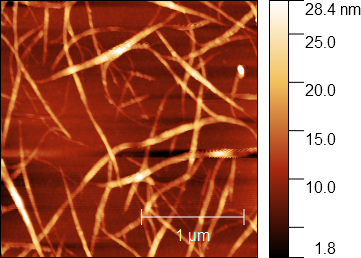
\includegraphics{figures/ch6/Ned_NTQ24_20220125_00235.png}

}

}

\subcaption{\label{fig-bundled-network}}
\end{minipage}%
%
\begin{minipage}[t]{0.05\linewidth}

{\centering 

~

}

\end{minipage}%
%
\begin{minipage}[t]{0.47\linewidth}

{\centering 

\raisebox{-\height}{

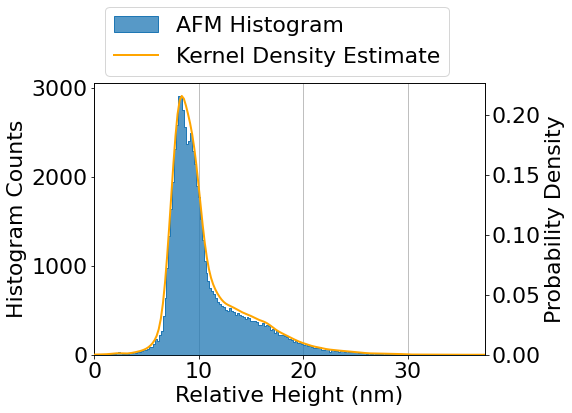
\includegraphics{figures/ch6/Ned_NTQ24_20220125_00235_histogram_initialguess.png}

}

}

\subcaption{\label{fig-bundled-network-histogram}}
\end{minipage}%
\newline
\begin{minipage}[t]{0.47\linewidth}

{\centering 

\raisebox{-\height}{

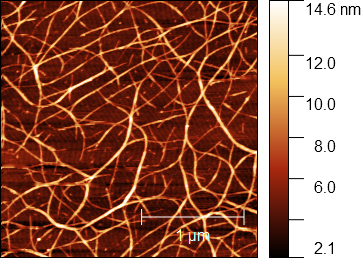
\includegraphics{figures/ch6/Ned_NTQ8C7_w4_pristine_00084_20210428(2).png}

}

}

\subcaption{\label{fig-dropcast-network}}
\end{minipage}%
%
\begin{minipage}[t]{0.05\linewidth}

{\centering 

~

}

\end{minipage}%
%
\begin{minipage}[t]{0.47\linewidth}

{\centering 

\raisebox{-\height}{

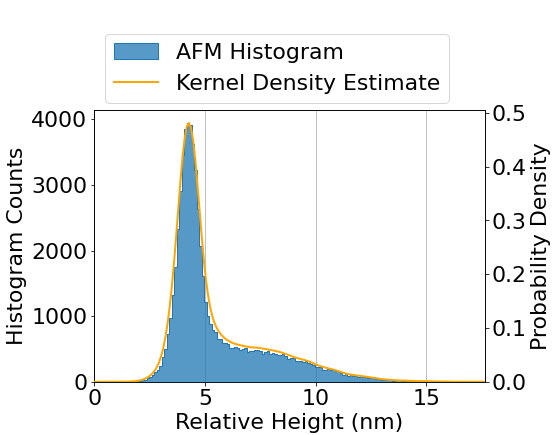
\includegraphics{figures/ch6/Ned_NTQ8C7_w4_pristine_00084_20210428(2)_histogram_initialguess.png}

}

}

\subcaption{\label{fig-dropcast-network-histogram}}
\end{minipage}%
\newline
\begin{minipage}[t]{0.47\linewidth}

{\centering 

\raisebox{-\height}{

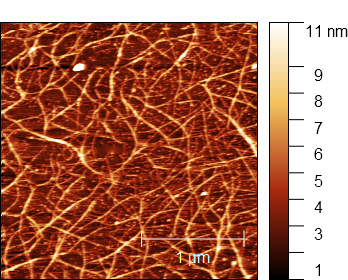
\includegraphics{figures/ch6/Ned_NGQ14D2_W4_pristine_20220713_00567.png}

}

}

\subcaption{\label{fig-steaming-network}}
\end{minipage}%
%
\begin{minipage}[t]{0.05\linewidth}

{\centering 

~

}

\end{minipage}%
%
\begin{minipage}[t]{0.47\linewidth}

{\centering 

\raisebox{-\height}{

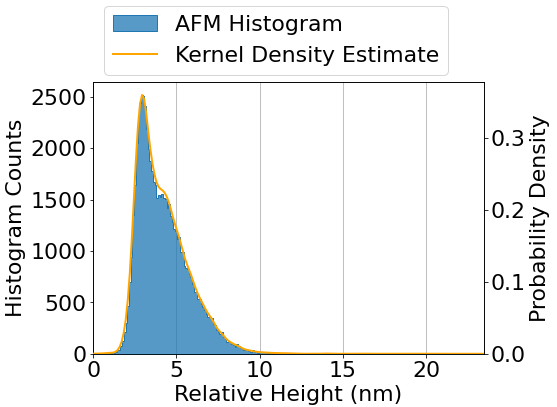
\includegraphics{figures/ch6/Ned_NGQ14D2_W4_pristine_20220713_00567_histogram_initialguess.png}

}

}

\subcaption{\label{fig-steaming-network-histogram}}
\end{minipage}%

\caption{\label{fig-afm-morphology}2.5 \(\mu\)m \(\times\) 2.5 \(\mu\)m
atomic force microscope (AFM) images of carbon nanotube films deposited
using various methods, shown side-by-side with histogram height
distributions and kernel density estimate (KDE) plots corresponding to
each image. The network shown in (a) with height distribution shown in
(b) was deposited in solvent, the network shown in (c) with height
distribution shown in (d) was dropcast in surfactant, and the network
shown in (e) with height distribution shown in (f) was dropcast in
surfactant with steam present.}

\end{figure}

It has previously been demonstrated that the diameter range of deposited
single-walled carbon nanotubes can be modelled via a normal or Gaussian
distribution \autocite{LeMieux2008,Liu2013,Vobornik2023}. However, when
the height profiles from the 2.5 \(\mu\)m \(\times\) 2.5 \(\mu\)m AFM
images are directly extracted and binned, as plotted in black in
Figure~\ref{fig-afm-morphology}, the histograms obtained do not follow a
normal distribution. One reason for this result is the surface roughness
of the silicon dioxide substrate. The carbon nanotubes do not lie
perfectly level on a perfectly level silicon oxide substrate. In
practice, both the SiO\(_2\) substrate and the surface of the carbon
nanotubes both have a degree of roughness. To find the contribution of
surface roughness to the height profile histogram corresponding to each
network deposition method, silicon dioxide substrates were modified
using the same processes as in Figure~\ref{fig-afm-morphology} but
without carbon nanotubes present in the solutions used. 2.5 \(\mu\)m
\(\times\) 2.5 \(\mu\)m AFM images of the modified surfaces are shown in
Figure~\ref{fig-afm-substrate}.

\begin{figure}

\begin{minipage}[t]{0.47\linewidth}

{\centering 

\raisebox{-\height}{

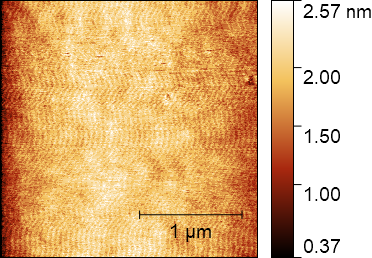
\includegraphics{figures/ch6/Ned_SiO2_00351_20231016.png}

}

}

\subcaption{\label{fig-sio2-only}}
\end{minipage}%
%
\begin{minipage}[t]{0.05\linewidth}

{\centering 

~

}

\end{minipage}%
%
\begin{minipage}[t]{0.47\linewidth}

{\centering 

\raisebox{-\height}{

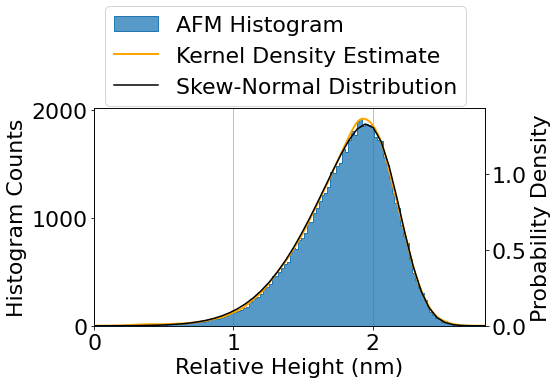
\includegraphics{figures/ch6/Ned_SiO2_00351_20231016_histogram_initialguess.png}

}

}

\subcaption{\label{fig-sio2-histogram}}
\end{minipage}%
\newline
\begin{minipage}[t]{0.47\linewidth}

{\centering 

\raisebox{-\height}{

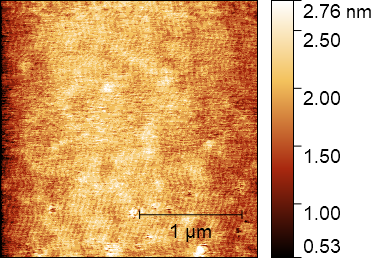
\includegraphics{figures/ch6/Ned_SiO2_s_surfactant_nosteam_00355_20231016.png}

}

}

\subcaption{\label{fig-surfactant-afm}}
\end{minipage}%
%
\begin{minipage}[t]{0.05\linewidth}

{\centering 

~

}

\end{minipage}%
%
\begin{minipage}[t]{0.47\linewidth}

{\centering 

\raisebox{-\height}{

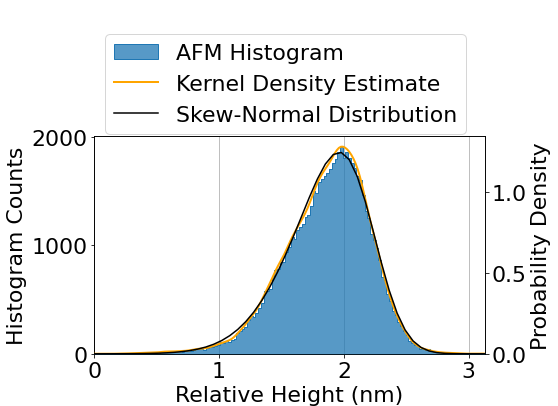
\includegraphics{figures/ch6/Ned_SiO2_s_surfactant_nosteam_00355_20231016_histogram_initialguess.png}

}

}

\subcaption{\label{fig-surfactant-histogram}}
\end{minipage}%
\newline
\begin{minipage}[t]{0.47\linewidth}

{\centering 

\raisebox{-\height}{

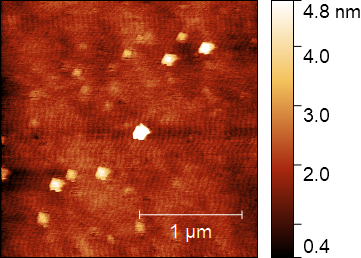
\includegraphics{figures/ch6/Ned_SiO2_s_surfactant_steam_00357_20231016.png}

}

}

\subcaption{\label{fig-steamed-surfactant}}
\end{minipage}%
%
\begin{minipage}[t]{0.05\linewidth}

{\centering 

~

}

\end{minipage}%
%
\begin{minipage}[t]{0.47\linewidth}

{\centering 

\raisebox{-\height}{

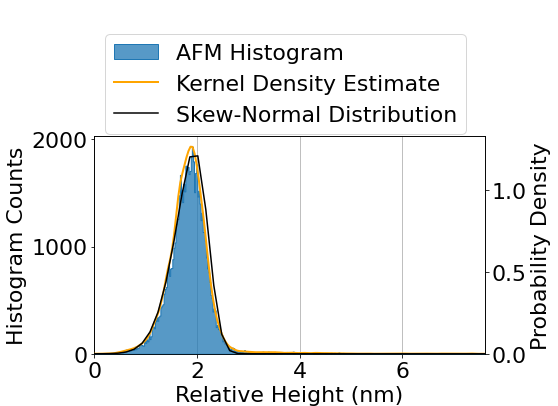
\includegraphics{figures/ch6/Ned_SiO2_s_surfactant_steam_00357_20231016_histogram_initialguess.png}

}

}

\subcaption{\label{fig-steamed-surfactant-histogram}}
\end{minipage}%

\caption{\label{fig-afm-substrate}2.5 \(\mu\)m \(\times\) 2.5 \(\mu\)m
atomic force microscope (AFM) images of silicon dioxide substrates
alongside histogram height distributions and KDE plots corresponding to
each image. The substrate in (a) and (b) was exposed to solvent, the
substrate in (c) and (d) was exposed to surfactant, and the substrate in
(e) and (f) was exposed to surfactant with steam present.}

\end{figure}

In Figure~\ref{fig-afm-substrate}, it appears that each substrate
surface has a roughness that follows a normal distribution with some
degree of skewness. Figure~\ref{fig-sio2-histogram} and
Figure~\ref{fig-surfactant-histogram} are negatively skewed
distributions. The fitted skew-normal distribution in
Figure~\ref{fig-sio2-histogram} has a skew parameter \(\alpha\) (or
shape parameter) of -3.2, a location parameter \(\xi\) of 2.2 nm and a
scale parameter \(\omega\) of 0.5 nm, while in
Figure~\ref{fig-surfactant-histogram} \(\alpha = -2.2\), \(\xi = 2.2\)
nm and \(\omega = 0.5\) nm. \(\xi\) and \(\omega\) correspond to the
mean and standard deviation of the skew-free normal distribution when
\(\alpha\) is set equal to zero \autocite{Azzalini1999}. The close
correspondence between \(\xi\) and \(\omega\) for these distributions
but not \(\alpha\) implies that the skewness is a variable imaging or
processing artifact rather than a physical property of the surface.
Without distortion, the roughness of a clean SiO\(_2\) surface should
follow a normal distribution \autocite{Velicky2015}.

However, Figure~\ref{fig-steamed-surfactant-histogram} has a pronounced
positive skew with a long tail. The tail appears to result from the
contribution of residual surfactant aggregates to surface morphology,
observed in Figure~\ref{fig-steamed-surfactant} and recently discussed
elsewhere in the literature \autocite{Christensen2022,Vobornik2023}.
Attempting to fit a skew-normal distribution to this histogram fails
when all three variables are allowed to vary due to the presence of the
tail. Instead, previous values obtained for \(\xi\) and \(\omega\) can
be used for the fitting process, with only \(\alpha\) allowed to change.
Fixing \(\xi\) and \(\omega\) at 2.2 nm and 0.5 nm respectively gives
the result shown in Figure~\ref{fig-steamed-surfactant-histogram}. The
fitted distribution has an \(\alpha\) of -2.4. The distribution closely
fits the negative tail of the histogram, but deviates slightly from the
positive tail due to the presence of surfactant. Since this deviation is
small, the quality of the fit is still reasonably high, with an
R-squared value of 0.98. Surfactant contamination could have negative
effects on both sensitivity of carbon nanotubes and also could damage
attached biological elements.

\begin{figure}

\begin{minipage}[t]{0.47\linewidth}

{\centering 

\raisebox{-\height}{

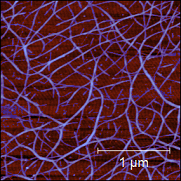
\includegraphics{figures/ch6/Ned_NTQ8C7_w4_pristine_00084_20210428(2)_mask.png}

}

}

\subcaption{\label{fig-mask}}
\end{minipage}%
%
\begin{minipage}[t]{0.05\linewidth}

{\centering 

~

}

\end{minipage}%
%
\begin{minipage}[t]{0.47\linewidth}

{\centering 

\raisebox{-\height}{

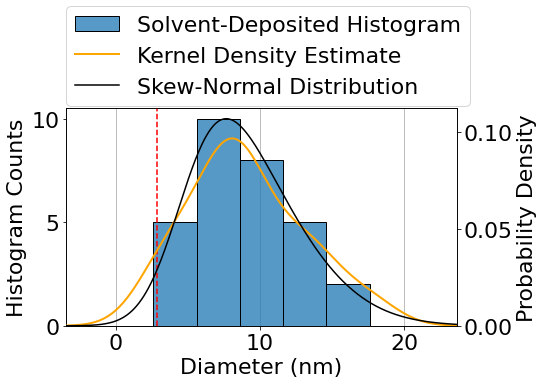
\includegraphics{figures/ch6/NTQ24_20220125_00235_cnt_histogram.png}

}

}

\subcaption{\label{fig-solvent-cnt-histogram}}
\end{minipage}%
\newline
\begin{minipage}[t]{0.47\linewidth}

{\centering 

\raisebox{-\height}{

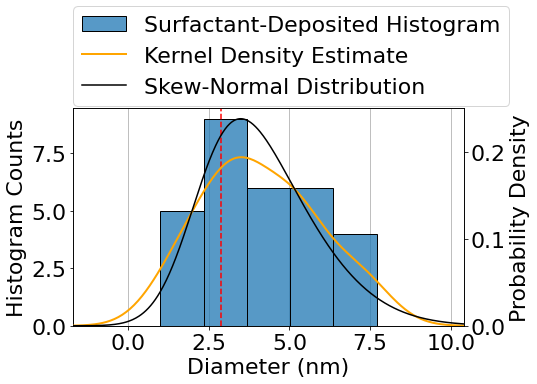
\includegraphics{figures/ch6/NTQ8C7_w4_pristine_cnt_histogram.png}

}

}

\subcaption{\label{fig-surfactant-cnt-histogram}}
\end{minipage}%
%
\begin{minipage}[t]{0.05\linewidth}

{\centering 

~

}

\end{minipage}%
%
\begin{minipage}[t]{0.47\linewidth}

{\centering 

\raisebox{-\height}{

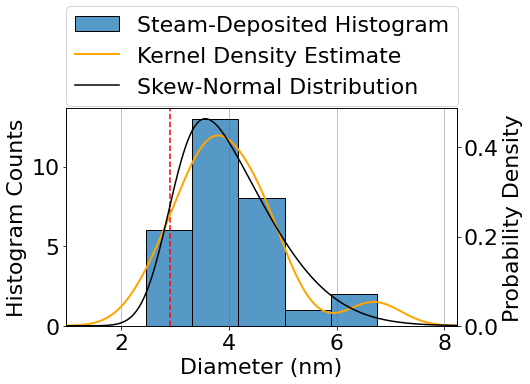
\includegraphics{figures/ch6/NT14D2_W4_pristine_cnt_histogram.png}

}

}

\subcaption{\label{fig-steamed-surfactant-cnt-histogram}}
\end{minipage}%

\caption{\label{fig-cnt-histogram}An masked AFM image is shown in (a),
where the masked carbon nanotube bundles are shaded blue. The mask sets
a height threshold so that masked features are excluded from the height
dataset. Histogram height distributions with corresponding KDE plots
collected via the morphology analysis method outlined by Vobornik
\emph{et al.} \autocite{Vobornik2023} are shown in (b)-(d). The
substrate in (b) was exposed to solvent, the substrate in (c) was
exposed to surfactant, and the substrate in (d) was exposed to
surfactant with steam present.}

\end{figure}

Using the morphology analysis technique outlined by Vobornik \emph{et
al.} \autocite{Vobornik2023}, five successive diameter measurements of
30 carbon nanotube bundles were collected using Gwyddion. Measurements
were not taken at bundle junctions. A height threshold `mask' was
defined in Gwyddion to determine average substrate height, as shown in
Figure~\ref{fig-mask}. This background value was subtracted from our
diameter measurements to determine the actual bundle height. The means
of the solvent-deposited, surfactant-deposited and steam-assisted
surfactant-deposited bundle diameter histograms are \(8.8 \pm 4.0\) nm,
\(4.2 \pm 1.8\) nm and \(3.3 \pm 1.0\) nm respectively. An increased
maximum feature height leads to an increased mean background height, and
by examining the AFM images in Figure~\ref{fig-afm-morphology} it
appears this may be due to deep artifacts on the surface of the
substrate in the vicinity of large features. The average of the five
height-adjusted values for each carbon nanotube bundle was then
calculated, and these 30 averages were sorted into six equal-sized bins.
The binned bundle diameter measurements, alongside estimated probability
density, are shown in Figure~\ref{fig-cnt-histogram}.

From Figure~\ref{fig-cnt-histogram}, it is clear that each histogram
appears to follow a positively skewed normal distribution, different to
the skew-free normal distribution expected from previous works
\autocite{LeMieux2008,Liu2013,Vobornik2023}. The skew is likely another
artifact from imaging the network with the atomic force microscope. The
force of the atomic force microscope tip is known to cause larger
bundles to undergo some degree of compression, and the resulting
systematic underestimation of their height may be responsible for the
distribution skewness \autocite{Vobornik2023}. The fitted skew-normal
distribution in Figure~\ref{fig-solvent-cnt-histogram} has
\(\alpha = 2.7\), \(\xi = 4.3\) nm, \(\omega = 5.9\) nm, the
distribution in Figure~\ref{fig-surfactant-cnt-histogram} has
\(\alpha = 2.4\), \(\xi = 2.2\) nm, \(\omega = 2.6\) nm, and the
distribution in Figure~\ref{fig-steamed-surfactant-cnt-histogram} has
\(\alpha = 3.6\), \(\xi = 2.2\) nm and \(\omega = 1.5\) nm. The
probability density for the carbon nanotube bundle histogram drops to
approximately zero at or before 0 nm, which is physically appropriate.

\begin{verbatim}
Warning: package 'kableExtra' was built under R version 4.3.3
\end{verbatim}

\hypertarget{tbl-circle-packing}{}
\begin{longtable}[]{@{}
  >{\raggedright\arraybackslash}p{(\columnwidth - 16\tabcolsep) * \real{0.1053}}
  >{\raggedright\arraybackslash}p{(\columnwidth - 16\tabcolsep) * \real{0.1228}}
  >{\raggedright\arraybackslash}p{(\columnwidth - 16\tabcolsep) * \real{0.0965}}
  >{\raggedright\arraybackslash}p{(\columnwidth - 16\tabcolsep) * \real{0.0965}}
  >{\raggedright\arraybackslash}p{(\columnwidth - 16\tabcolsep) * \real{0.1228}}
  >{\raggedright\arraybackslash}p{(\columnwidth - 16\tabcolsep) * \real{0.1228}}
  >{\raggedright\arraybackslash}p{(\columnwidth - 16\tabcolsep) * \real{0.1228}}
  >{\raggedright\arraybackslash}p{(\columnwidth - 16\tabcolsep) * \real{0.1228}}
  >{\raggedright\arraybackslash}p{(\columnwidth - 16\tabcolsep) * \real{0.0877}}@{}}
\caption{\label{tbl-circle-packing}The first eight optimised ratios of
2D packed circle diameter to encompassing circle diameter, given to 3
s.f. (encompassing circle diameter = \(d\), number of packed circles =
\(n\), approximate packed circle diameter = \(d_n\)).\\
}\tabularnewline
\toprule\noalign{}
\endfirsthead
\endhead
\bottomrule\noalign{}
\endlastfoot
\(n\) & \text{2} & \text{3} & \text{4} & \text{5} & \text{6} & \text{7}
& \text{8} & \text{9} \\
\(d\)/\(d_n\) & \text{2.00} & 2.15 & 2.41 & \text{2.70} & \text{3.00} &
\text{3.00} & \text{3.30} & 3.61 \\
\end{longtable}

Previously, analysis of the morphology of carbon nanotube networks has
been simplified by assuming the component nanotubes are cylinders,
follow 2D packing and are of equal diameter \autocite{Murugathas2018}.
Table~\ref{tbl-circle-packing} shows the relationship between the
diameter of a bundle of 2D packed cylinders and the constituent
diameters of up to nine cylinders within that bundle. From looking up
the relevant \(d\)/\(d_n\) packing ratios, and assuming an average
carbon nanotube diameter of 1.45 nm, it is possible to use to find the
approximate number of nanotubes \emph{n} likely to be present in the
mean bundle size corresponding to each deposition type
\autocite{Graham1998,Specht2023}. These estimates are shown in
Table~\ref{tbl-histogram-parameters}. Also shown in
Table~\ref{tbl-histogram-parameters} is an estimate of the ratio of
single- to multi-tube bundles for each deposition. This estimate was
obtained by taking the integral of each distribution with a lower bound
of 2.9 nm, the minimum multi-tube bundle size for 1.45 nm diameter
nanotubes. As the area under the curve represents the probability a
bundle will have a particular diameter, this integral should give a good
estimate of the relative proportion of multi-tube bundles.
Table~\ref{tbl-histogram-parameters} should be interpreted as
lower-limit estimates of the size and relative proportion of bundles,
recalling that the distribution skewness indicates underestimation of
the true bundle height.

\hypertarget{tbl-histogram-parameters}{}
\begin{longtable}[t]{>{\raggedright\arraybackslash}p{4cm}>{\centering\arraybackslash}p{3cm}>{\centering\arraybackslash}p{3cm}>{\centering\arraybackslash}p{3cm}}
\caption{\label{tbl-histogram-parameters}The mean of histogram distributions for carbon nanotube films deposited
using various methods, alongside estimates for the number of nanotubes
present per mean bundle and the estimated proportion of multi-tubed
bundles present across the network. }\tabularnewline

\toprule
 & Mean Bundle Diameter (nm) & Tubes per Average Bundle & \% Multi-Tube Bundles\\
\midrule
Solvent deposited & 8.8 ± 4.0 & 28 & > 96\%\\
Surfactant deposited & 4.2 ± 1.8 & 5 & > 75\%\\
Surfactant deposited with steam & 3.3 ± 1.0 & 3 & > 65\%\\
\bottomrule
\end{longtable}

Both the carbon nanotube bundle diameter mean and standard deviation are
small for surfactant-deposited films when compared to the mean and
standard deviation of solvent-deposited films. However, despite the
presence of surfactant, it is apparent both from
Figure~\ref{fig-afm-morphology} and Table~\ref{tbl-histogram-parameters}
that not all surfactant-dispersed carbon nanotubes are deposited
individually. Bundling may occur during the process of deposition onto
the substrate, which could disrupt the repulsive forces from the
surfactant coating and allow attractive forces to temporarily dominate.
It is possible that the bundling of surfactant-dispersed carbon
nanotubes is a consequence of dynamics introduced by the coffee-ring
effect \autocite{Deegan1997,VanGaalen2021}. The coffee-ring effect
refers to a build-up of dispersed solid forming around the edges of a
dispersion evaporating on a surface. This process occurs due to the
dispersion edges being fixed by surface forces, leading to capillary
flow outwards to replace liquid evaporating at the edges, bringing solid
material along with it. The presence of vapour is known to disrupt this
capillary effect \autocite{Bishop2020}, which may explain why mean
bundle diameter is lower for the films deposited in surfactant with
steam present relative to films deposited in surfactant without steam.

The discussion in this section gives us a new understanding of the
histograms shown in Figure~\ref{fig-afm-morphology}. It is now apparent
that these histograms are linear combinations of skewed normal
distributions. These distributions include a negatively-skewed
distribution corresponding to the substrate surface and a
positively-skewed distribution corresponding to the carbon nanotube
bundles. X and Y junctions between overlapping nanotubes may also form a
similarly skewed normal distribution as part of the full histogram
\autocite{Murugathas2018}. The complete linear combination could be
modelled mathematically in order to rapidly extract key parameters from
atomic force microscope images \autocite{Marchenko2010}, but
implementing this approach is outside of the scope of this thesis.
Another outcome of this discussion is awareness that carbon nanotube
bundling within a network is lowered by the presence of surfactant
during deposition. Introducing steam when depositing with surfactant
lowers bundling even further, but also leads to residual surfactant
pooling and attaching to the substrate surface. These results may both
be explained by the presence of steam enabling surfactant to follow
carbon nanotubes to the substrate surface, which keeps them from
bundling during the attachment process. The unwanted persistence of
surfactant means that higher temperature vacuum annealing may be
required for robust biosensors \autocite{Kane2014}.

\hypertarget{sec-pristine-raman}{%
\subsection{Raman Spectroscopy}\label{sec-pristine-raman}}

\begin{figure}

\begin{minipage}[t]{0.47\linewidth}

{\centering 

\raisebox{-\height}{

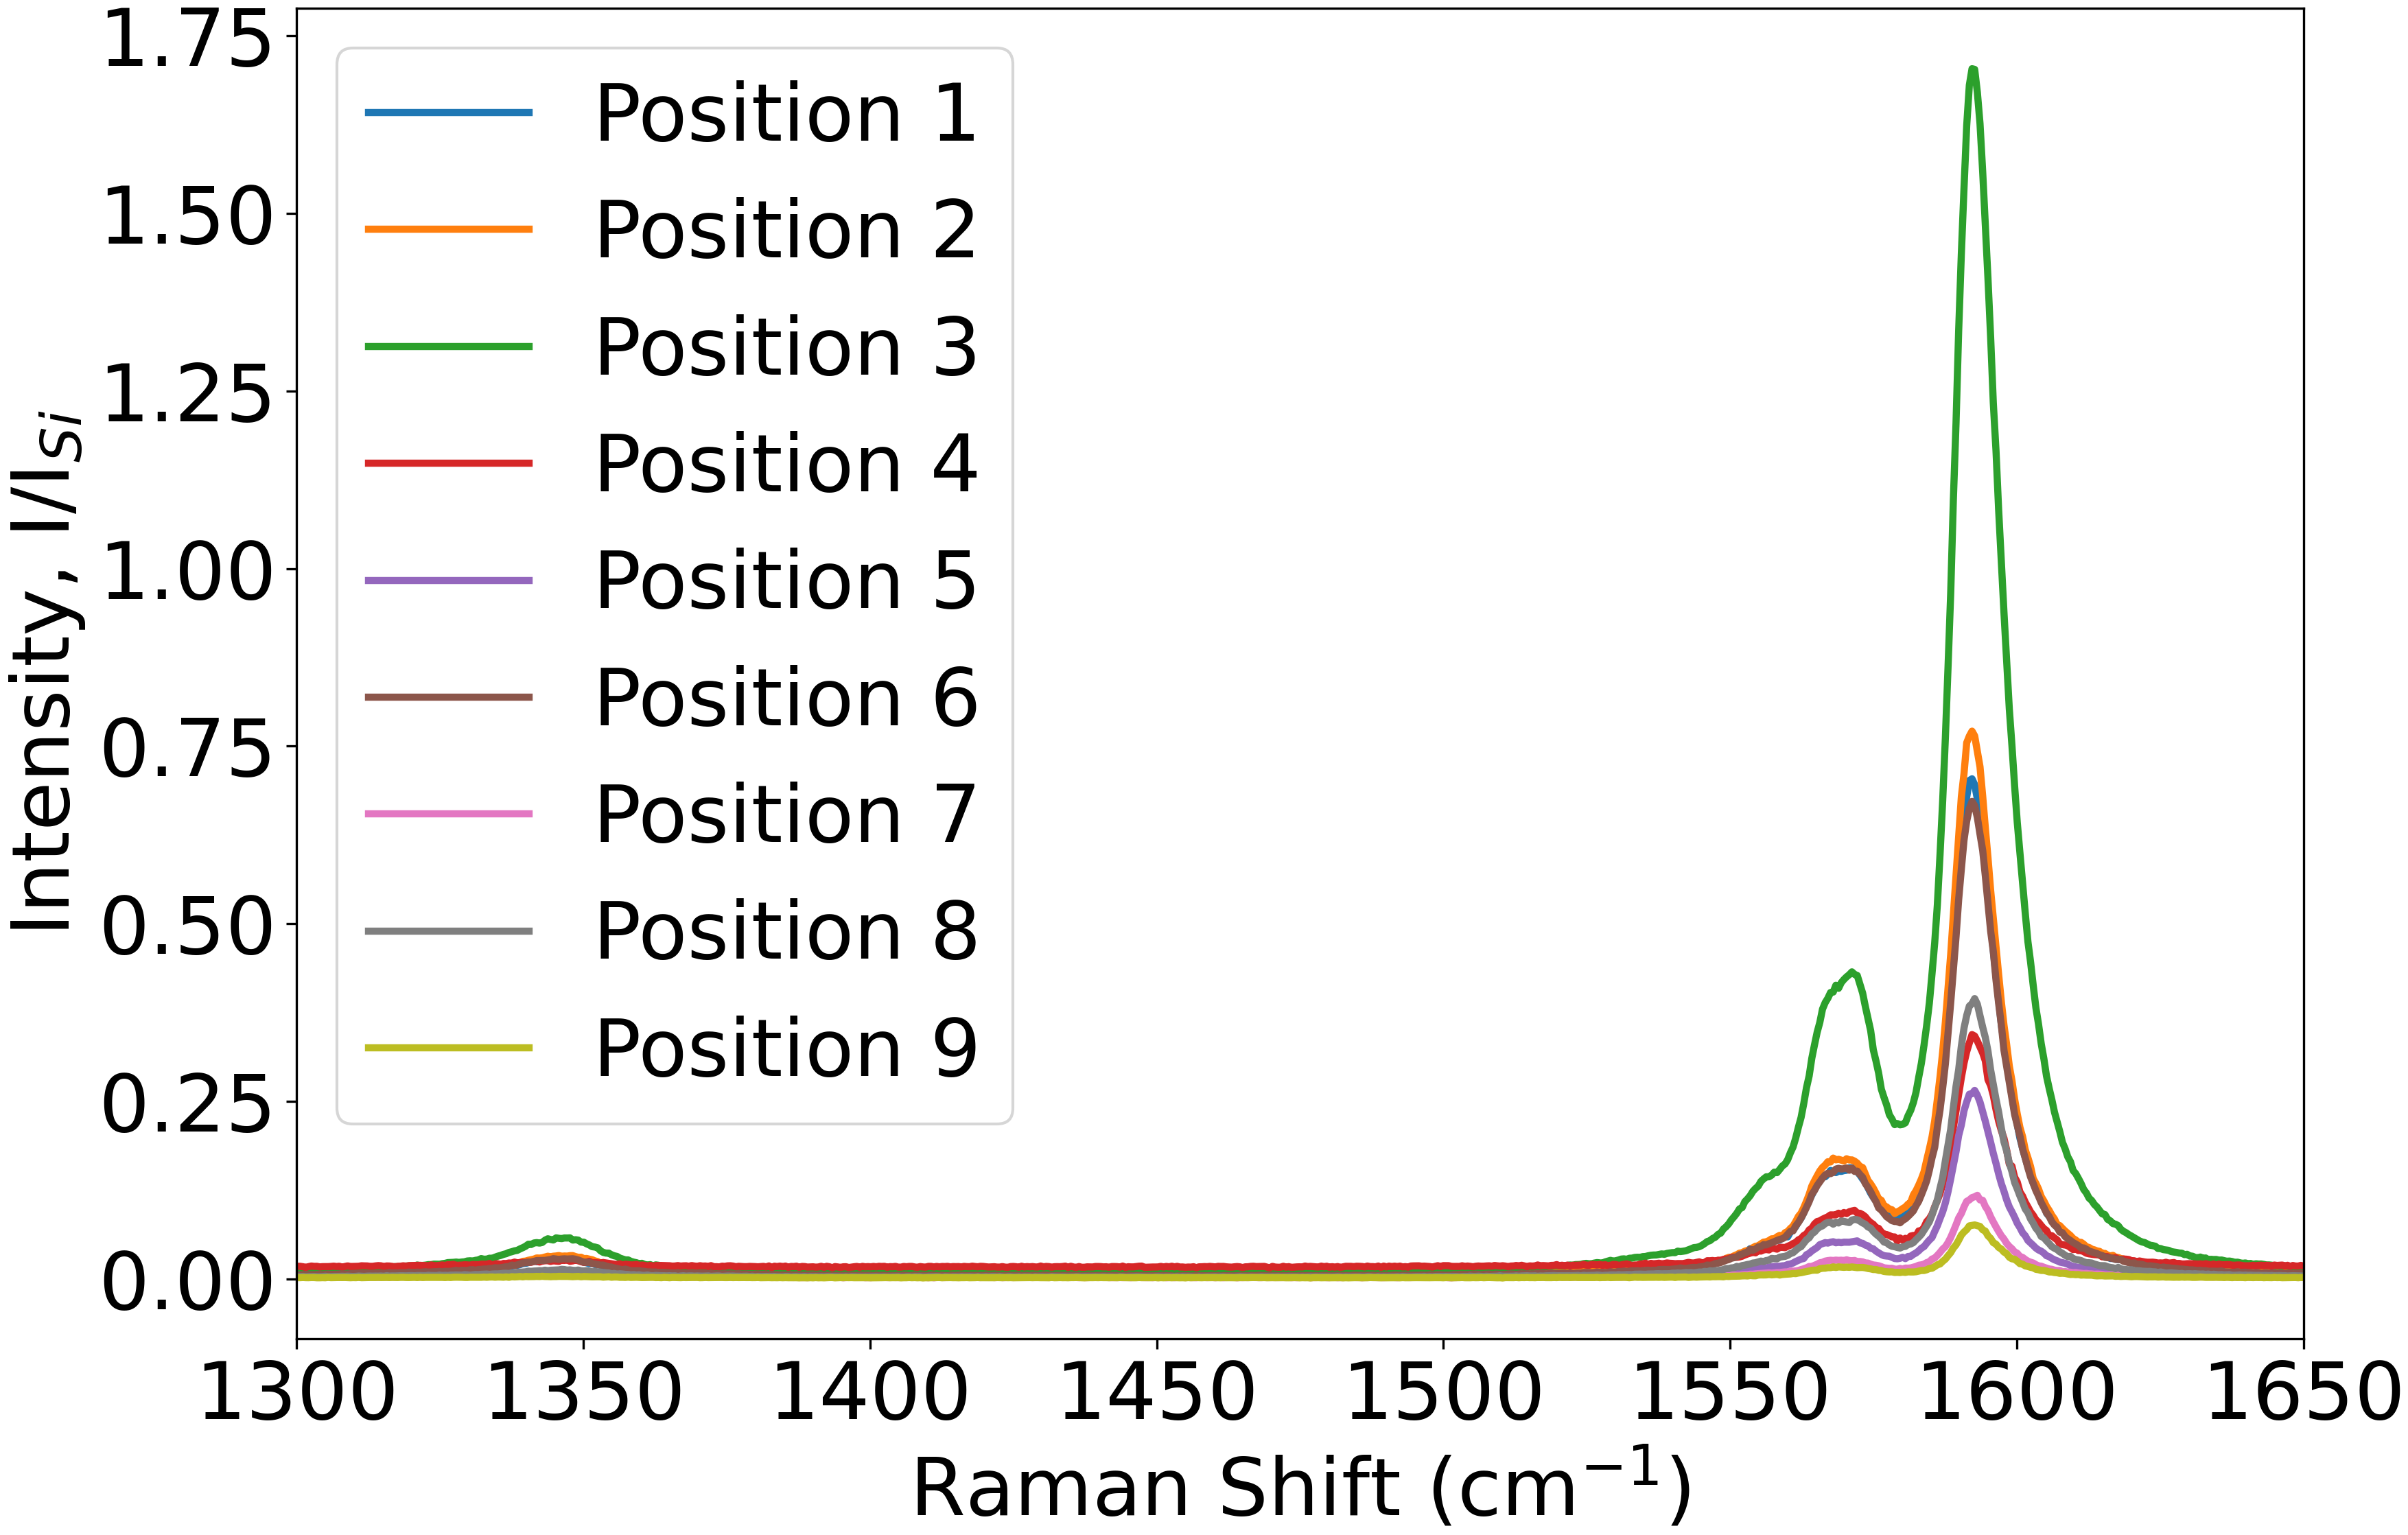
\includegraphics{figures/ch6/bundled_raman.png}

}

}

\subcaption{\label{fig-solvent-deposited}}
\end{minipage}%
%
\begin{minipage}[t]{0.05\linewidth}

{\centering 

~

}

\end{minipage}%
%
\begin{minipage}[t]{0.47\linewidth}

{\centering 

\raisebox{-\height}{

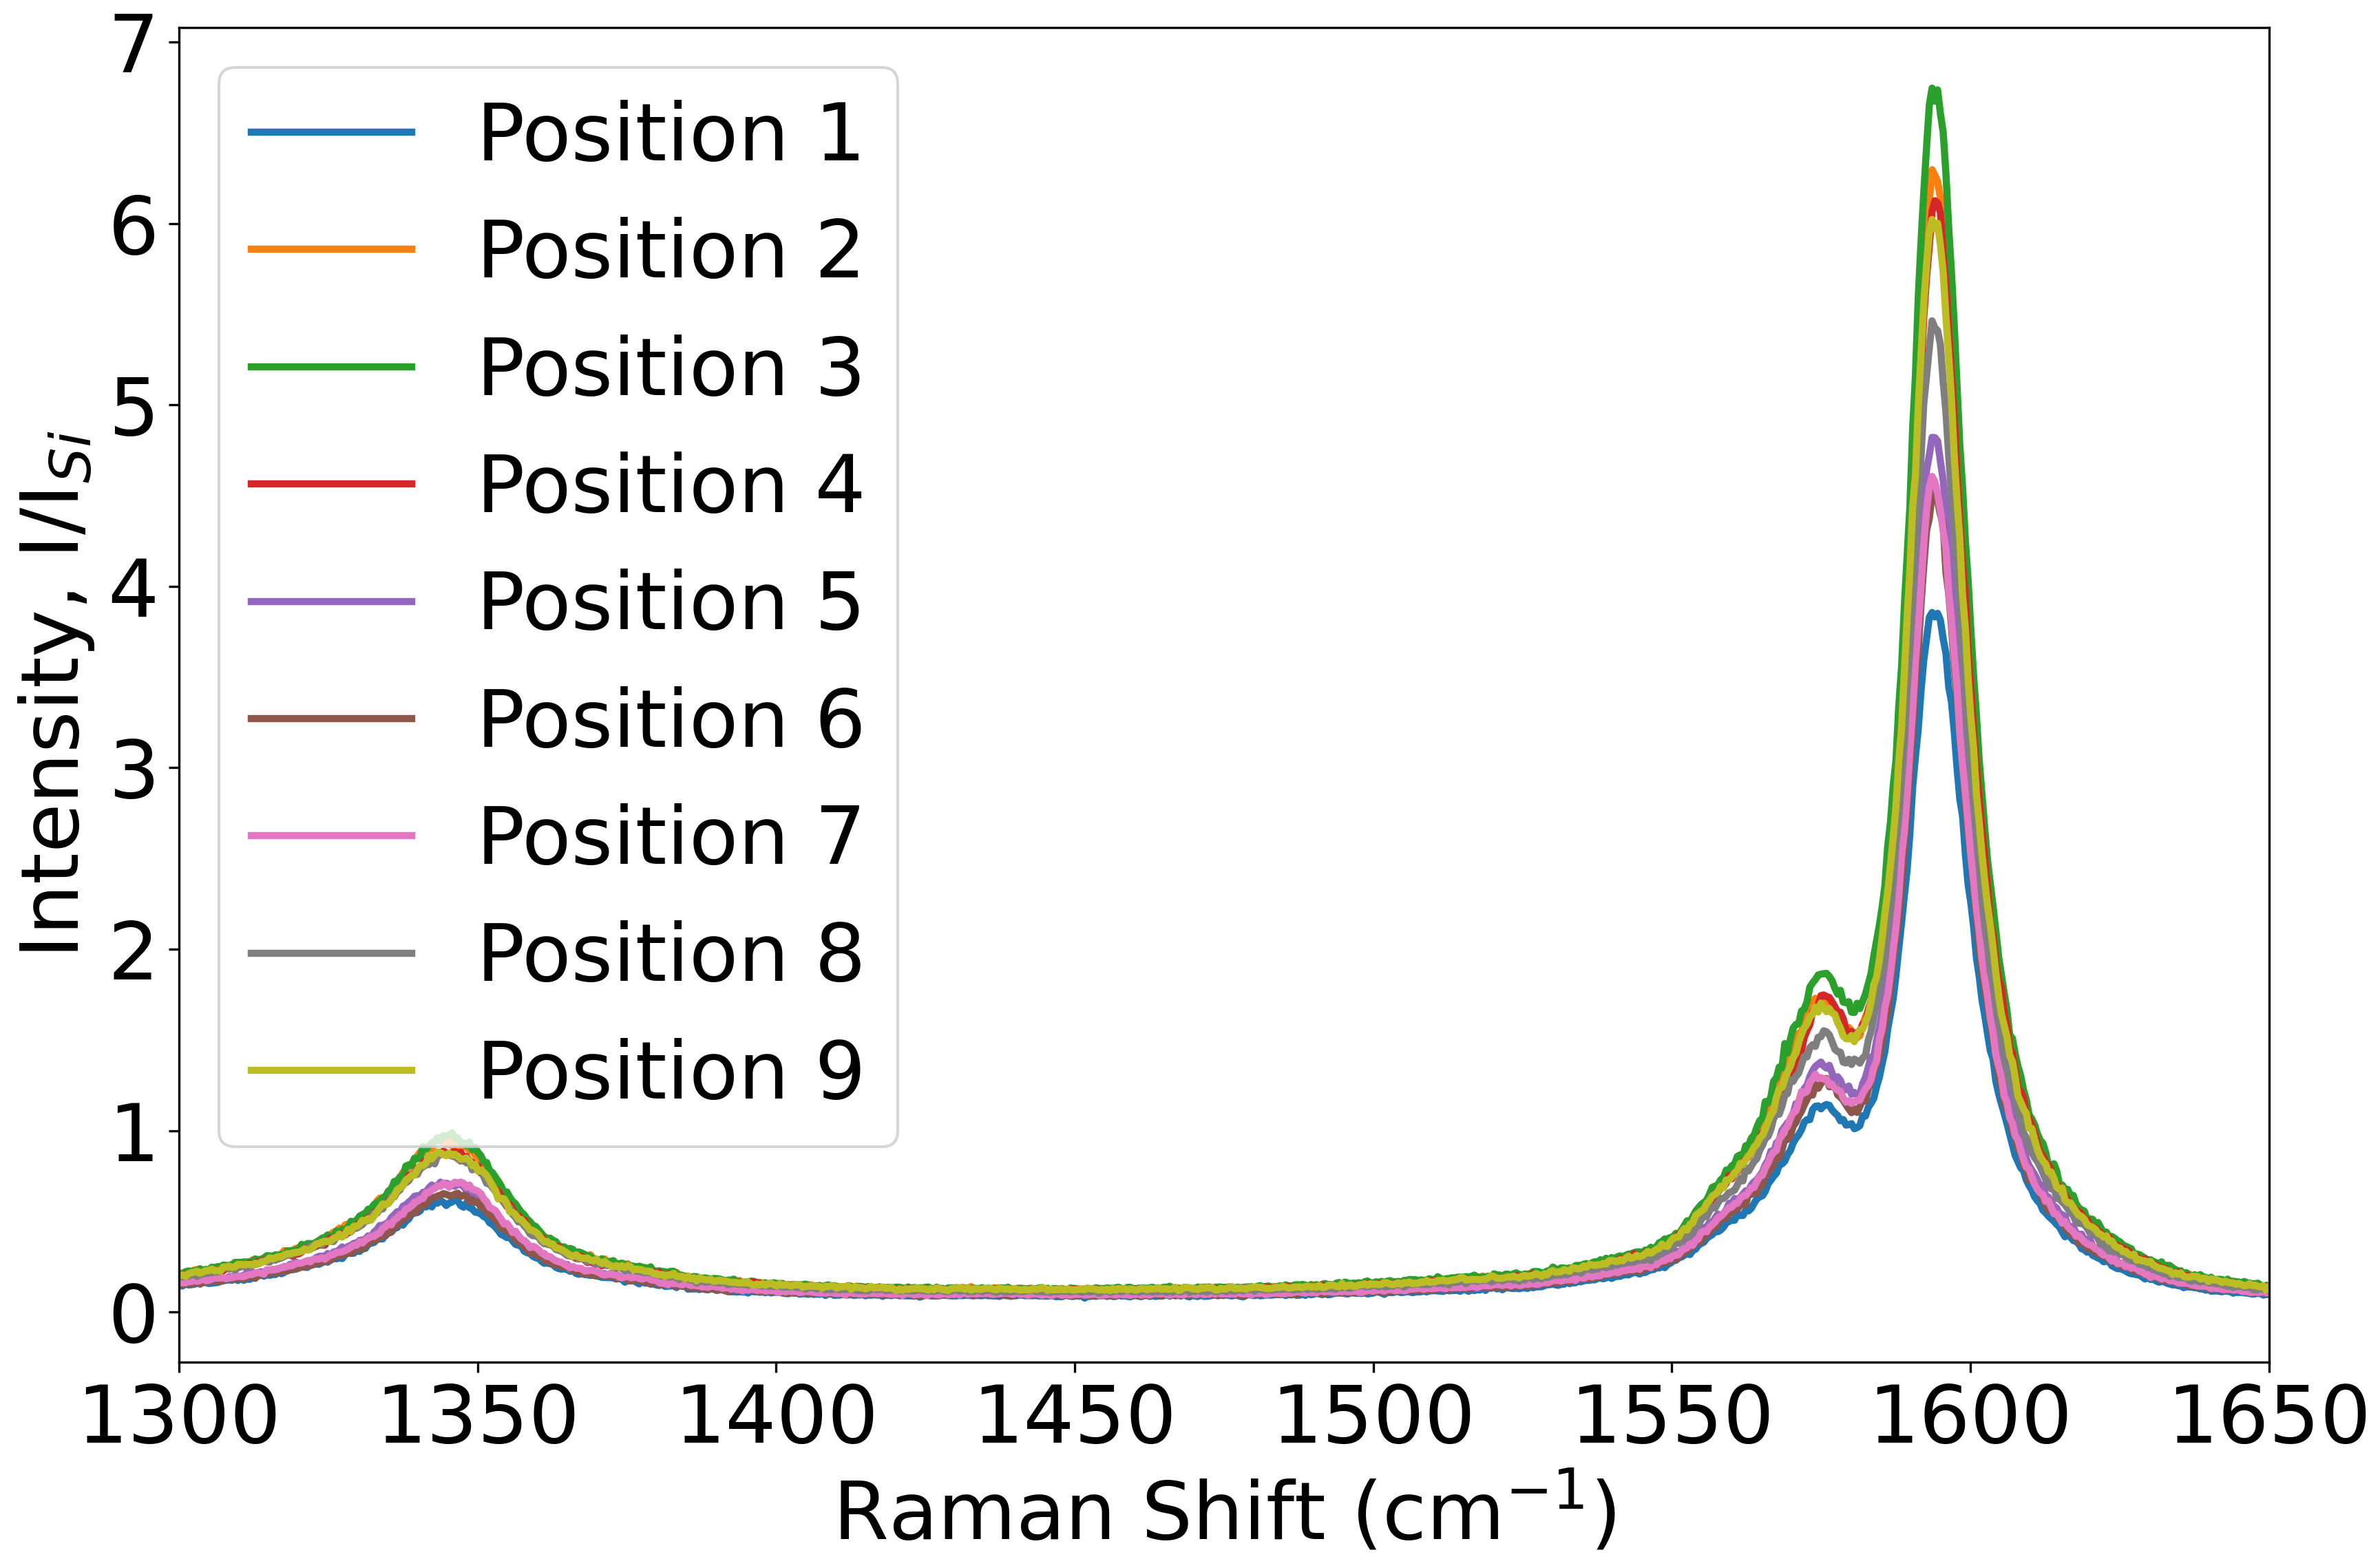
\includegraphics{figures/ch6/singletube_raman.png}

}

}

\subcaption{\label{fig-surfactant-deposited}}
\end{minipage}%
\newline
\begin{minipage}[t]{0.33\linewidth}

{\centering 

~

}

\end{minipage}%
%
\begin{minipage}[t]{0.35\linewidth}

{\centering 

\raisebox{-\height}{

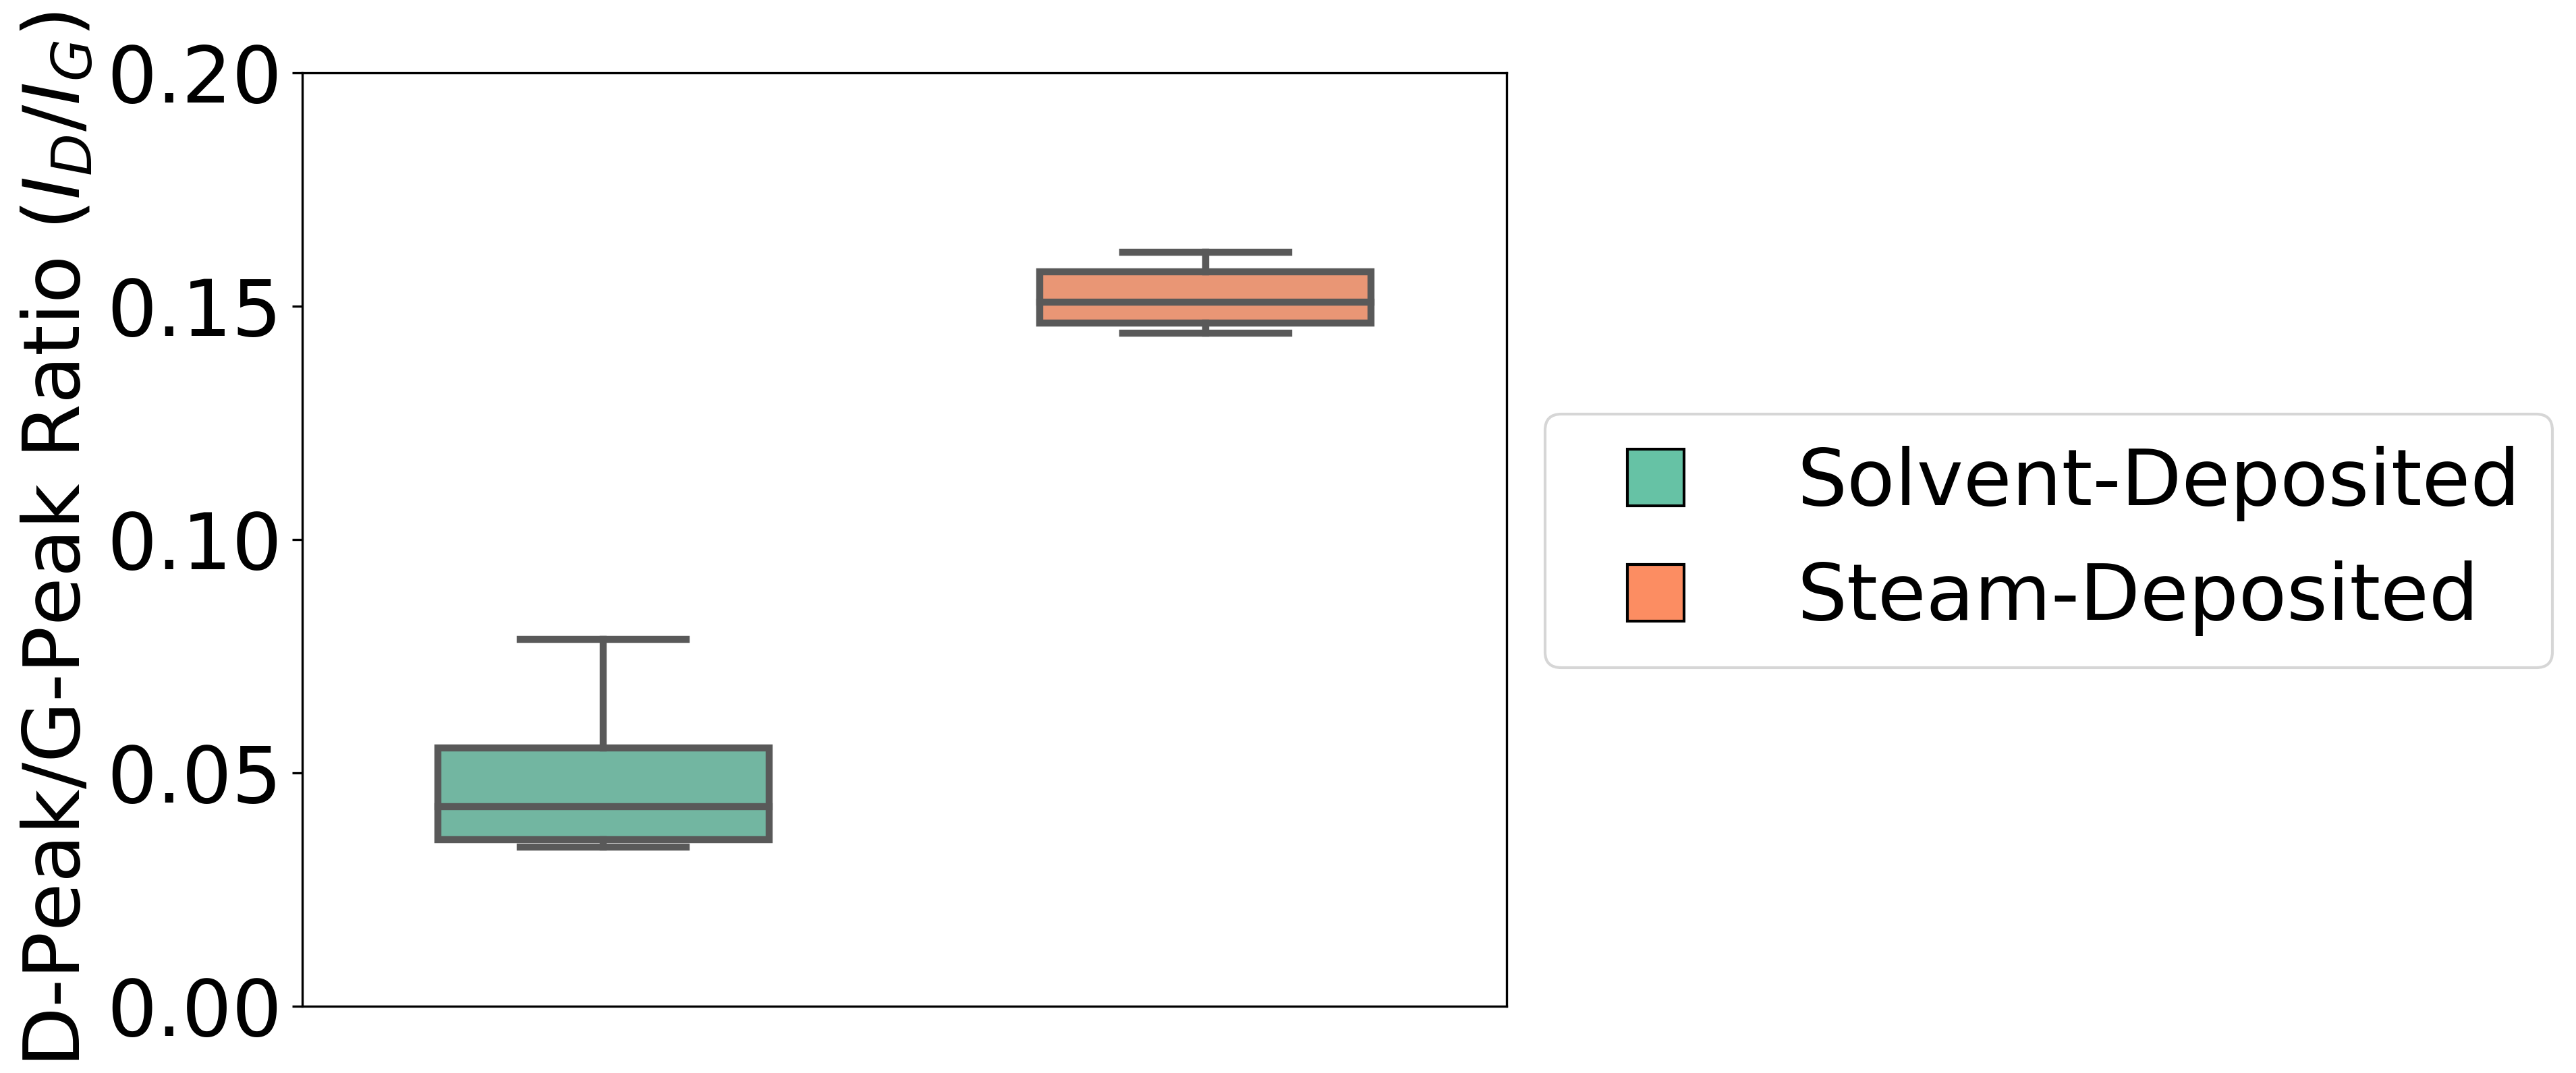
\includegraphics{figures/ch6/comparison-raman.png}

}

}

\subcaption{\label{fig-dg-peak-comparison}}
\end{minipage}%
%
\begin{minipage}[t]{0.33\linewidth}

{\centering 

~

}

\end{minipage}%

\caption{\label{fig-pristine-raman}A series of nine Raman spectra at
different locations across a 40 \(\mu\)m \(\times\) 100 \(\mu\)m carbon
nanotube film region, where (a) shows spectra from a film deposited
using solvent while (b) shows spectra from a film deposited with
surfactant in the presence of steam. (c) shows the spread of the
D-peak/G\(^+\)-peak spectral ratios corresponding to each film.}

\end{figure}

Raman spectroscopy was also used to analyse and compare the deposited
carbon nanotube networks. Raman spectra were collected from a
solvent-deposited carbon nanotube film and a steam-assisted
surfactant-deposited film, both on silicon dioxide, in the manner
described in \textbf{?@sec-raman-characterisation}. These spectra were
then processed using the Python script mentioned in
Section~\ref{sec-raman-analysis}. For each location, spectra over two
wavenumber ranges were collected. A peak corresponding to the silicon
dioxide substrate, found in the range between 100 cm\(^{-1}\) and 650
cm\(^{-1}\), was used as a reference peak for the normalisation of
intensity across the wavenumber range between 1300 cm\(^{-1}\) and 1650
cm\(^{-1}\). These normalised spectra are shown in
Figure~\ref{fig-pristine-raman}. In all spectra, a D-band comprising a
single D-peak is observed at \(\sim\) 1320 cm\(^{-1}\), and a G-band
comprising two G-peaks, G\(^-\) and G\(^+\), is observed between
\(\sim\) 1525 cm\(^{-1}\) and \(\sim\) 1650 cm\(^{-1}\). These features
are characteristic of networks of semiconducting carbon nanotubes
\autocite{Dresselhaus2005,King2014}.

Closer inspection of the D peak and G peaks can give us important
information about network composition. G\(^-\) is a minor peak found at
\(\sim\) 1570 cm\(^{-1}\), while G\(^+\) is a larger feature at \(\sim\)
1590 cm\(^{-1}\). The G\(^+\) feature describes the in-plane vibration
of carbon bonds along the length of the carbon nanotubes, while the
G\(^-\) feature describes the in-plane vibration of bonds about the
nanotube circumference \autocite{King2014,Swiniarski2021}. The splitting
between the wavenumber location of the G\(^-\) and G\(^+\) local maxima
is lower in Figure~\ref{fig-surfactant-deposited} than in
Figure~\ref{fig-solvent-deposited}, indicating more metallic nanotubes
are present in the surfactant-deposited network
\autocite{Swiniarski2021}. The D-peak gives an indication of the defects
present in the carbon nanotube atomic structure
\autocite{King2014,Swiniarski2021}. The size of the normalised D-peak
appears much lower in Figure~\ref{fig-solvent-deposited} than in
Figure~\ref{fig-surfactant-deposited}, indicating the solvent deposition
process introduces less defects to the carbon nanotubes than
surfactant-mediated deposition.

It is also possible to compare the relative magnitude of the D-peak and
G\(^+\)-peak intensity to quantify carbon nanotube structural disorder,
which disrupts in-plane lattice vibration
\autocite{Dresselhaus2005,King2014}. Figure~\ref{fig-dg-peak-comparison}
gives a summary of the ratios between the D-peak and G\(^+\)-peak across
all nine positions for the solvent-deposited and surfactant-deposited
film. It is immediately observed that I\(_{D}\)/I\(_{G}\) is
significantly larger for the steam-assisted, surfactant-deposited films
than for the solvent-deposited films. This is a further indication of
the presence of defects across the steam-deposited network. These
defects are likely introduced through the introduction of charge
impurites by surfactant aggregates present around the carbon nanotubes
\autocite{Christensen2022}. However, at the same time, the range of
values for the I\(_{D}\)/I\(_{G}\) ratio is lower for the
steam-deposited network. This spatially homogeneous vibrational
behaviour implies the steam-deposited network is more evenly distributed
than the solvent-deposited network, which matches the discussion in
Section~\ref{sec-pristine-morphology}.

\hypertarget{sec-pristine-electrical-characterisation}{%
\section{Electrical Characteristics of Pristine
Devices}\label{sec-pristine-electrical-characterisation}}

\hypertarget{sec-python-analysis}{%
\subsection{Python Analysis}\label{sec-python-analysis}}

Analysis of electrical measurements was performed using the three
modules described in Section~\ref{sec-field-effect-transistor-analysis}.
The first of the three modules is for processing sensing datasets. This
module cleans, analyses and filters sensing data and produces a variety
of plots. These plots include normalised plots (type of normalisation
can be set in the code config file), plots with fitted curves, plots
with the linear baseline drift removed, plots of signal with analyte
addition, ``despiked'' plots and ``filtered'' plots. The analysis used
to produce these plots is described further below. It is possible to add
annotations to any of these plots using the config file, and it is
possible to produce a plot with a combination of these modifications.
The module can also fit exponential and linear trendlines to regions of
the sensing data, and find the signal change per analyte addition; the
module then returns spreadsheets containing the results of these
analyses, including the standard deviation for all calculated
parameters.

The scipy.optimize.curve\_fit function is used in the first module to
fit linear and exponential curves to regions of interest of the sensing
data. For a linear fit \(c_1t + c_2\), initial parameters are simply set
as \(c_1=1\) and \(c_2=0\). For an exponential fit
\(I_0\exp{(-t/\tau)} + I_C\), rough approximations are used for the
initial parameters: \(I_C\) is set as the final current measurement of
the region of interest, \(I_0\) is set as the initial current
measurement minus \(I_C\), and \(\tau\) is set as the time where current
has dropped to \(e^{-1}I_0 + I_C\).

``Despiked'' plots have had spurious datapoints removed through the use
of an interquartile range rolling filter. The window size of the rolling
filter used was 40 datapoints, and datapoints in each window with a
z-score above \(\pm 3\) were removed from the plotted/processed data.
``Filtered'' plots had noise reduced using a moving median filter. The
moving median filter is more effective at removing noise than a simple
moving average, and has advantages over other filters (such as the
Savitzky-Golay filter) when removing noise from data with sharp edges,
as is the case for sensing data. Median filtering can also be used for
baseline drift compensation, though this approach was not used in this
thesis \autocite{Stone2011}. The moving median filter used had a window
of 40 datapoints.

Plots of signal with analyte addition were constructed from current data
after first removing baseline drift and applying a moving median filter.
A simple difference calculation between the mean of the filtered current
before an addition and the mean of the filtered current after the
addition was performed at each addition. These differences were then
normalised relative to the initial current. The signal with analyte
addition give reasonably consistent results regardless of whether
baseline drift was removed from the data, as shown in
Figure~\ref{fig-spaa-plot-comparison}. We can therefore be confident
that robust signal with analyte addition plots are robust even in the
presence of significant drift.

\begin{figure}

\begin{minipage}[t]{0.50\linewidth}

{\centering 

\raisebox{-\height}{

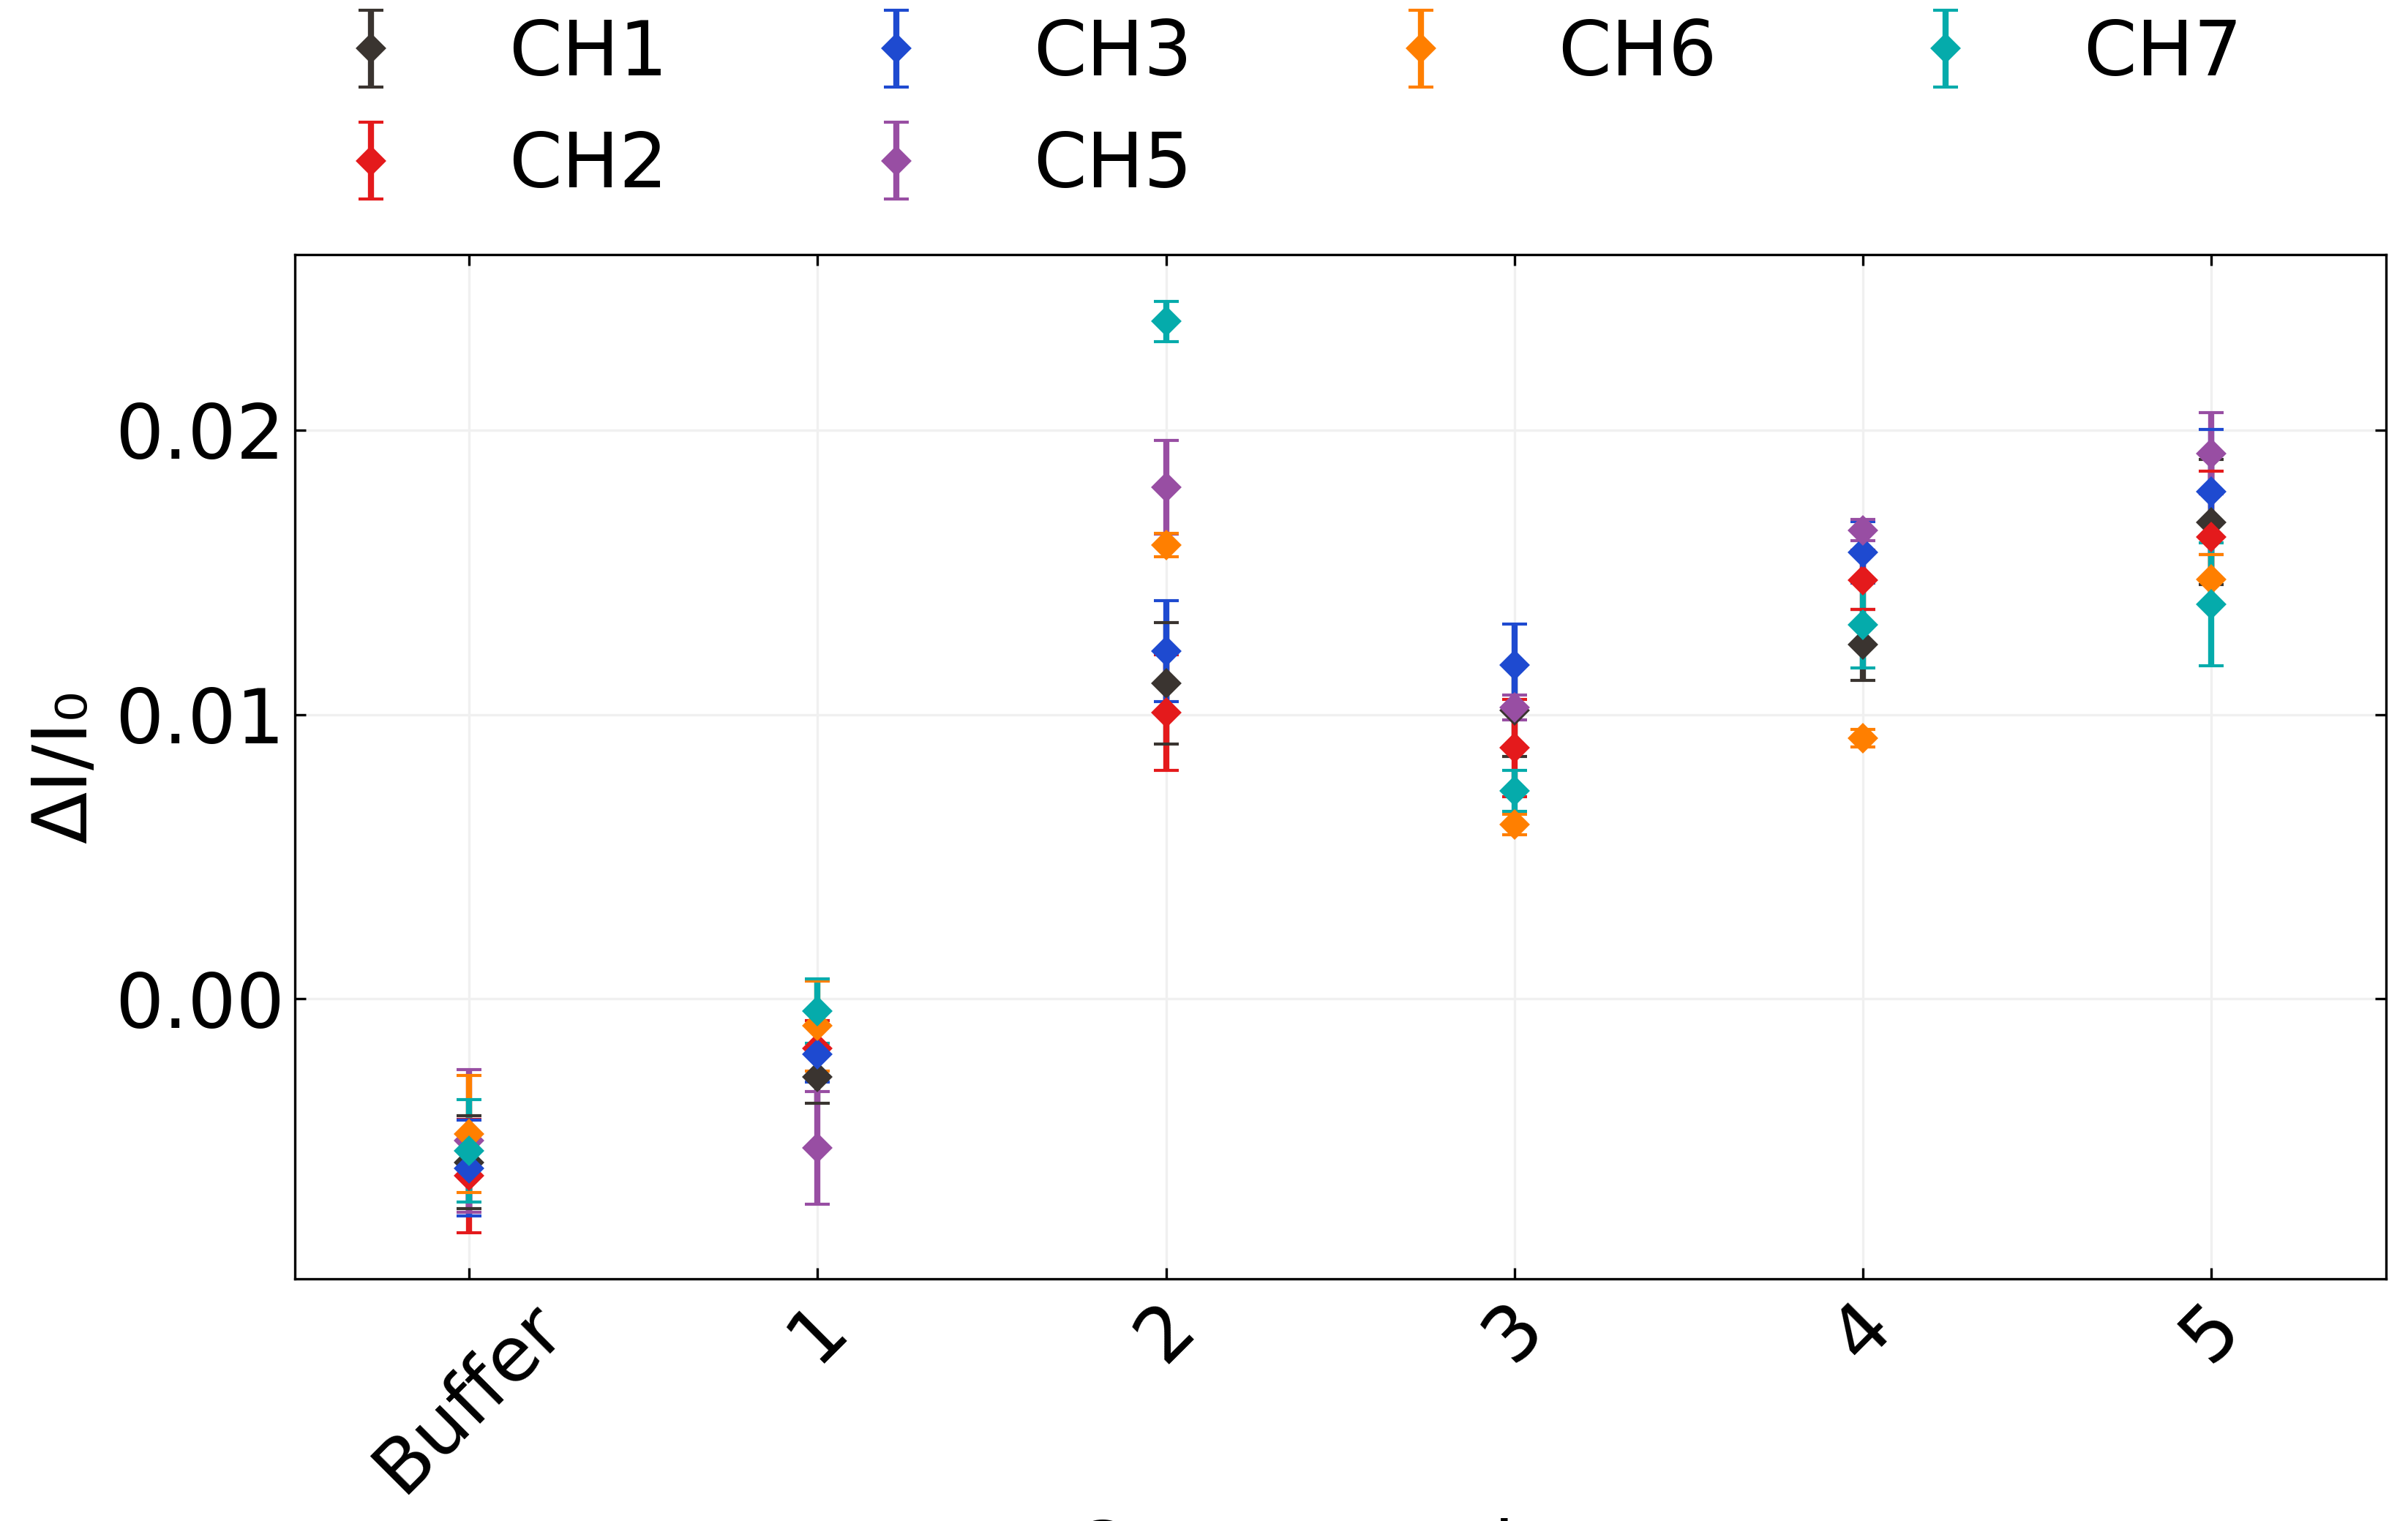
\includegraphics{figures/ch6/NTQ31C1_mean_simple_difference_before_and_after_step_filtered_concentrations.png}

}

}

\subcaption{\label{fig-spaa-no-detrend}}
\end{minipage}%
%
\begin{minipage}[t]{0.50\linewidth}

{\centering 

\raisebox{-\height}{

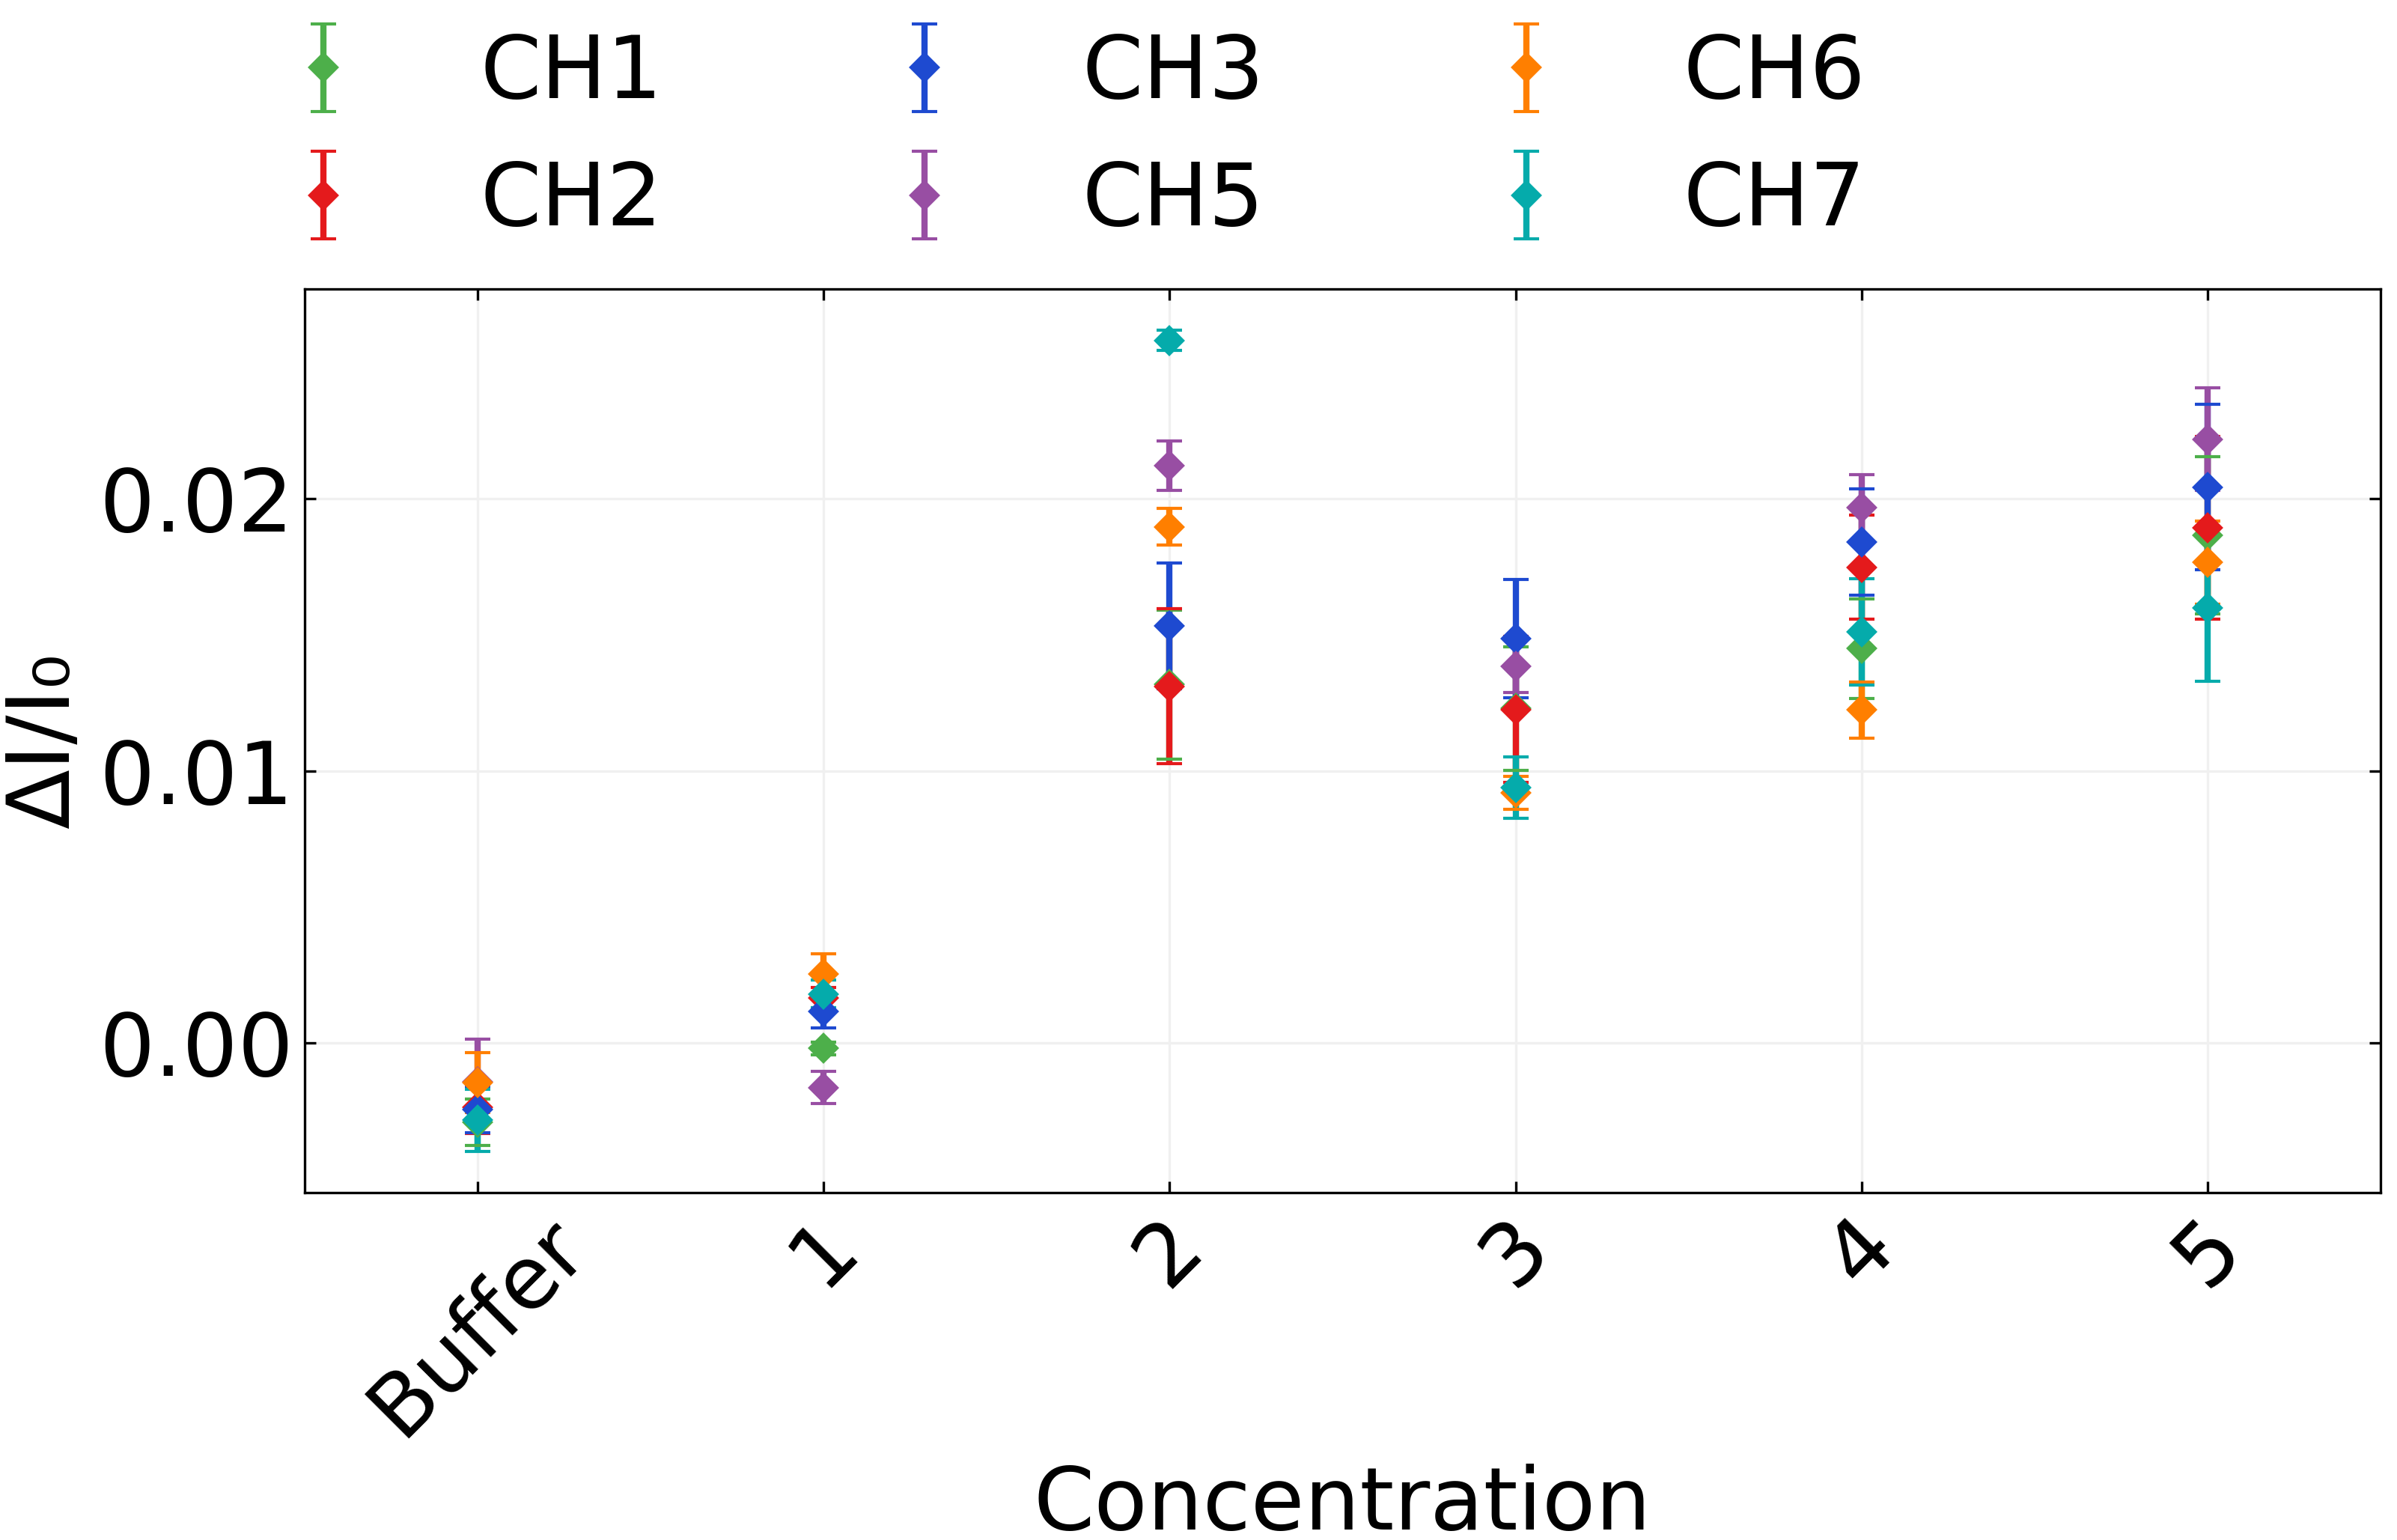
\includegraphics{figures/ch6/NTQ31C1_mean_simple_difference_before_and_after_step_filtered_concentrations_detrend.png}

}

}

\subcaption{\label{fig-spaa-detrend}}
\end{minipage}%

\caption{\label{fig-spaa-plot-comparison}A comparison of signal with
analyte addition plots taken from the same salt concentration sensing
dataset (the same dataset as used in
Figure~\ref{fig-salt-conc-sensing}). In (a), a simple difference
calculation performed on filtered data was used, while in (b) the same
calculation was performed on filtered data with the baseline drift
removed, the method used in the body of the thesis.}

\end{figure}

The second module creates combined and individual plots of transfer data
collected from eight channels on a single device. In combined plots,
channels which are non-working, due to being shorted or non-conducting,
are removed via setting a maximum and minimum possible on-current in the
config file. Various parameters from the transfer characteristics are
saved as a spreadsheet along with standard error. These parameters
include on current, off current, subthreshold slope and threshold
voltage for the carbon nanotube devices, and on current, off current and
major Dirac point voltage for graphene devices. The device type being
analysed can be set in the config file.

The third module allows for comparison of transfer measurements taken of
the same channel before and after some modification. It also calculates
the shift in either threshold voltage or major Dirac voltage of the
device.

\hypertarget{carbon-nanotube-network-devices}{%
\subsection{Carbon Nanotube Network
Devices}\label{carbon-nanotube-network-devices}}

\begin{figure}

\begin{minipage}[t]{0.49\linewidth}

{\centering 

\raisebox{-\height}{

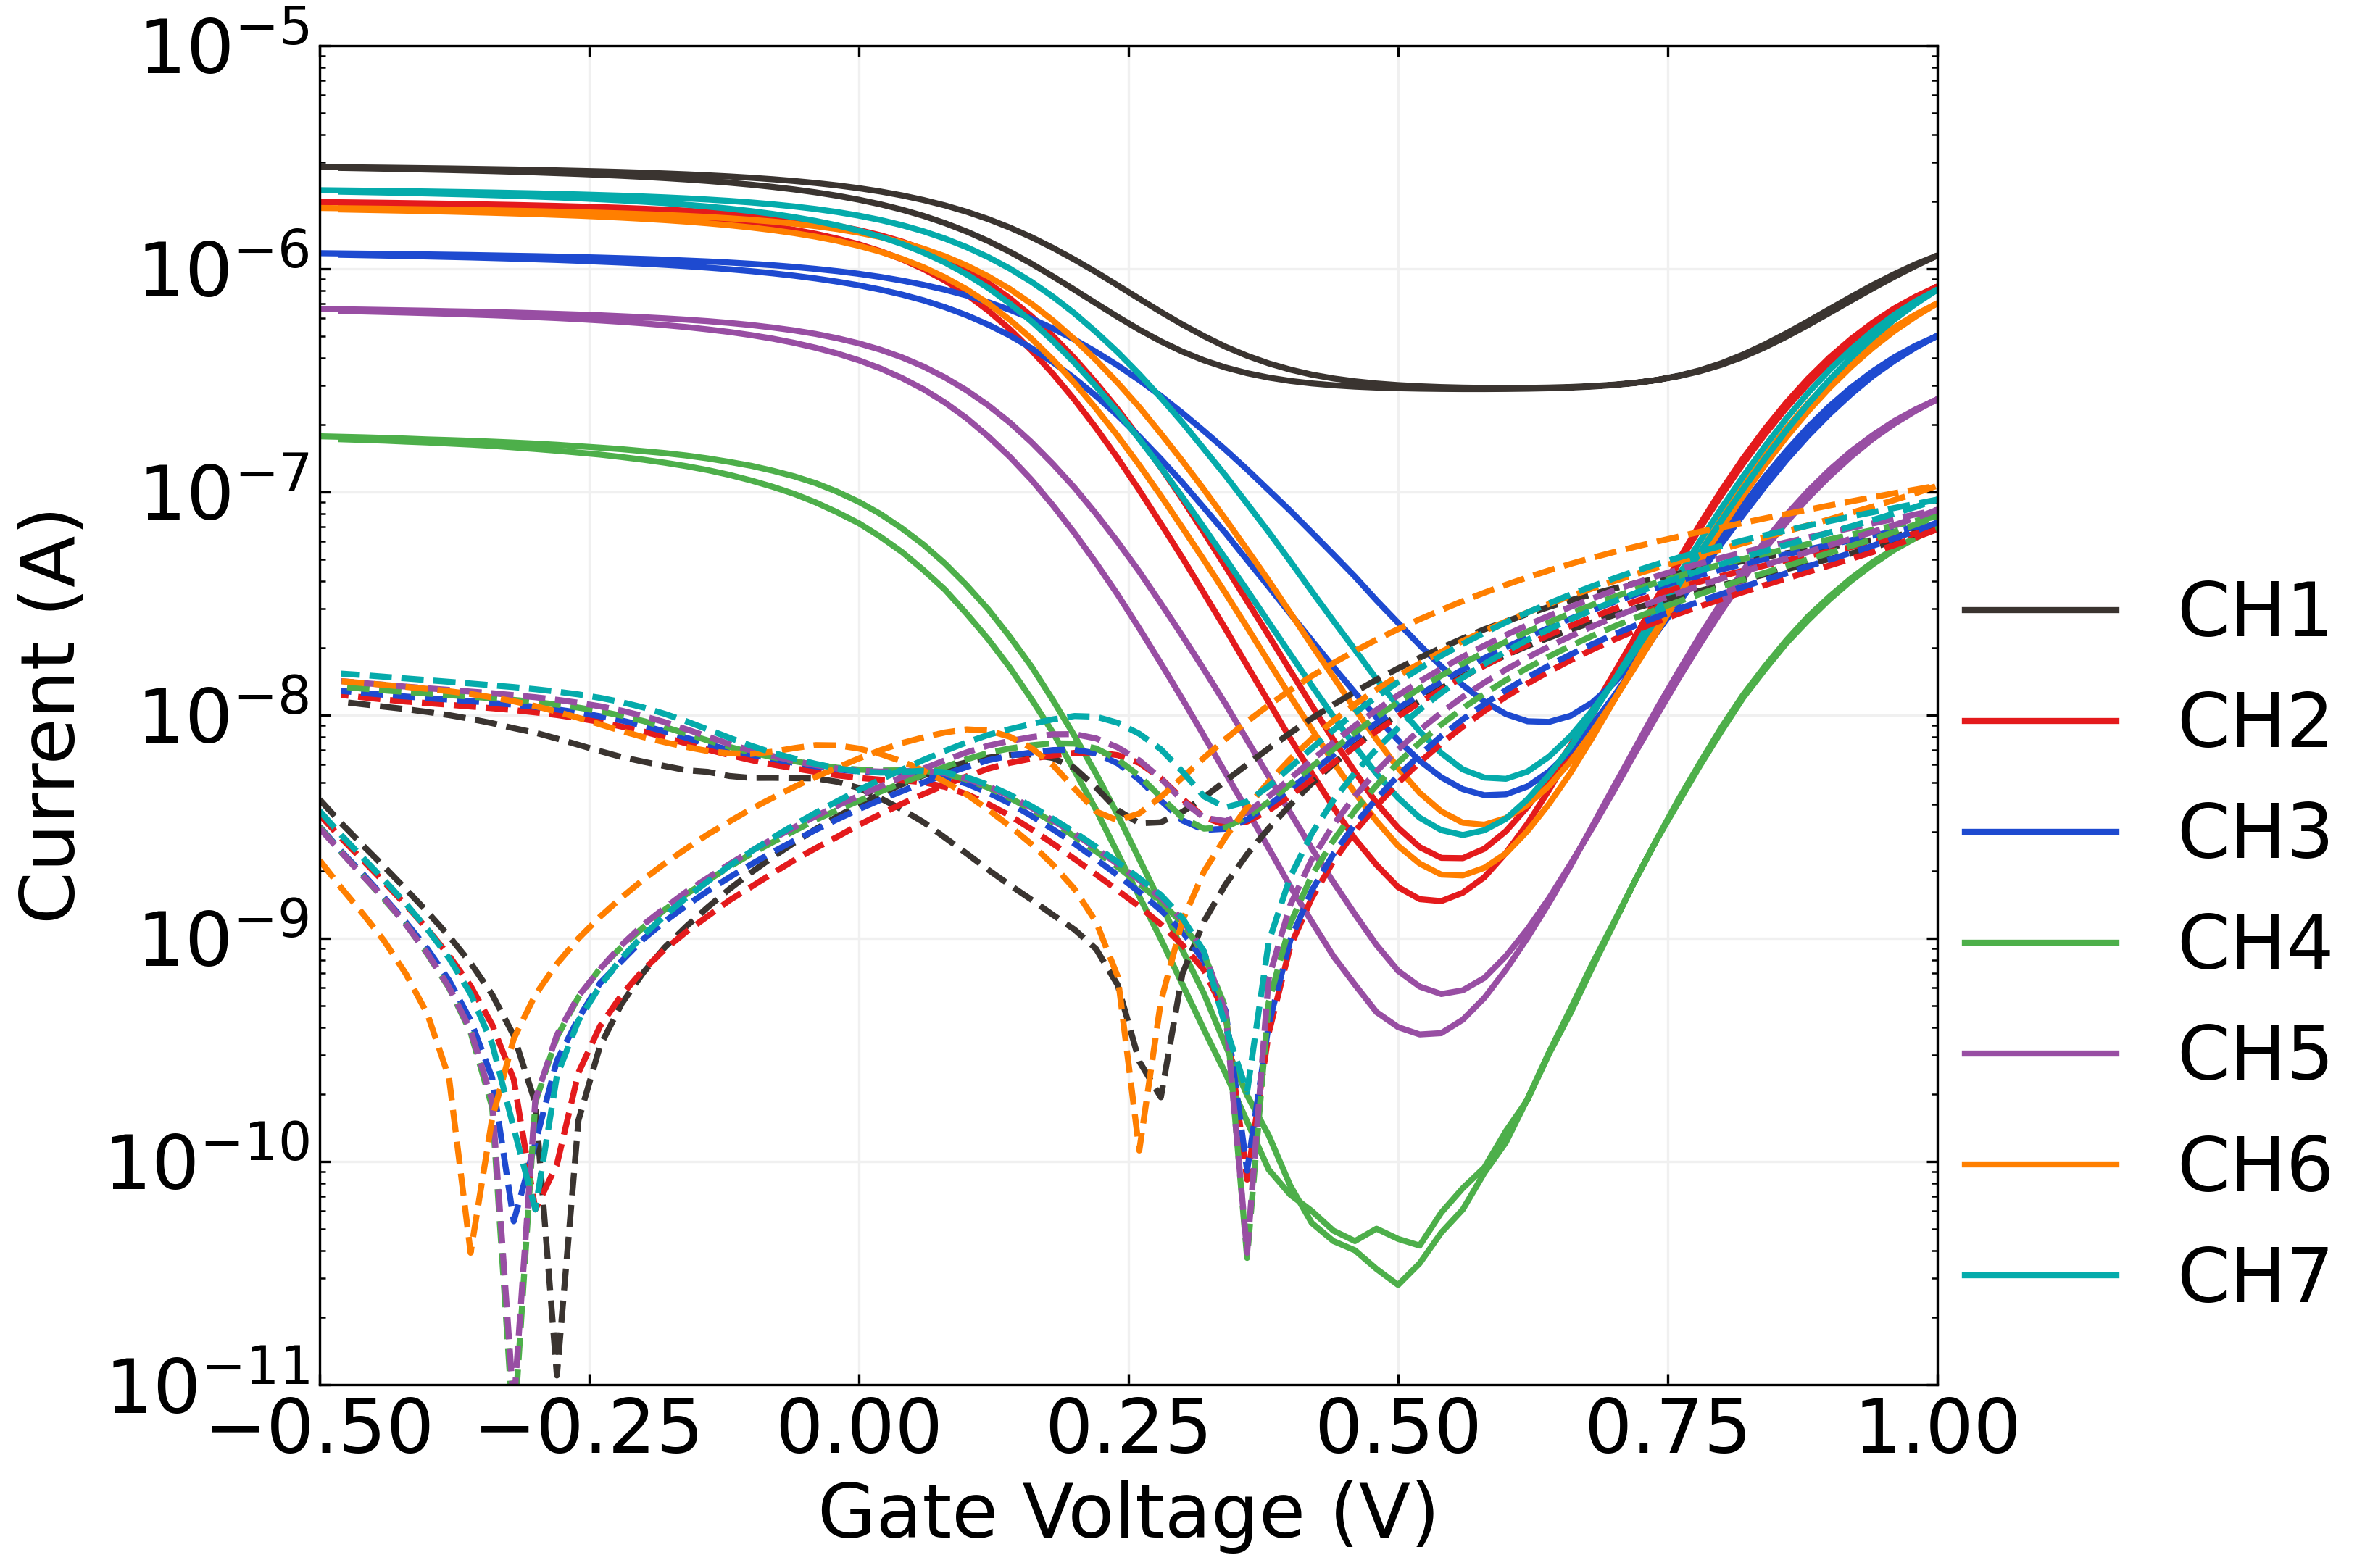
\includegraphics{figures/ch6/NTQ24C8_pristine_TXLG01_220211_solvent_gate.png}

}

}

\subcaption{\label{fig-solvent-tx-lg}}
\end{minipage}%
%
\begin{minipage}[t]{0.02\linewidth}

{\centering 

~

}

\end{minipage}%
%
\begin{minipage}[t]{0.49\linewidth}

{\centering 

\raisebox{-\height}{

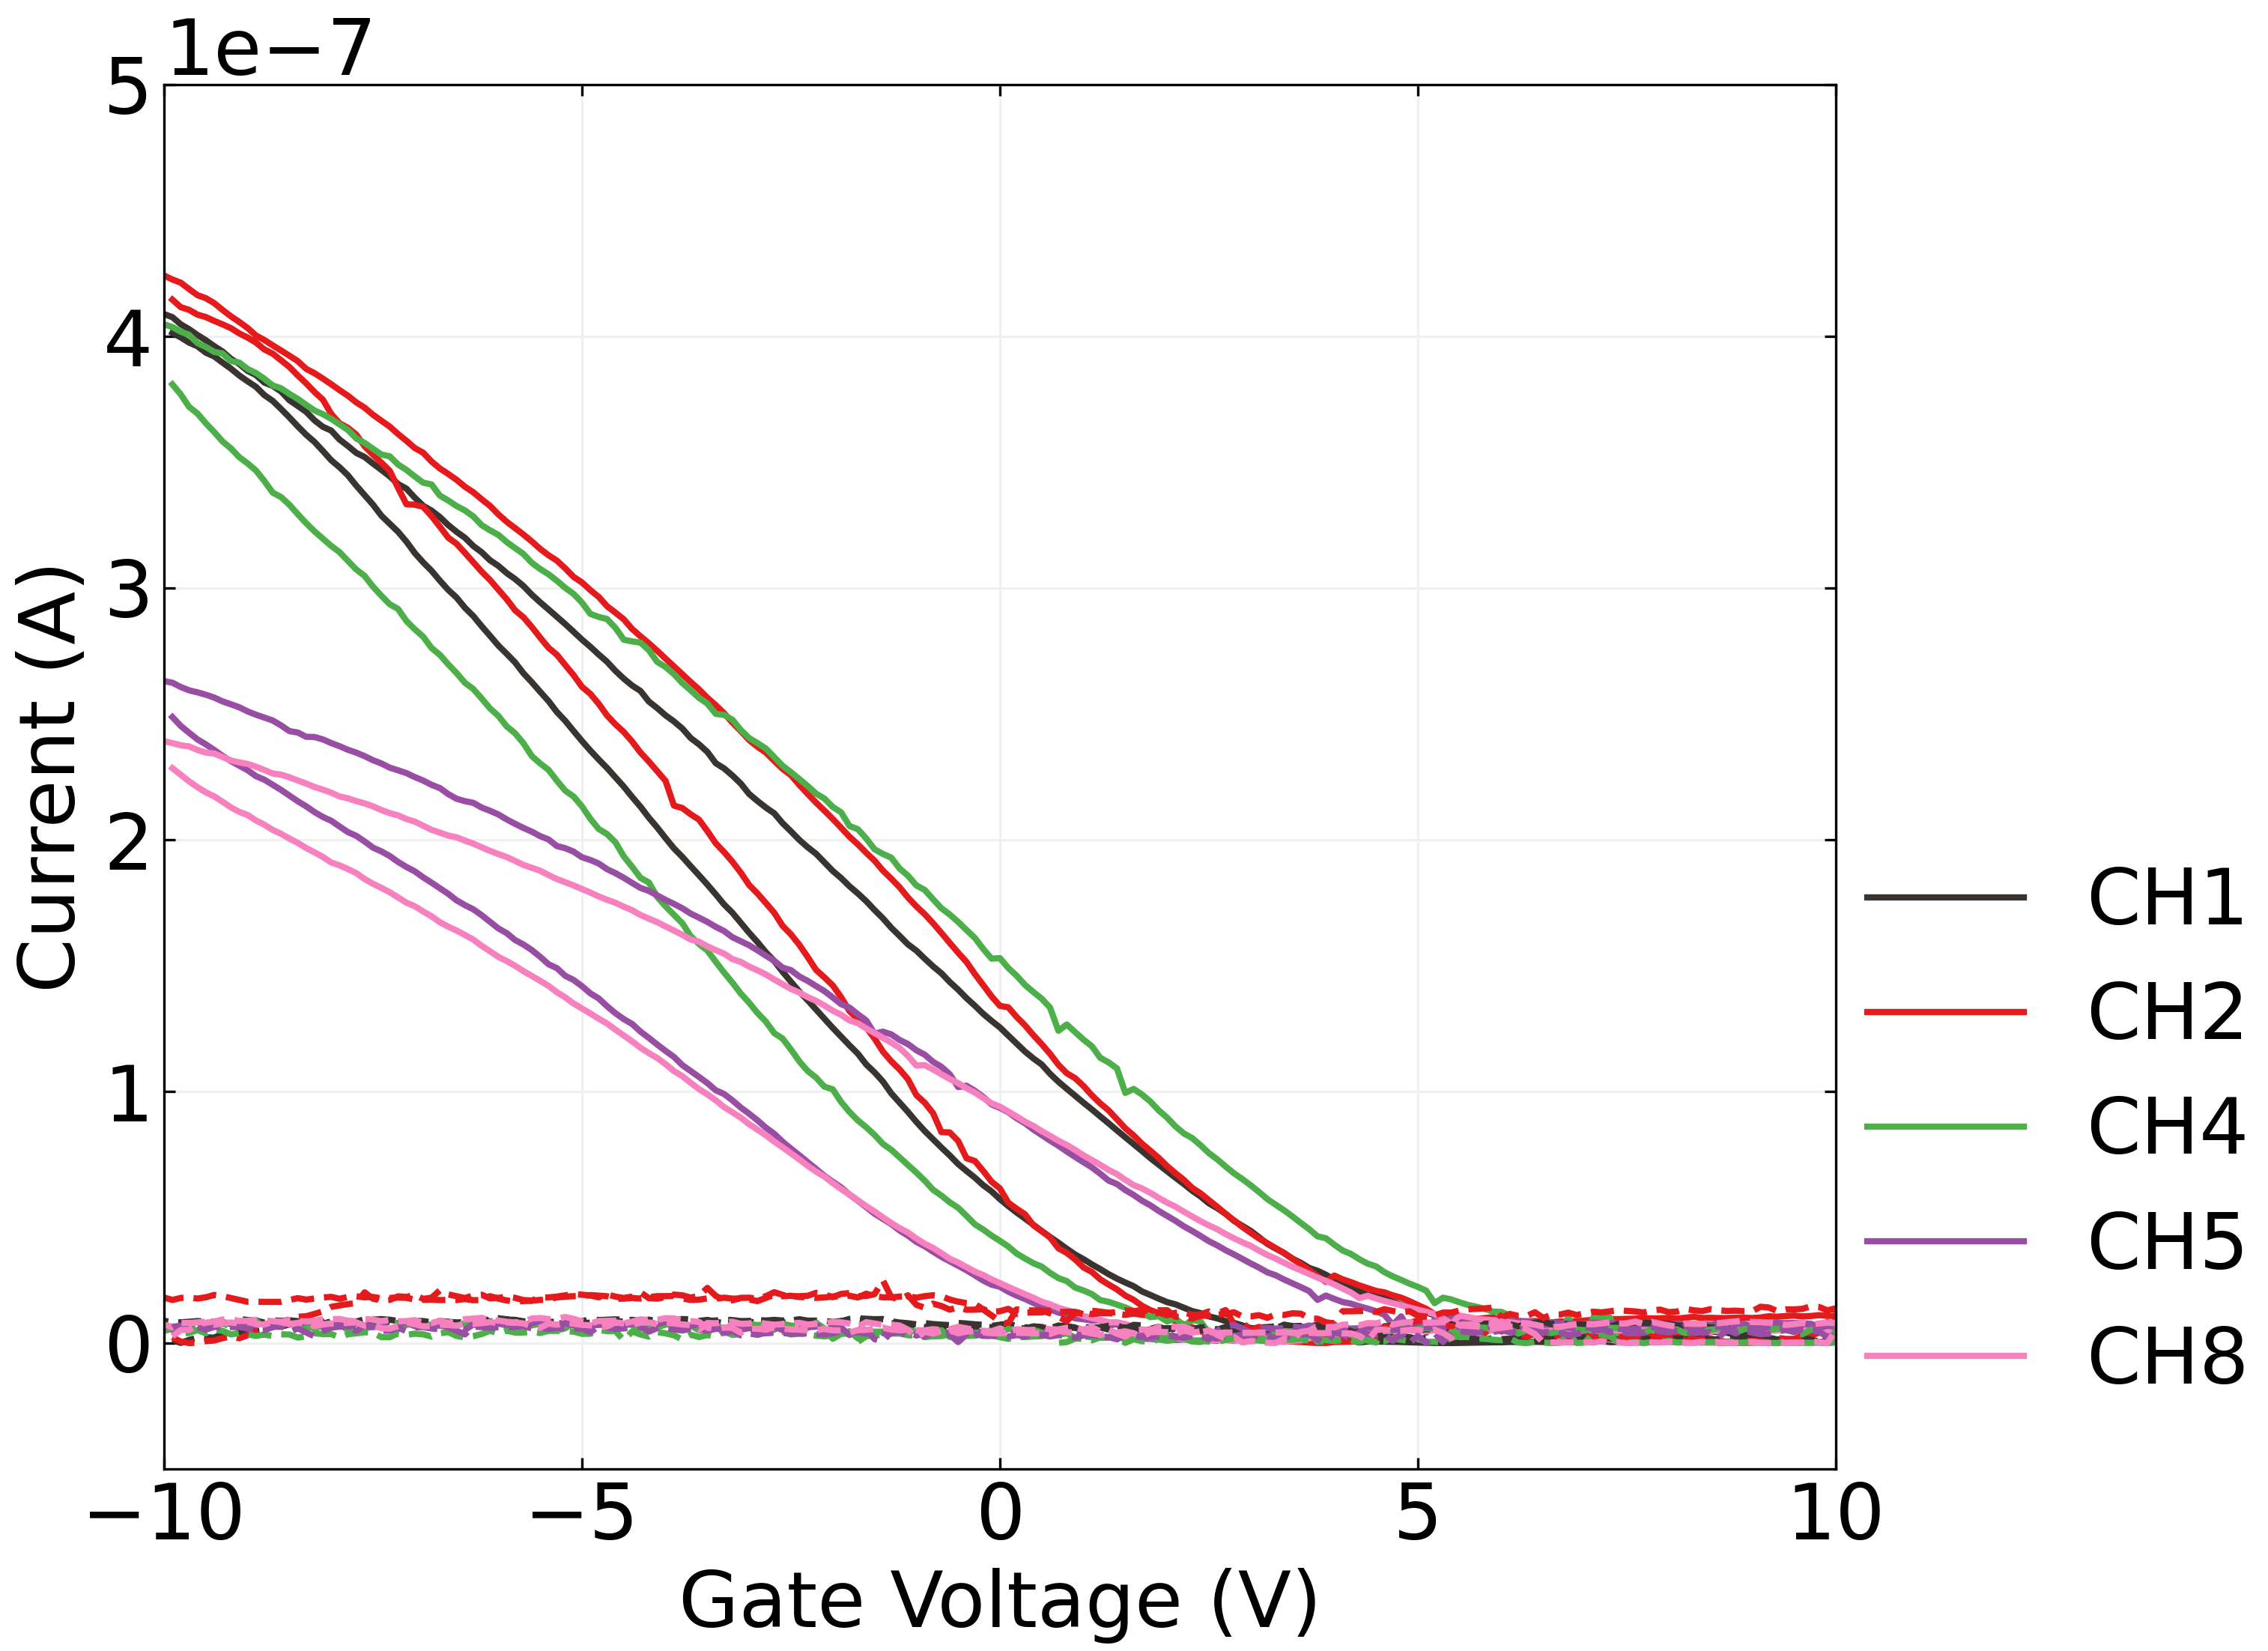
\includegraphics{figures/ch6/NTQ22C2_solvent_backgate.png}

}

}

\subcaption{\label{fig-solvent-tx-bg}}
\end{minipage}%
\newline
\begin{minipage}[t]{0.49\linewidth}

{\centering 

\raisebox{-\height}{

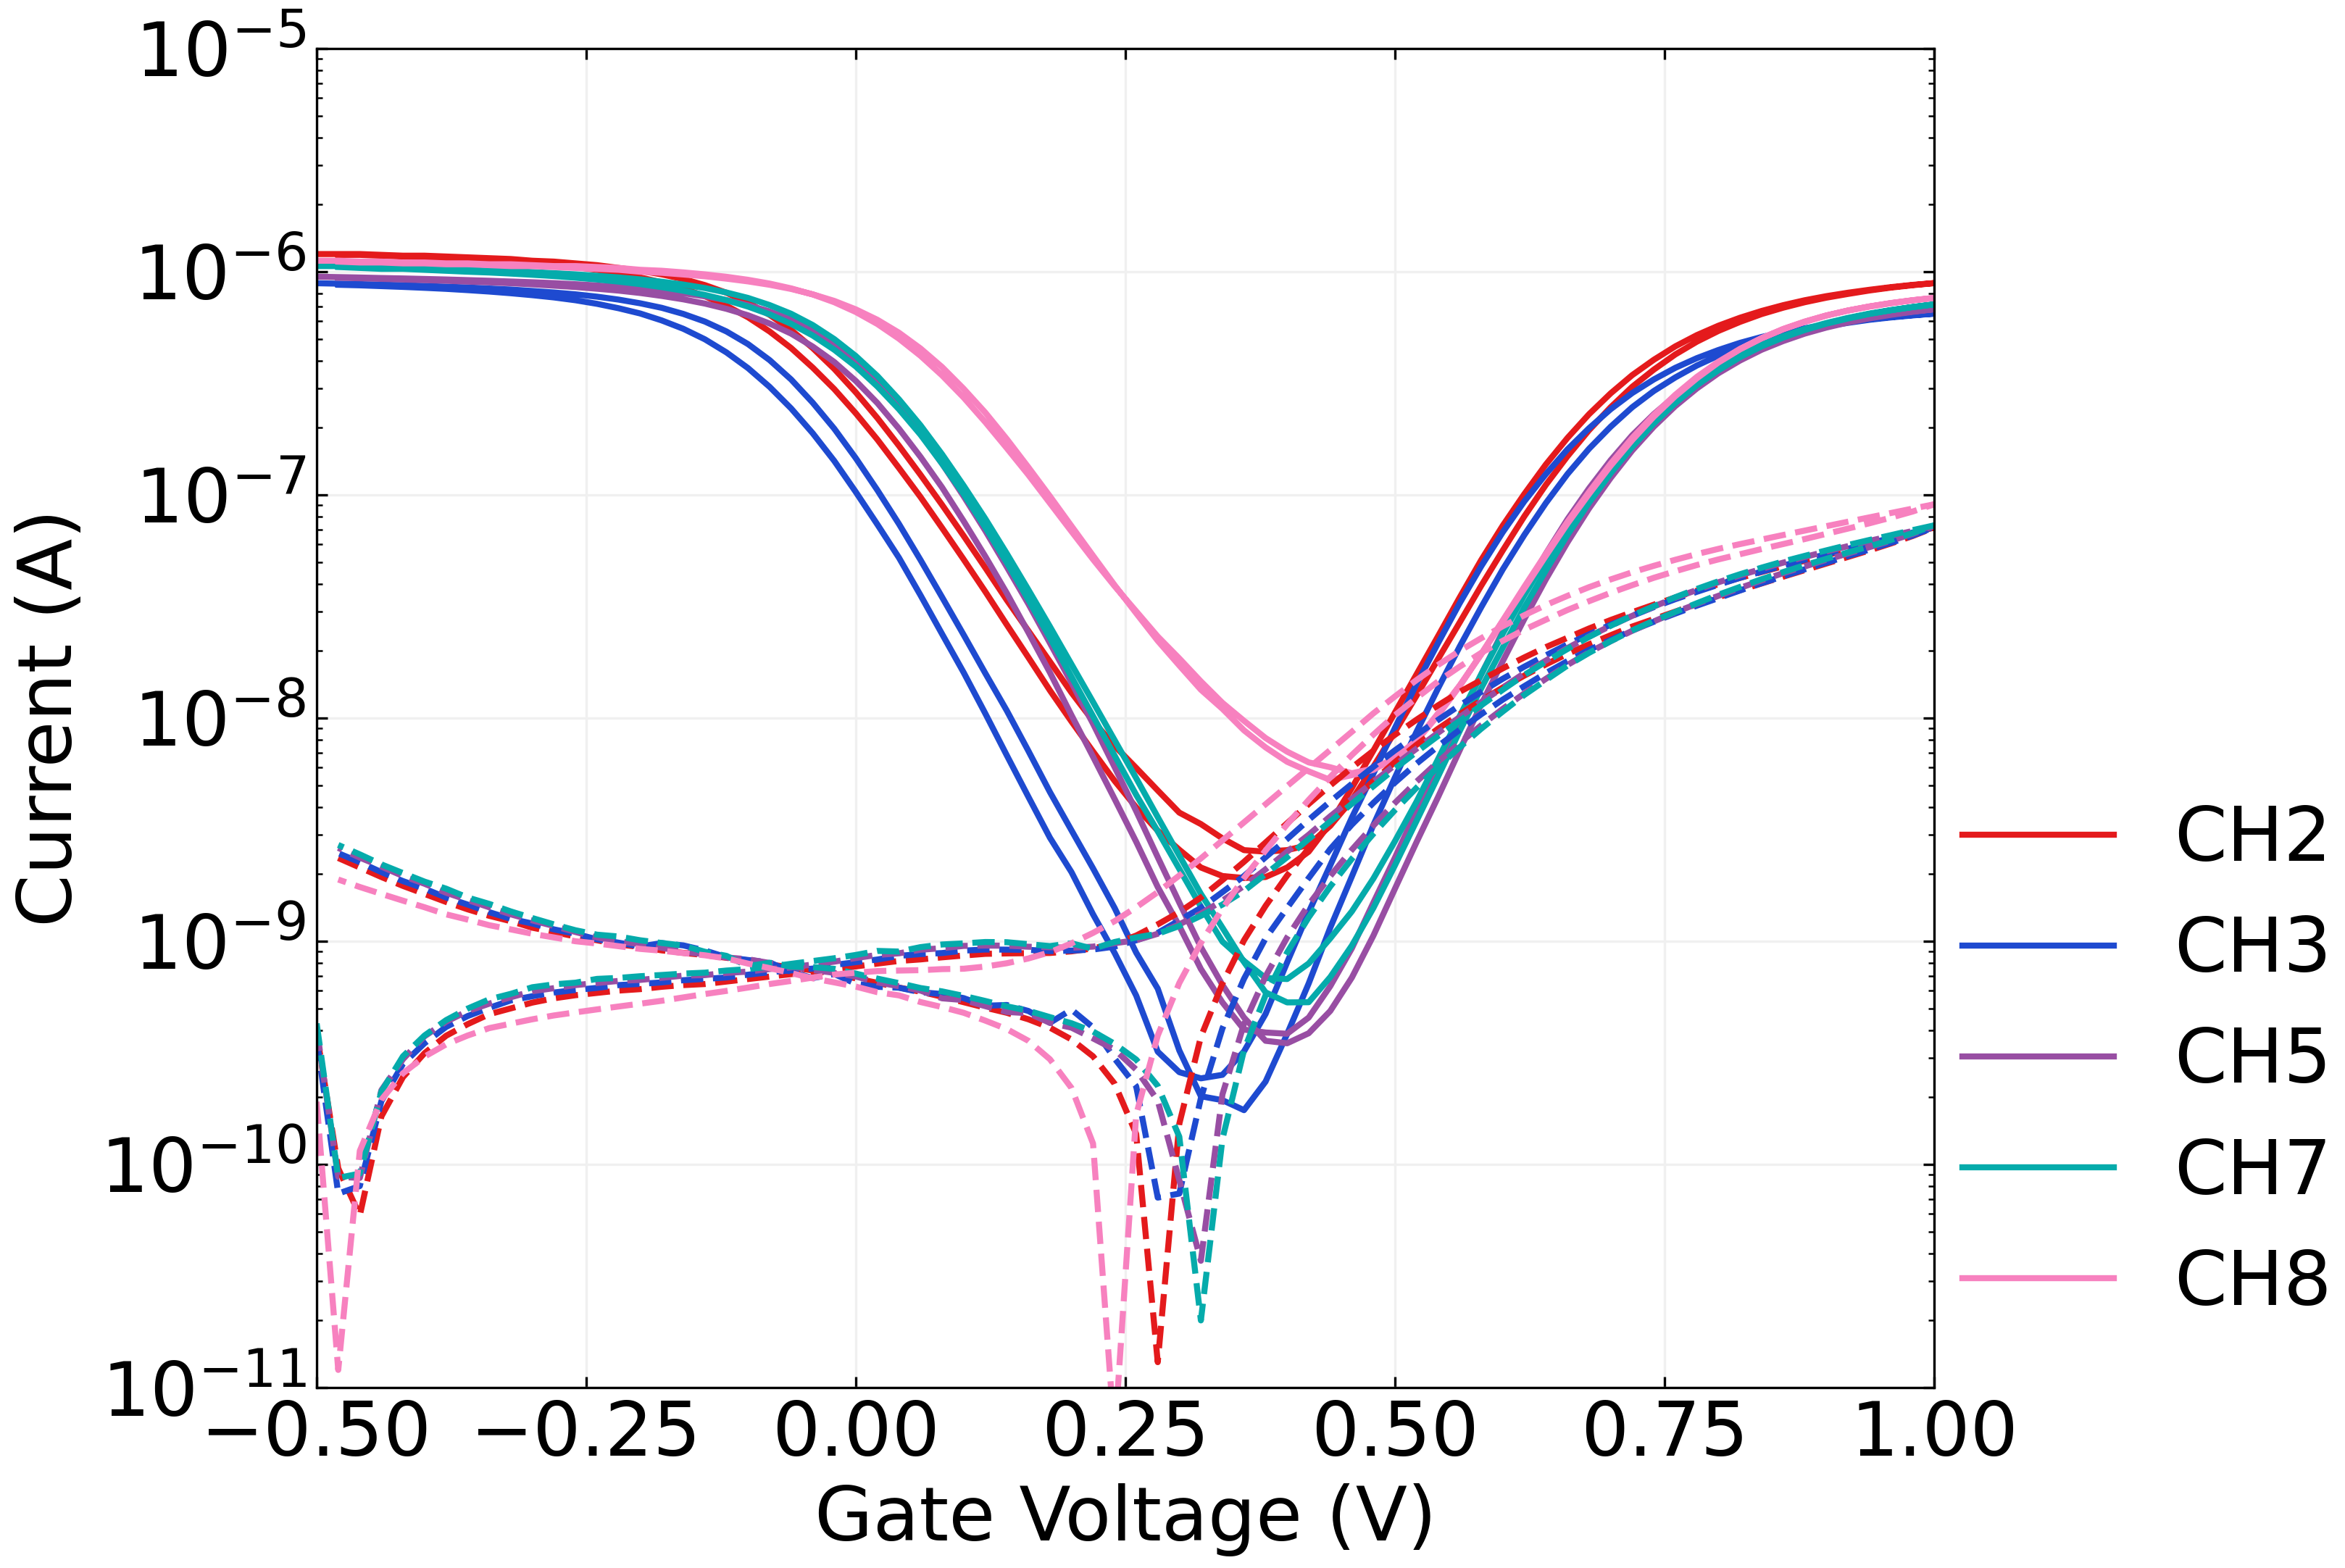
\includegraphics{figures/ch6/NTQ5C3_pristine_TXLG01_210602_nosteam_gate.png}

}

}

\subcaption{\label{fig-surf-tx-lg}}
\end{minipage}%
%
\begin{minipage}[t]{0.02\linewidth}

{\centering 

~

}

\end{minipage}%
%
\begin{minipage}[t]{0.49\linewidth}

{\centering 

\raisebox{-\height}{

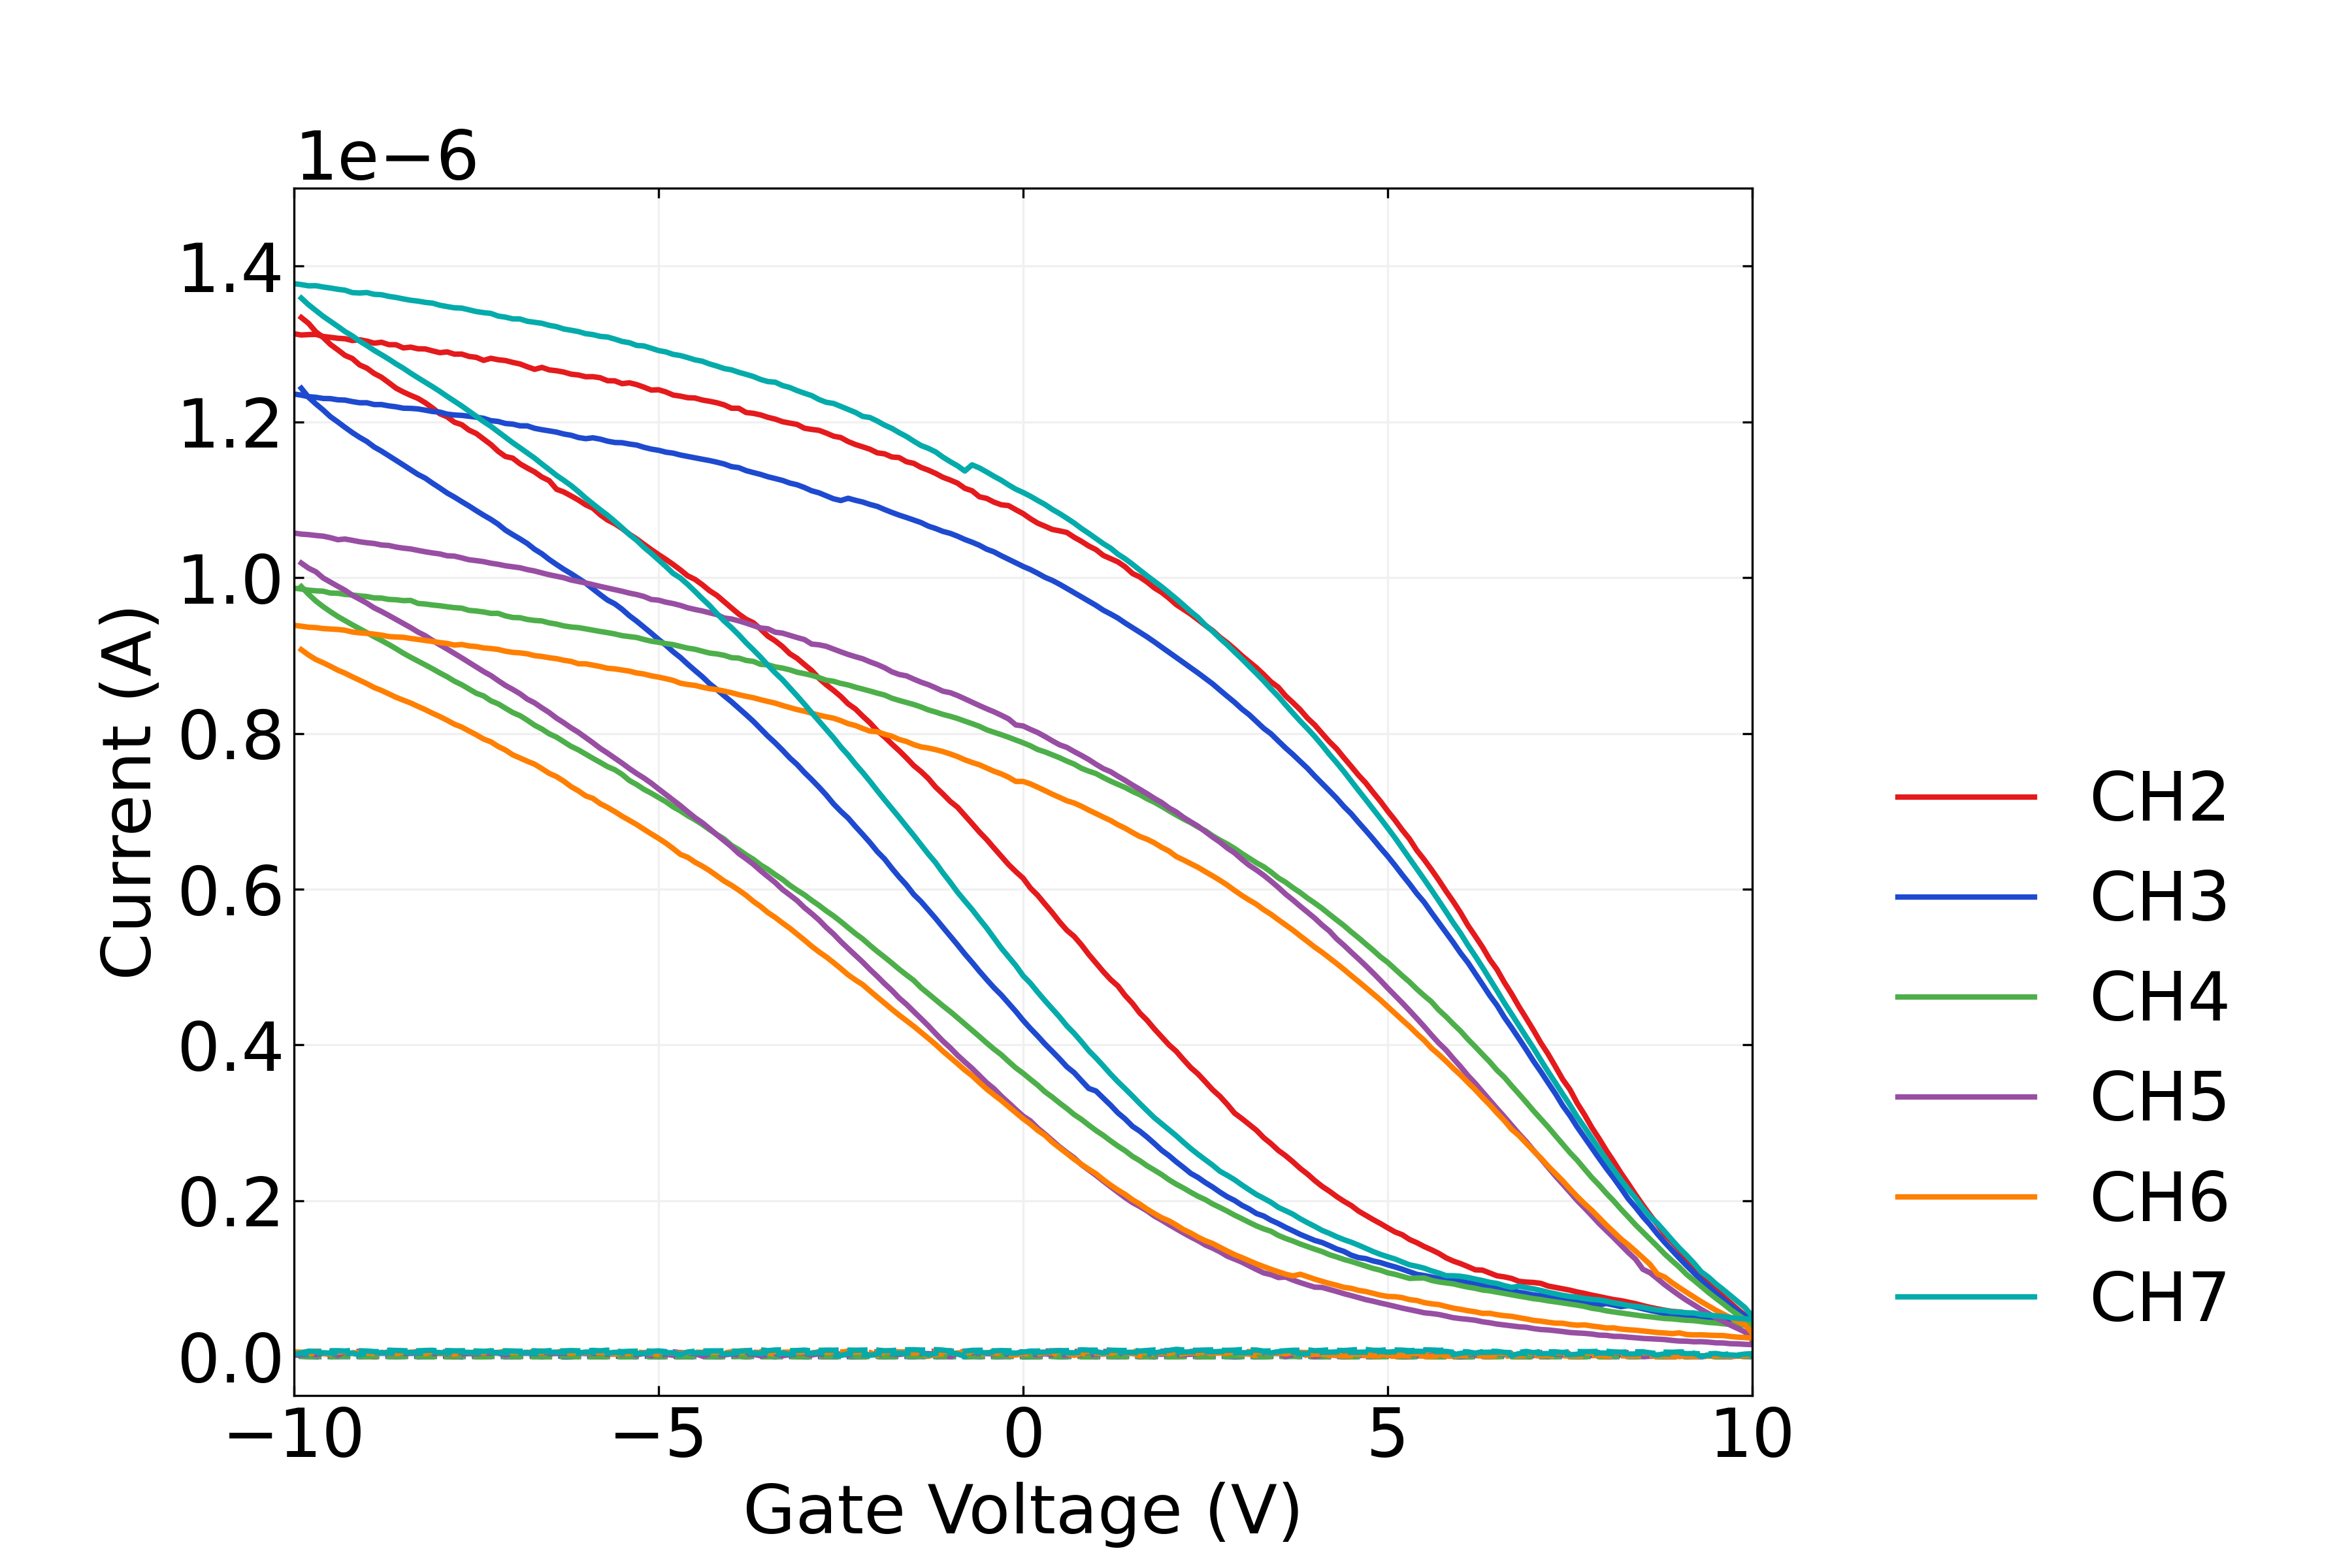
\includegraphics{figures/ch6/Q5C10_nosteam_backgate.png}

}

}

\subcaption{\label{fig-surf-tx-bg}}
\end{minipage}%
\newline
\begin{minipage}[t]{0.49\linewidth}

{\centering 

\raisebox{-\height}{

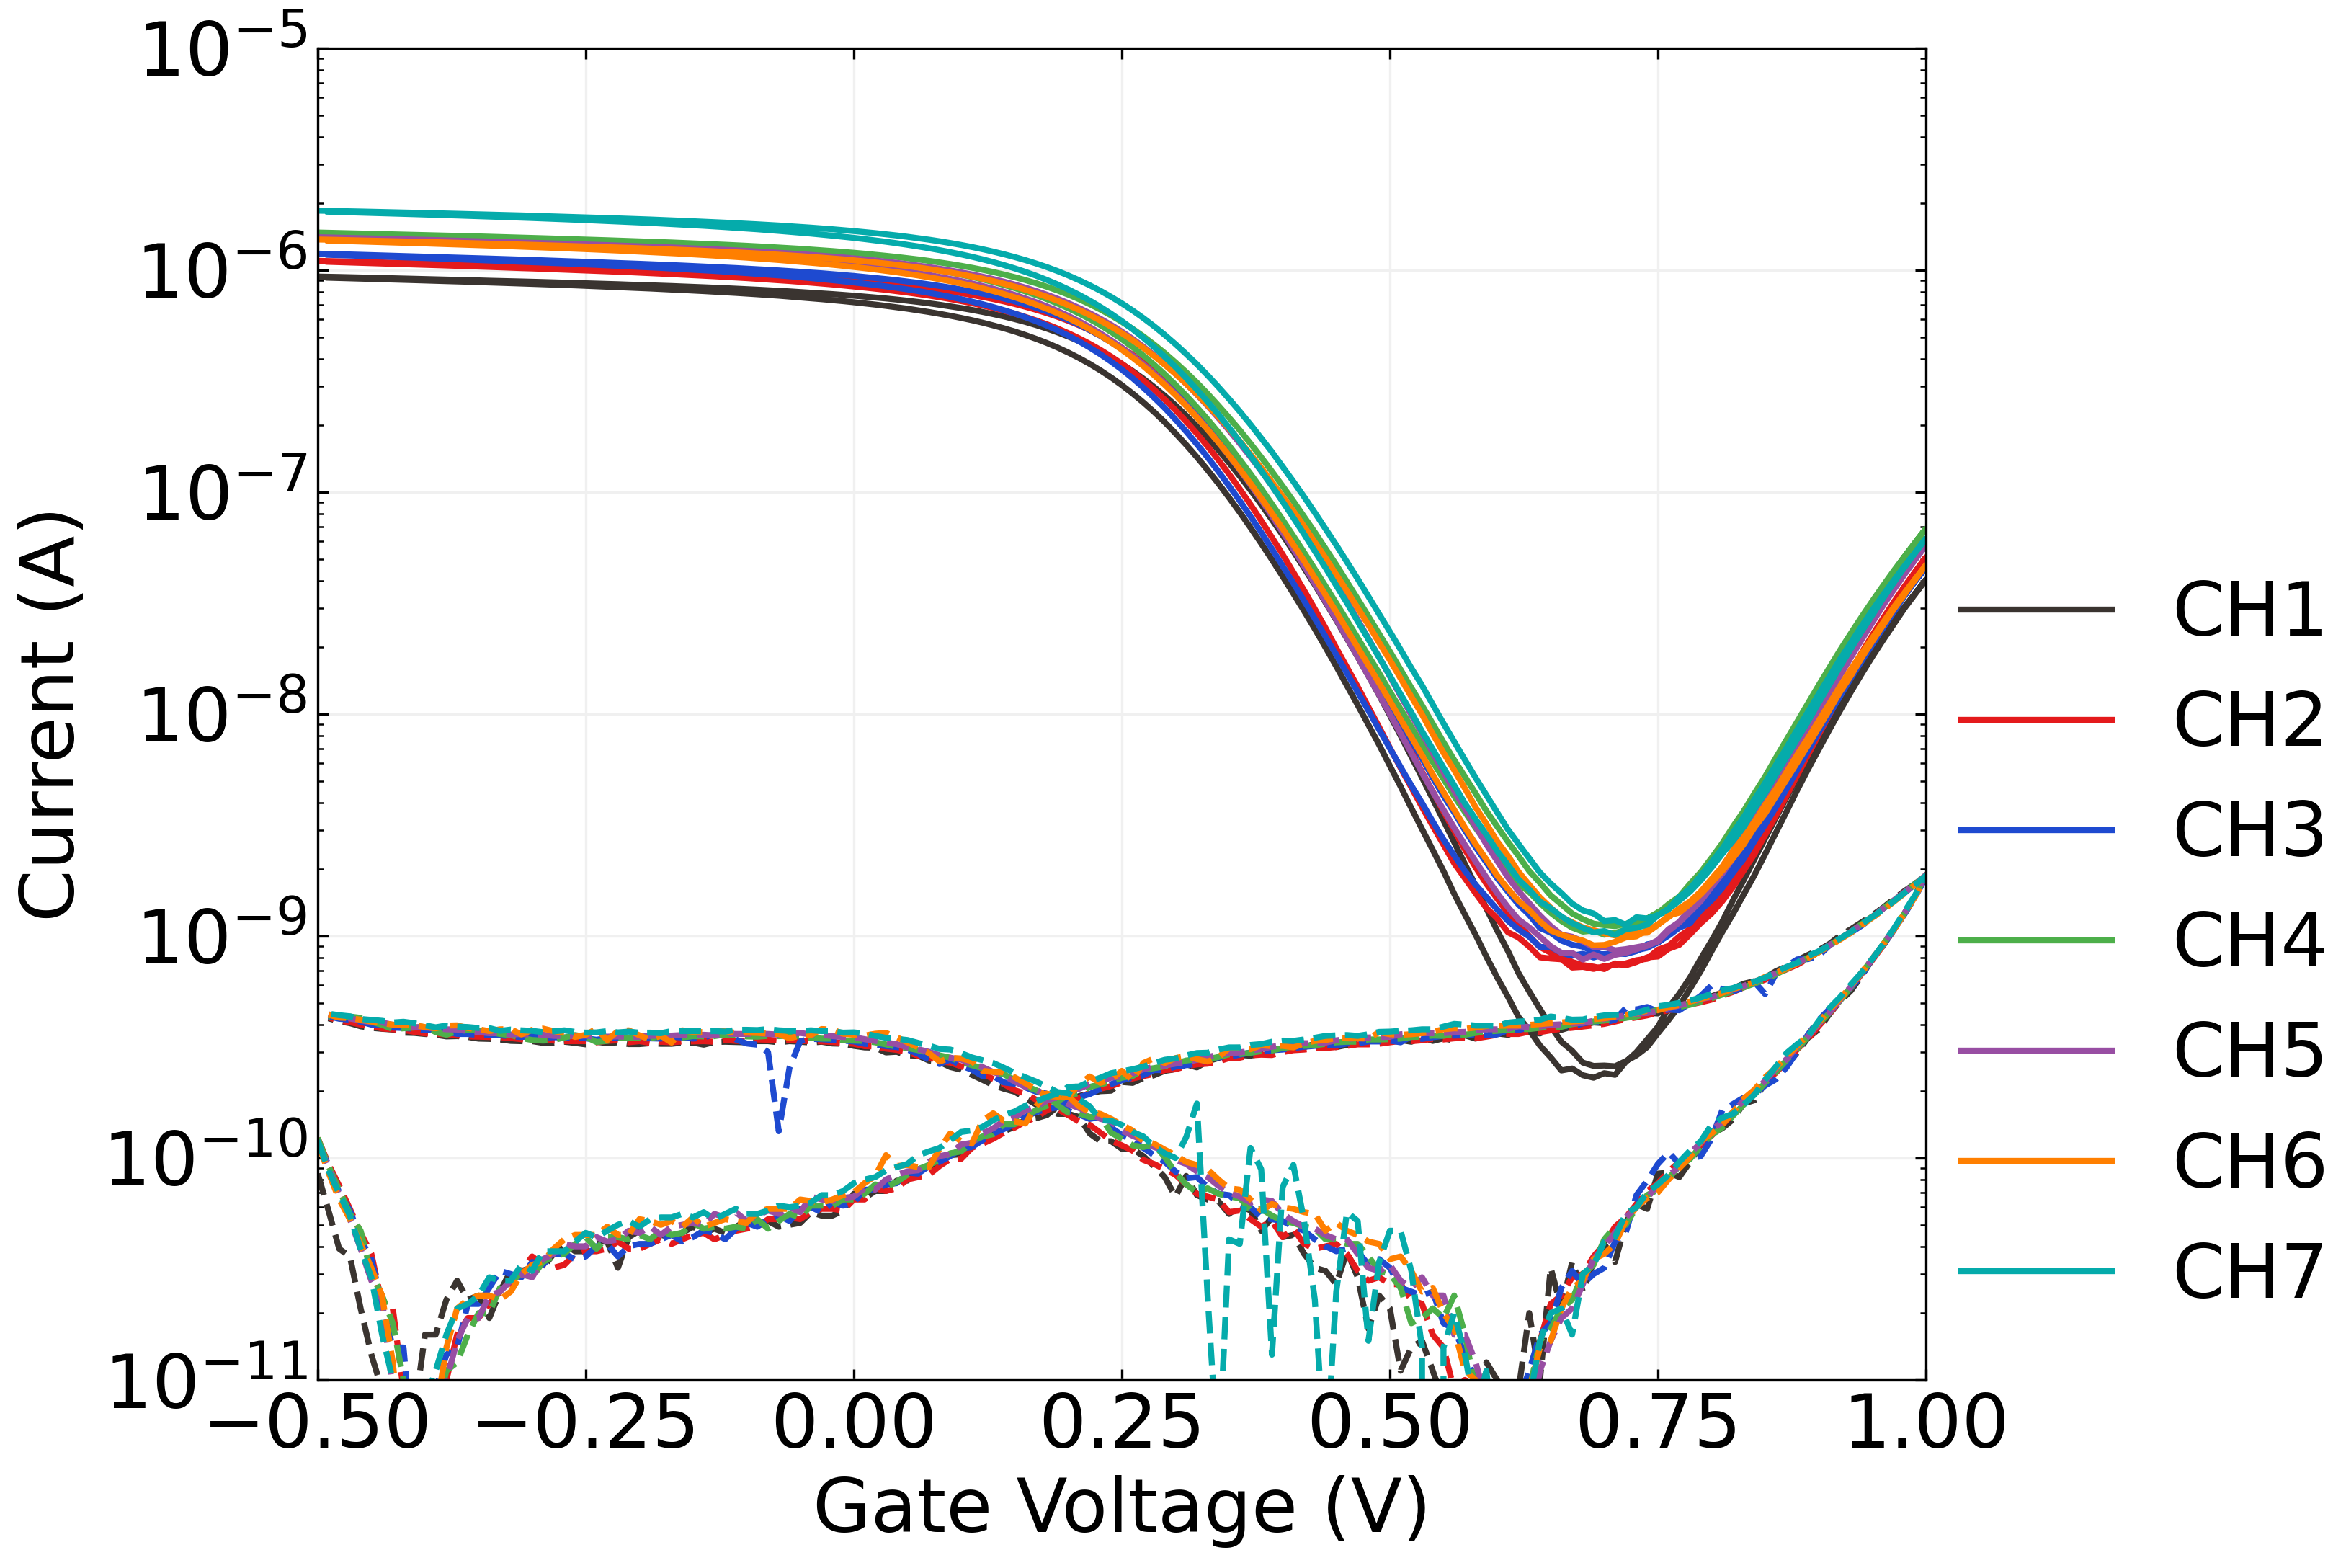
\includegraphics{figures/ch6/NTQ31C6_pristine_TXLG01_230330_steam_gate.png}

}

}

\subcaption{\label{fig-steam-tx-lg}}
\end{minipage}%
%
\begin{minipage}[t]{0.02\linewidth}

{\centering 

~

}

\end{minipage}%
%
\begin{minipage}[t]{0.49\linewidth}

{\centering 

\raisebox{-\height}{

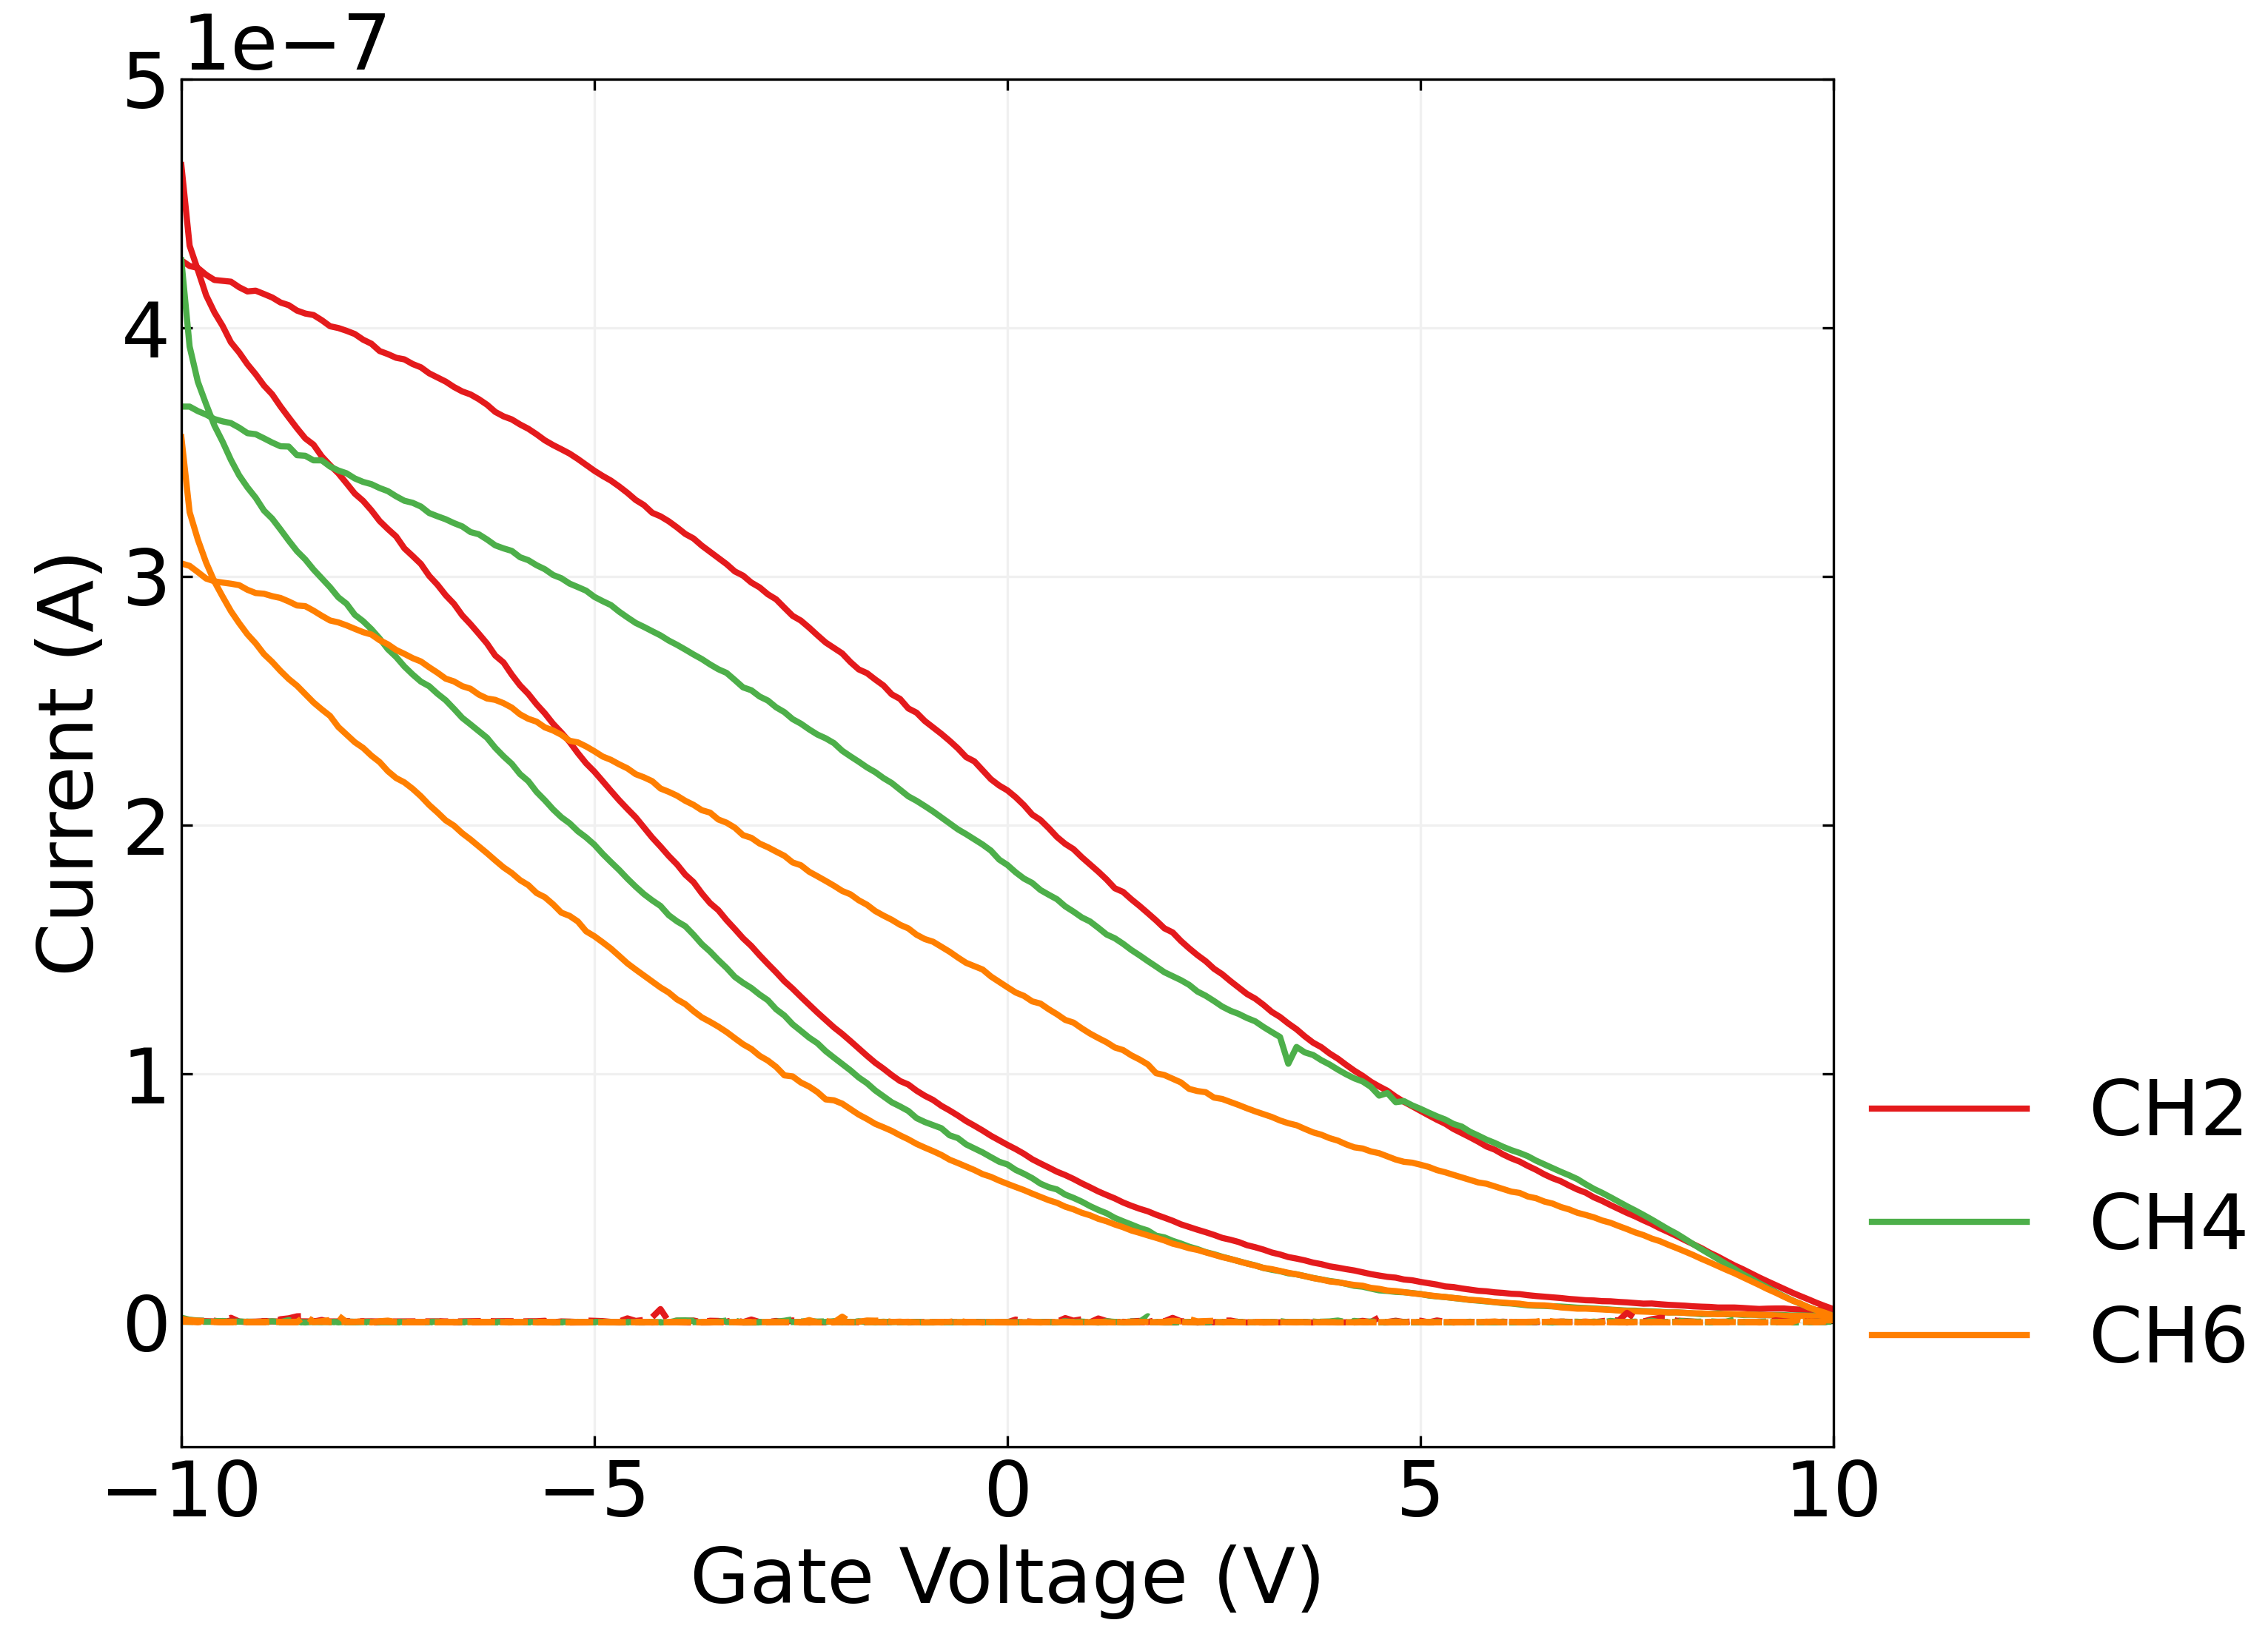
\includegraphics{figures/ch6/Q18C6_steam_backgate.png}

}

}

\subcaption{\label{fig-steam-tx-bg}}
\end{minipage}%

\caption{\label{fig-pristine-cnt-characteristics}Liquid-gated (left) and
back-gated (right) transfer characteristics of AZ\(^\circledR\) 1518
encapsulated field-effect transistors, where the film was deposited with
solvent in (a) and (b), deposited with surfactant in (c) and (d), and
deposited with surfactant in the presence of steam in (e) and (f). A
step size of 100 mV was used for the backgated sweeps in (a), (c) and
(e), while a step size of 20 mV was used for the liquid-gated sweeps in
(b), (d) and (f). Gate current (leakage current) is shown with a dashed
line. The source-drain voltage used for all sweeps was
\(V_{ds} = 100 \textrm{mV}\), and 1XPBS was used as the buffer for the
liquid-gated measurements here.}

\end{figure}

Each carbon nanotube device fabricated was electrically characterised as
described in \textbf{?@sec-electrical-characterisation}, and electrical
data was analysed using the Python code discussed in
Section~\ref{sec-field-effect-transistor-analysis}. Devices with a 100
nm or 300 nm SiO\(_2\) layer were used for liquid gated measurements,
and devices with a 100 nm SiO\(_2\) layer were used for backgated
measurements. Figure~\ref{fig-pristine-cnt-characteristics} displays
multi-channel measurements of representative devices fabricated as
described in \textbf{?@sec-fabrication}. To ensure a consistent
comparison, each device here was encapsulated with AZ\(^\circledR\) 1518
encapsulation before measurements were taken. The channels which did not
exhibit reliable transistor characteristics are not shown. These
`non-working' channels were either shorted, due to metal remaining on
the channel after lift-off, or were very low current, due to a very
sparse carbon nanotube network. Devices shown here with a
solvent-deposited carbon nanotube network were fabricated prior to Jan
2022; devices with a surfactant-deposited network without steam present
were fabricated prior to Jun 2021; devices with a surfactant-deposited
network without steam were fabricated prior to Sep 2022.

\begin{figure}

\begin{minipage}[t]{0.47\linewidth}

{\centering 

\raisebox{-\height}{

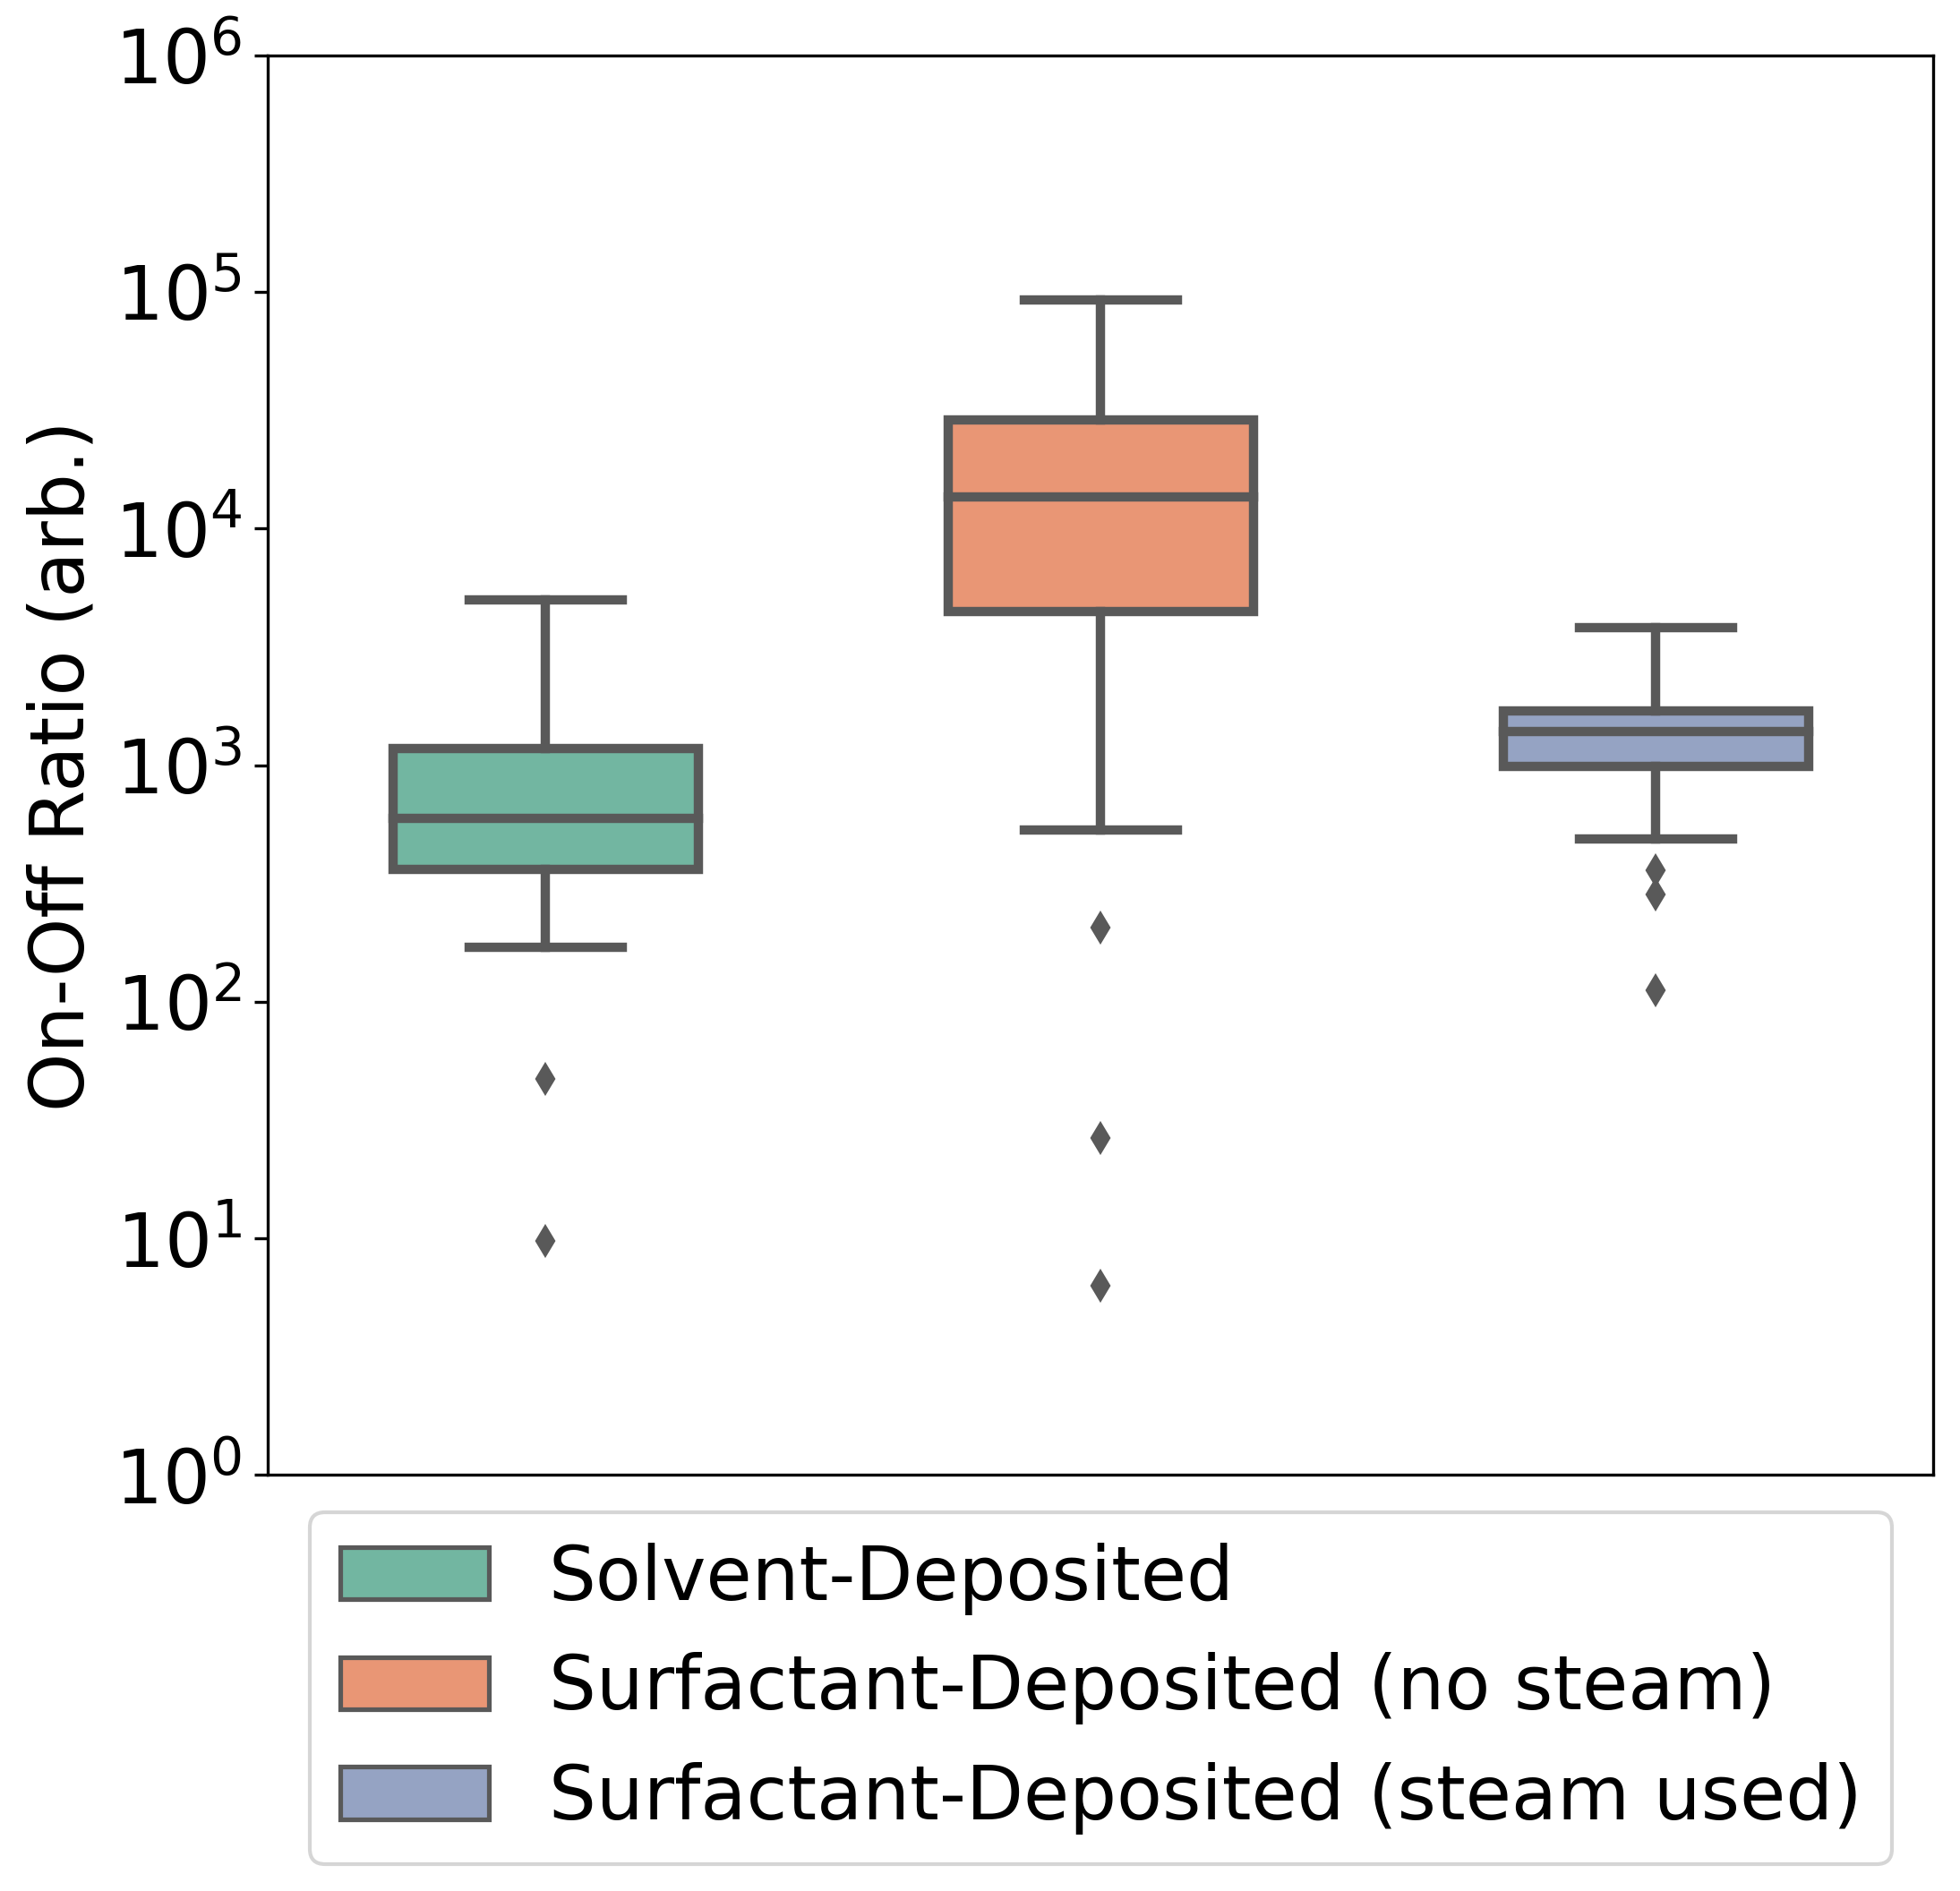
\includegraphics{figures/ch6/onoff_CNT.png}

}

}

\subcaption{\label{fig-on-off-ratio}}
\end{minipage}%
%
\begin{minipage}[t]{0.05\linewidth}

{\centering 

~

}

\end{minipage}%
%
\begin{minipage}[t]{0.47\linewidth}

{\centering 

\raisebox{-\height}{

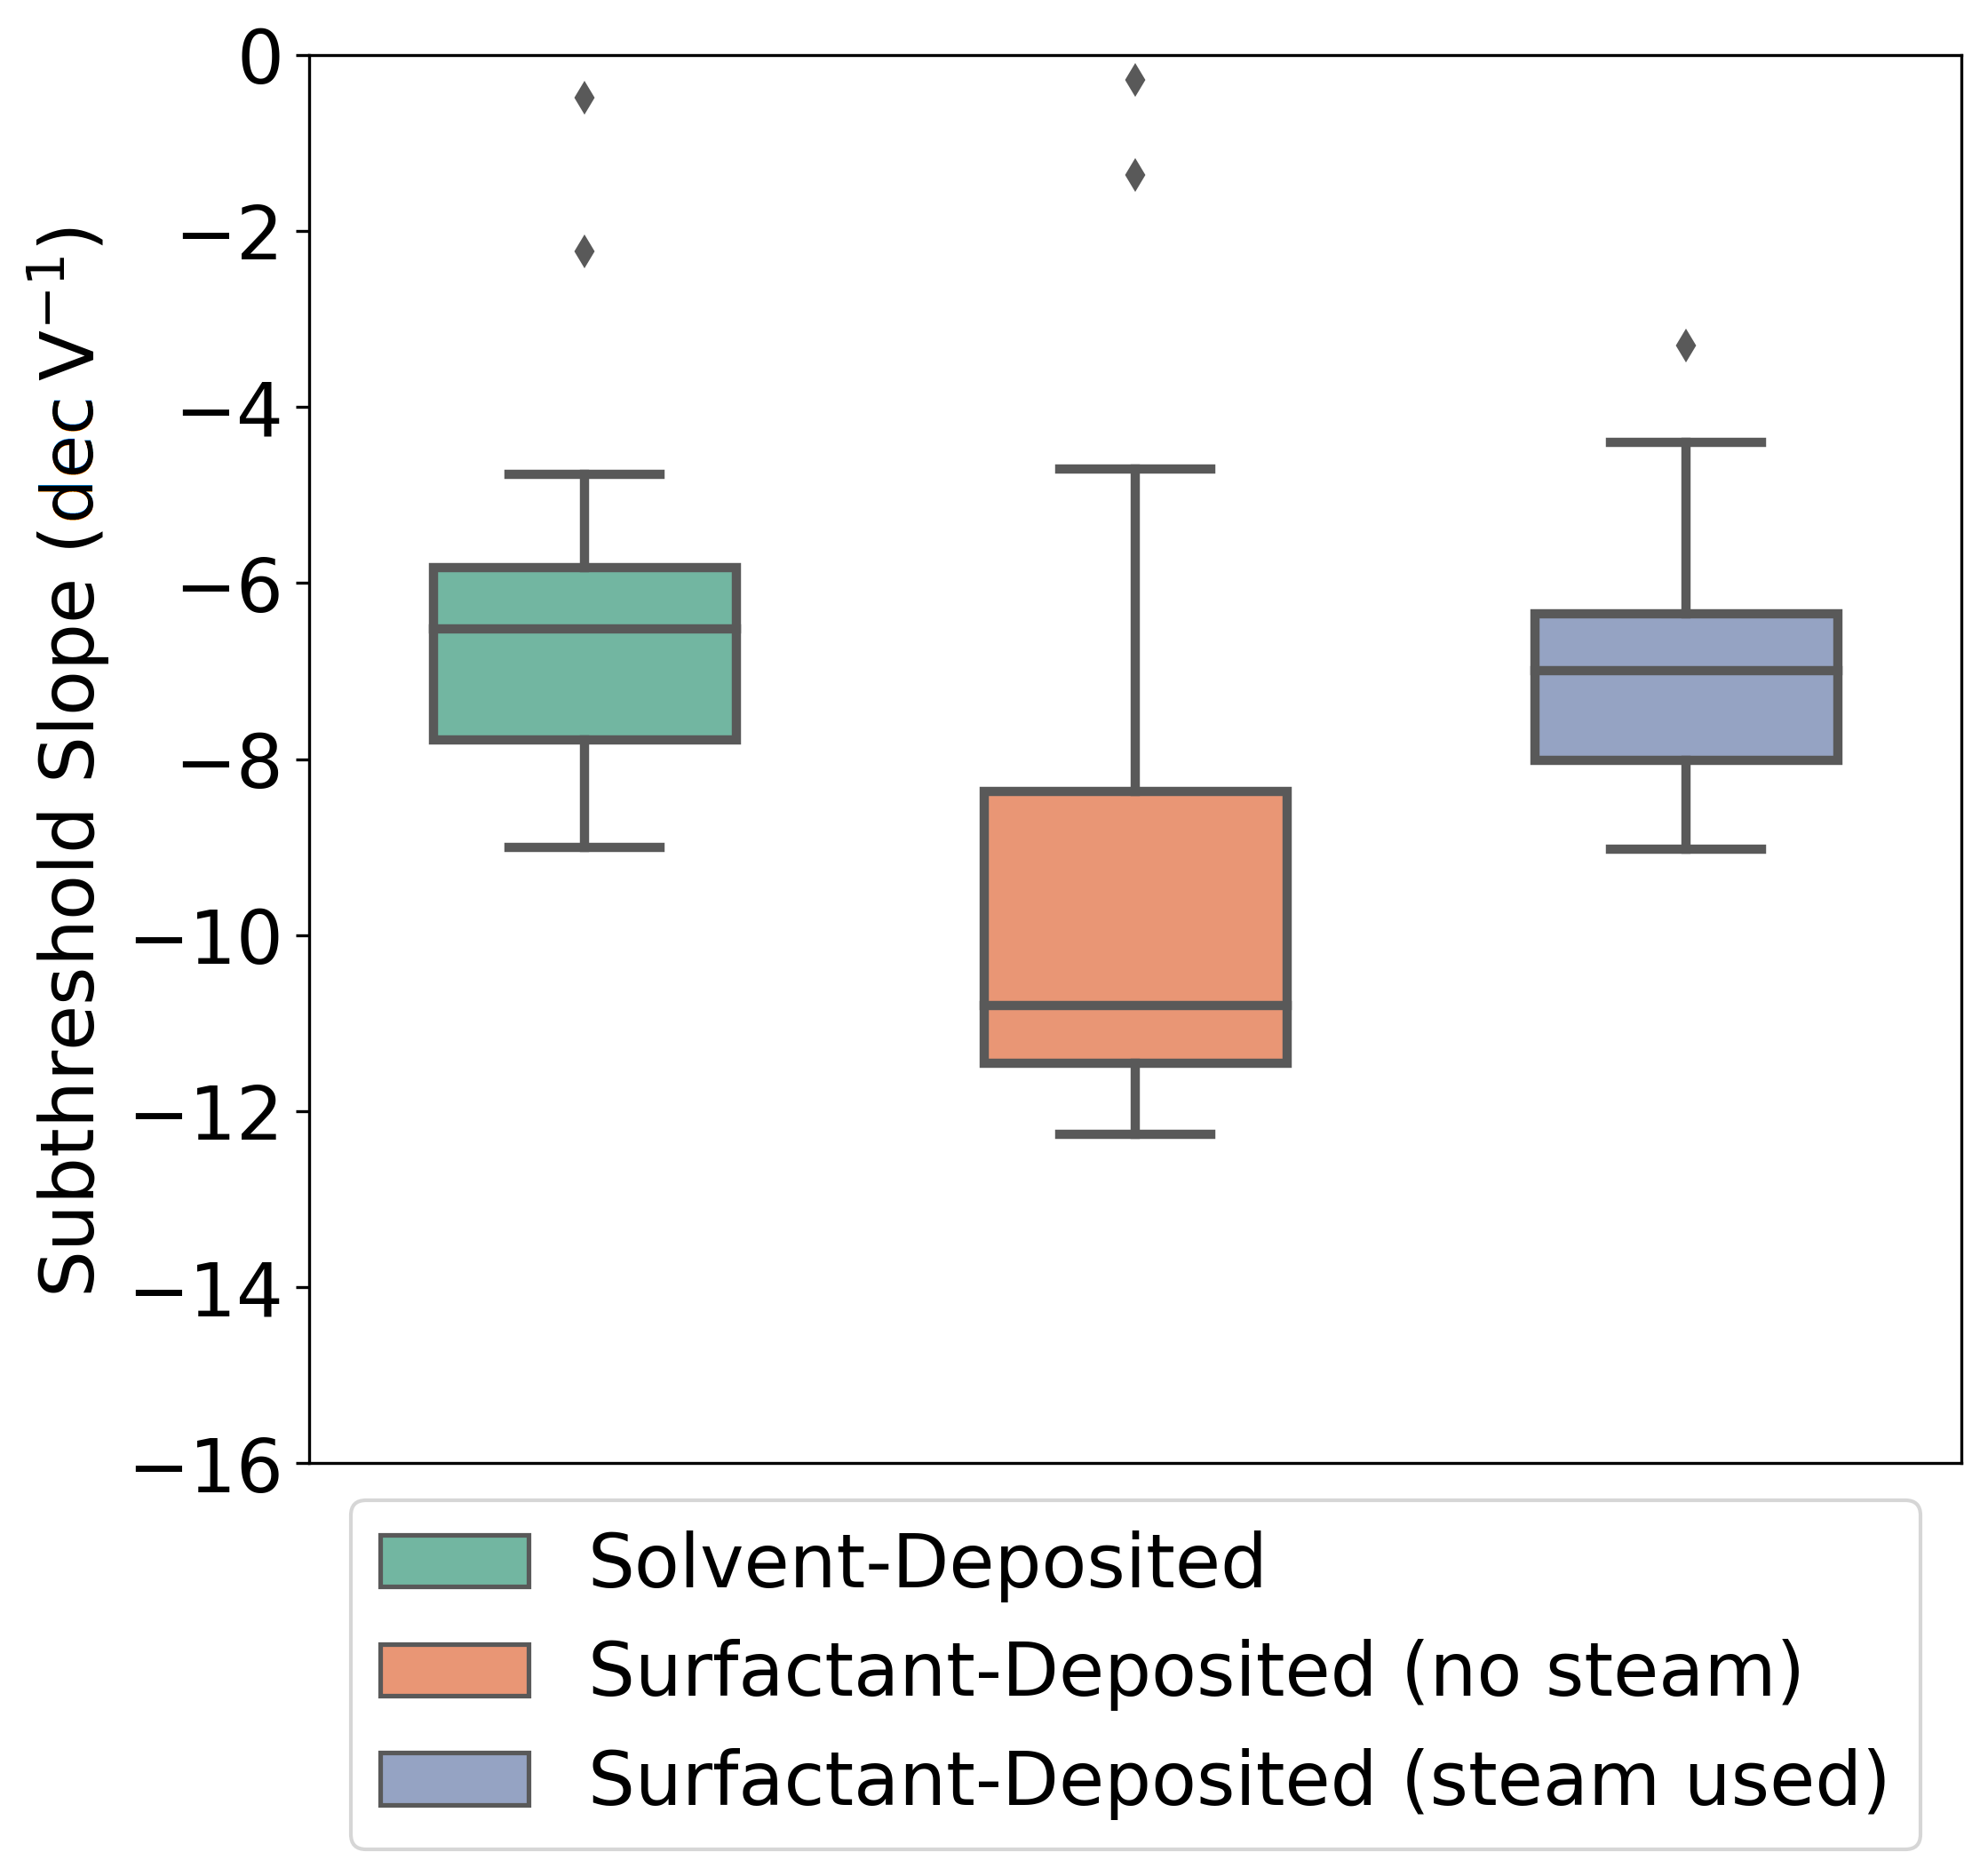
\includegraphics{figures/ch6/SS.png}

}

}

\subcaption{\label{fig-subthreshold-slope}}
\end{minipage}%
\newline
\begin{minipage}[t]{0.26\linewidth}

{\centering 

~

}

\end{minipage}%
%
\begin{minipage}[t]{0.47\linewidth}

{\centering 

\raisebox{-\height}{

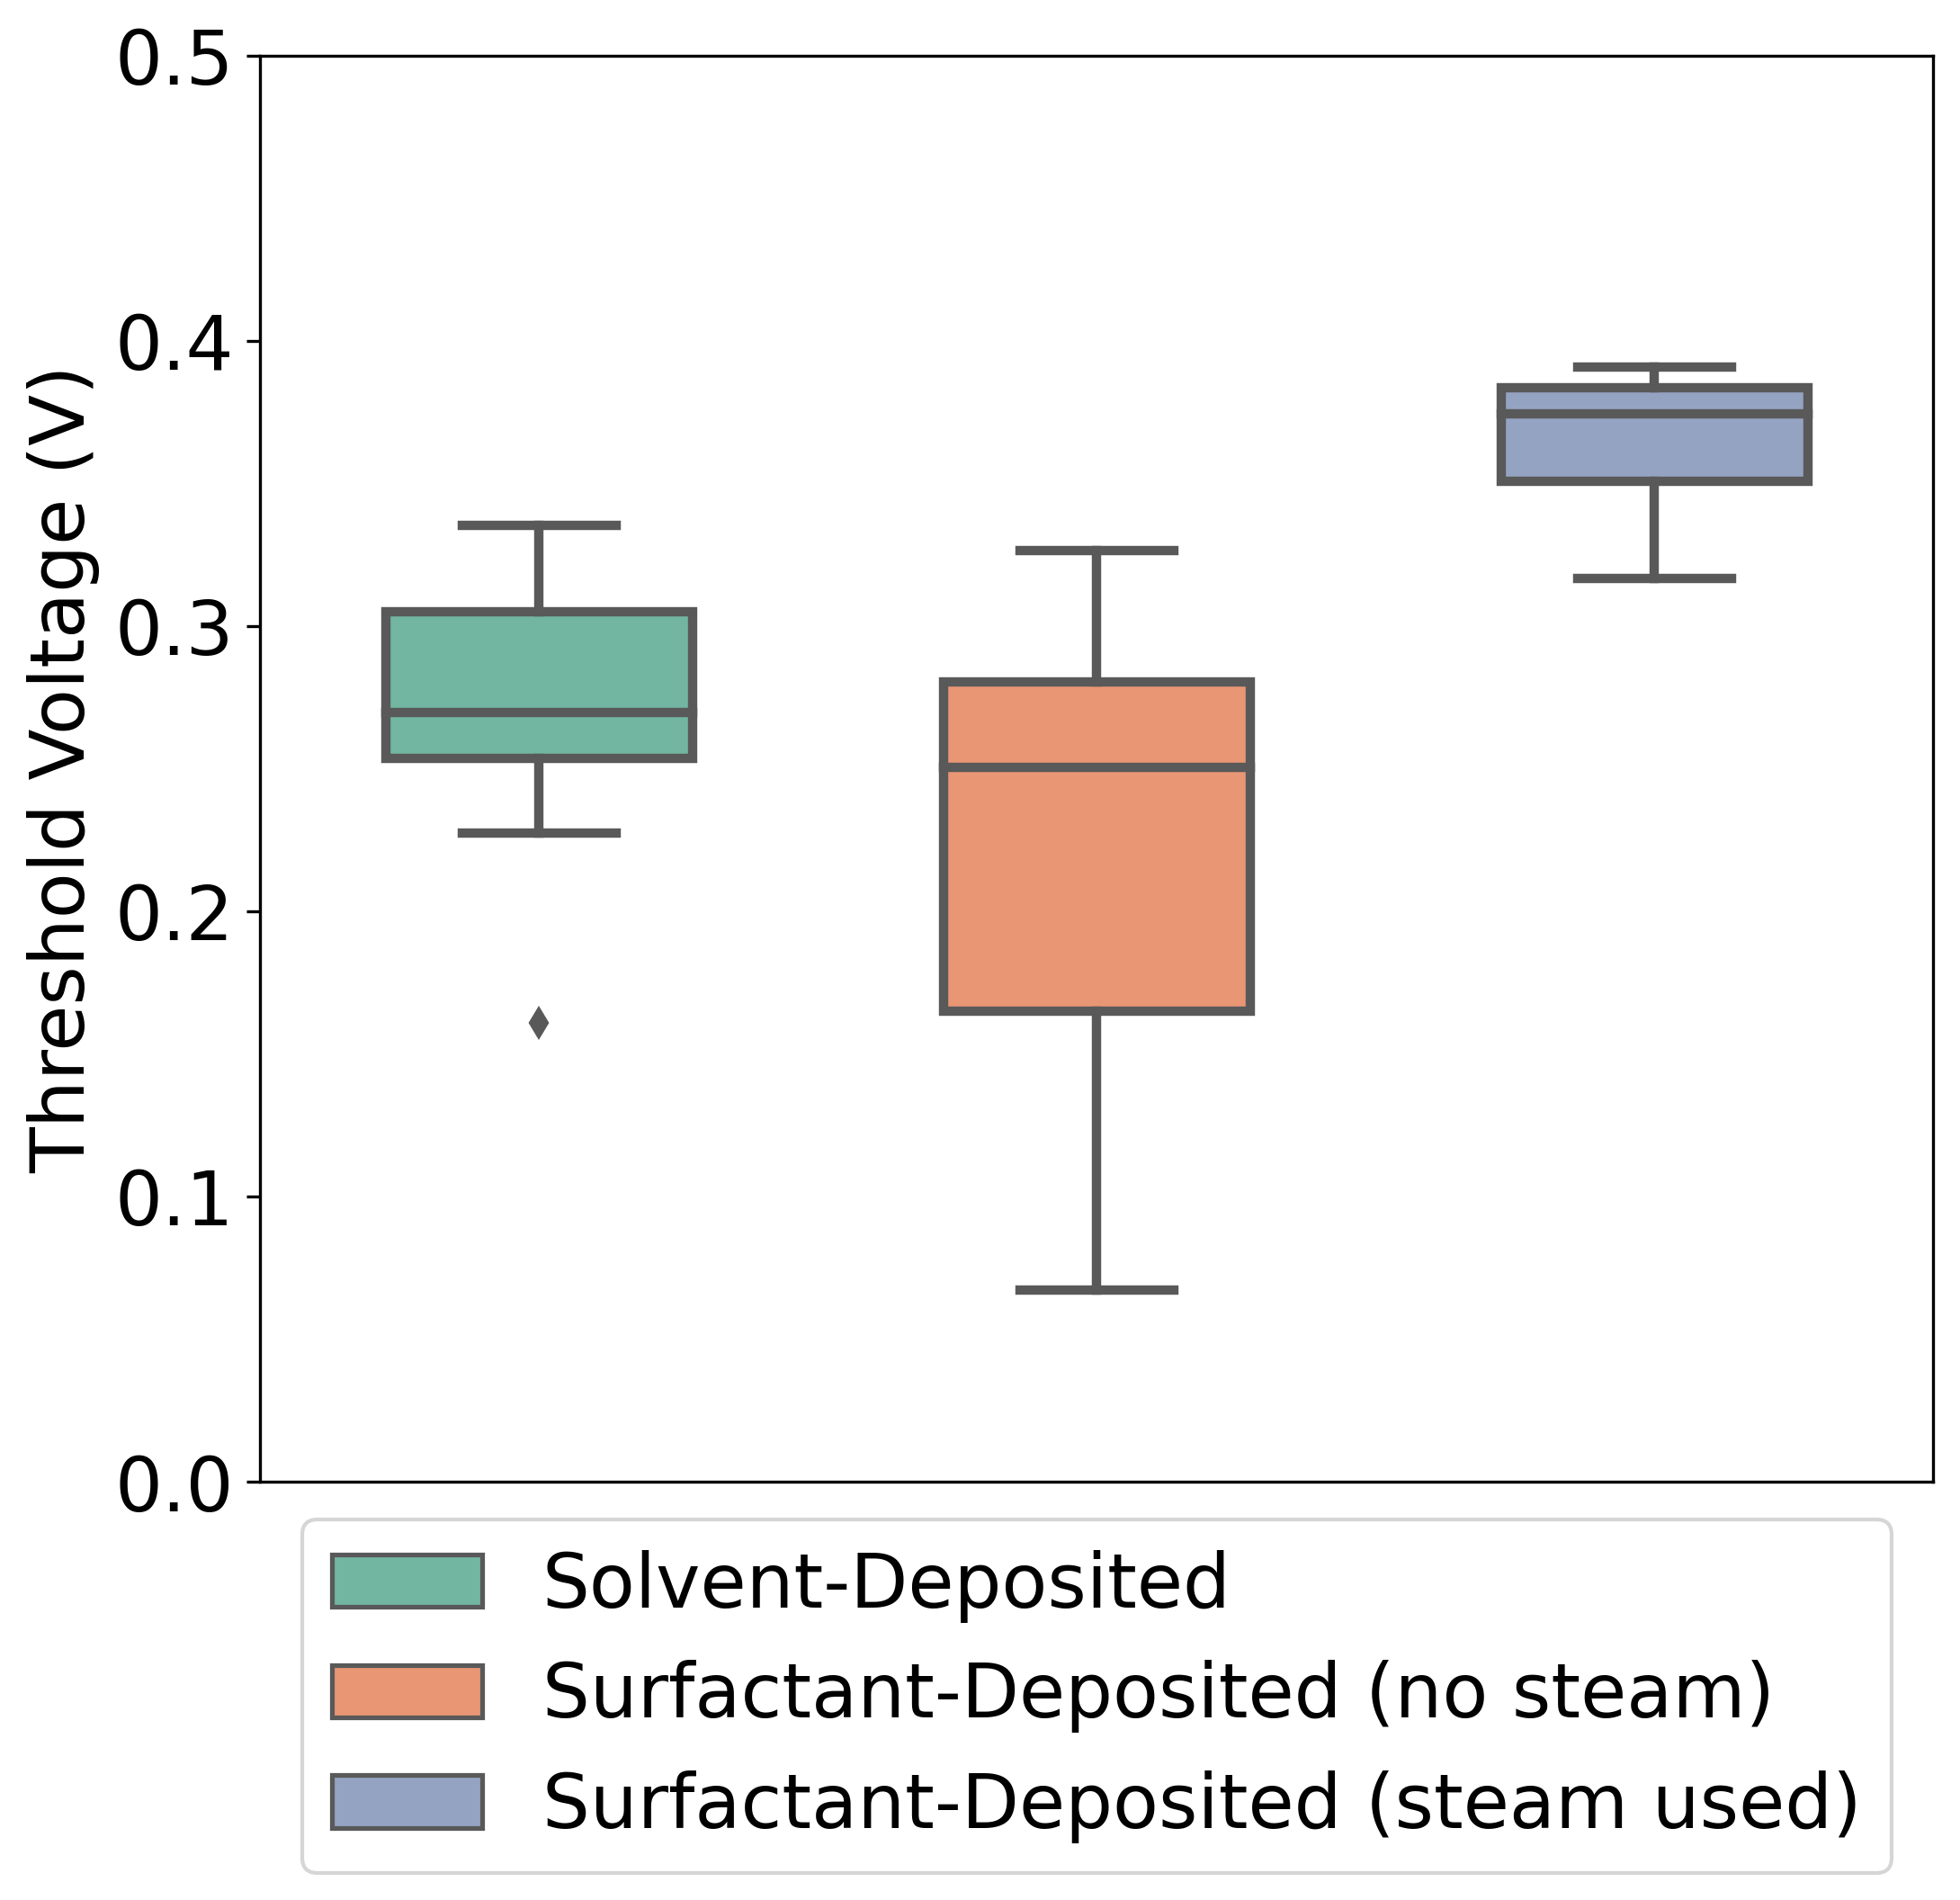
\includegraphics{figures/ch6/threshold_V.png}

}

}

\subcaption{\label{fig-threshold-voltage}}
\end{minipage}%
%
\begin{minipage}[t]{0.26\linewidth}

{\centering 

~

}

\end{minipage}%

\caption{\label{fig-sweep-parameters}These boxplots illustrate the
statistical distribution of (a) the on-off ratio, (b) the subthreshold
slope, and (c) the threshold voltage of AZ\(^\circledR\) 1518
encapsulated liquid-gated transistor channels corresponding to each type
of carbon nanotube film deposition. For each deposition type, electrical
characteristics were taken of 21 channels of at least three separate
devices. The boxes indicate the 25th and 75th percentile of the
distribution.}

\end{figure}

\hypertarget{liquid-gated-cntfets}{%
\subsubsection*{Liquid-Gated CNTFETs}\label{liquid-gated-cntfets}}
\addcontentsline{toc}{subsubsection}{Liquid-Gated CNTFETs}

The liquid-gated devices in Figure~\ref{fig-solvent-tx-lg},
Figure~\ref{fig-surf-tx-lg} and Figure~\ref{fig-steam-tx-lg} each
exhibited ambipolar characteristics, commonly observed in liquid-gated
carbon nanotube network FETs
\autocite{Kauffman2008,Heller2009,JongYu2009,Derenskyi2014,Murugathas2018,Albarghouthi2022}.
When devices were appropriately configured, leakage current (shown by
the dashed traces) did not exceed \(\sim 1 \times 10^{-7}\) V across the
forward and reverse sweep. The devices shown which used steam-deposited
carbon nanotube films showed the least hysteresis.
Section~\ref{sec-pristine-AFM} demonstrates that the mean diameter of
the bundles in these films is about 0.9 nm less than the mean bundles in
films deposited without steam present, and 5.5 nm less than those in
films deposited in solvent. Hysteresis is known to scale roughly
linearly with bundle diameter, due to trapped charge increasing as
bundle density of states is increased \autocite{Pop2009}.
Steam-deposited devices also showed significantly less
channel-to-channel variation in electrical characteristics more
generally. Channel 1 in Figure~\ref{fig-solvent-tx-lg} has a much higher
off-current than the other channels of the same device, which appears to
be due to a uncommonly high proportion of metallic carbon nanotubes
present in the network conduction pathways of this channel
\autocite{Rouhi2011,Zaumseil2015}.

A summary of key parameters of pristine liquid-gated devices is shown in
Figure~\ref{fig-sweep-parameters}. The full dataset consists of three
sets of 21 liquid-gated transfer characteristics of working channels,
with each set corresponding to the use of a particular method of carbon
nanotube network deposition in the device fabrication. Measurements from
at least three devices are included in each set. Each entry in the
summary corresponds to the average of the specific parameter in the
forward and reverse sweep direction. When steam was used for surfactant
deposition of films, the resulting devices showed highly consistent
channel-to-channel electrical properties. Since the carbon nanotube
films on these devices are relatively dense, as seen in
Figure~\ref{fig-steaming-network}, the network should be well above the
percolation threshold. As many carbon nanotube pathways connect across
the channel in parallel, small variations in the network morphology have
less of an impact on the overall channel behaviour
\autocite{Murugathas2018}. Figure~\ref{fig-cnt-histogram} and
Table~\ref{tbl-histogram-parameters} indicate that the range of bundle
sizes is relatively low in the steam-deposited films used in these
devices, meaning the electrical behaviour of dominant conduction
pathways is more spatially consistent. The repeatable subthreshold
regime behaviour between channels seen for steam-deposited devices is a
desirable attribute for reliable real-time multiplexed biosensing
\autocite{Kauffman2008,Heller2009,Gao2010}.

Channels from surfactant-deposited film devices usually showed a larger
on-off ratio and subthreshold slope than those from solvent-deposited
devices. Decreasing the ratio of gate-sensitive semiconducting carbon
nanotubes to metallic nanotubes tends to decrease the on-off ratio
\autocite{LeMieux2008,Rouhi2011,Zaumseil2015,Murugathas2018}.
Section~\ref{sec-pristine-raman} seems to indicate there are more
metallic nanotubes present in the surfactant-deposited films than in the
solvent-deposited films. However, percolating conduction pathways
dominate device behaviour and nanotube pathways across the channel with
a lower degree of bundling are less likely to contain metallic tubes
\autocite{Murugathas2018}. Therefore, the larger on-off ratio for
surfactant-deposited film devices is likely a result of their reduced
nanotube bundle size and reduced bundle size variation relative to other
films, as discussed in Section~\ref{sec-pristine-morphology}. The larger
subthreshold slope is likely due to increased mobility from a denser
nanotube network in surfactant-deposited films \autocite{Rouhi2011}, as
seen in Figure~\ref{fig-steaming-network}. A larger on-off ratio and
subthreshold slope results in a larger change in conductance in response
to changes in the transfer characteristic curve. Therefore, the larger
on-off ratio and subthreshold slope of steam-deposited devices is
desirable for improved sensor performance
\autocite{Kauffman2008,Heller2009,Gao2010}.

All channels characterised had a positive threshold voltage
(\(V_{th}\)). The threshold voltage was largest and most consistent for
steam-assisted surfactant-deposited films. The relatively high values of
\(V_{th}\) which correspond to channel measurements from steam-assisted
surfactant-deposited devices indicates increased \(p\)-doping of the
network relative to networks deposited via alternative processes
\autocite{Kang2005,Heller2008,Murugathas2018}. As seen from
Figure~\ref{fig-steamed-surfactant}-f and
Figure~\ref{fig-dg-peak-comparison}, the steam deposition process leads
to the presence of significant, persistent surfactant aggregates. It has
been previously established that residual surfactant can \(p\)-dope
carbon nanotubes, alongside enhancing \(p\)-doping from adsorped oxygen
and water \autocite{Kane2014,Nonoguchi2018,Christensen2022}. The
presence of residual surfactant may also explain the lowered
subthreshold slope, and therefore mobility, of the steam-deposited
devices relative to devices with films deposited in surfactant without
steam. The analysis by Kane \emph{et al.} shows that the thermal
annealling at 150°C used in this work to remove residual surfactant is
likely inadequate for this purpose. Oxidation of devices and vacuum
annealling at high temperatures (\textgreater{} 600°C) may be required
for effective desorption of the persistent surfactant
\autocite{Kane2014,Barnett2018}. Devices using films made using the
alternative two methods have the advantage of not requiring careful
treatment to remove surfactant.

\hypertarget{back-gated-cntfets}{%
\subsubsection*{Back-Gated CNTFETs}\label{back-gated-cntfets}}
\addcontentsline{toc}{subsubsection}{Back-Gated CNTFETs}

When characterising devices using the vapour delivery system chip
carrier, the setup arrangement meant all measurements were taken using a
backgate. Figure~\ref{fig-solvent-tx-bg}, Figure~\ref{fig-surf-tx-bg}
and Figure~\ref{fig-steam-tx-bg} show that backgated devices exhibit
\emph{p}-type transistor behaviour. Gate current leakage was negligible,
as shown by the dashed line staying close to zero across the sweep.
Significant hysteresis was observed. The hysteresis can be explained by
the presence of defects or charge traps within and on the surface of the
silicon dioxide and at interfaces between the silicon dioxide and carbon
nanotubes \autocite{Lee2007,Lee2012,Ha2014}. The hysteresis observed was
much greater than for the corresponding liquid-gated sweeps on the
right. The devices fabricated with a solvent-based deposition were
switched off at a lower voltage than the devices which used surfactant
during deposition.

\begin{figure}

\begin{minipage}[t]{0.47\linewidth}

{\centering 

\raisebox{-\height}{

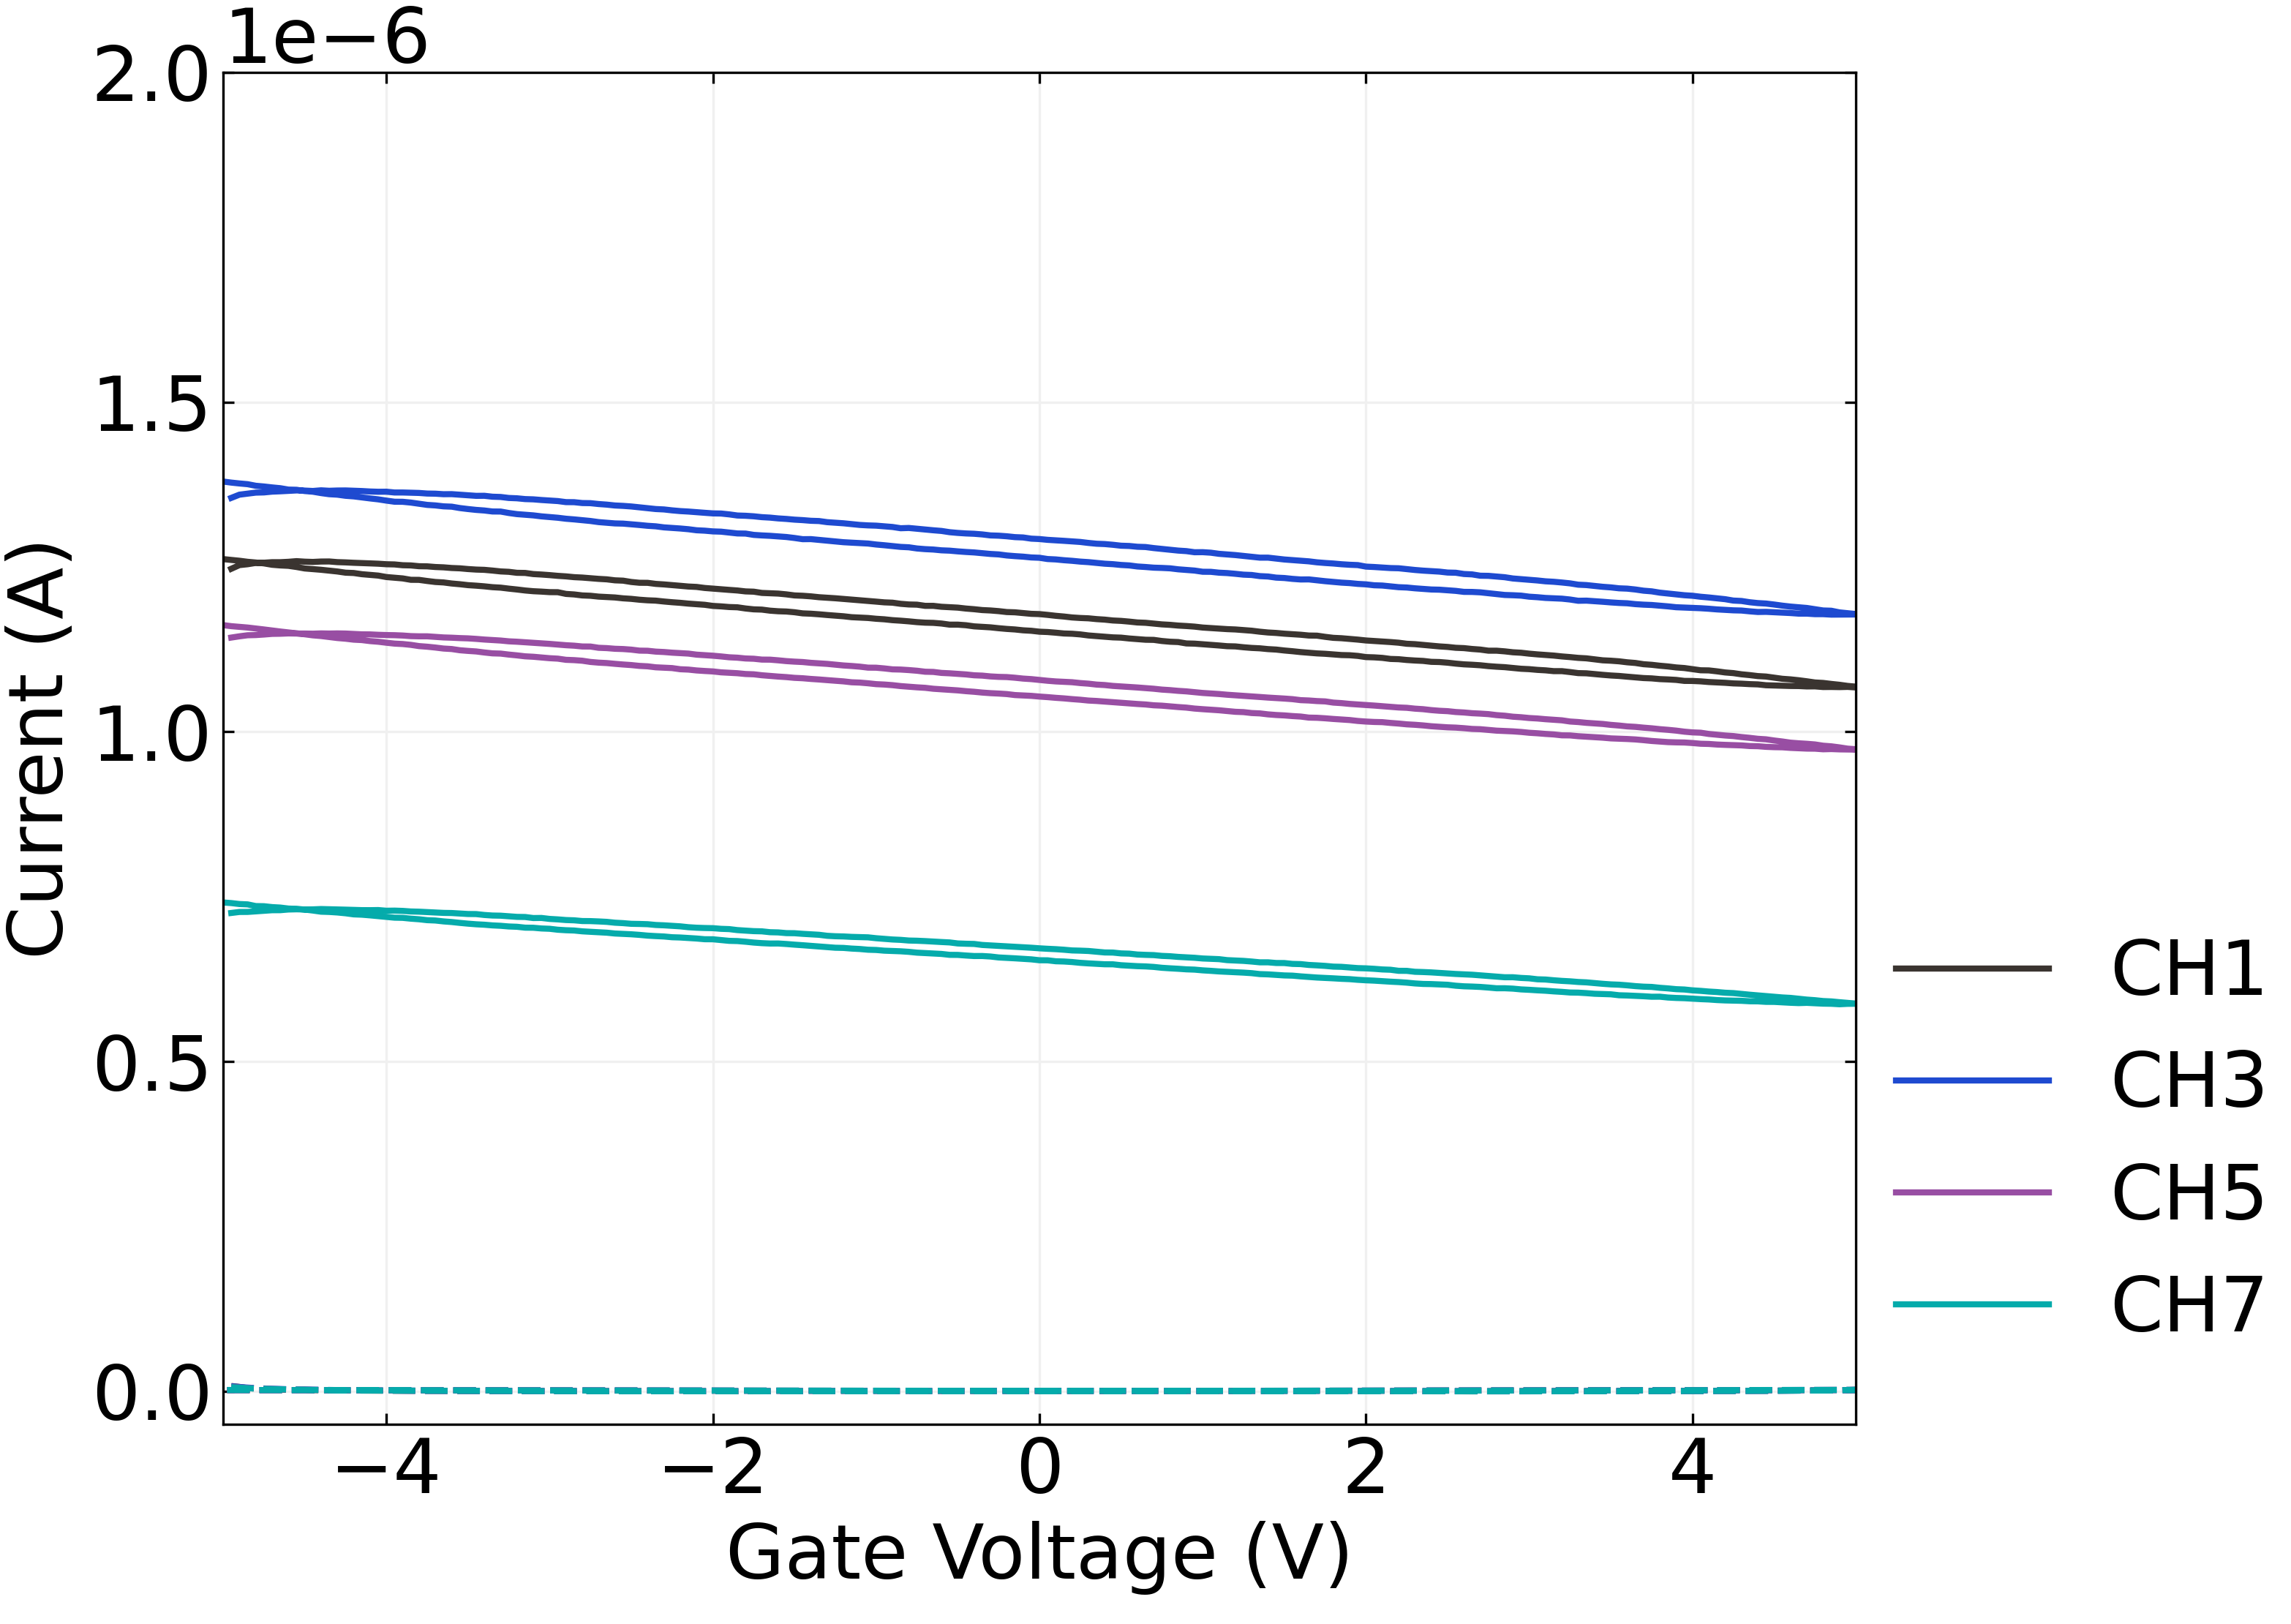
\includegraphics{figures/ch6/Q35C3_nobuffer.png}

}

}

\subcaption{\label{fig-no-buffer}}
\end{minipage}%
%
\begin{minipage}[t]{0.05\linewidth}

{\centering 

~

}

\end{minipage}%
%
\begin{minipage}[t]{0.47\linewidth}

{\centering 

\raisebox{-\height}{

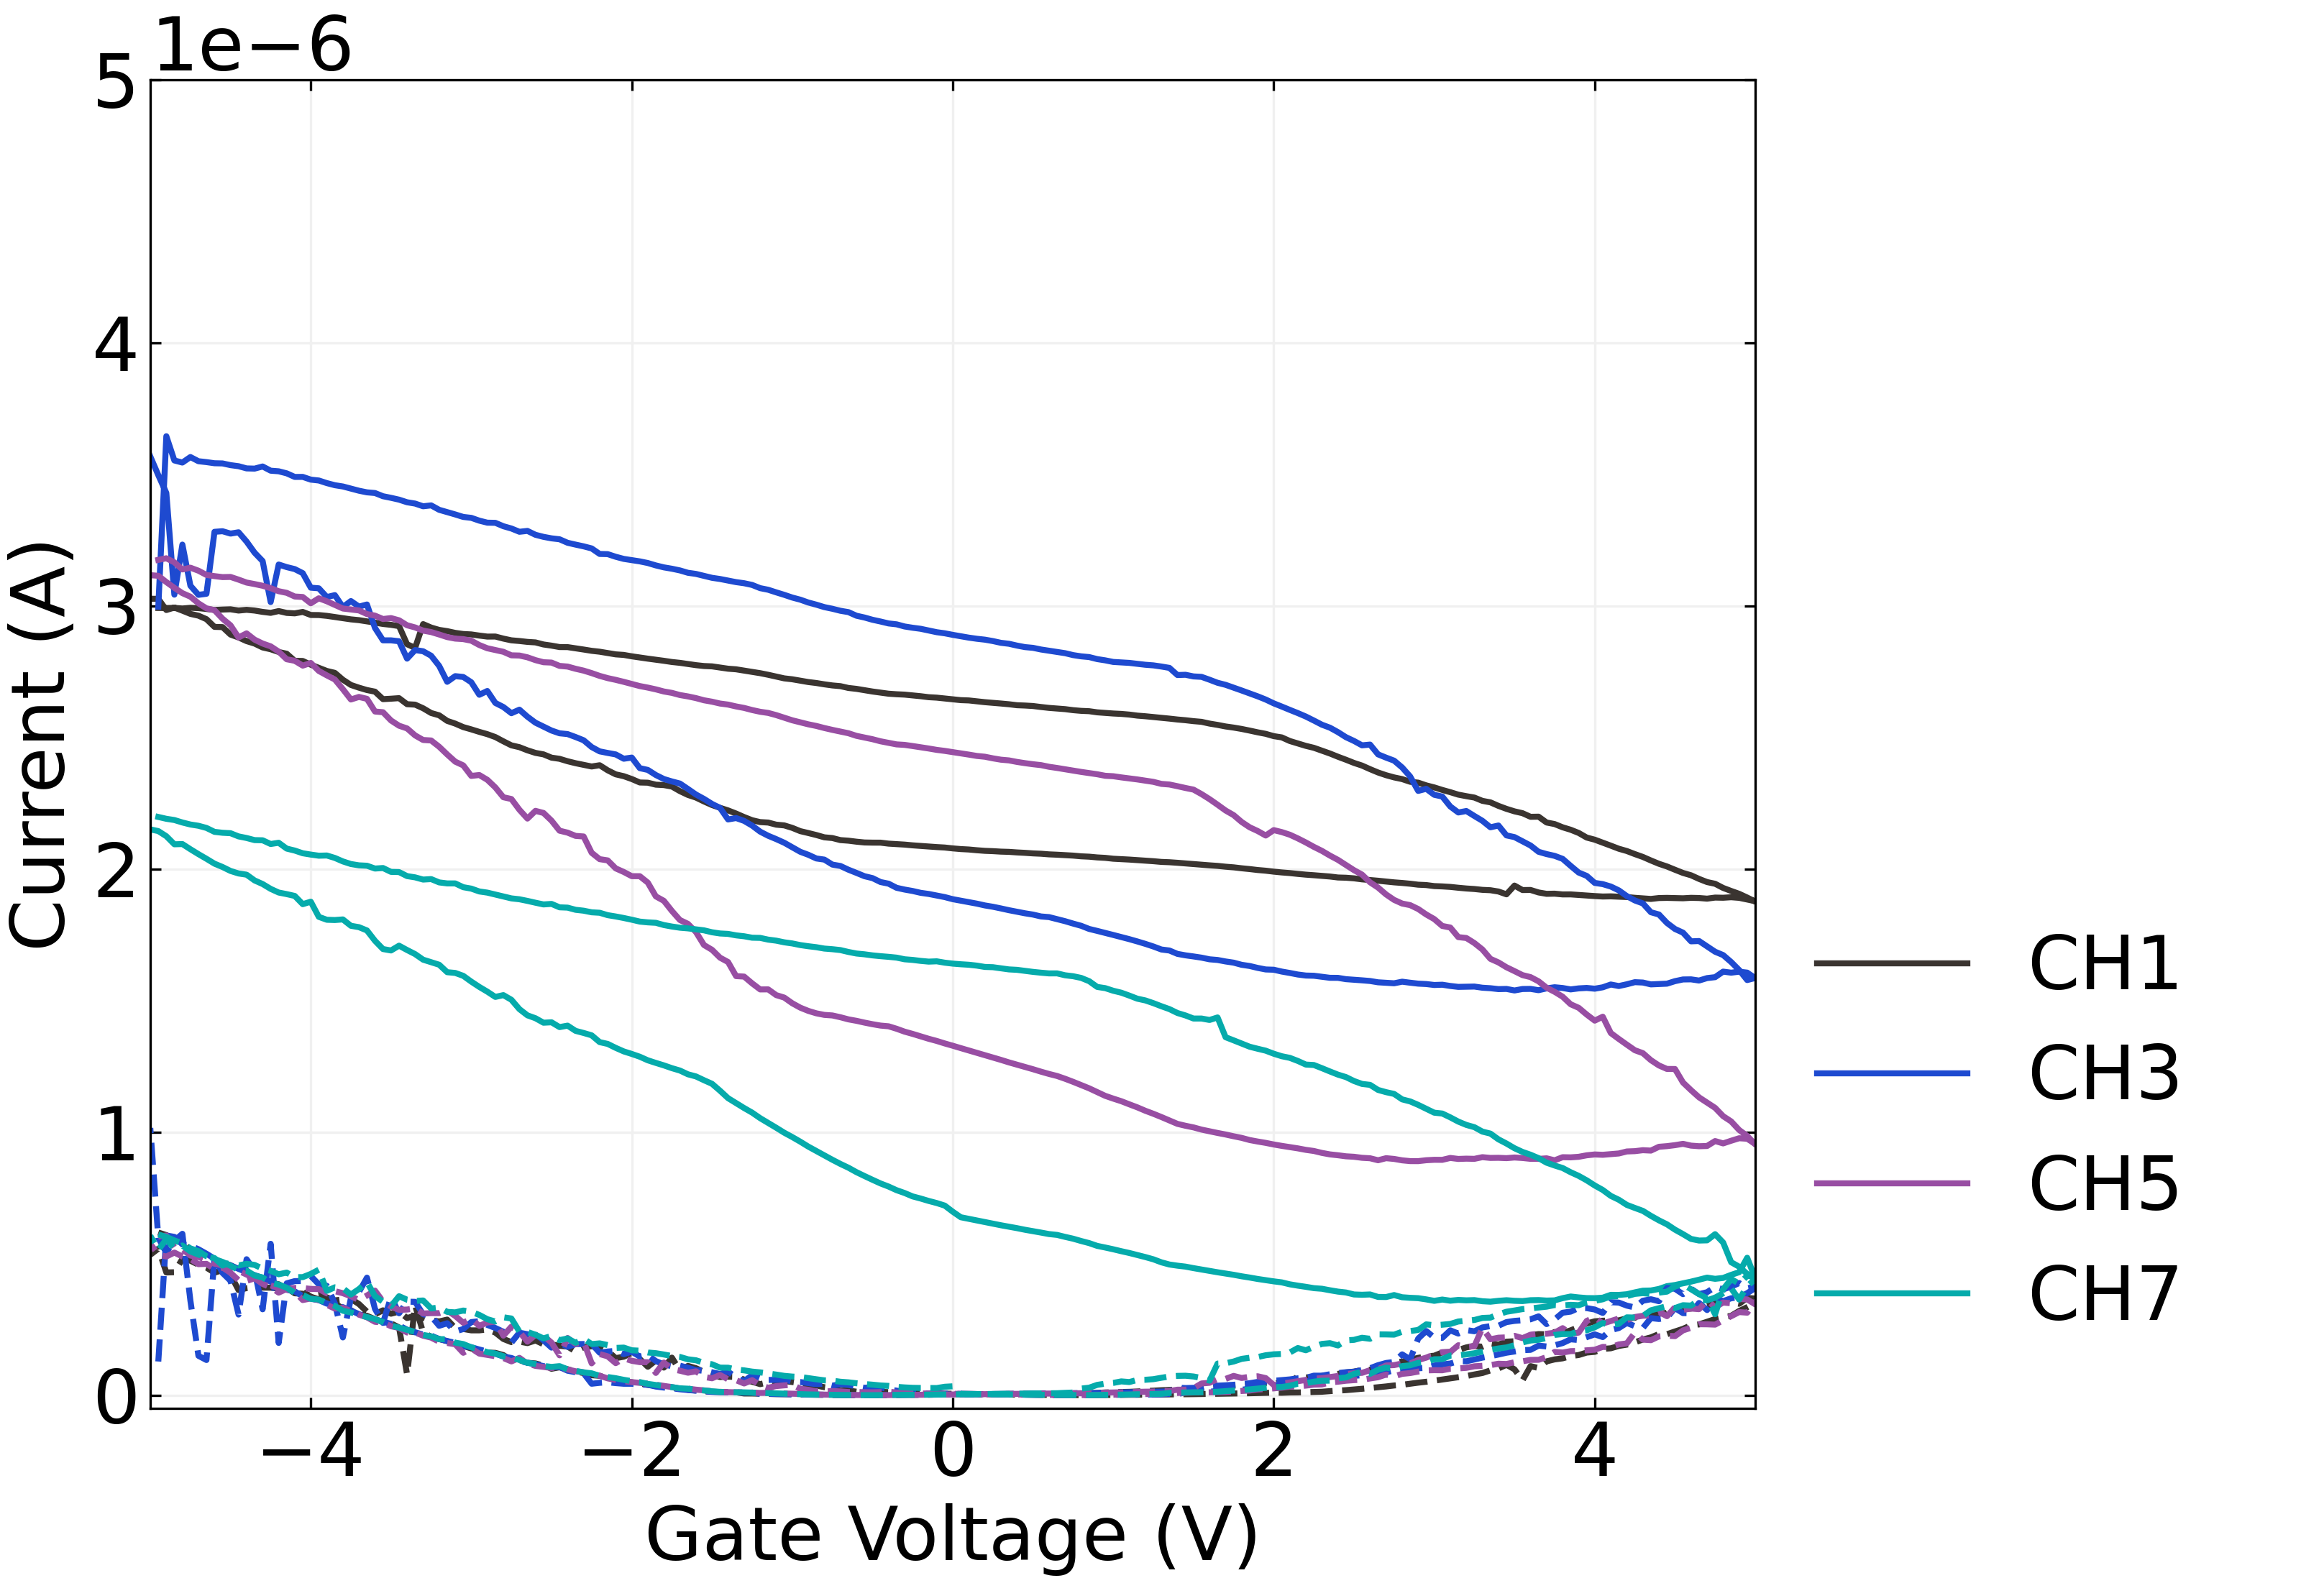
\includegraphics{figures/ch6/Q35C3_buffer.png}

}

}

\subcaption{\label{fig-50uL-buffer}}
\end{minipage}%

\caption{\label{fig-buffer-effect-on-backgate}Backgated transfer sweeps
were taken of an single unencapsulated device with a 300 nm SiO\(_2\)
layer and steam assisted surfactant-deposited carbon nanotube network
channels before and after being covered in \(50 \mu\)L 1XPBS
electrolyte.}

\end{figure}

Transfer measurements were taken to determine whether backgated
measurements could be taken of an unencapsulated device in the vapour
sensor chamber with 1XPBS covering the channels.
Figure~\ref{fig-buffer-effect-on-backgate} shows the behaviour of an
unencapsulated backgated device with a 300 nm SiO\(_2\) layer before and
after being covered by 50 \(\mu\)L of 1XPBS (phosphate buffered saline).
The on-off ratio and hysteresis of the channels increase significantly.
The presence of water increases hysteresis through introducing charge
traps at the silicon dioxide surface around the carbon nanotubes and at
the surface of the nanotubes themselves
\autocite{Kim2003,Lee2007,Franklin2012,Ha2014}. There is also a
significant increase in current leakage to the backgate for larger
applied voltages, despite the electrolyte having no visible physical
contact with the silicon backgate or copper plane. This leakage current
may simply be due to an increase in relative humidity around the device
due to the presence of water \autocite{Conseil2014}. As any variation in
threshold voltage due to hysteresis and significant leakage current are
undesirable for sensing procedures, this configuration was not used for
vapour sensing purposes.

\hypertarget{graphene-devices}{%
\subsection{Graphene Devices}\label{graphene-devices}}

\begin{figure}

\begin{minipage}[t]{0.47\linewidth}

{\centering 

\raisebox{-\height}{

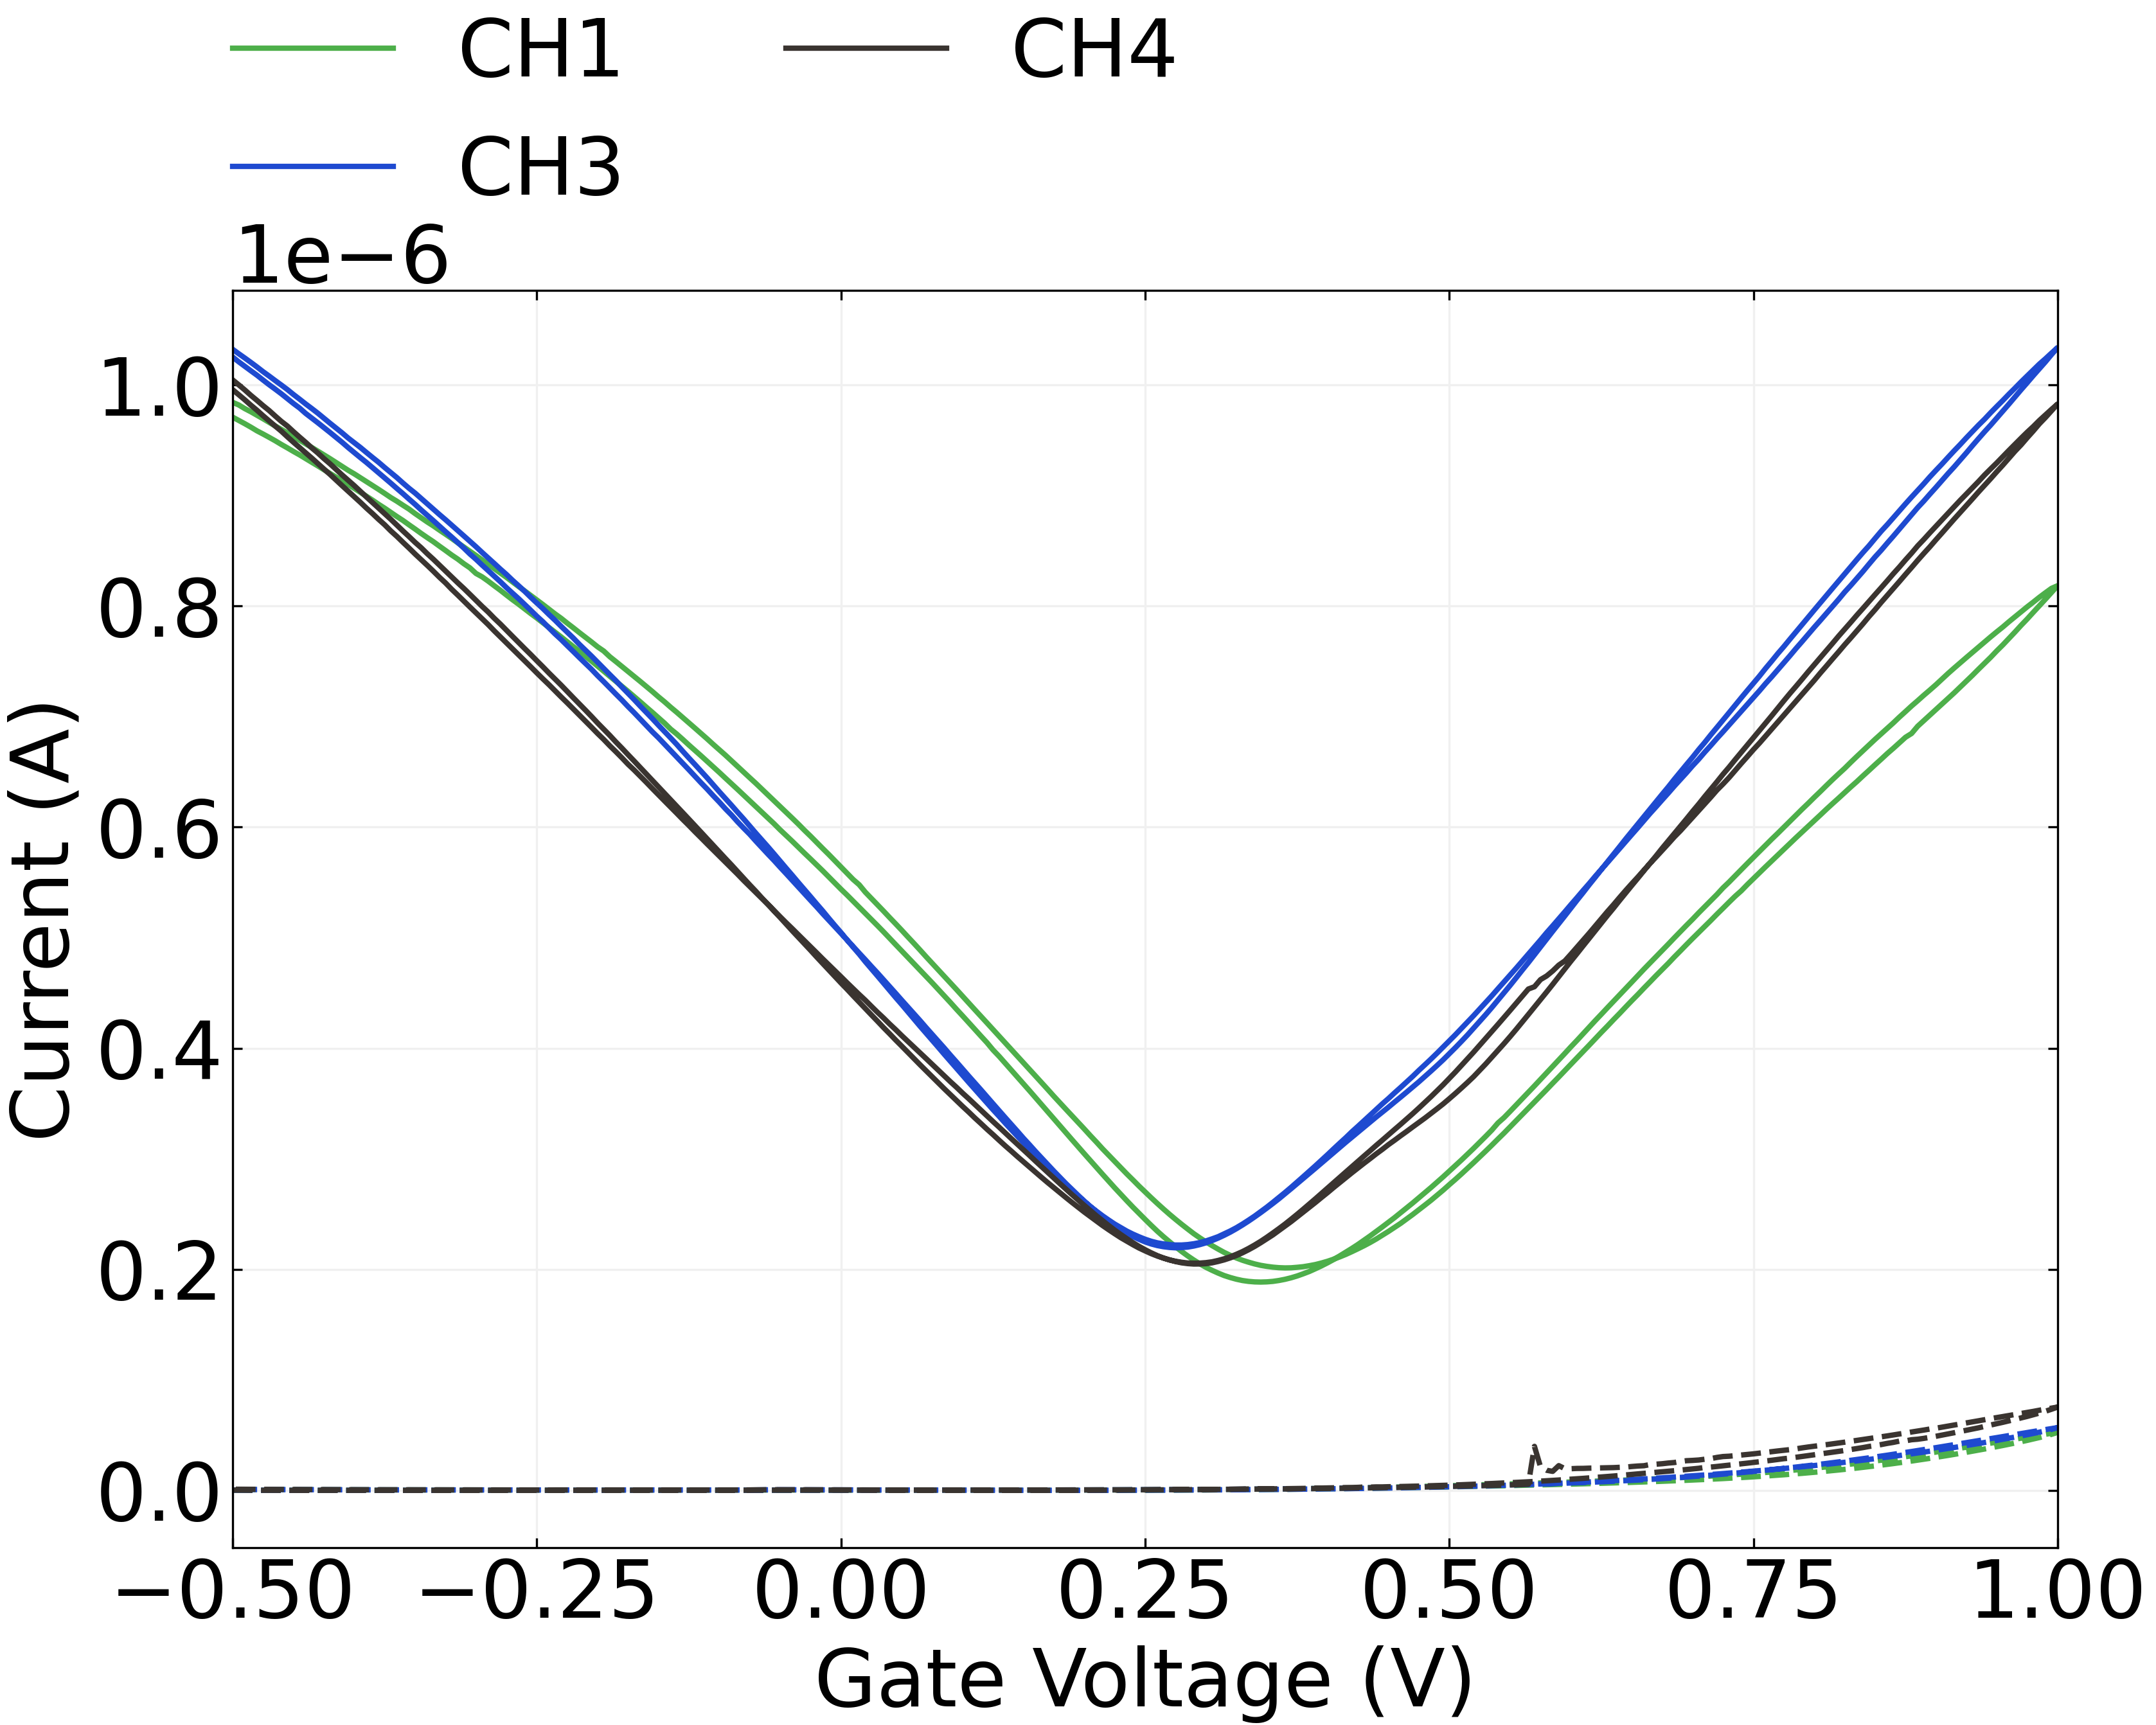
\includegraphics{figures/ch6/JG098_pristine_TXLG01_5mVstep_220920_norinse.png}

}

}

\subcaption{\label{fig-graphene-transfer-1}}
\end{minipage}%
%
\begin{minipage}[t]{0.05\linewidth}

{\centering 

~

}

\end{minipage}%
%
\begin{minipage}[t]{0.47\linewidth}

{\centering 

\raisebox{-\height}{

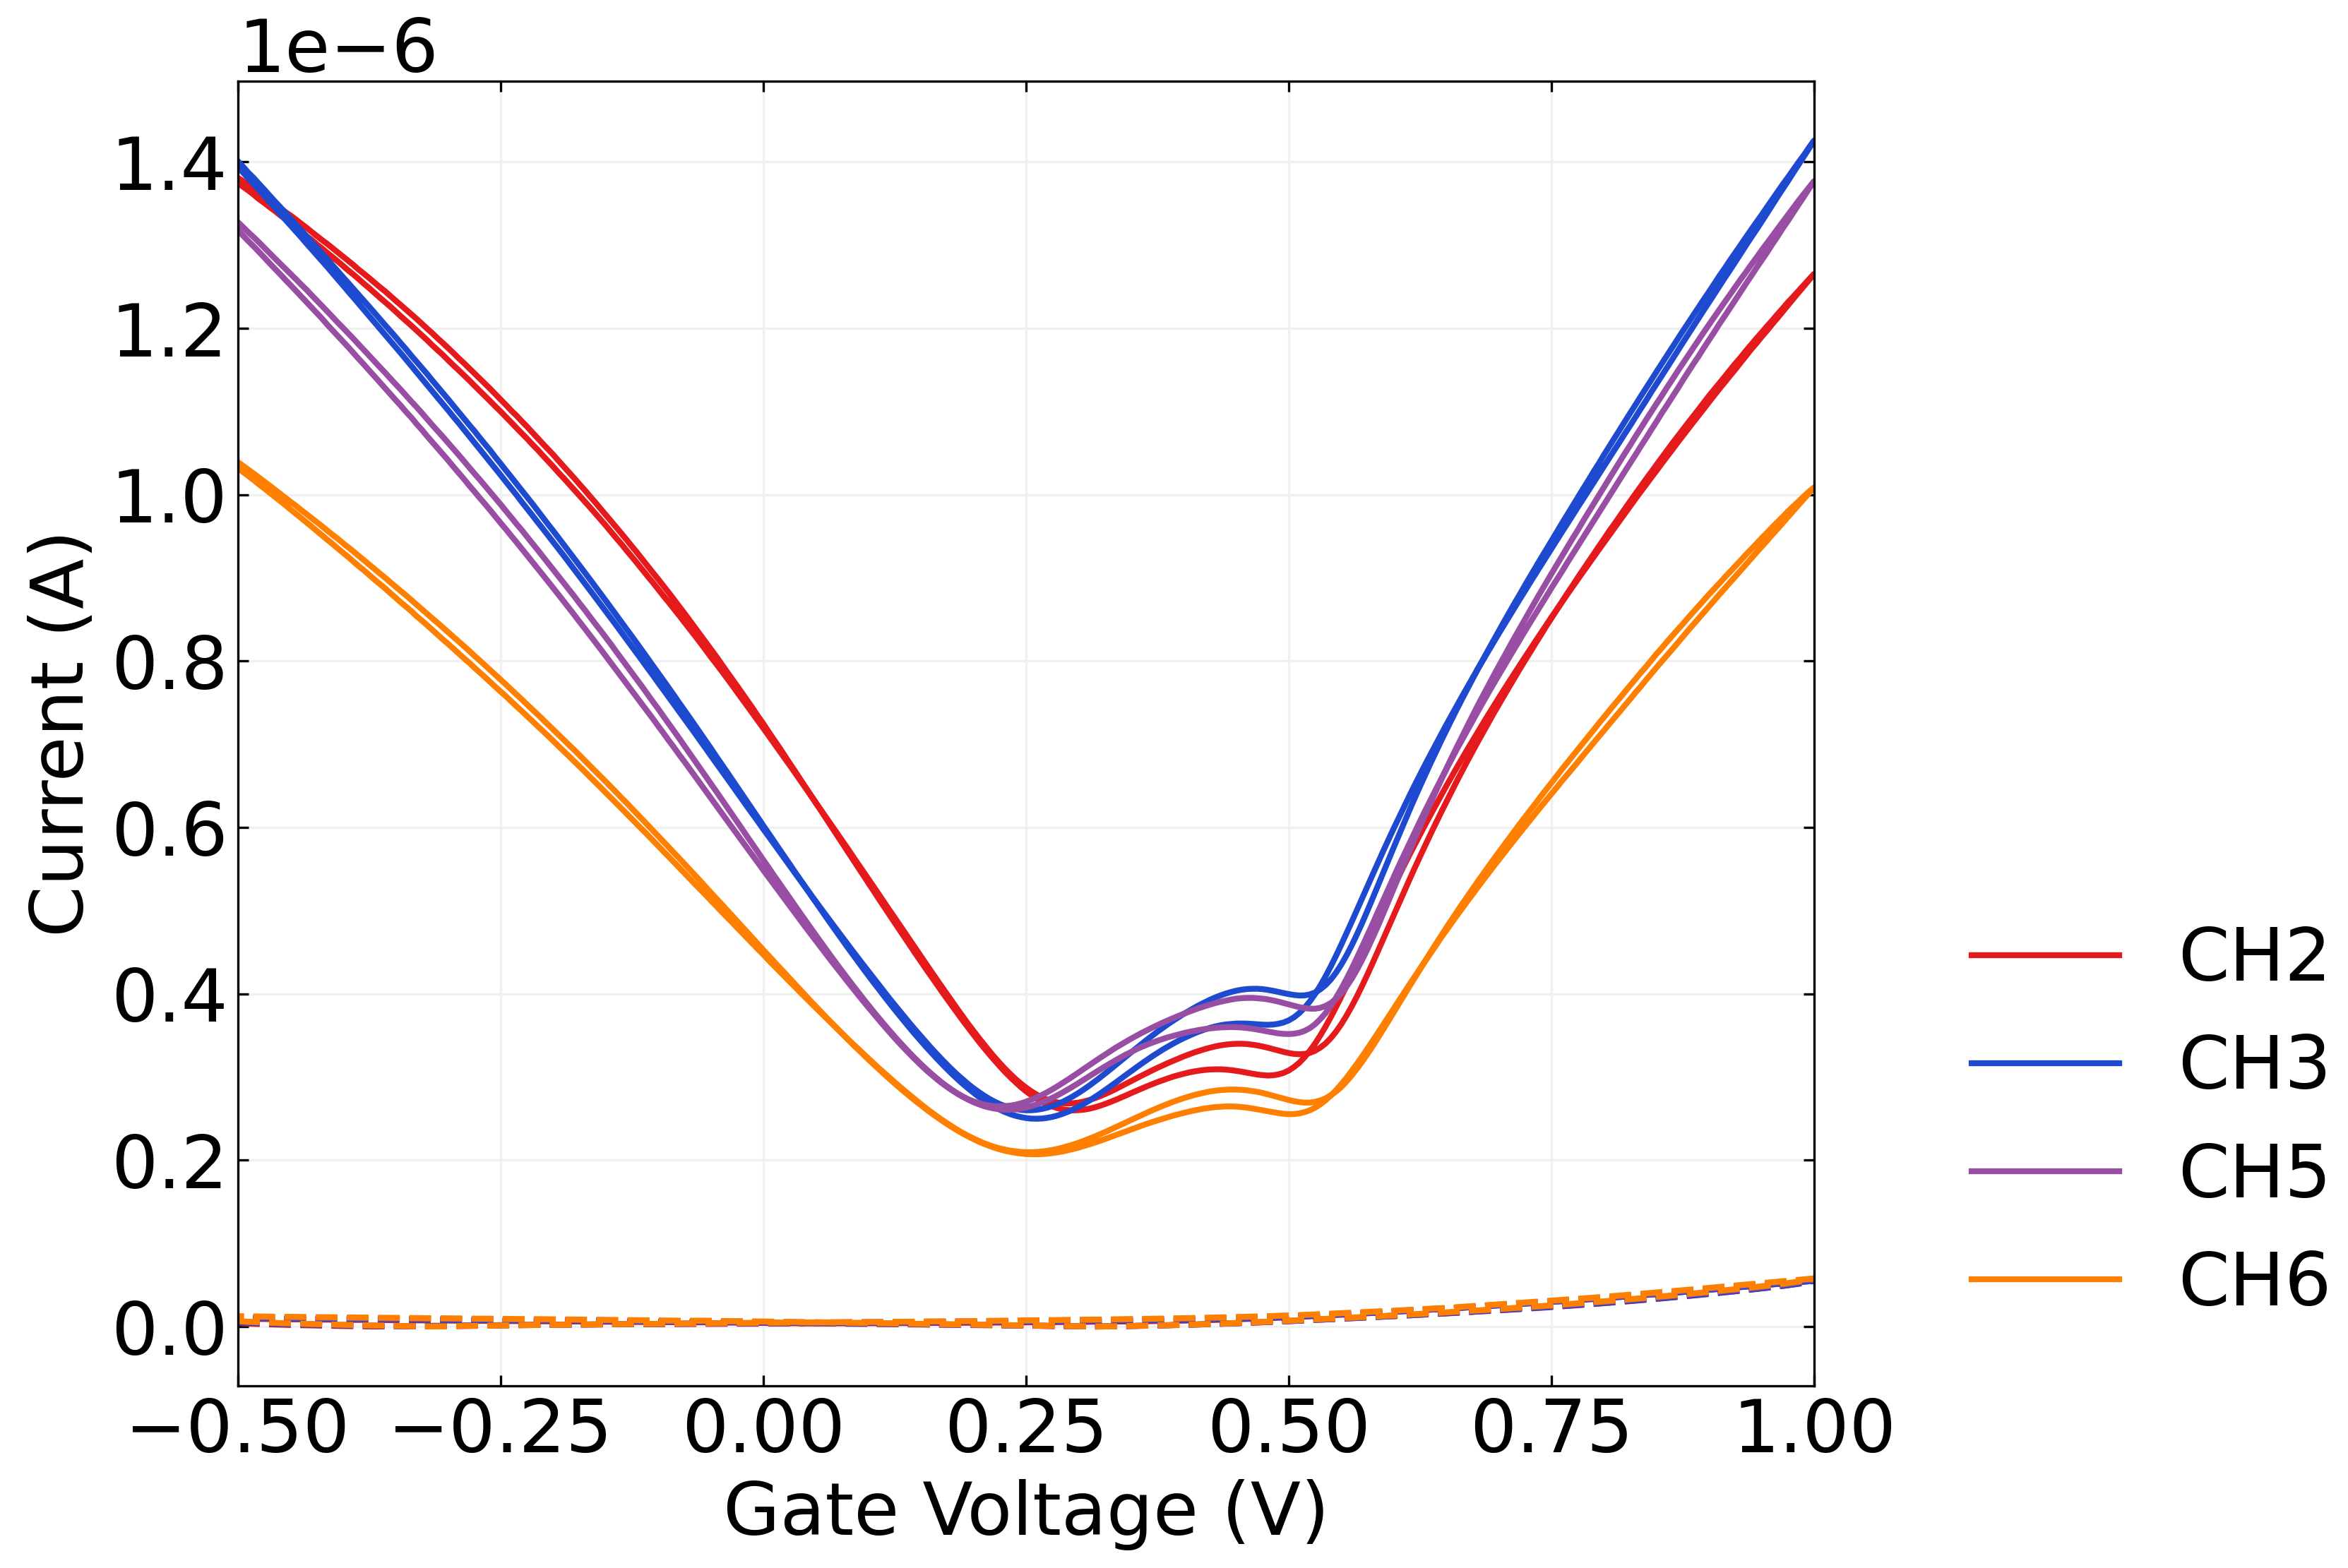
\includegraphics{figures/ch6/JGQ00D6_pristine_TXLG01_5mVstep_220914_norinse.png}

}

}

\subcaption{\label{fig-graphene-transfer-2}}
\end{minipage}%
\newline
\begin{minipage}[t]{0.47\linewidth}

{\centering 

\raisebox{-\height}{

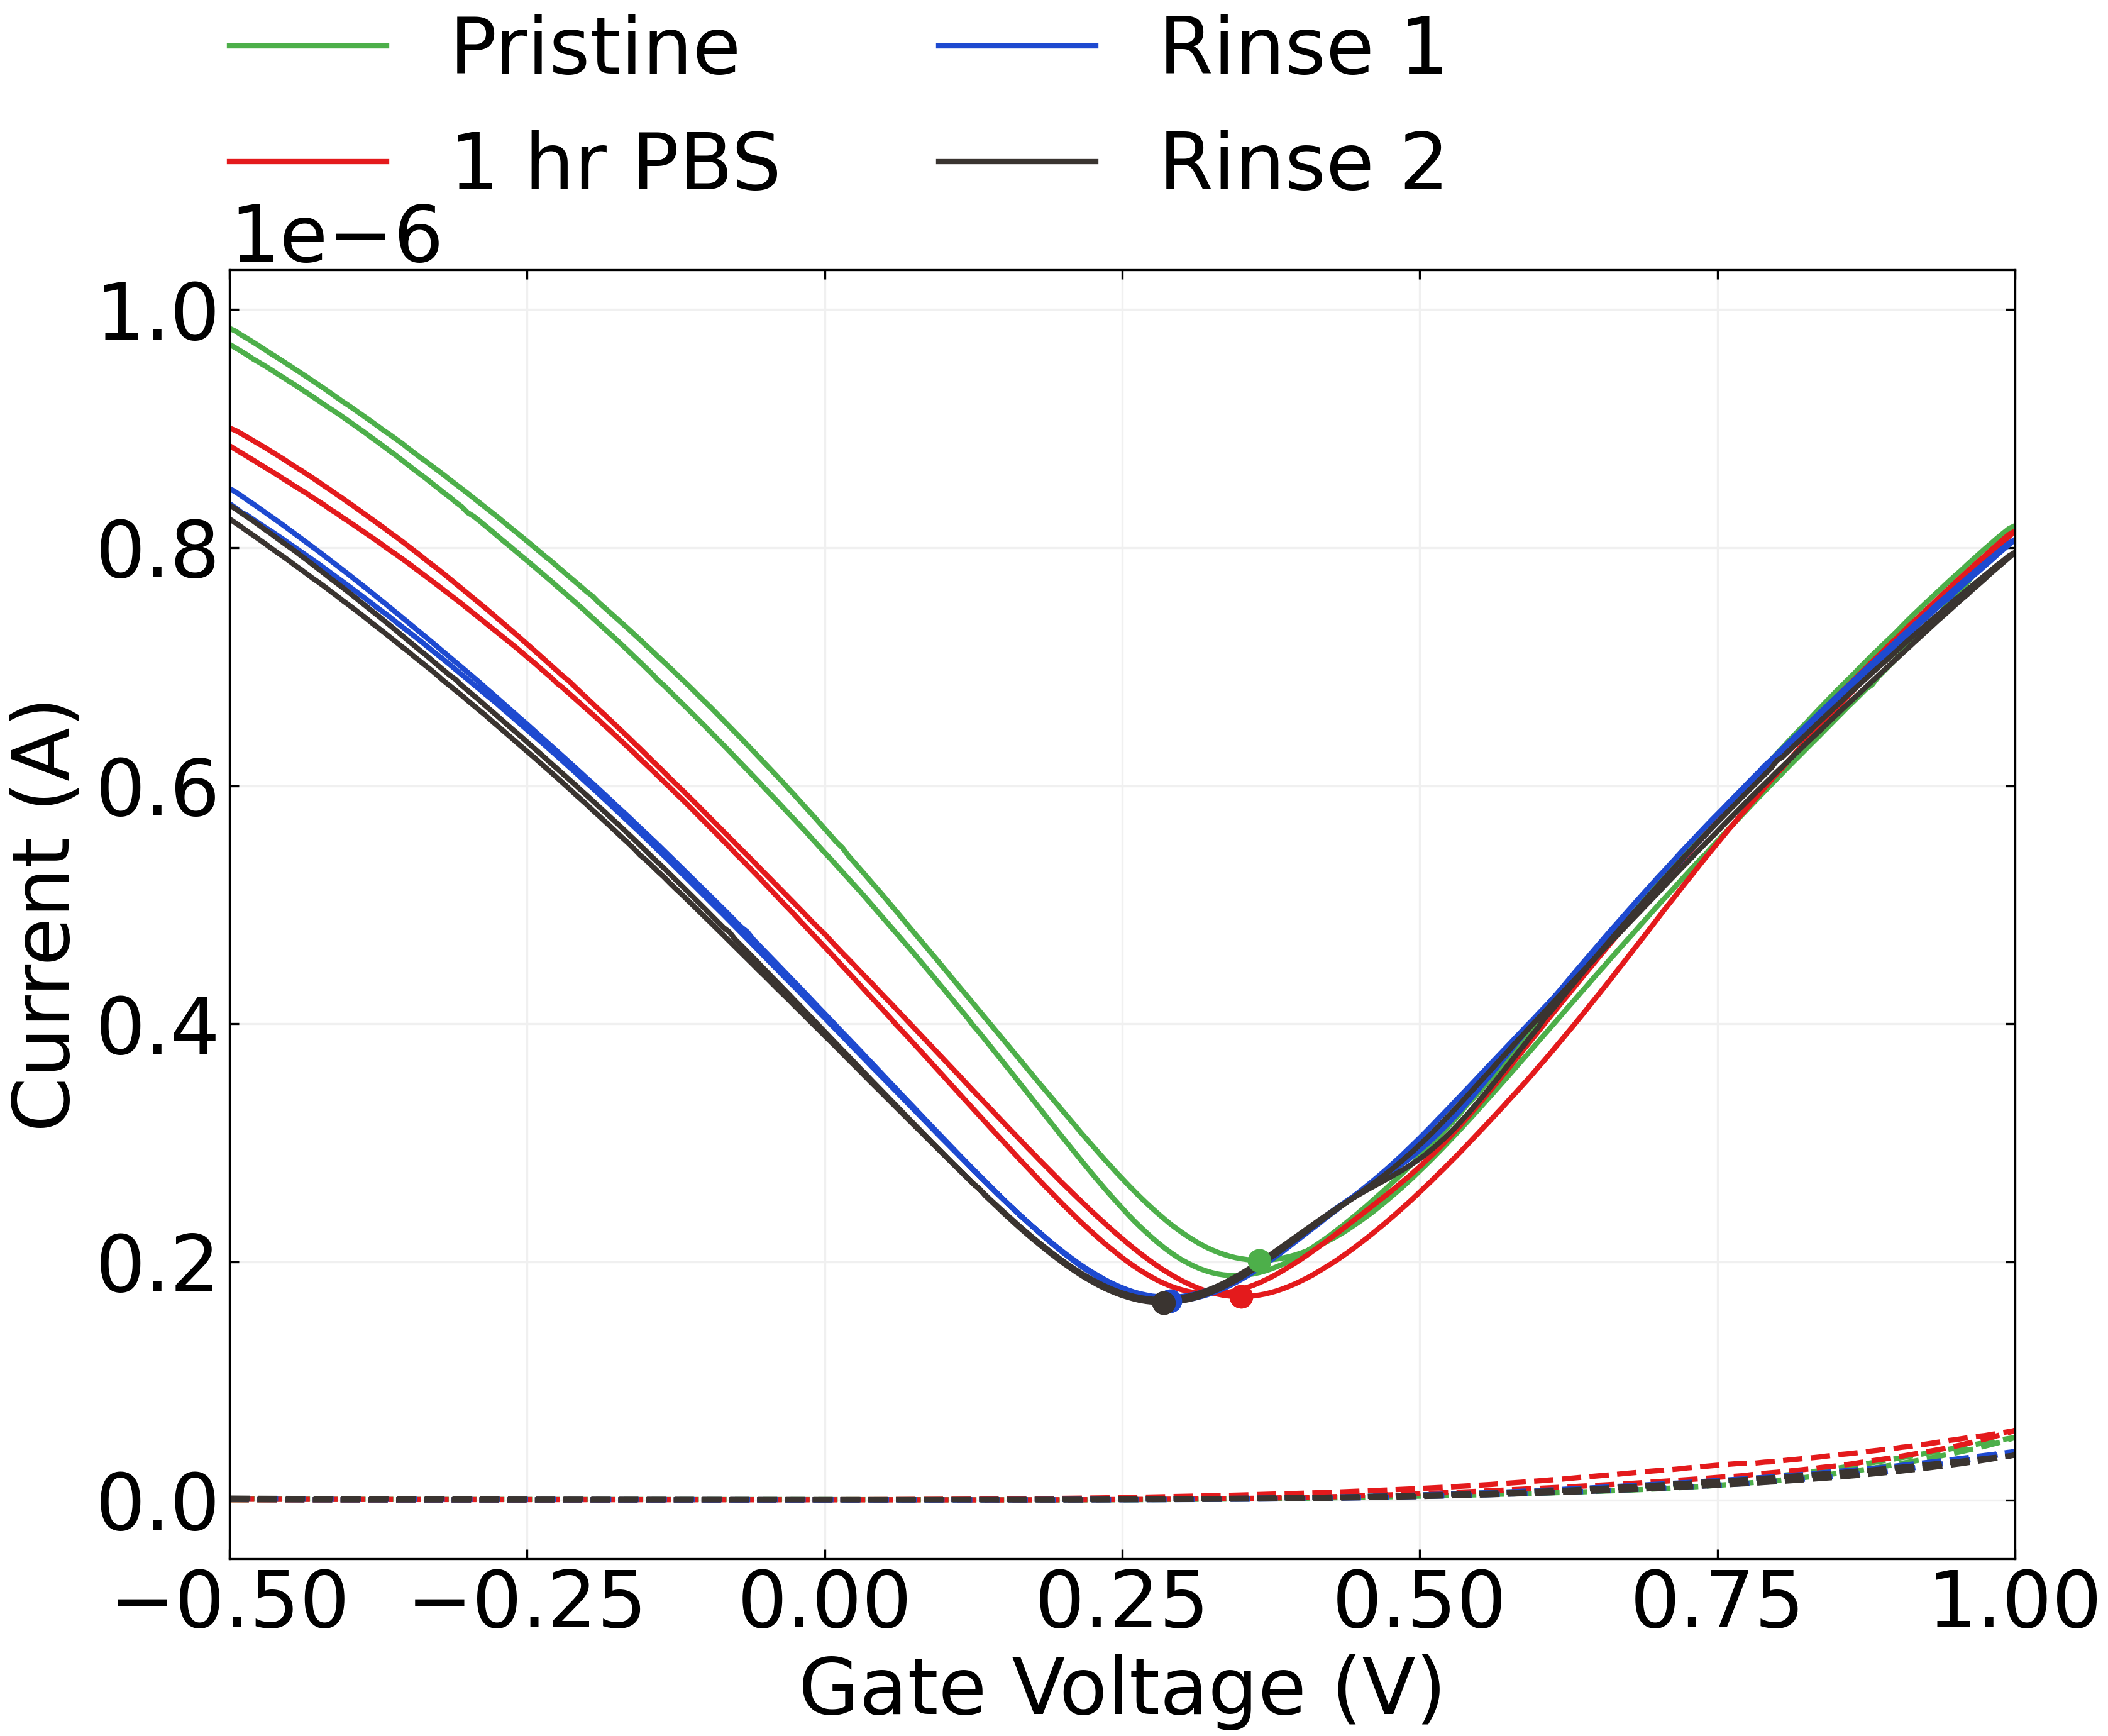
\includegraphics{figures/ch6/JG098_ch1_absolute_values_with_gate_current.png}

}

}

\subcaption{\label{fig-graphene-transfer-comparison-1}}
\end{minipage}%
%
\begin{minipage}[t]{0.05\linewidth}

{\centering 

~

}

\end{minipage}%
%
\begin{minipage}[t]{0.47\linewidth}

{\centering 

\raisebox{-\height}{

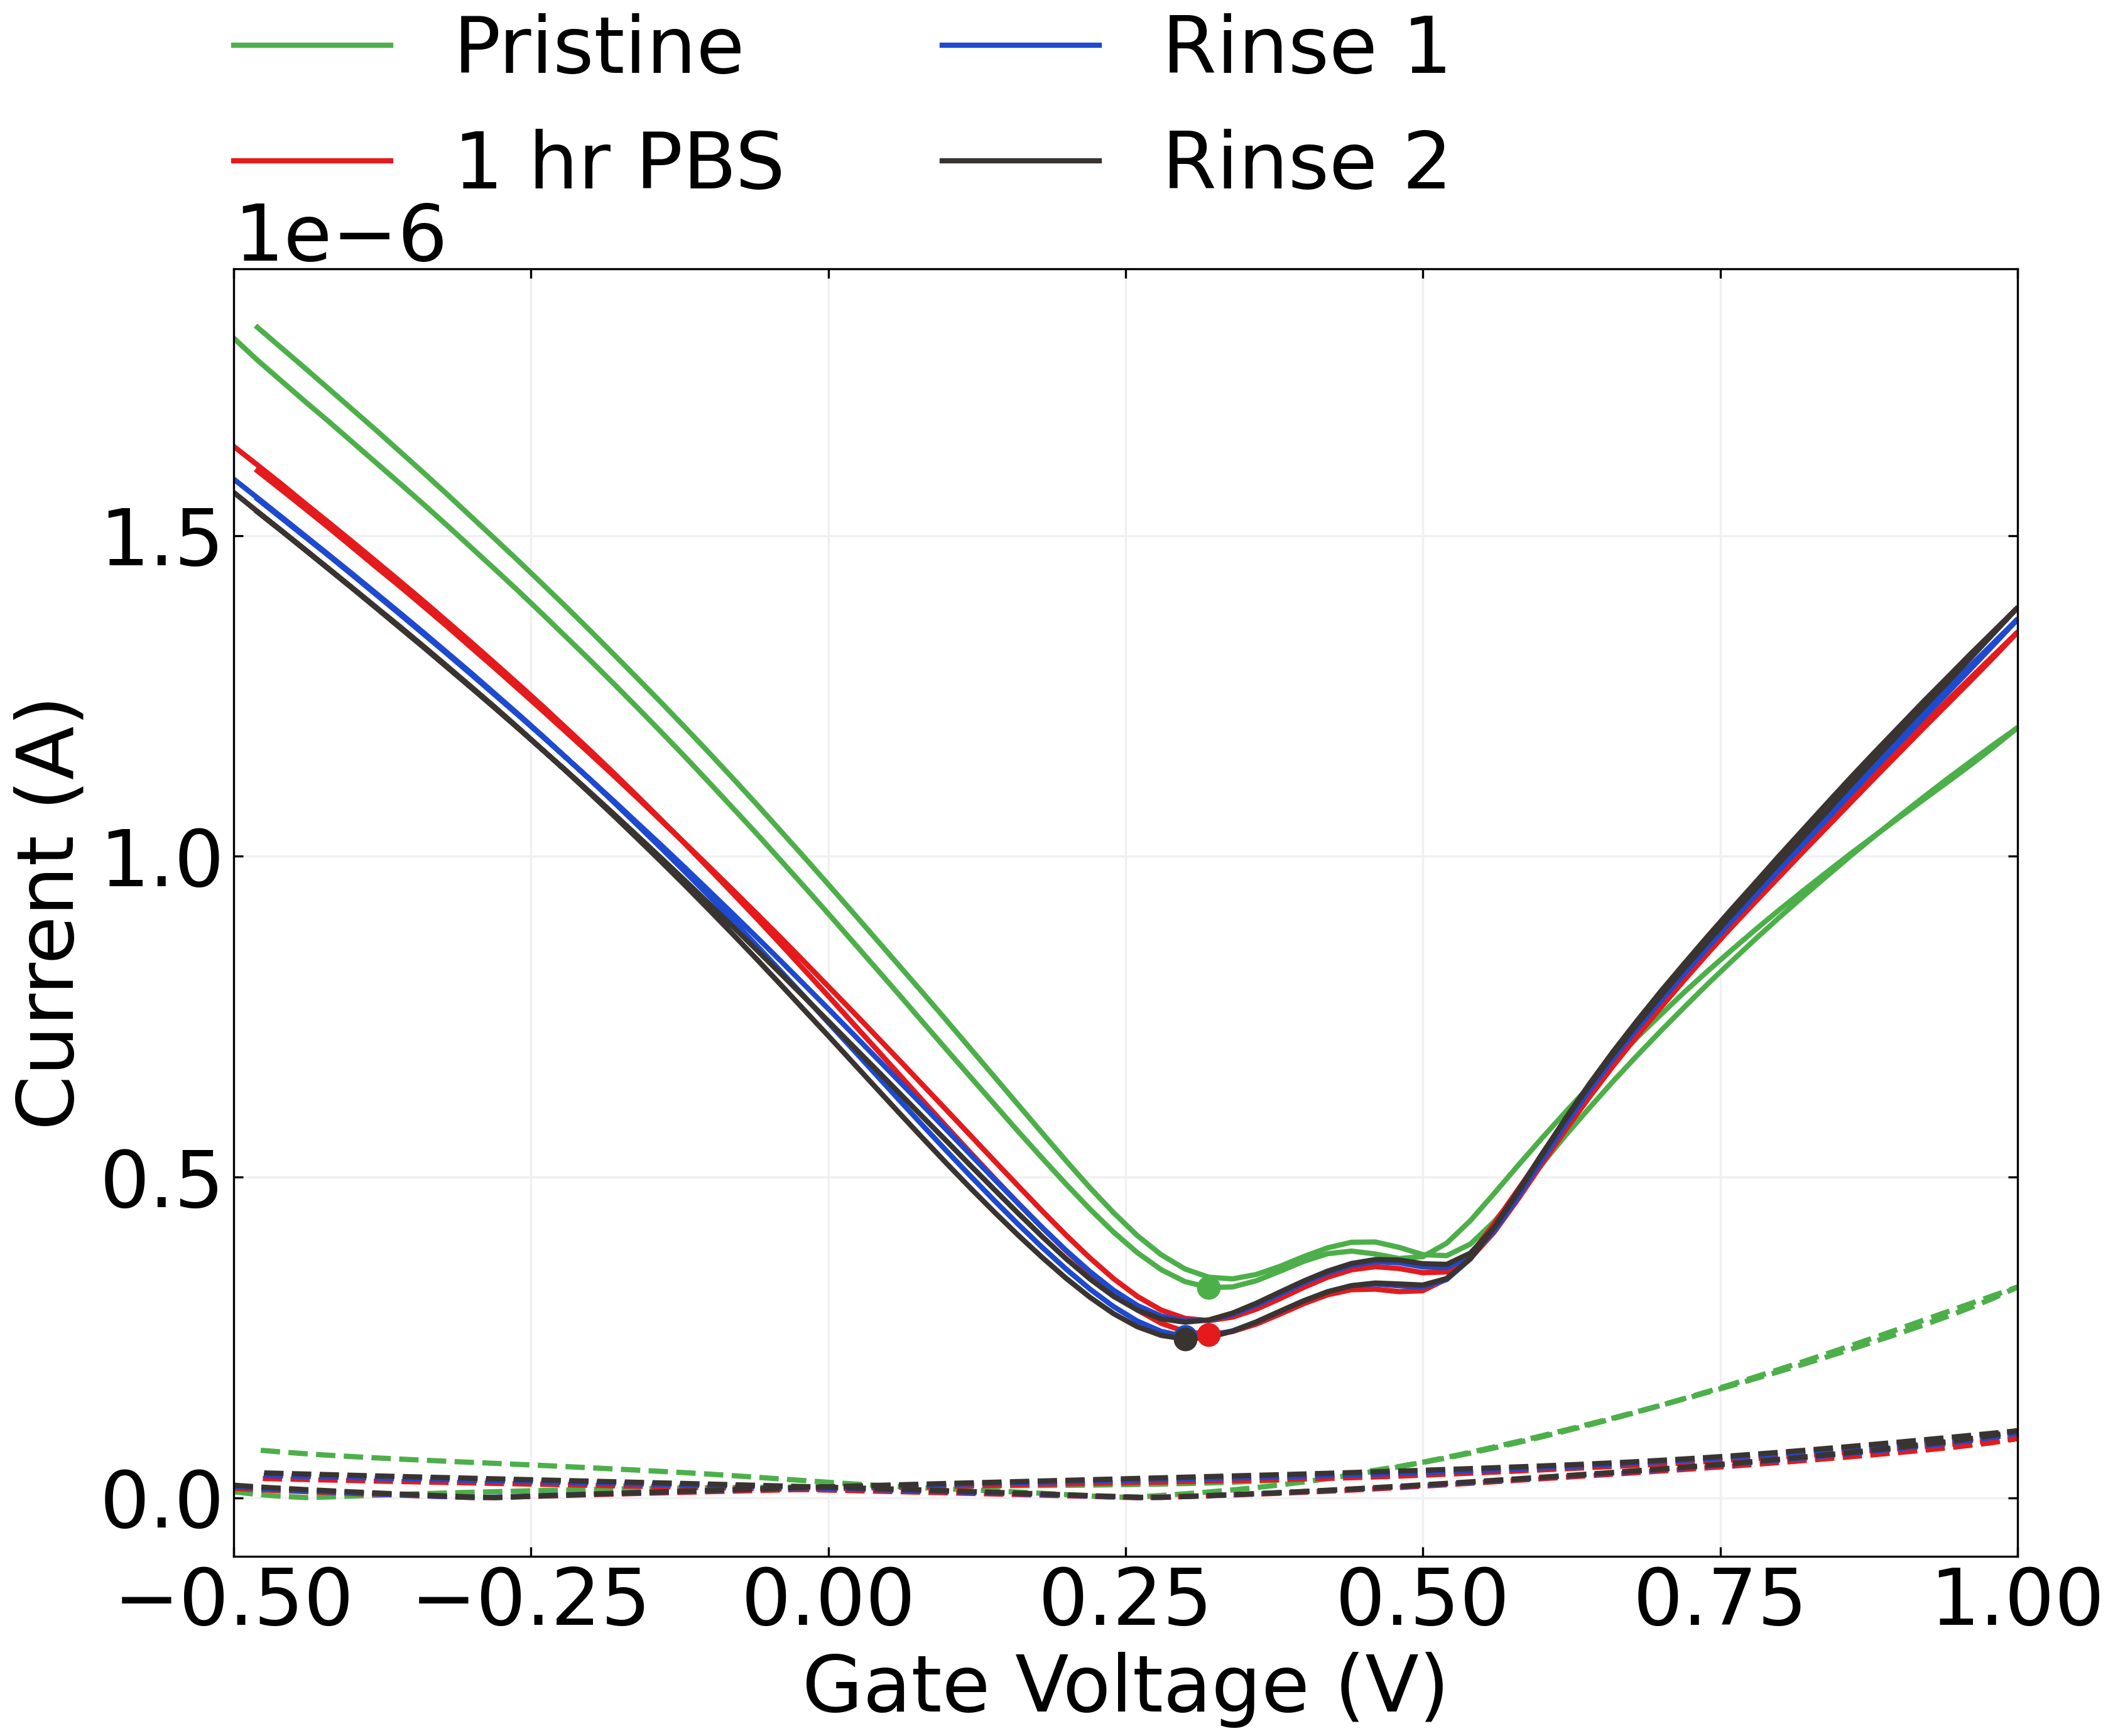
\includegraphics{figures/ch6/JGQ00D6_ch3_absolute_values_with_gate_current.png}

}

}

\subcaption{\label{fig-graphene-transfer-comparison-2}}
\end{minipage}%

\caption{\label{fig-pristine-graphene}These figures show liquid-gated
transfer characteristics of channels from two AZ\(^\circledR\) 1518
encapsulated graphene devices. The characteristics of working device
channels upon initial exposure to 1XPBS are shown in (a) and (b). The
transfer characteristics of channel 1 in (a) and channel 5 in (b) after
various degrees of exposure to 1XPBS are shown in (c) and (d)
respectively, with each transfer sweep numbered in the order the sweeps
were taken. The dashed lines correspond to measurements of gate leakage
current.}

\end{figure}

Graphene field-effect transistor devices were electrically characterised
in the manner described in \textbf{?@sec-electrical-characterisation}
and analysed using the Python code discussed in
Section~\ref{sec-field-effect-transistor-analysis}.

Figure~\ref{fig-pristine-graphene} shows the liquid-gated transfer
characteristics of two graphene devices. These devices were fabricated
prior to Jun 2021. Both devices exhibit the ambipolar characteristics
typical of liquid-gated graphene devices
\autocite{Heller2009a,Heller2010,Xia2010,Kireev2017}. As with the carbon
nanotube network devices, leakage current remained below \(\sim\) 1
\(\times\) \(10^{-7}\) V across both the forward and reverse sweep.
Hysteresis between the forward and reverse sweep is caused by trapping
of charge within and on the surface of the SiO\(_{2}\) dielectric
\autocite{Bartolomeo2011}. The major Dirac point for these devices is
slightly to the right of V\(_{\textrm{Dirac}} \approxeq\) 0 V, which
indicates \(p\)-doping of the channel. This slight \(p\)-doping is
likely a result of a adsorption of oxygen and water from the air and
residue resist from photolithography
\autocite{Cheng2011,Shin2012,Kireev2017}.

Some devices exhibited a double-minima feature, indicating the presence
of two Dirac points. This effect arises due to doping of graphene by the
metal contacts. In shorter length channels, metal doping affects the
entire channel length, leading to a consistent Fermi level and a single
Dirac point. However, for longer channel lengths like ours, the doping
effect from metal contact no longer reaches the entire channel, leading
to a difference in Fermi level between the graphene in the channel and
graphene under the metal contact. The difference in Fermi levels results
in the presence of a second Dirac point
\autocite{Bartolomeo2011,Feng2014,Peng2018}. The global minimum of the
transfer characteristic can be referred to as the `major' Dirac point.

Figure~\ref{fig-pristine-graphene} also shows the effect of 1XPBS on the
graphene channels. The channels were measured on exposure to 1XPBS,
after exposure to 1XPBS for one hour, and after the device surface was
rinsed and 1XPBS was replaced in the well one time, two times and three
times successively. A slight negative shift of the major Dirac point was
observed. This effect is possibly a result of gate bias stress, where
successive transfer sweeps introduce charge traps to the graphene layer
and alters the current level at a given gate voltage
\autocite{Bargaoui2018,Noyce2019}. Alternatively, Kireev \emph{et al.}
found that a series of liquid-gated sweeps also reduced the size of the
second Dirac point, and suggested that it indicated the gate current was
removing atmospheric contaminants from the graphene surface via current
annealing \autocite{Kireev2017}. This could be explained as the removal
of contaminants causing improved contact between the metal and graphene
surface, and thus increasing metal doping and consistency of the Fermi
level across the channel. If the contaminants removed are \(p\)-dopants,
then this effect could also explain the negative shift of the major
Dirac point.

\hypertarget{tbl-graphene-parameters}{}
\begin{longtable}[]{@{}
  >{\raggedright\arraybackslash}p{(\columnwidth - 6\tabcolsep) * \real{0.3288}}
  >{\centering\arraybackslash}p{(\columnwidth - 6\tabcolsep) * \real{0.2192}}
  >{\centering\arraybackslash}p{(\columnwidth - 6\tabcolsep) * \real{0.2603}}
  >{\centering\arraybackslash}p{(\columnwidth - 6\tabcolsep) * \real{0.1918}}@{}}
\caption{\label{tbl-graphene-parameters}Average on-off ratio and major
Dirac point voltage for AZ® 1518 encapsulated liquid-gated graphene
transistor channels at various stages of exposure to 1XPBS. Electrical
characteristics were taken of 6 channels total, three channels from each
of two devices.}\tabularnewline
\toprule\noalign{}
\begin{minipage}[b]{\linewidth}\raggedright
\end{minipage} & \begin{minipage}[b]{\linewidth}\centering
1XPBS: Initial
\end{minipage} & \begin{minipage}[b]{\linewidth}\centering
1XPBS: After 1 hr
\end{minipage} & \begin{minipage}[b]{\linewidth}\centering
1XPBS: Rinse
\end{minipage} \\
\midrule\noalign{}
\endfirsthead
\toprule\noalign{}
\begin{minipage}[b]{\linewidth}\raggedright
\end{minipage} & \begin{minipage}[b]{\linewidth}\centering
1XPBS: Initial
\end{minipage} & \begin{minipage}[b]{\linewidth}\centering
1XPBS: After 1 hr
\end{minipage} & \begin{minipage}[b]{\linewidth}\centering
1XPBS: Rinse
\end{minipage} \\
\midrule\noalign{}
\endhead
\bottomrule\noalign{}
\endlastfoot
On-Off Ratio (arb.) & 5.1 ± 0.3 & 5.0 ± 0.7 & 5.0 ± 0.6 \\
Dirac Point Voltage (V) & 0.28 ± 0.04 & 0.31 ± 0.03 & 0.28 ± 0.02 \\
\end{longtable}

Table~\ref{tbl-graphene-parameters} shows the on-off ratio and major
Dirac point voltage of the graphene devices. Apart from the
previously-mentioned slight negative shift of the major Dirac point,
these values were highly consistent before and after exposure to 1XPBS.

\hypertarget{sec-dummy-sensing}{%
\section{Aqueous Sensing of Phosphate Buffered Saline
Concentration}\label{sec-dummy-sensing}}

\hypertarget{sec-baseline-drift}{%
\subsection{Control Series and Baseline
Drift}\label{sec-baseline-drift}}

\hypertarget{tbl-threshold-voltages}{}
\begin{longtable}[]{@{}lrrrrrr@{}}
\caption{\label{tbl-threshold-voltages}The threshold voltages \(V_{th}\)
of each working channel of a steam-deposited device, and the difference
between each \(V_{th}\) and the mean device threshold voltage
\(V_{th, mean}\).\\
}\tabularnewline
\toprule\noalign{}
Channels & CH1 & CH2 & CH3 & CH5 & CH6 & CH7 \\
\midrule\noalign{}
\endfirsthead
\toprule\noalign{}
Channels & CH1 & CH2 & CH3 & CH5 & CH6 & CH7 \\
\midrule\noalign{}
\endhead
\bottomrule\noalign{}
\endlastfoot
Threshold voltage (mV) & 160 & 150 & 130 & 140 & 180 & 140 \\
Relative to mean (mV) & 10 & 0 & -20 & -10 & 30 & -10 \\
\end{longtable}

To verify the sensitivity of the fabricated field-effect transistors and
therefore verify their suitability for sensing, control measurements
replicating a typical sensing experiment were taken before
functionalising the channels of a carbon nanotube network device. The
first step to verifying device suitability was ensuring the device
showed no response to 1XPBS. This sequence is referred to in this thesis
as the `PBS control series'. The PDMS well contained 80 \(\mu\)L 1X PBS
at 0 s. The PBS control series ran over the first 1800 s, with
20\(\mu\)L phosphate buffer saline (1XPBS) additions at 100 s, 200 s and
300 s, and 20\(\mu\)L subtractions at 400 s, 500 s and 600 s. The device
was left untouched over the next 1200 s to allow the current level to
settle. The gate voltage was held at \(V_g\) = 0 V.

Figure~\ref{fig-transfer-sweeps} shows the transfer sweeps of the six
working channels of a steam-assisted surfactant-deposited carbon
nanotube field-effect transistor measured using the NI PXIe. The device
was fabricated on a substrate with a 300 nm SiO\(_{2}\) layer, the
carbon nanotube film was deposited using the steam-assisted surfactant
method and encapsulated with AZ\(^\circledR\) 1518 before measurement.
The central feature in the transfer characteristics of channels 1 and 7
are absolute-value measurements of negative current. These are
unphysical measurements due to equipment error, and can be considered as
regions where zero current passes through the channel. The threshold
voltages of the channels are shown in
Table~\ref{tbl-threshold-voltages}. Table~\ref{tbl-threshold-voltages}
also shows the difference between the threshold voltage of each channel
and the mean threshold voltage of the device. The mean threshold voltage
was \(V_{th}\) = \(150 \pm 20\) mV. As discussed previously, the
electrical characteristics are highly consistent between the channels
due to the film deposition method used.

\begin{figure}

\begin{minipage}[t]{0.45\linewidth}

{\centering 

\raisebox{-\height}{

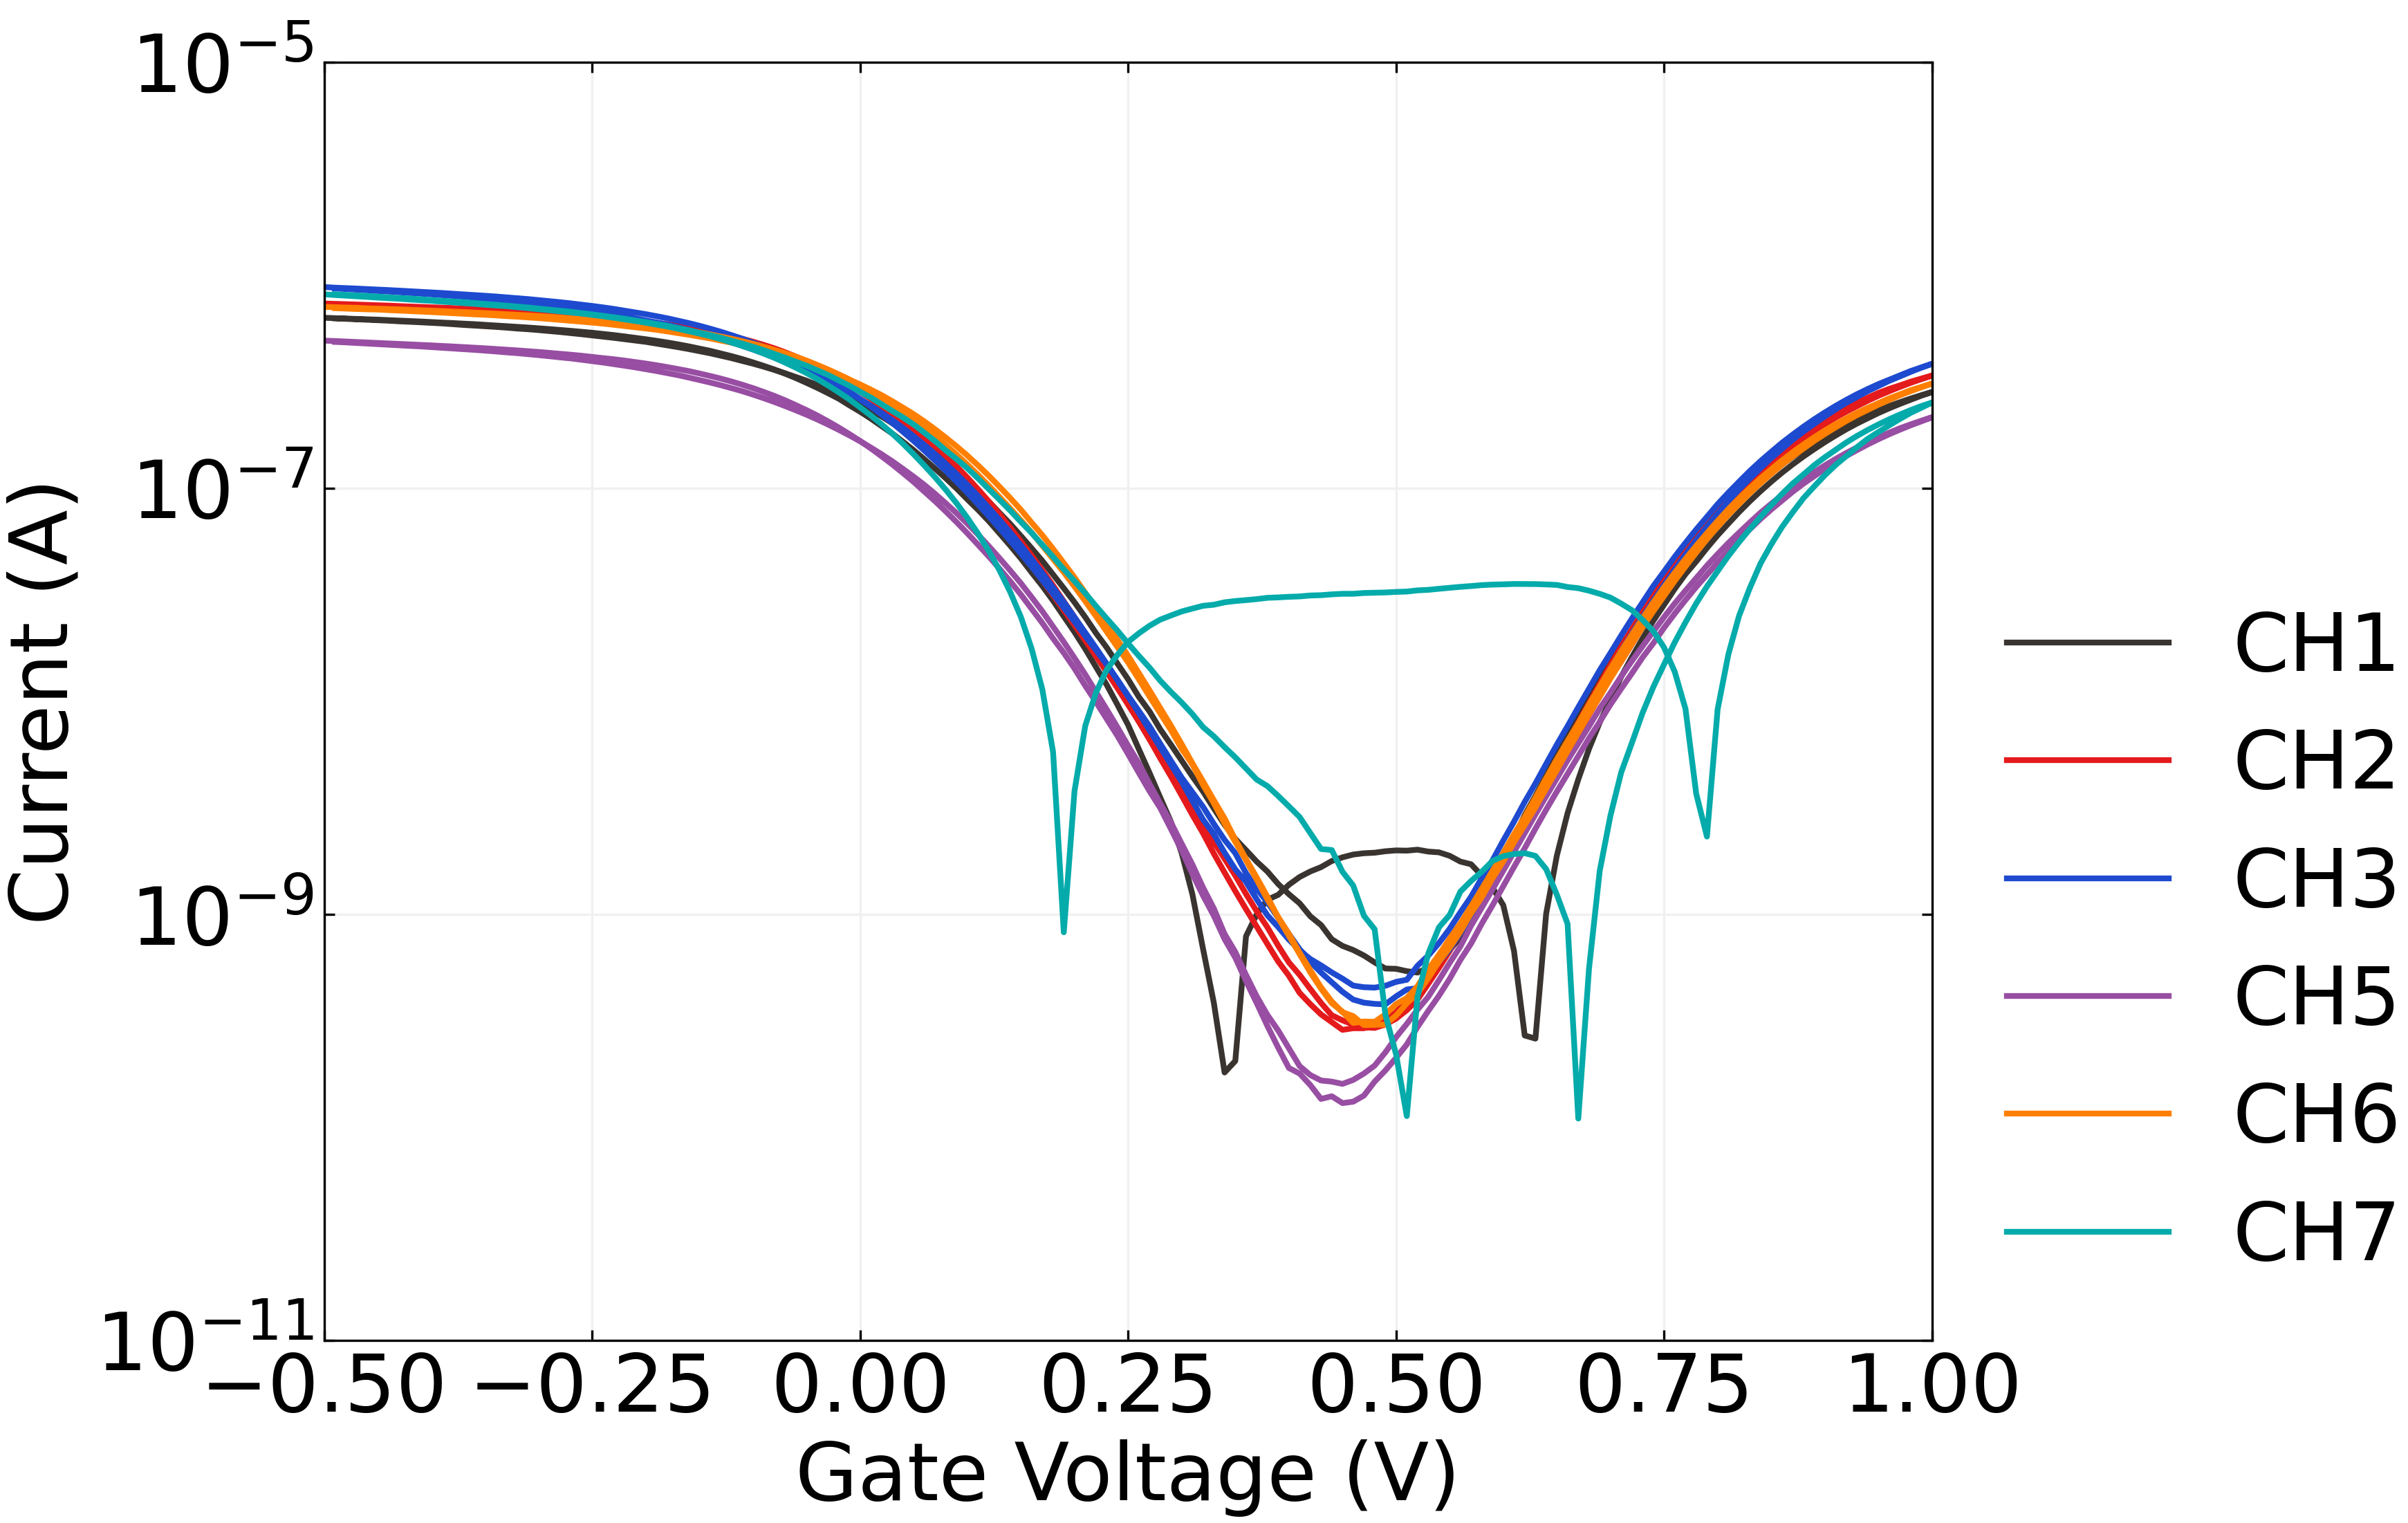
\includegraphics{figures/ch6/NTQ31C1_pristine_TXLG02_230322.png}

}

}

\subcaption{\label{fig-transfer-sweeps}}
\end{minipage}%
%
\begin{minipage}[t]{0.05\linewidth}

{\centering 

~

}

\end{minipage}%
%
\begin{minipage}[t]{0.50\linewidth}

{\centering 

\raisebox{-\height}{

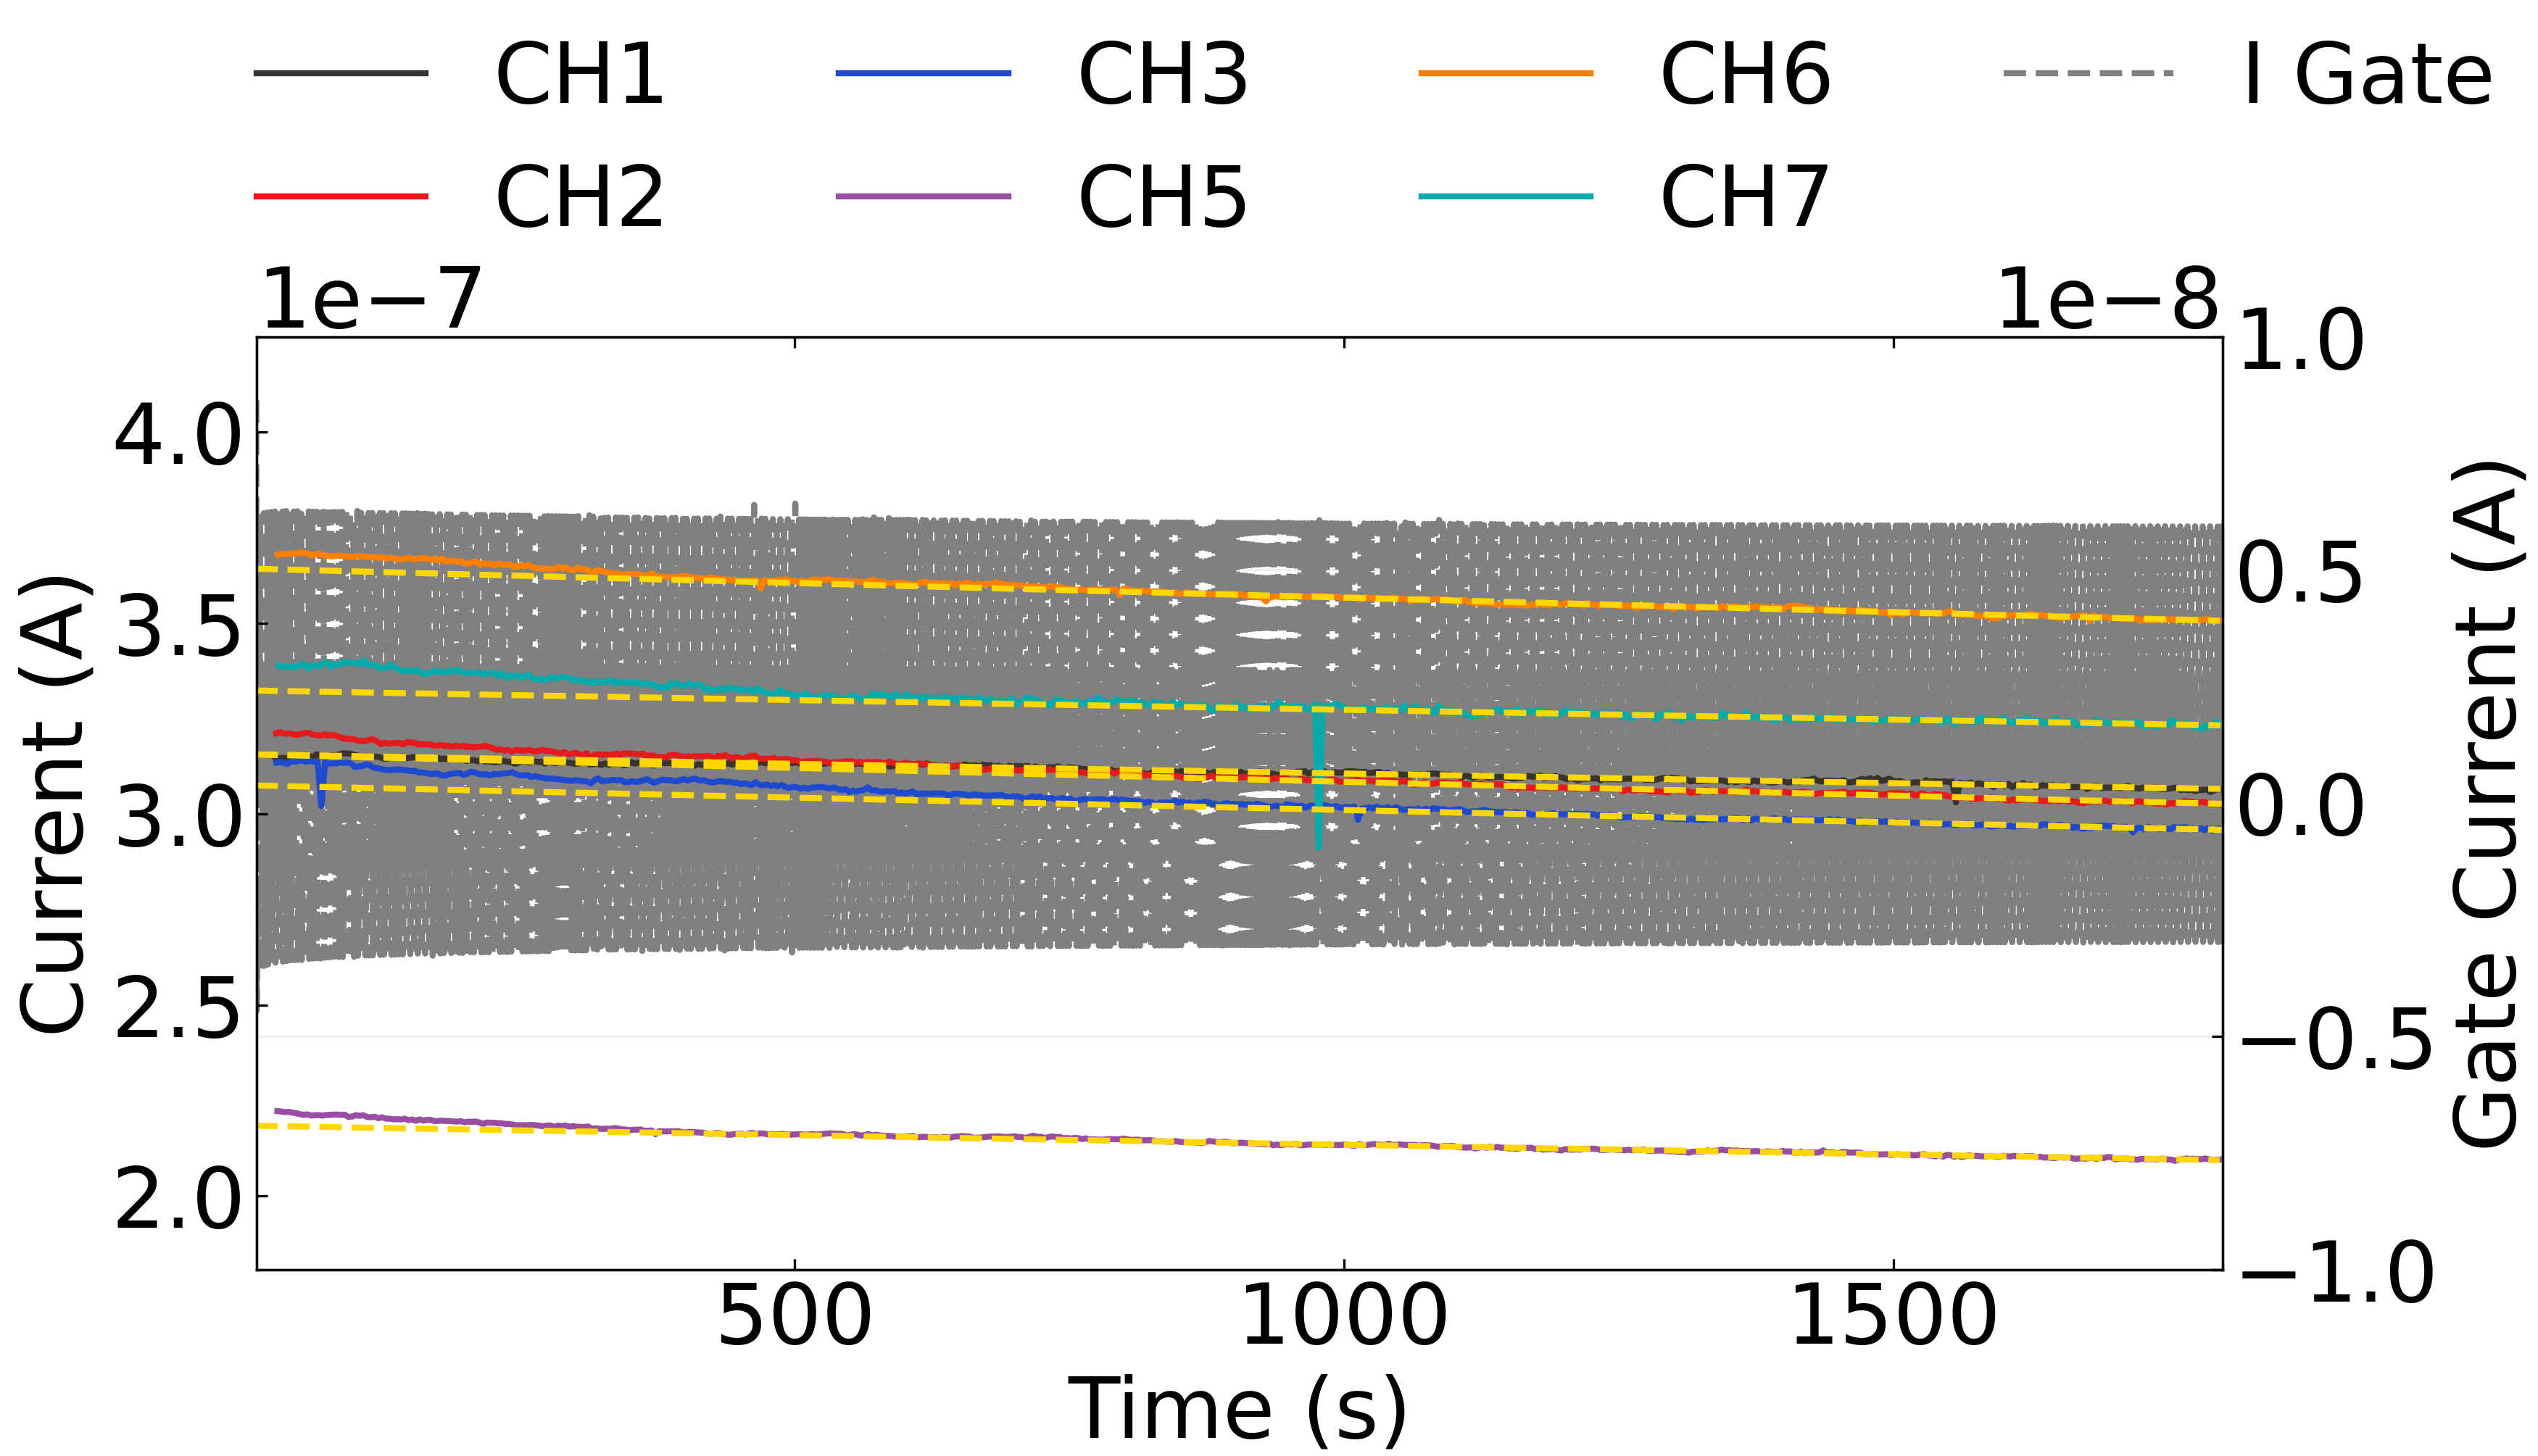
\includegraphics{figures/ch6/NTQ31C1_pristine_saltconc_sample_230324_control.png}

}

}

\subcaption{\label{fig-linear-fit}}
\end{minipage}%
\newline
\begin{minipage}[t]{0.28\linewidth}

{\centering 

~

}

\end{minipage}%
%
\begin{minipage}[t]{0.45\linewidth}

{\centering 

\raisebox{-\height}{

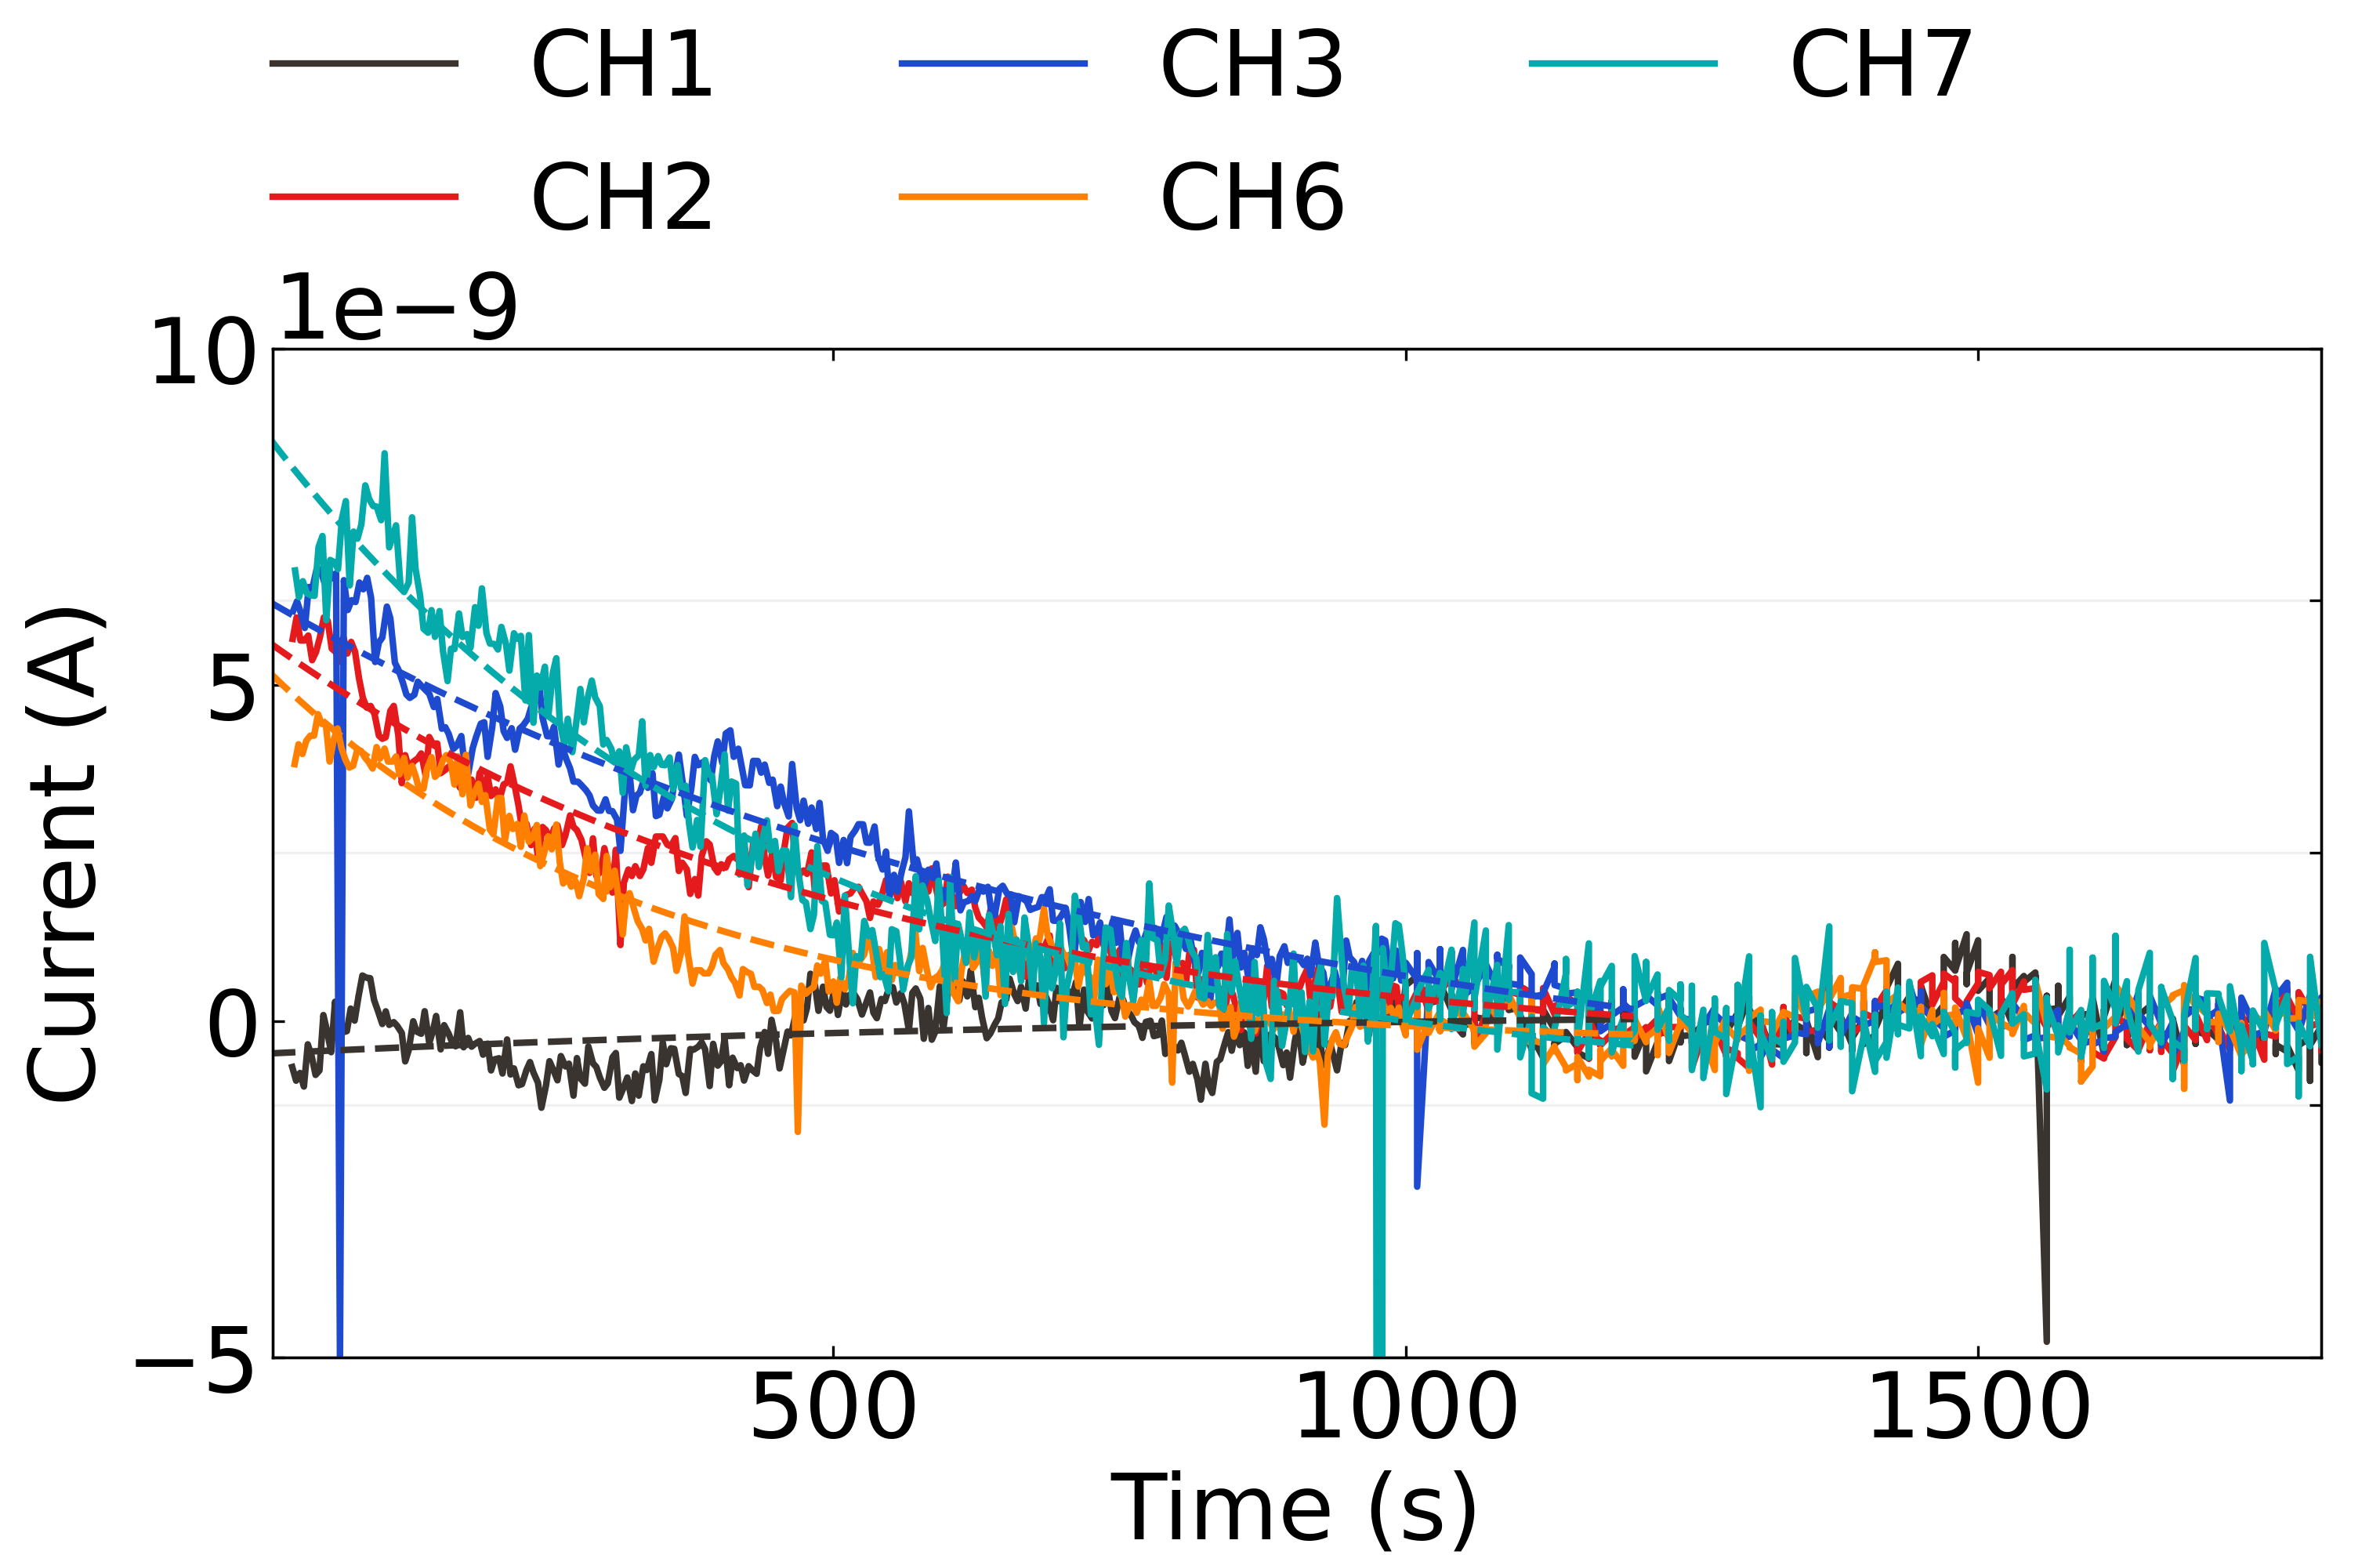
\includegraphics{figures/ch6/NTQ31C1_pristine_saltconc_sample_230324_linear_fit_exp.png}

}

}

\subcaption{\label{fig-exp-fit}}
\end{minipage}%
%
\begin{minipage}[t]{0.28\linewidth}

{\centering 

~

}

\end{minipage}%

\caption{\label{fig-salt-conc-control-series}The transfer
characteristics in (a) were taken of the steam-deposited carbon nanotube
field-effect transistor used here for an example of salt concentration
sensing. The absolute values of measurements are shown, so that negative
values resulting from measurement error can be visualised. Linear fits
to the PBS control series from each channel from 1200 s onwards are
shown in (b), while exponential fits to the PBS control series from
\(0-1200\) with the linear fit subtracted are shown in (c). No
significant response to PBS additions are seen at any of the addition
times from 100 s - 600 s.}

\end{figure}

Figure~\ref{fig-linear-fit} shows the PBS control series corresponding
to each device channel alongside gate current. In both series, there is
no clear stepwise response to any addition or subtraction of 1XPBS. Gate
leakage current remains negligible across the entire control series,
with no change in response to 1XPBS additions. The current has a period
of faster decay followed by slower baseline drift, similar to
observations by Lin \emph{et al.} and more recently Noyce \emph{et al.}
for parallel arrangements of single carbon nanotubes in air or vacuum
\autocite{Lin2006,Noyce2019}. This effect results from changes in the
occupancy of charge traps in and around the substrate and carbon
nanotubes. The magnitude of baseline drift is lower for our devices than
for those characterised by Noyce \emph{et al.}, which may be a result of
numerous device and setup differences which affect the presence of
charge traps. These differences include liquid-gating instead of
back-gated, the use of a network of carbon nanotubes instead of single
nanotubes, a different channel length, the use of a 300 nm instead of 90
nm SiO\(_2\) layer, and the use of an asymmetric, liquid-gated transfer
sweep over a shorter voltage range to characterise devices before each
control series was measured \autocite{Noyce2019}.

\hypertarget{tbl-linear-fits}{}
\begin{longtable}[]{@{}lllllll@{}}
\caption{\label{tbl-linear-fits}The coefficients of linear fits to the
PBS control series of each channel between \(1200-1800\) s, where
\(c_1\) is the gradient and \(c_2\) is the constant term.\\
}\tabularnewline
\toprule\noalign{}
Channels & CH1 & CH2 & CH3 & CH5 & CH6 & CH7 \\
\midrule\noalign{}
\endfirsthead
\toprule\noalign{}
Channels & CH1 & CH2 & CH3 & CH5 & CH6 & CH7 \\
\midrule\noalign{}
\endhead
\bottomrule\noalign{}
\endlastfoot
\(c_1\) (pA/s) & -5.1±0.2 & -7.2±0.1 & -6.5±0.1 & -5.0±0.1 & -7.6±0.1 &
-5.1±0.2 \\
\(c_2\) (\(\mu\)A) & 0.316 & 0.316 & 0.308 & 0.218 & 0.364 & 0.332 \\
\end{longtable}

\hypertarget{tbl-exp-fits}{}
\begin{longtable}[]{@{}llllll@{}}
\caption{\label{tbl-exp-fits}The coefficients of exponential fits to the
PBS control series of each channel between \(0-1200\) s, after the
linear fit has been subtracted, where \(I_0\) is the gradient and
\(\tau\) is the time constant.\\
}\tabularnewline
\toprule\noalign{}
Channels & CH1 & CH2 & CH3 & CH6 & CH7 \\
\midrule\noalign{}
\endfirsthead
\toprule\noalign{}
Channels & CH1 & CH2 & CH3 & CH6 & CH7 \\
\midrule\noalign{}
\endhead
\bottomrule\noalign{}
\endlastfoot
\(I_0\) (nA) & \(-0.66\pm0.26\) & \(6.21\pm0.09\) & \(7.84\pm0.41\) &
\(5.67\pm0.11\) & \(9.82\pm0.47\) \\
\(\tau\) (s) & \(800\pm750\) & \(500\pm30\) & \(790\pm100\) &
\(330\pm20\) & \(440\pm70\) \\
\end{longtable}

As a first approximation to the longer time constant exponentials
discussed by Noyce \emph{et al.} \autocite{Noyce2019}, linear fits were
performed on each PBS control series from \(1200-1800\) s. These linear
fits are shown by the dashed yellow lines in
Figure~\ref{fig-linear-fit}. The parameters from each fit in
Figure~\ref{fig-linear-fit} are shown in Table~\ref{tbl-linear-fits},
where \(I = c_1t + c_2\). The fits for channels 1, 5 and 7 are all in
parallel within error. The gradient value for each fit in
Figure~\ref{fig-linear-fit} is reasonably consistent between all
channels, all falling within a 2.6 pA/s range. When the long-term linear
fits were subtracted from the raw data, the remaining dataset followed a
exponential decay trend for both control series.

Figure~\ref{fig-exp-fit} shows exponential fits to the remaining curve
from \(0-1200\) s, which was successful for all channels except channel
5. The parameters from each fit are shown in Table~\ref{tbl-exp-fits},
where \(I = I_0\exp(-t/\tau)\). Any constant term \(I_C\) resulting from
the fit was negligible and so could be neglected. The exponential fits
had characteristic time constants \(\tau\) ranging between \(300 - 800\)
s. This result indicates 1800 s is a sufficient length of time for this
short-term baseline drift to decay almost completely for the channels
with smaller time constants. However, it means that for some channels, a
control sequence of up to 4000 s may be required for this term to be
neglected. The exponential term for channel 1 has a amplitude close to
zero, indicating the channel has low net trapped charge. It is unclear
why the behaviour of this channel is signficantly different from the
others.

From this analysis it appears that the baseline drift for the
liquid-gated carbon nanotube devices can be accurately approximated as a
combination of a exponential and linear term. The lack of response to
1XPBS at any of the six PBS addition and removal times gives us
confidence that this is a stable baseline which can be used for reliable
chemical sensing. Furthermore, after \(\sim 800\) s the baseline drift
can be reasonably approximated as linear, with a small gradient of less
than -10 pA/s. The slow change of current means that it becomes easier
to distinguish responses due to analyte addition. It can therefore be
concluded that the 1800 s length of the PBS control series is
appropriate for minimising baseline drift for more reliable sensing.

\hypertarget{sec-salt-conc-series}{%
\subsection{Sensing Series}\label{sec-salt-conc-series}}

A salt concentration sensing series were performed from 1800 s onwards,
directly after the PBS control series. The responses to successive
dilutions of the liquid-gate electrolyte were recorded to confirm the
fabricated devices were sensitive to small environmental changes in
their pristine state, to check for spurious signals, and to ensure gate
current leakage or other confounding factors were not contributing to
sensing responses. The PDMS well contained 80 \(\mu\)L 1X PBS at 1800 s.
During the series, successive additions of deionised water were made to
reduce the concentration of PBS in the well. An initial 1X PBS addition
was performed at 2100s, to confirm no changes occurred during the PBS
control series that would interfere with sensing. All additions to the
well in the sensing series and resulting changes to the PBS
concentration in the well are shown in Table~\ref{tbl-salt-conc-series}.

\hypertarget{tbl-salt-conc-series}{}
\begin{longtable}[t]{lcccccc}
\caption{\label{tbl-salt-conc-series}This table shows the times at which 20 µL additions were made to the
PDMS well, with 300 s between each addition. The concentration in the
well after each addition and the change in concentration after each
addition are also shown. The well contained 80 µL of 1X PBS at 1800 s. }\tabularnewline

\toprule
\multicolumn{1}{c}{ } & \multicolumn{1}{c}{1X PBS Addition} & \multicolumn{5}{c}{DI Water Additions} \\
\cmidrule(l{3pt}r{3pt}){2-2} \cmidrule(l{3pt}r{3pt}){3-7}
 &  &  &  &  &  & \\
\midrule
Time (s) & 2100 & 2400 & 2700 & 3000 & 3300 & 3600\\
Final PBS volume (µL) & 100 & 120 & 140 & 160 & 180 & 200\\
Final PBS concentration & 1X & 0.83X & 0.71X & 0.63X & 0.56X & 0.50X\\
Δ PBS concentration & 0 & -0.17X & -0.12X & -0.09X & -0.07X & -0.06X\\
\bottomrule
\end{longtable}

\begin{figure}

\begin{minipage}[t]{0.50\linewidth}

{\centering 

\raisebox{-\height}{

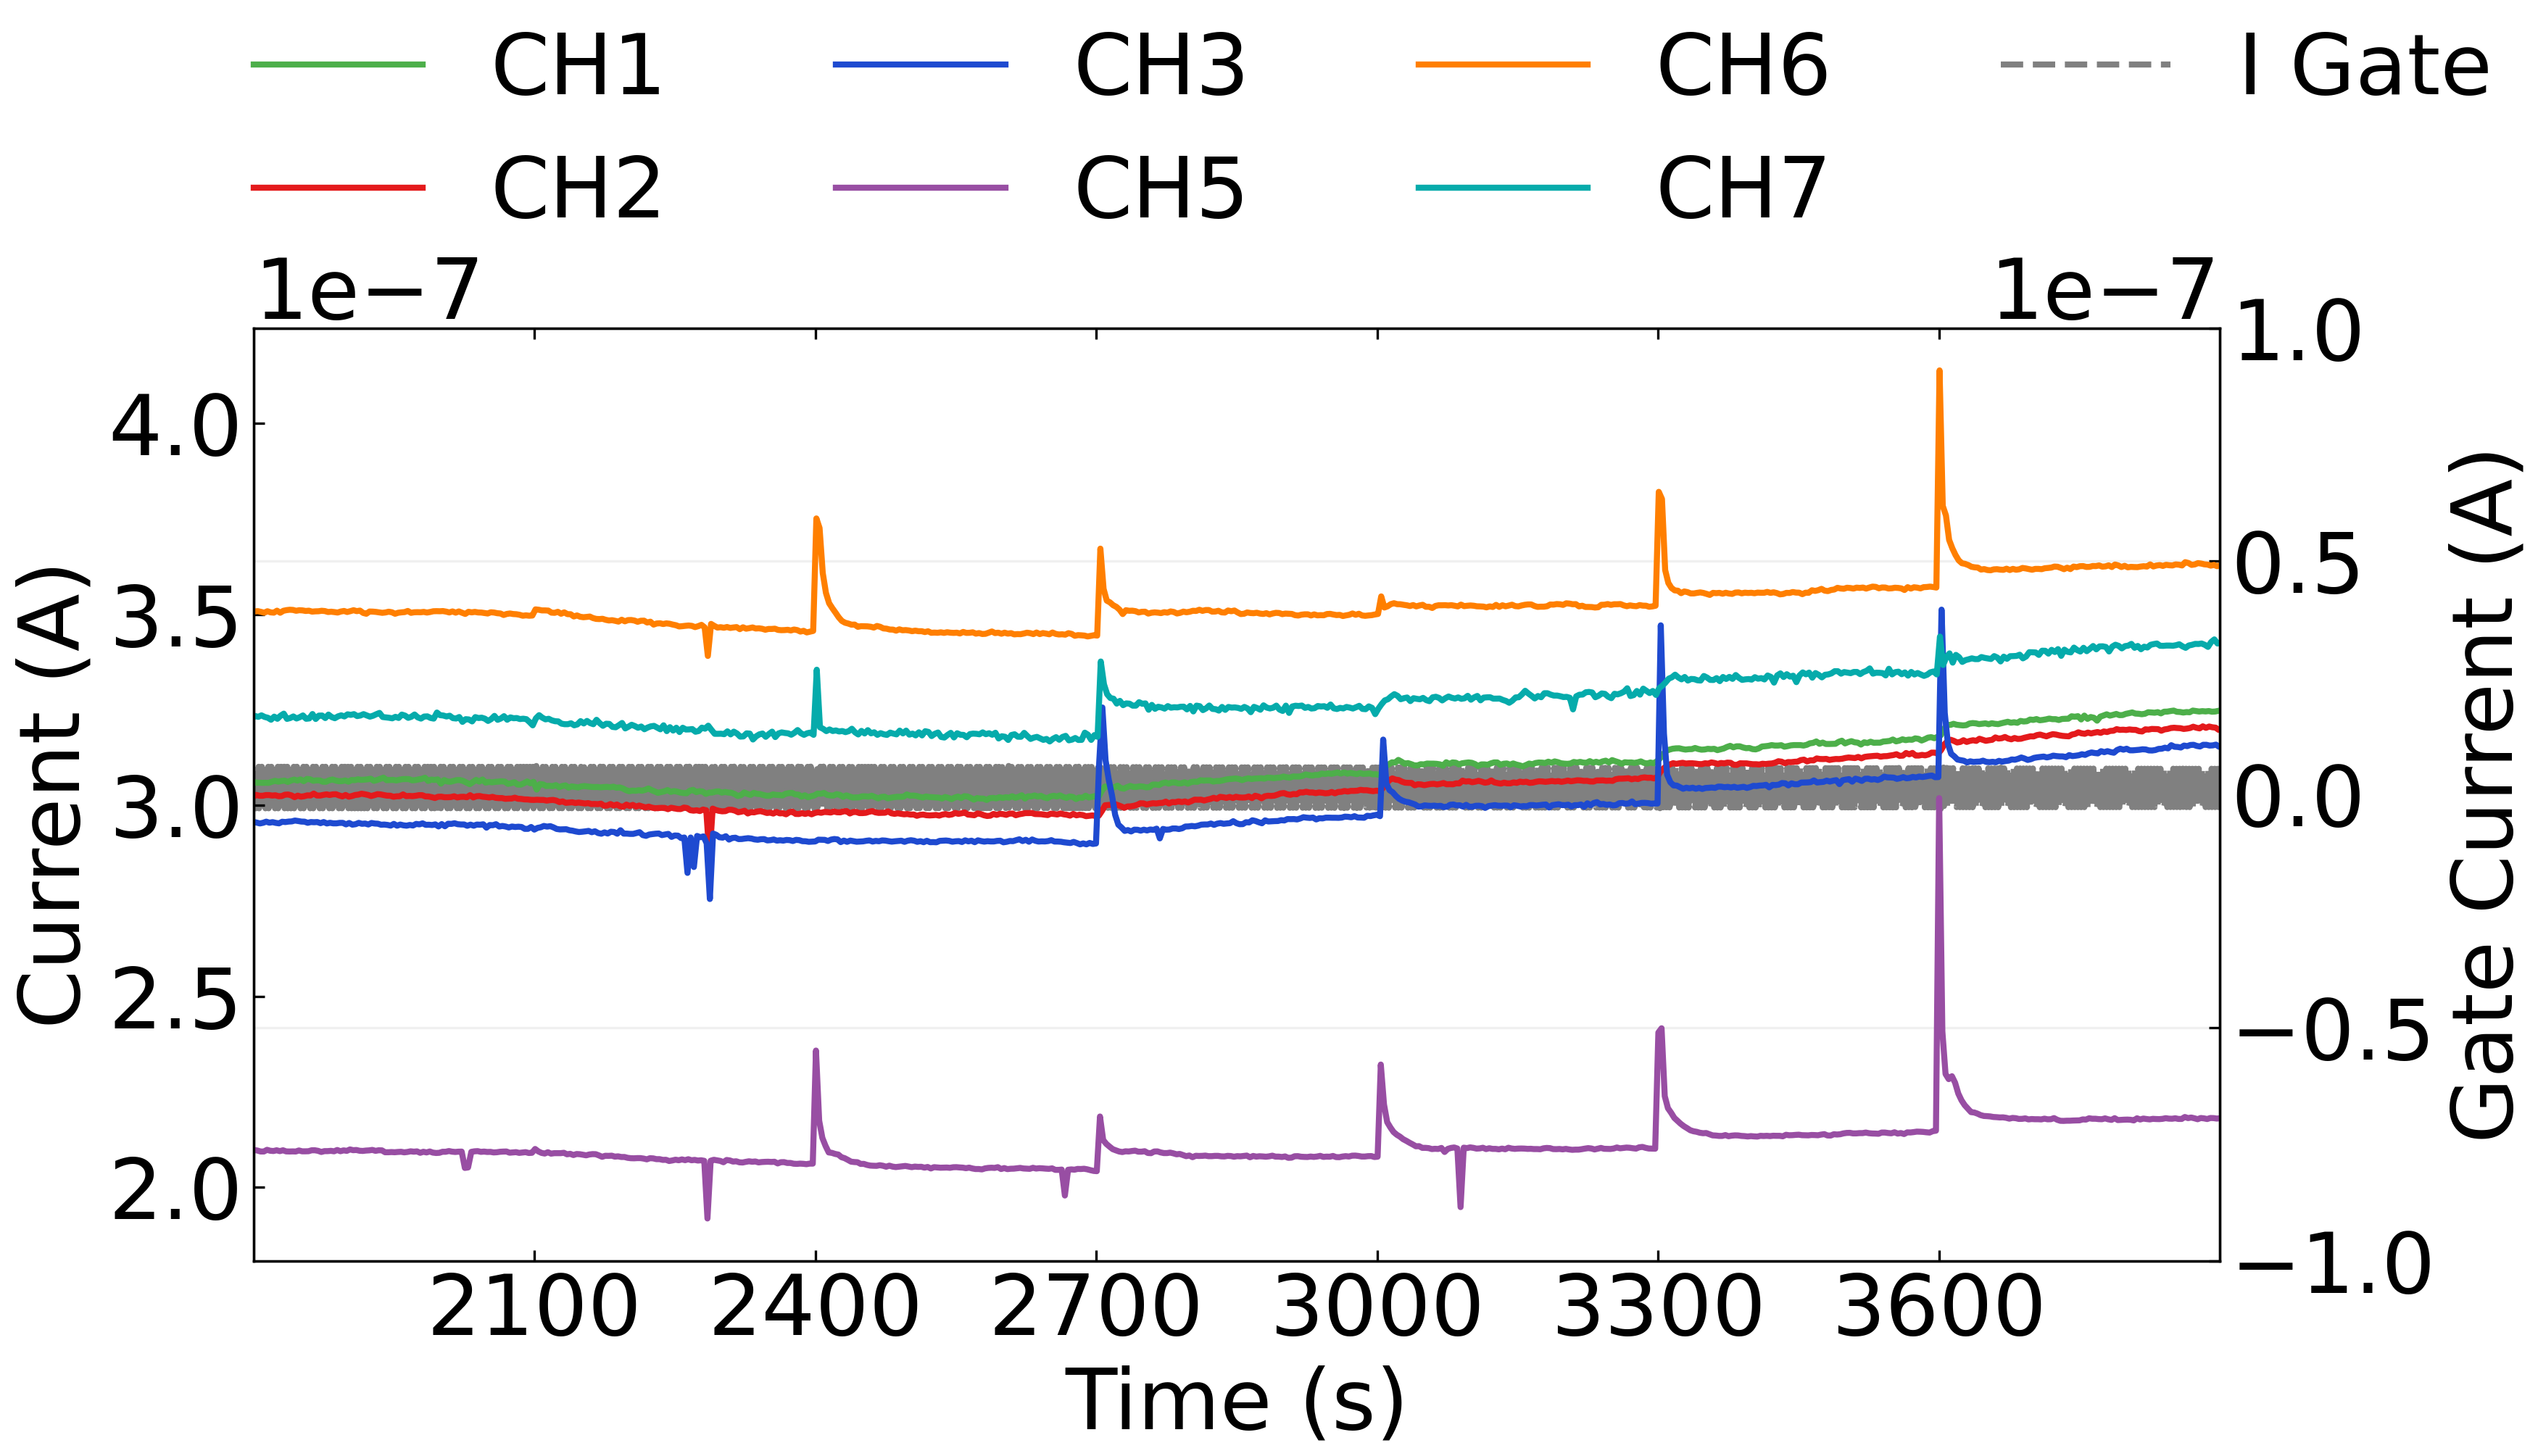
\includegraphics{figures/ch6/NTQ31C1_pristine_saltconc_sample_230324.png}

}

}

\subcaption{\label{fig-salt-conc-no-norm}}
\end{minipage}%
%
\begin{minipage}[t]{0.50\linewidth}

{\centering 

\raisebox{-\height}{

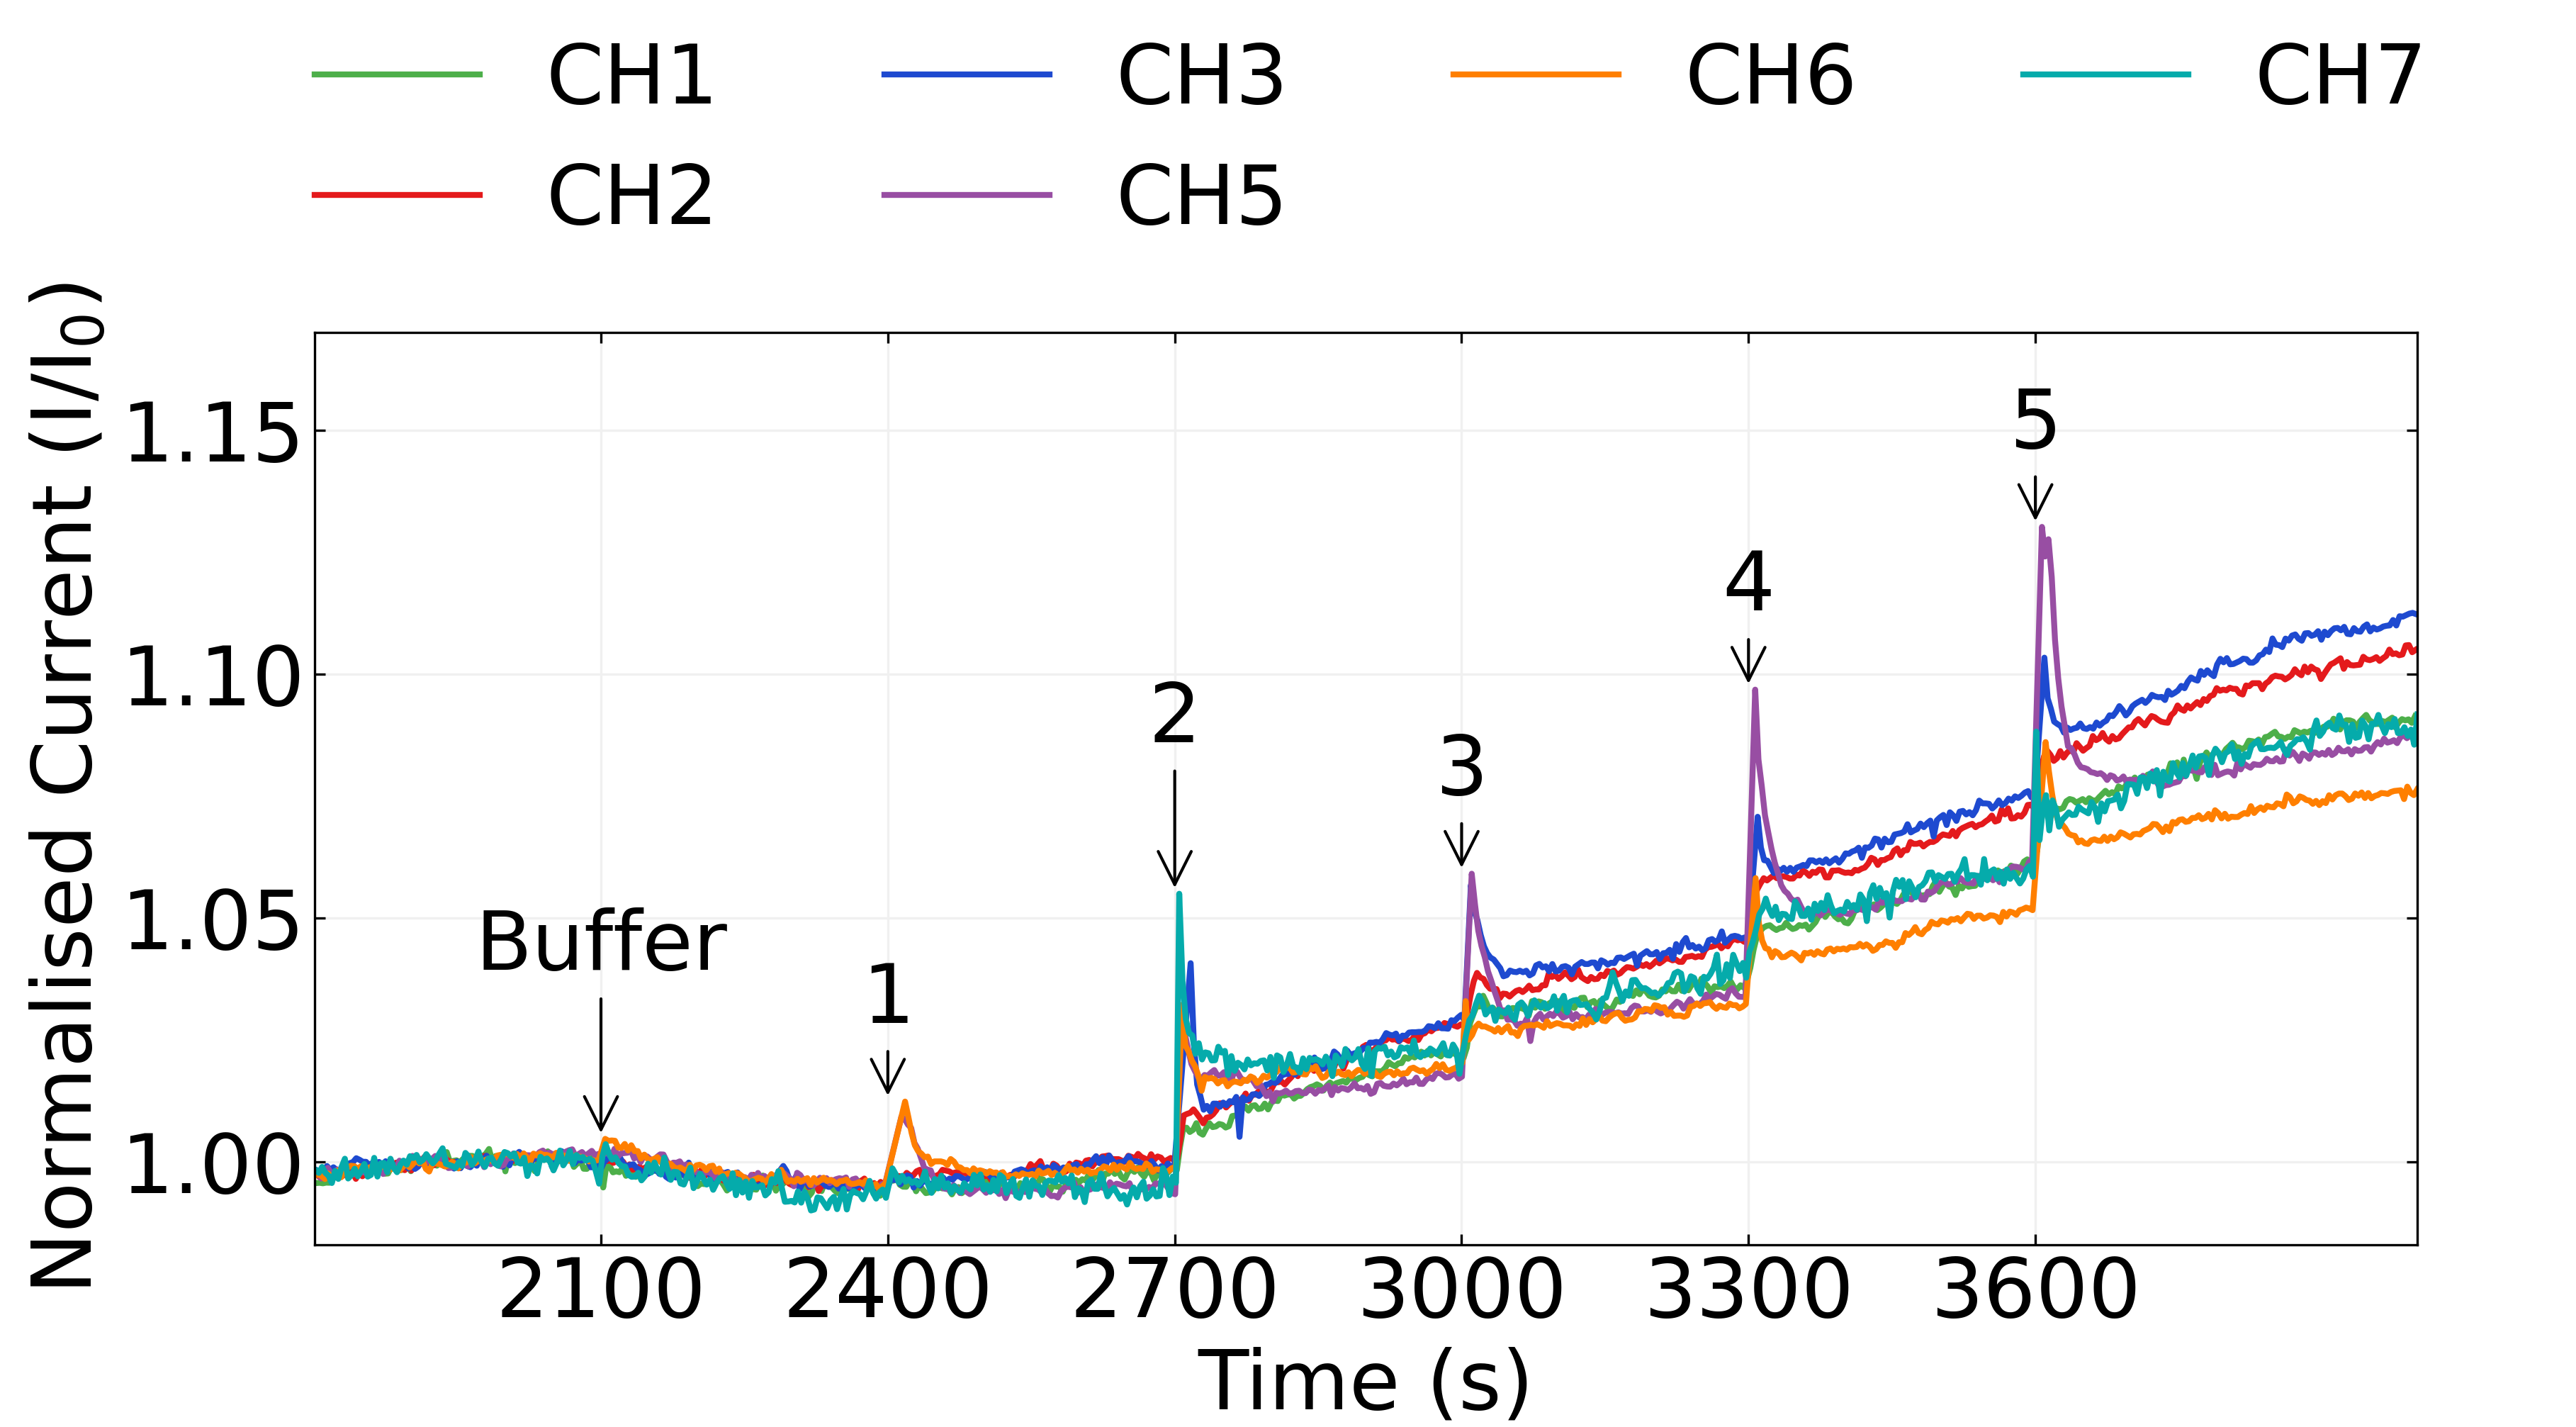
\includegraphics{figures/ch6/NTQ31C1_pristine_saltconc_sample_230324_detrend_trunc_arrows_normalised.png}

}

}

\subcaption{\label{fig-salt-conc-detrend}}
\end{minipage}%
\newline
\begin{minipage}[t]{0.50\linewidth}

{\centering 

\raisebox{-\height}{

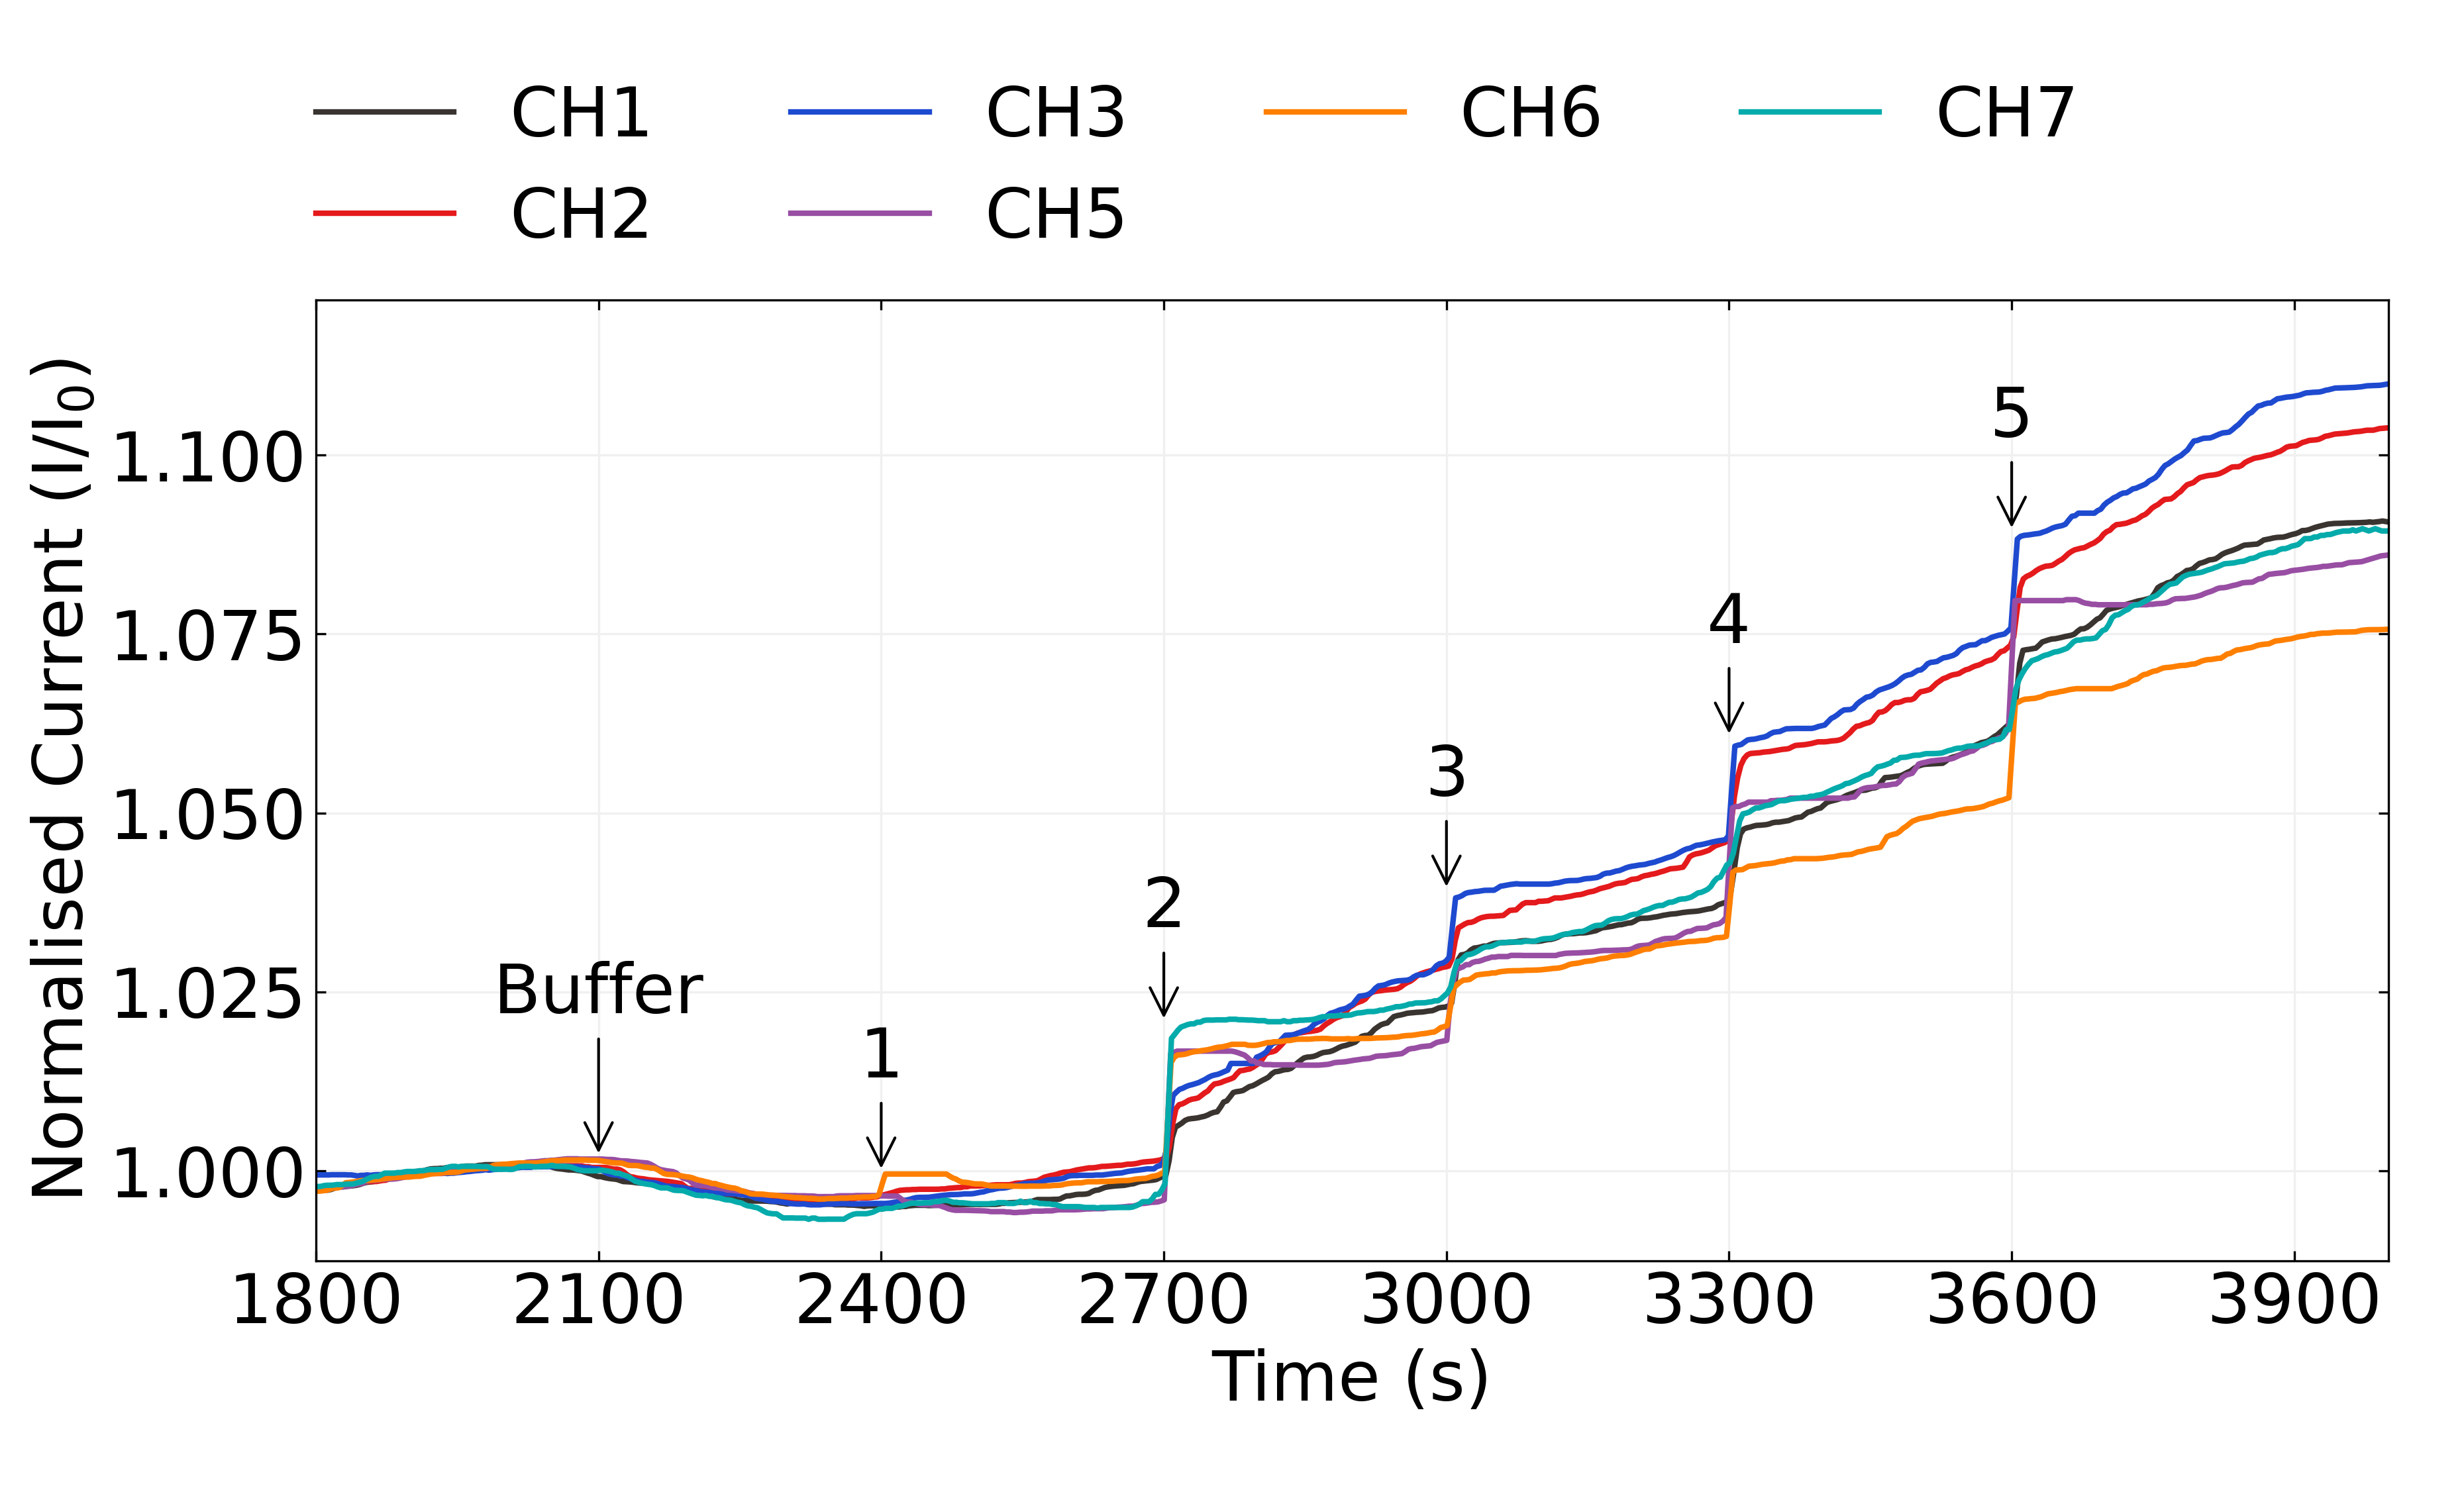
\includegraphics{figures/ch6/NTQ31C1_pristine_saltconc_sample_230324_filtered_detrend_trunc_arrows_normalised_(2).png}

}

}

\subcaption{\label{fig-salt-conc-detrend-filter}}
\end{minipage}%
%
\begin{minipage}[t]{0.50\linewidth}

{\centering 

\raisebox{-\height}{

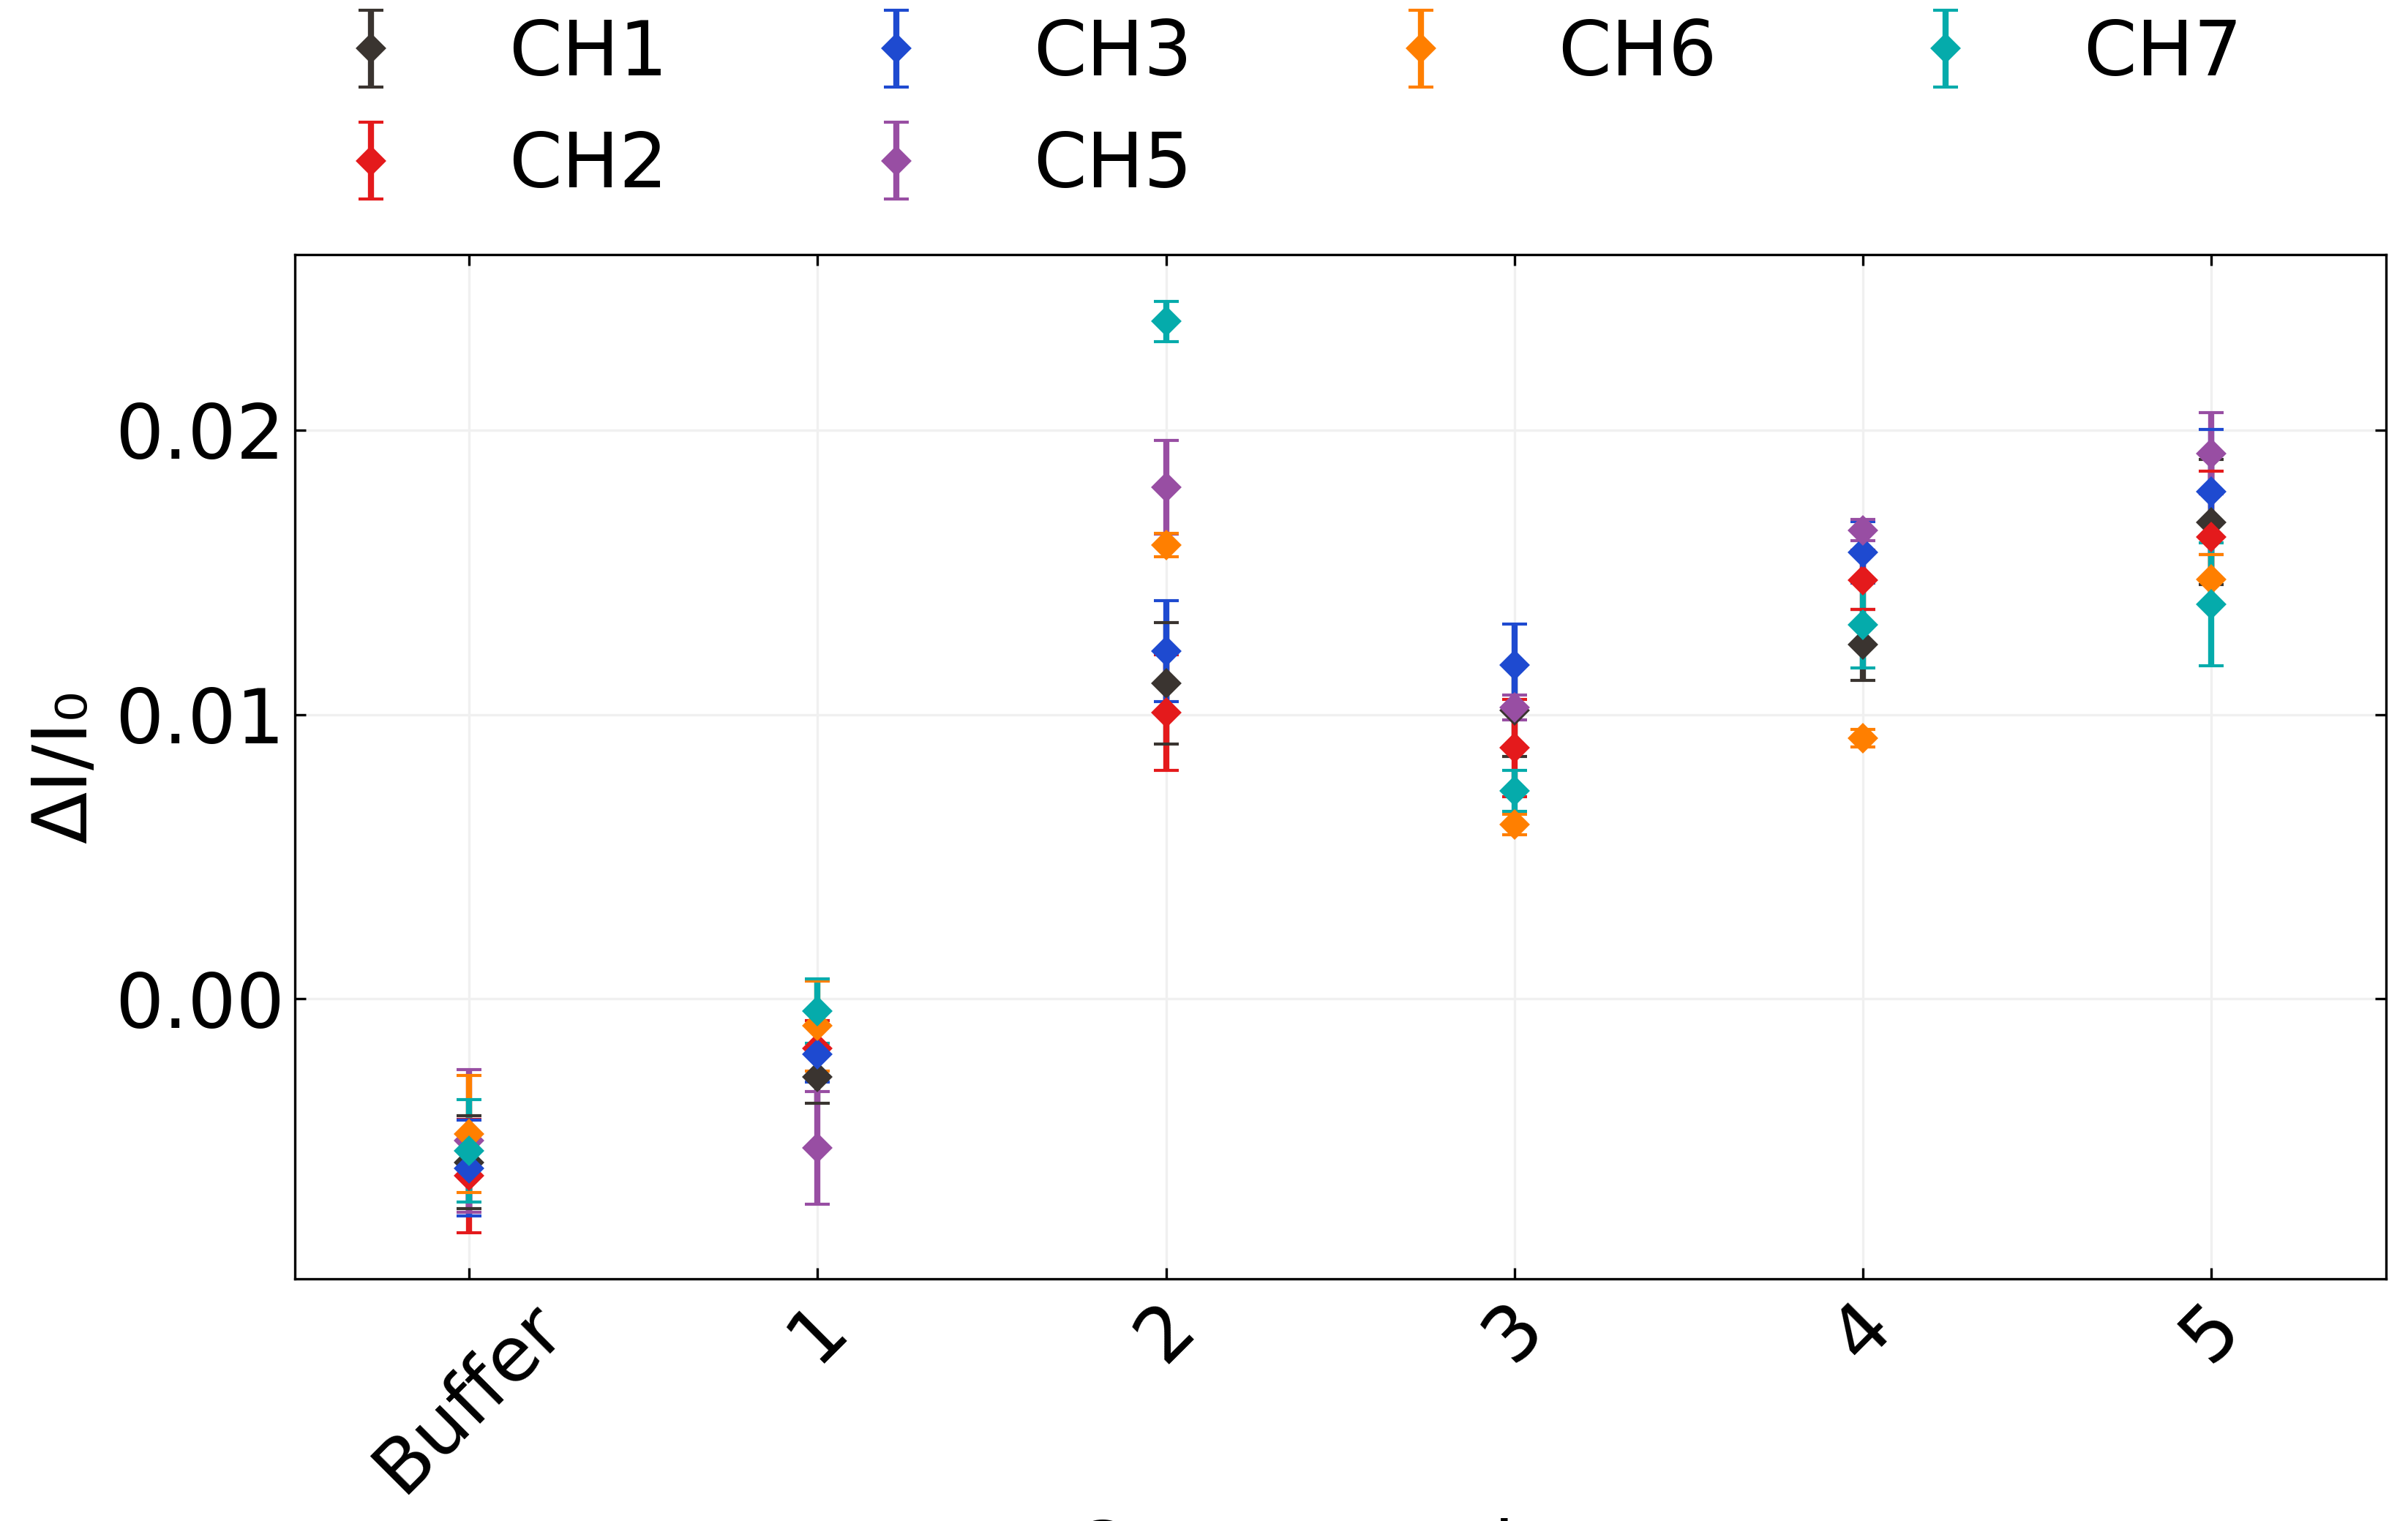
\includegraphics{figures/ch6/NTQ31C1_mean_simple_difference_before_and_after_step_filtered_concentrations.png}

}

}

\subcaption{\label{fig-salt-conc-signal}}
\end{minipage}%
\newline
\begin{minipage}[t]{0.25\linewidth}

{\centering 

~

}

\end{minipage}%
%
\begin{minipage}[t]{0.50\linewidth}

{\centering 

\raisebox{-\height}{

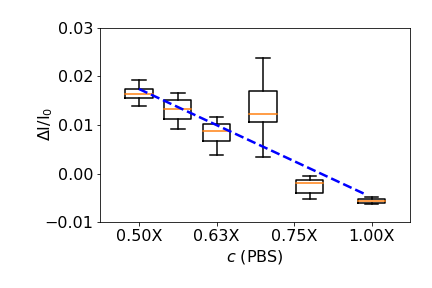
\includegraphics{figures/ch6/salt_conc_box_plot.png}

}

}

\subcaption{\label{fig-salt-conc-box-plot}}
\end{minipage}%
%
\begin{minipage}[t]{0.25\linewidth}

{\centering 

~

}

\end{minipage}%

\caption{\label{fig-salt-conc-sensing}Various visualisations of a
multiplexed salt concentration sensing series taken from a single
device. The source-drain voltage \(V_{ds}\) was 100 mV, and gate voltage
\(V_g\) was 0 V. In (a), the raw current measurements for each channel
are shown alongside gate current. The same measurements after despiking,
removal of baseline drift and normalisation to initial current are shown
in (b), (c) shows the data in (b) after being processed with a moving
median filter, and (d) shows the signal changes in (c). The signal data
in (d) is shown in box plot format in (e) alongside a fit to the median
change in signal for each addition. The R squared value for the fit was
0.86.}

\end{figure}

Figure~\ref{fig-salt-conc-no-norm} shows a multiplexed salt
concentration sensing series from the channels of a single
AZ\(^\circledR\) 1518 encapsulated device, measured with the NI-PXIe.
The gate voltage used was 0 V, which meant current measurements were
well above the magnitude of the subthreshold device current. Gate
current measurements did not exceed 1 nA for the SU8 encapsulated
devices, and did not exceed 10 nA for the AZ\(^\circledR\) 1518 devices.
At each of the deionised water addition times, the current traces for at
least two out of six channels showed a sharp, transient increase in
current followed by a return to an increased baseline. It is well
established that changing the salt concentration of the liquid gate has
an electrostatic gating effect on the carbon nanotubes or graphene, and
changes the transfer characteristics of the channel. This shift in
transfer characteristic leads to a real-time signal response to each
addition \autocite{Heller2009,Heller2010,Kireev2017}.

Using the data in Table~\ref{tbl-linear-fits}, the linear term
approximating baseline drift (\(c_1t\)) for each channel can be
subtracted from the data in Figure~\ref{fig-salt-conc-no-norm} to
account for the downward drift. The mean current level just before 1800
s then becomes roughly constant. Next, each channel is normalised
relative to their initial mean current level \(I_{0}\). Artifacts
resulting from PXIe-2737 module lag, single datapoints which fall well
below the current level of the immediately preceding and succeeding
datapoints, are also removed. This `despike' process uses an
interquartile range filter, which is described in
Section~\ref{sec-python-analysis}. The resulting dataset is shown in
Figure~\ref{fig-salt-conc-detrend}. This figure shows that the
signal-to-noise ratio remains roughly similar across all channels of the
device. However, the behaviour of the initial transient increase with
each addition is highly variable across channels and between additions
for a single channel.

As measurement of the highly variable initial transient is not useful
for robust sensing purposes, a moving median filter was applied, with
the implementation of this filter discussed in
Section~\ref{sec-python-analysis}. The filtered data is shown in
Figure~\ref{fig-salt-conc-detrend-filter}. Noise and initial transients
are removed completely, while the clearly defined step to a new current
baseline is retained. Using the realtime data in
Figure~\ref{fig-salt-conc-detrend-filter}, a plot of signal against
addition can be created using the method described in
Section~\ref{sec-python-analysis}, shown in
Figure~\ref{fig-salt-conc-signal}. This presentation of the data allows
us to see the increase at each step relative to \(I_{0}\).

Intriguingly, even though the largest change in PBS concentration
occurred at the first deionised water addition (see
Table~\ref{tbl-salt-conc-series}), there was very little signal change
across all channels, while a relatively large change occurred at the
second addition. The logarithm of final salt concentration has
previously been shown to be proportional to conductance change in the
linear on-regime \autocite{Heller2010}.
Figure~\ref{fig-salt-conc-box-plot} shows the signal change presented in
terms of this logarithmic relationship. The median values of the first
two additions do not line up well with the overall logarithmic trend;
insufficient mixing in the tightly enclosed PDMS well environment for
the first few additions may be responsible for this result. Subsequent
additions may improve mixing in the well, leading to the change in
concentration at the surface of the channel being more representative of
the overall concentration in the well.

\begin{figure}

\begin{minipage}[t]{0.50\linewidth}

{\centering 

\raisebox{-\height}{

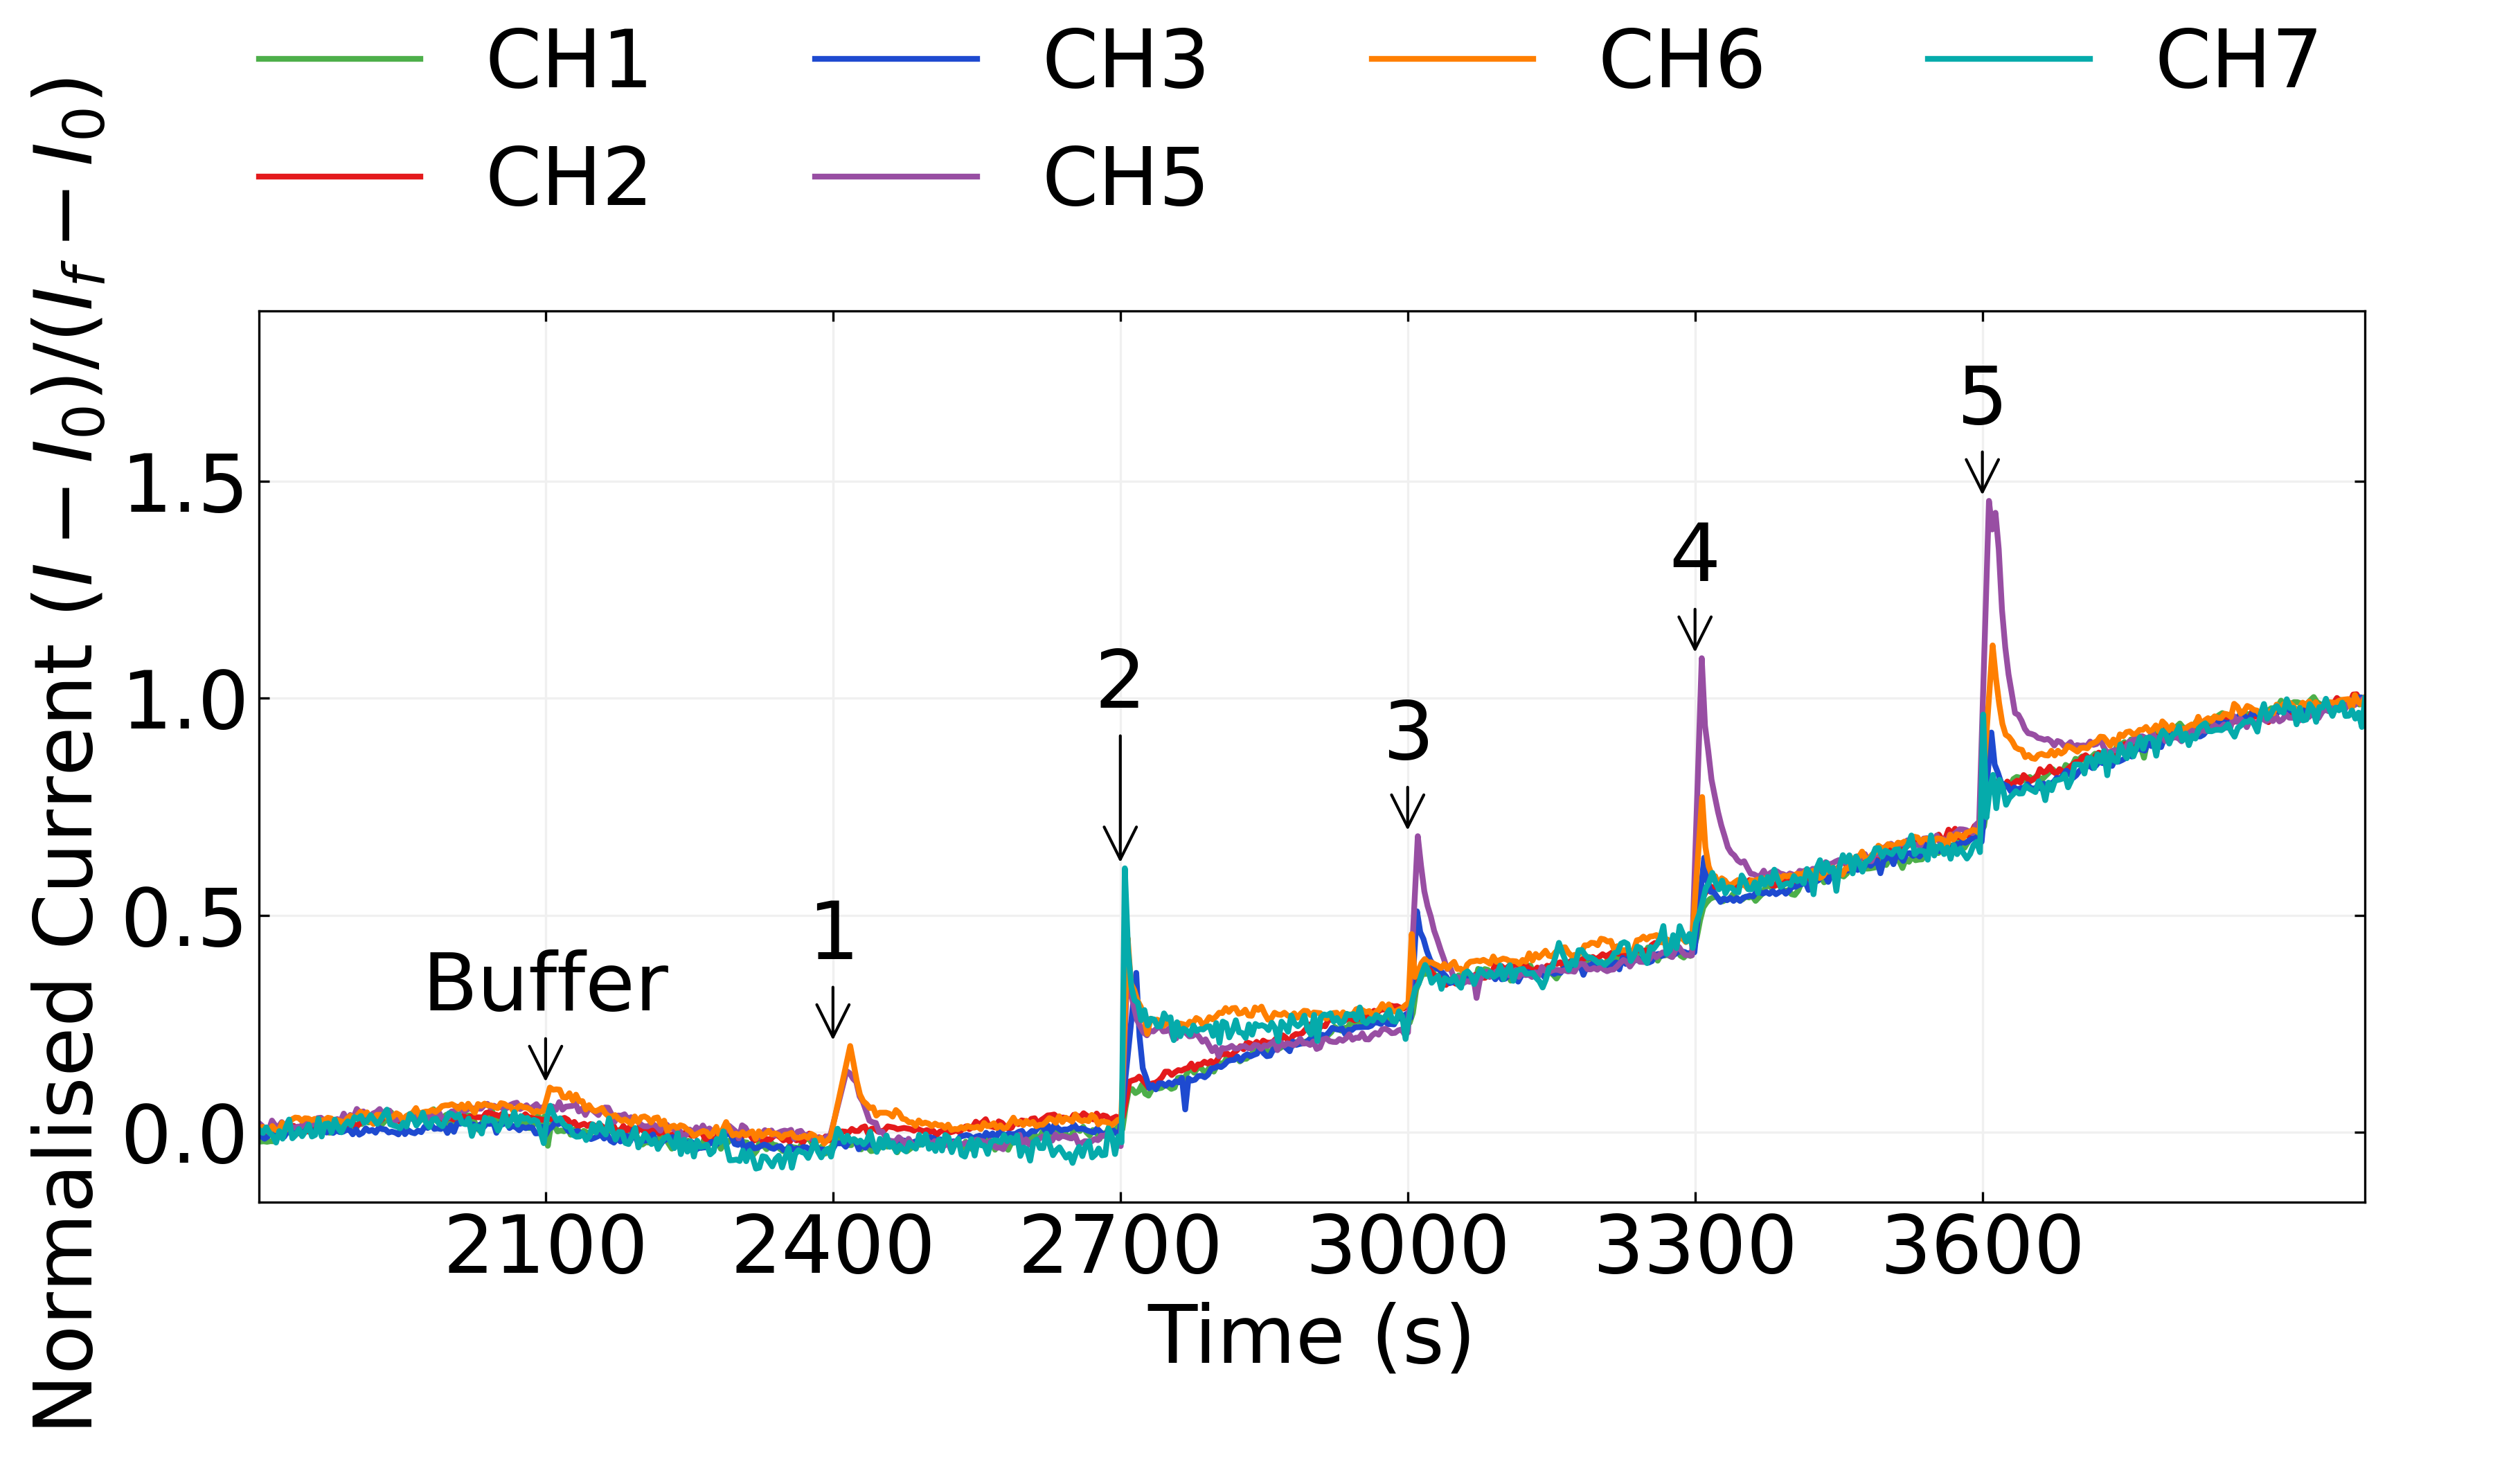
\includegraphics{figures/ch6/NTQ31C1_pristine_saltconc_sample_230324_detrend_trunc_arrows_normalised_2.png}

}

}

\subcaption{\label{fig-salt-conc-detrend-2}}
\end{minipage}%
%
\begin{minipage}[t]{0.50\linewidth}

{\centering 

\raisebox{-\height}{

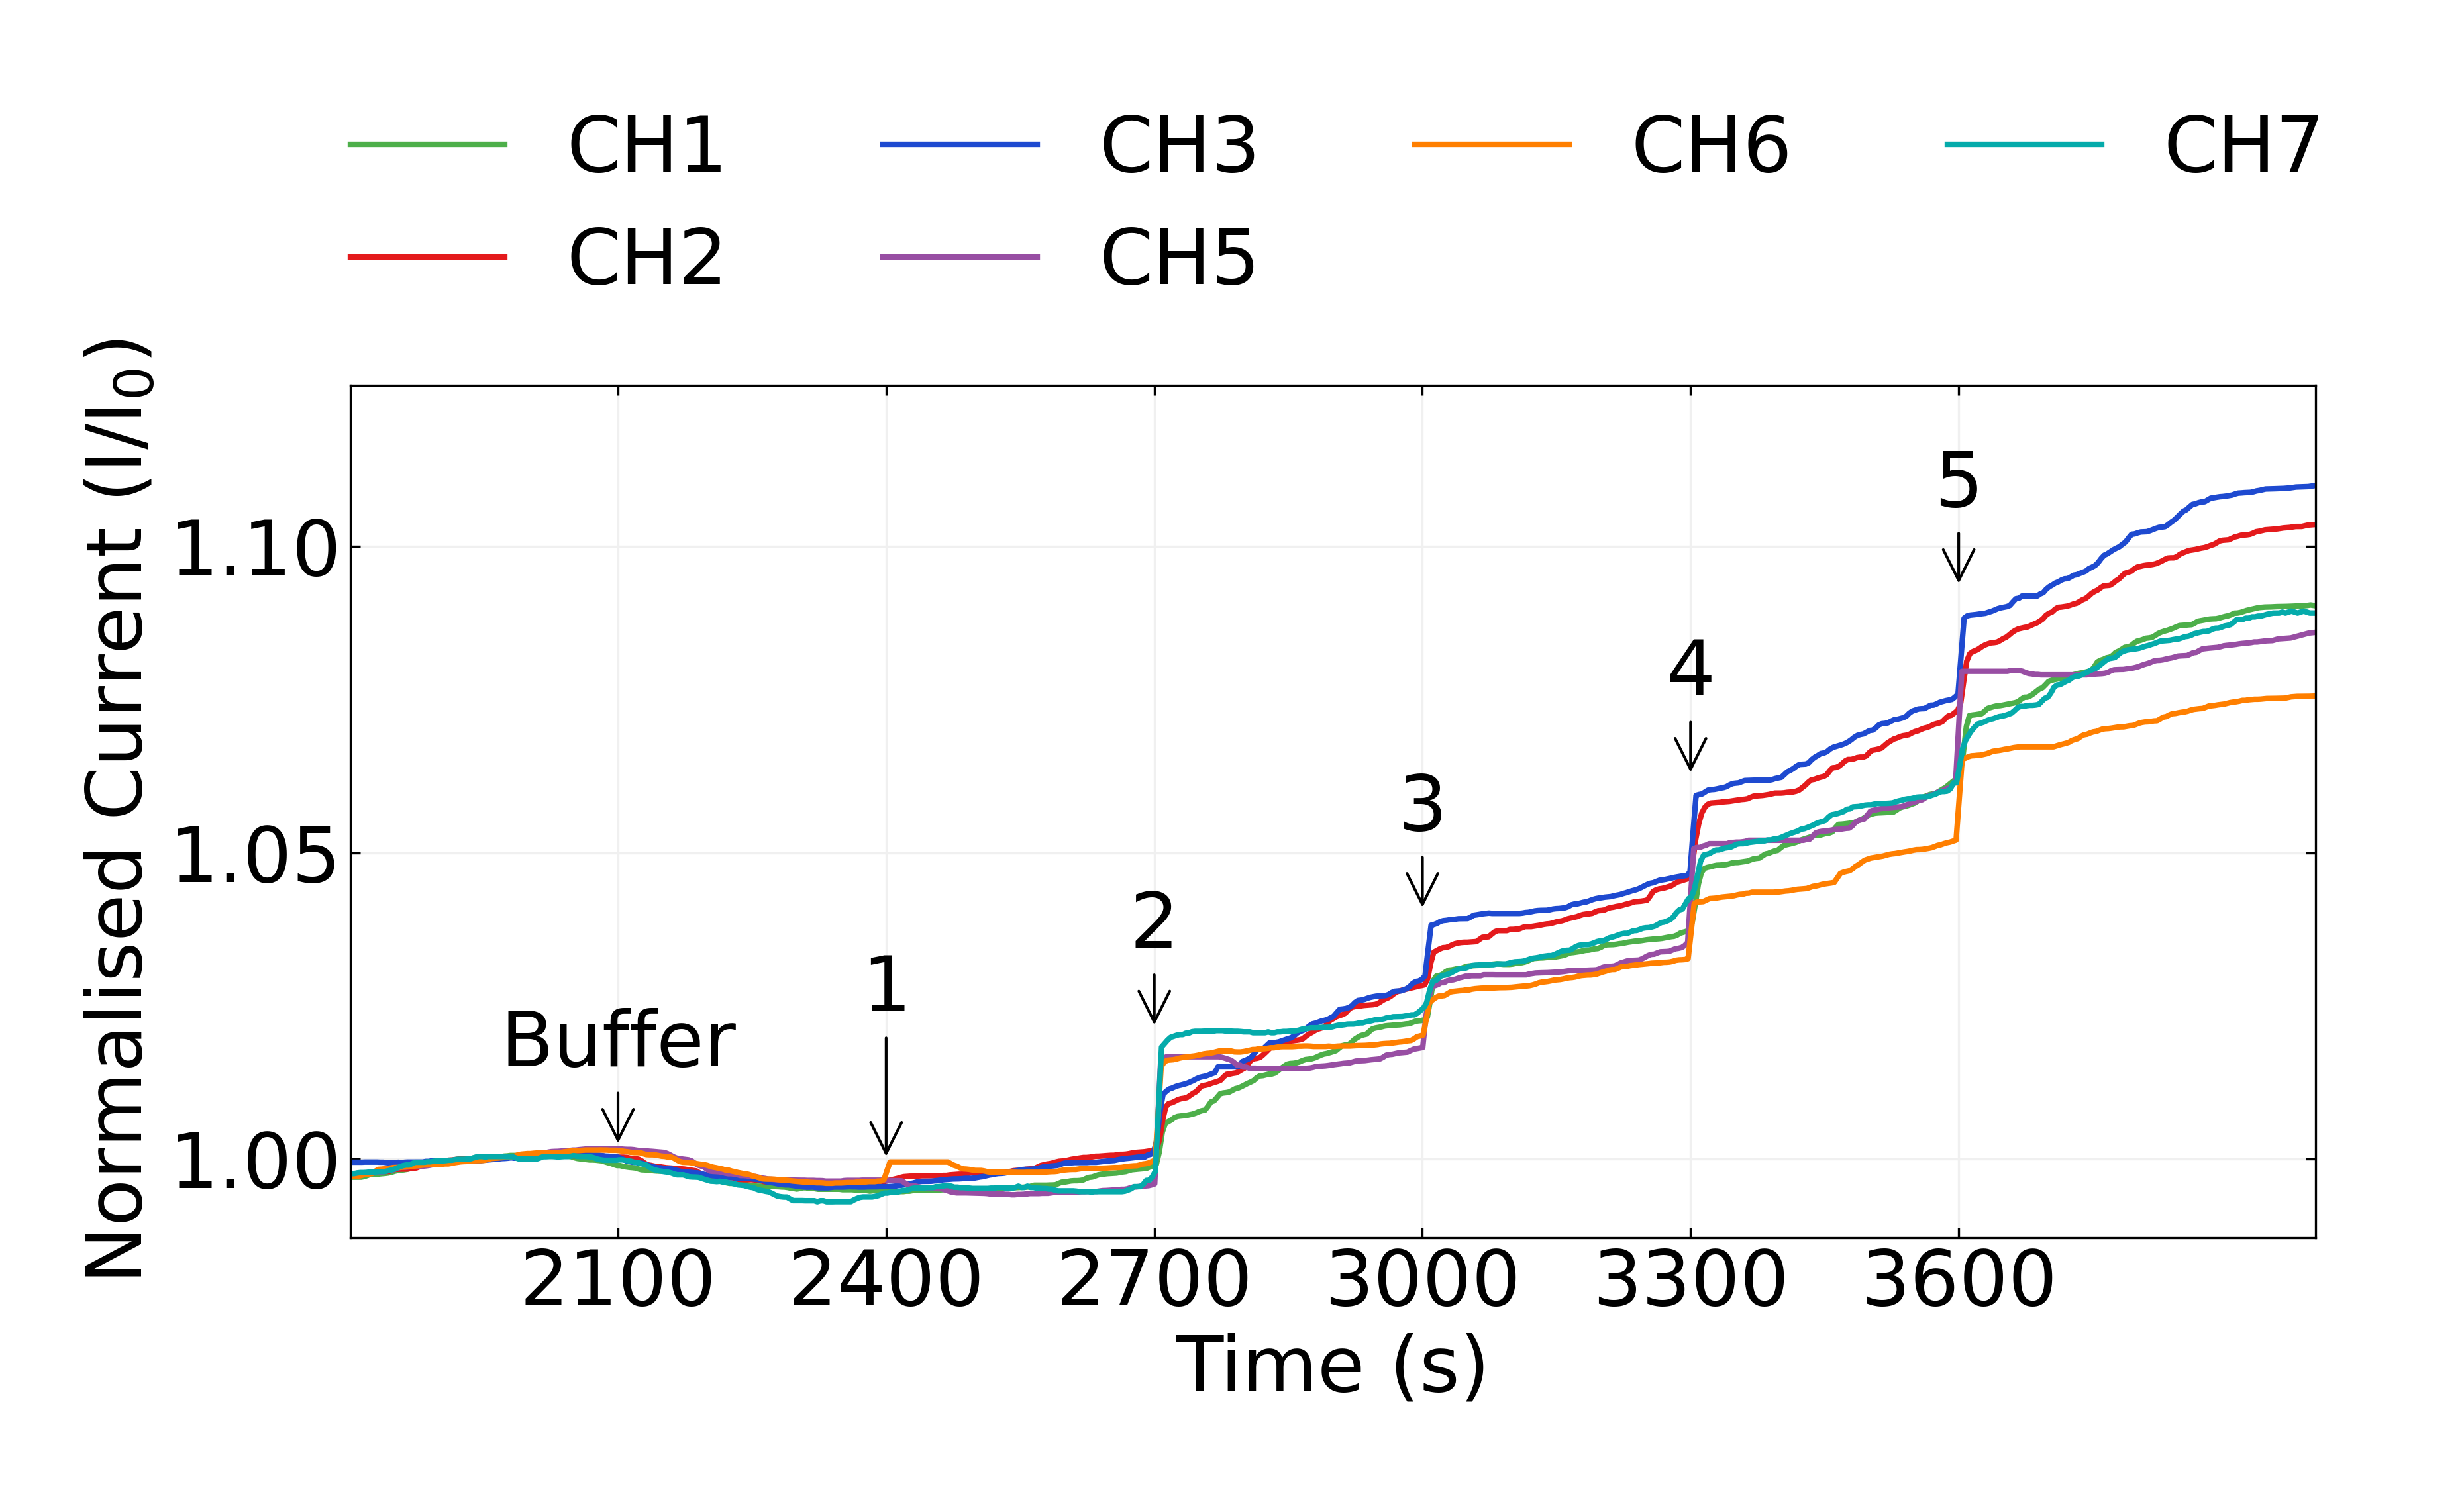
\includegraphics{figures/ch6/NTQ31C1_pristine_saltconc_sample_230324_filtered_detrend_trunc_arrows_normalised.png}

}

}

\subcaption{\label{fig-salt-conc-detrend-filter-2}}
\end{minipage}%
\newline
\begin{minipage}[t]{0.28\linewidth}

{\centering 

~

}

\end{minipage}%
%
\begin{minipage}[t]{0.45\linewidth}

{\centering 

\raisebox{-\height}{

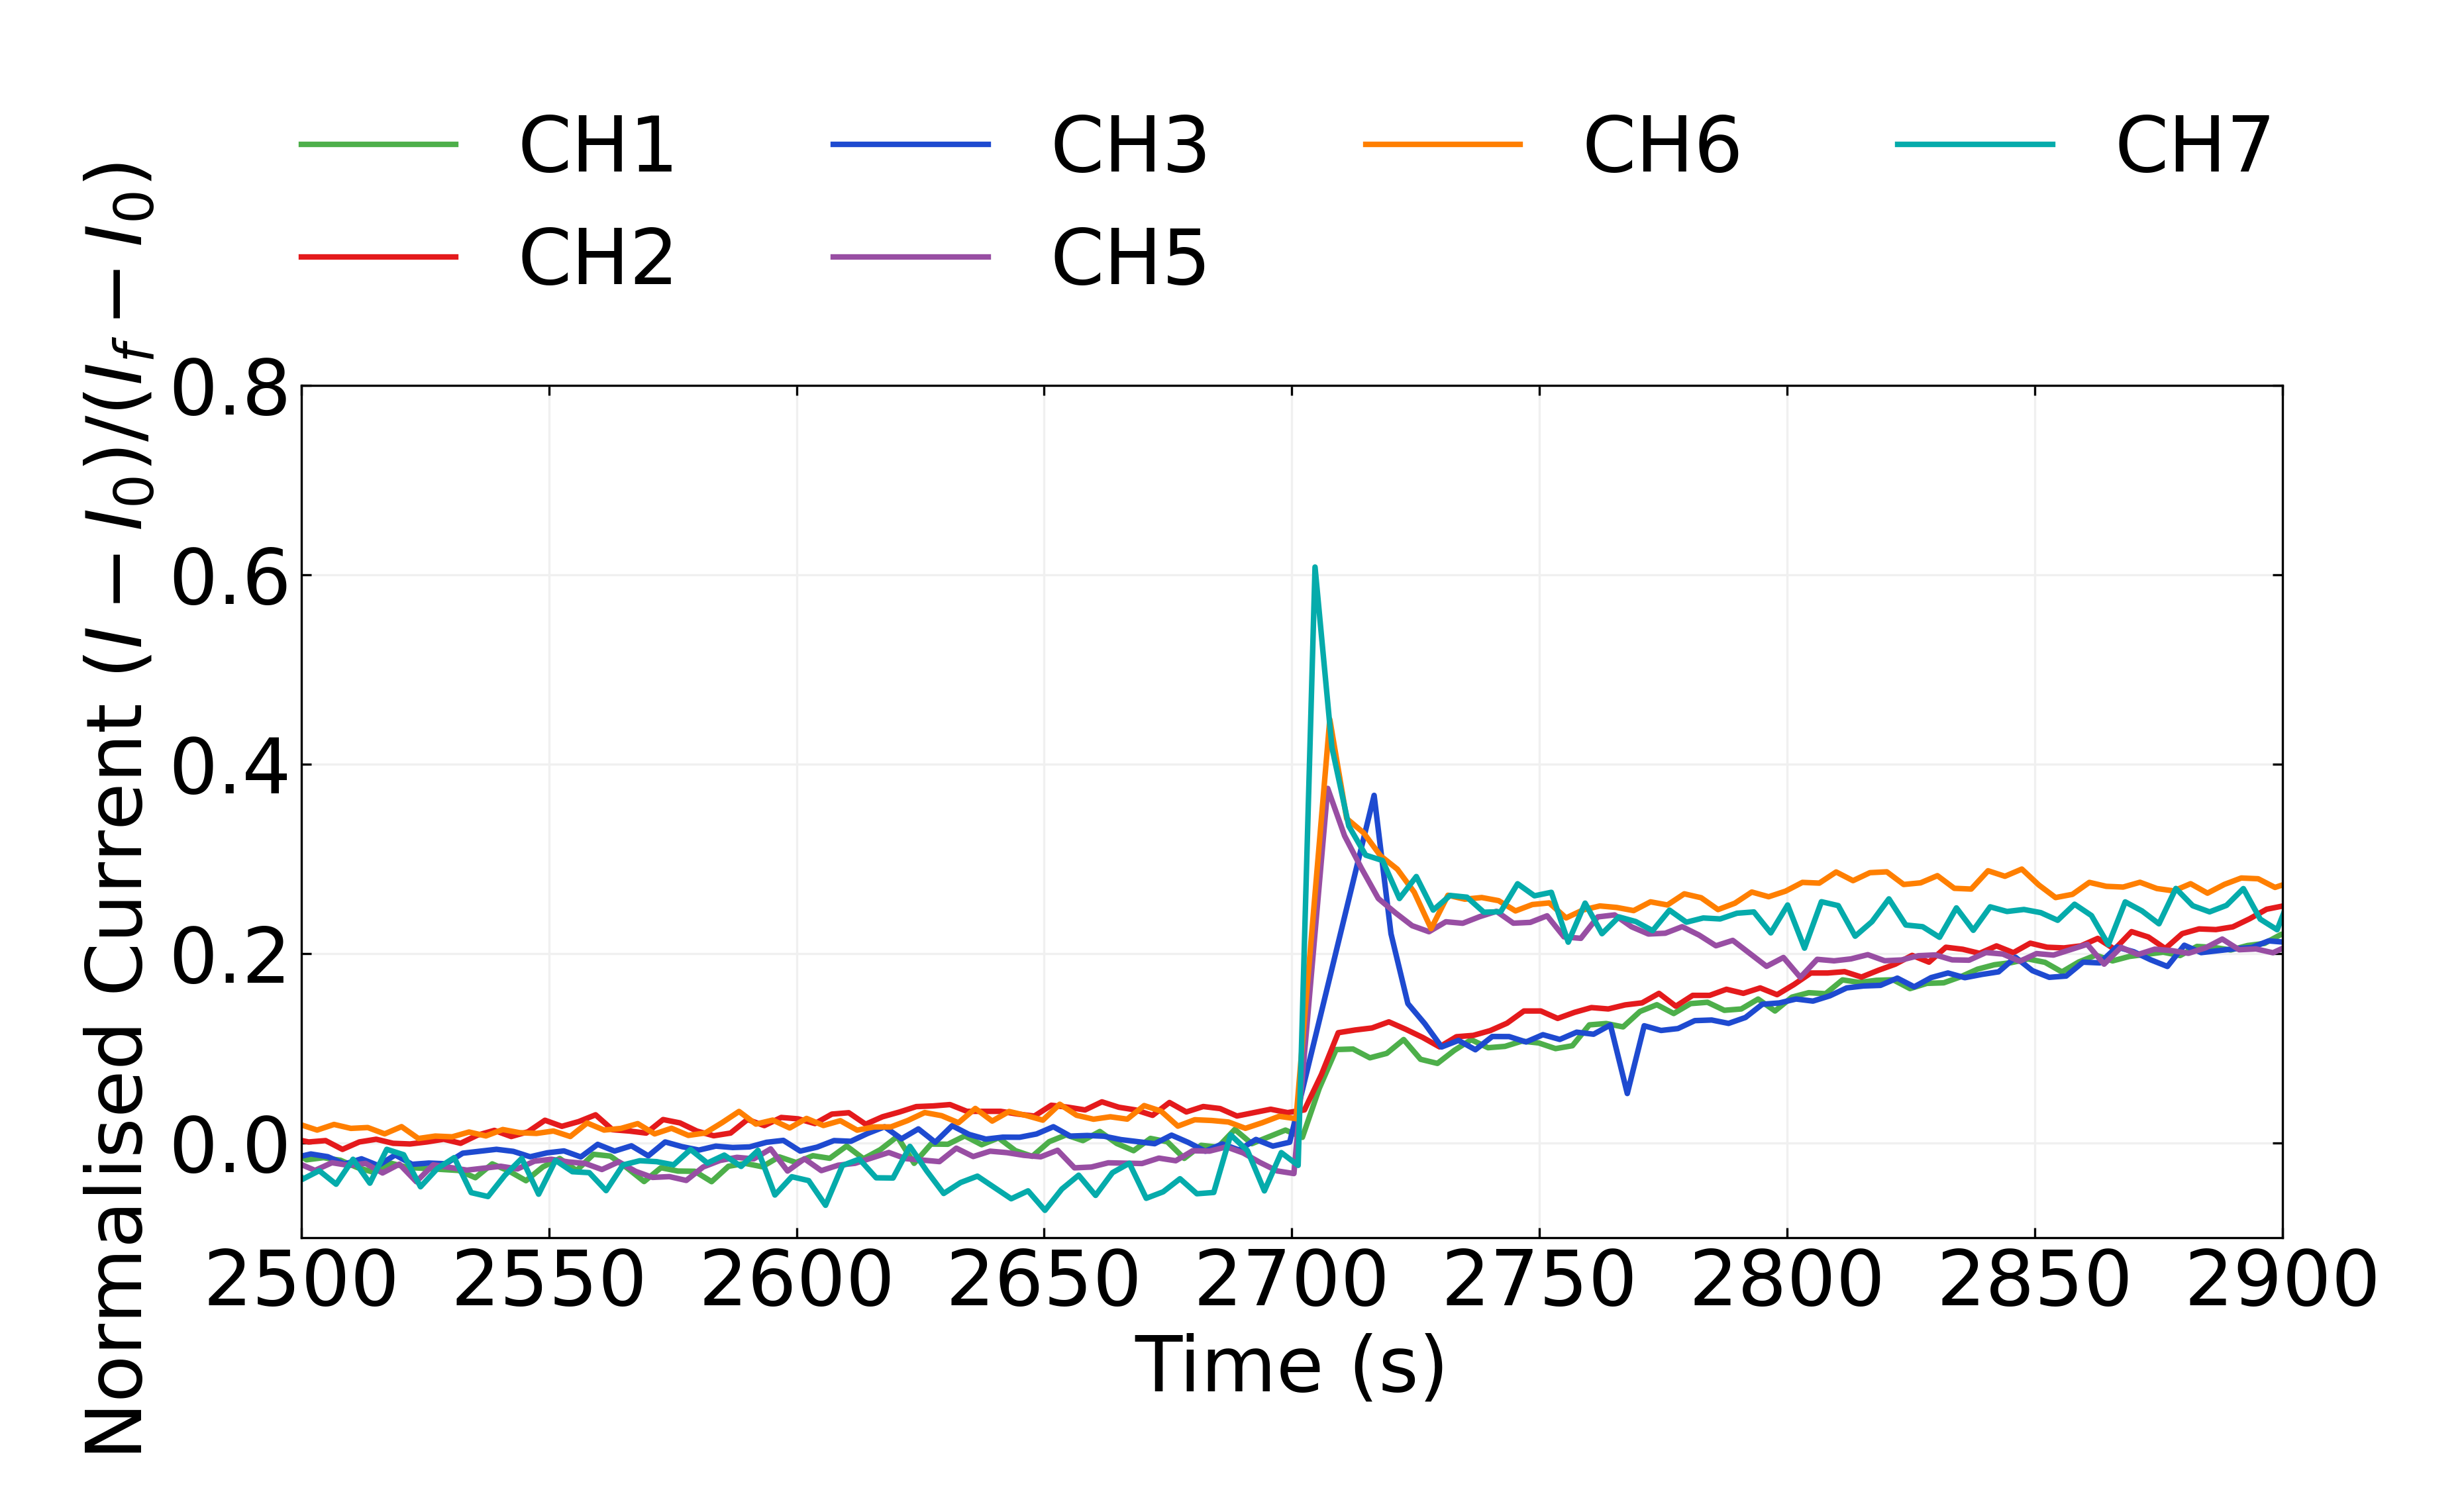
\includegraphics{figures/ch6/NTQ31C1_pristine_saltconc_sample_230324_single_step.png}

}

}

\subcaption{\label{fig-salt-conc-detrend-filter-single-step}}
\end{minipage}%
%
\begin{minipage}[t]{0.28\linewidth}

{\centering 

~

}

\end{minipage}%

\caption{\label{fig-salt-conc-sensing-2}The processed data shown in
Figure~\ref{fig-salt-conc-detrend} and
Figure~\ref{fig-salt-conc-detrend-filter} is normalised to \(I_{0}\),
but an alternative normalisation can more effectively filter out
remaining drift present. This normalisation presents data relative to
both \(I_{0}\) and the final current reading \(I_{f}\) using the formula
\((I - I_{0})/(I_{f} - I_{0})\). Using this normalisation, the data in
Figure~\ref{fig-salt-conc-detrend} and
Figure~\ref{fig-salt-conc-detrend-filter} can be displayed instead as
(a) and (b) respectively. (c) shows a magnified version of the step at
addition 2 in (a).}

\end{figure}

In Figure~\ref{fig-salt-conc-detrend} and
Figure~\ref{fig-salt-conc-detrend-filter}, from around the second
deionised water addition onwards, the drift behaviours of individual
channels begin to significantly diverge. This deviation from the
baseline drift subtracted from the raw data occurs either because the
linear fit is only a first-order approximation which weakens with time,
or because the additions themselves affect the drift behaviour.
Displaying the data as discrete signal changes, as in
Figure~\ref{fig-salt-conc-signal}, is one way of excluding these
deviations (see Section~\ref{sec-python-analysis}). An alternative way
of presenting the signal changes, by normalising relative to both
\(I_{0}\) and the final current reading with the formula
\((I - I_{0})/(I_{f} - I_{0})\), is shown in
Figure~\ref{fig-salt-conc-sensing-2}. This approach is useful for
filtering out remaining unaccounted-for drift behaviour in order to
compare the short-term transient responses to additions across the
device channels. Furthermore, it lets us better understand how the
short-term transient responses affect the longer-term step responses
discussed earlier.

Figure~\ref{fig-salt-conc-detrend-2} and
Figure~\ref{fig-salt-conc-detrend-filter-single-step} show that the
transient responses to DI water additions vary significantly across the
surface of the device. For example,
Figure~\ref{fig-salt-conc-detrend-filter-single-step} shows that in
response to the second DI water addition, channel 7 gives a large
initial transient response about twice the size of the step increase
between 2600 and 2800 s. Meanwhile, channels 1 and 2 show no transient
response above the step increase.
Figure~\ref{fig-salt-conc-detrend-filter-single-step} indicates
transient size is based on location across the device, with neighbouring
channels showing the most similar behaviour. This spatially-dependent
behaviour may indicate transient responses are determined by the
location of the channel relative to either the location of water
additions or the slightly-variable location of the liquid gate. Larger
and longer-lasting transient responses are not entirely removed by the
moving median filter, as shown by comparing
Figure~\ref{fig-salt-conc-detrend-2} to
Figure~\ref{fig-salt-conc-detrend-filter}, and so careful placement of
additions is important when sensing to minimise this effect. However,
even the longest-lasting transients appear to decay to zero within about
200 s, demonstrating that a 200 s spacing between additions at minimum
is necessary for reliable real-time liquid-gated sensing using this
setup.

\hypertarget{signal-to-noise-ratio}{%
\subsubsection*{Signal-to-Noise Ratio}\label{signal-to-noise-ratio}}
\addcontentsline{toc}{subsubsection}{Signal-to-Noise Ratio}

\begin{figure}

\begin{minipage}[t]{0.45\linewidth}

{\centering 

\raisebox{-\height}{

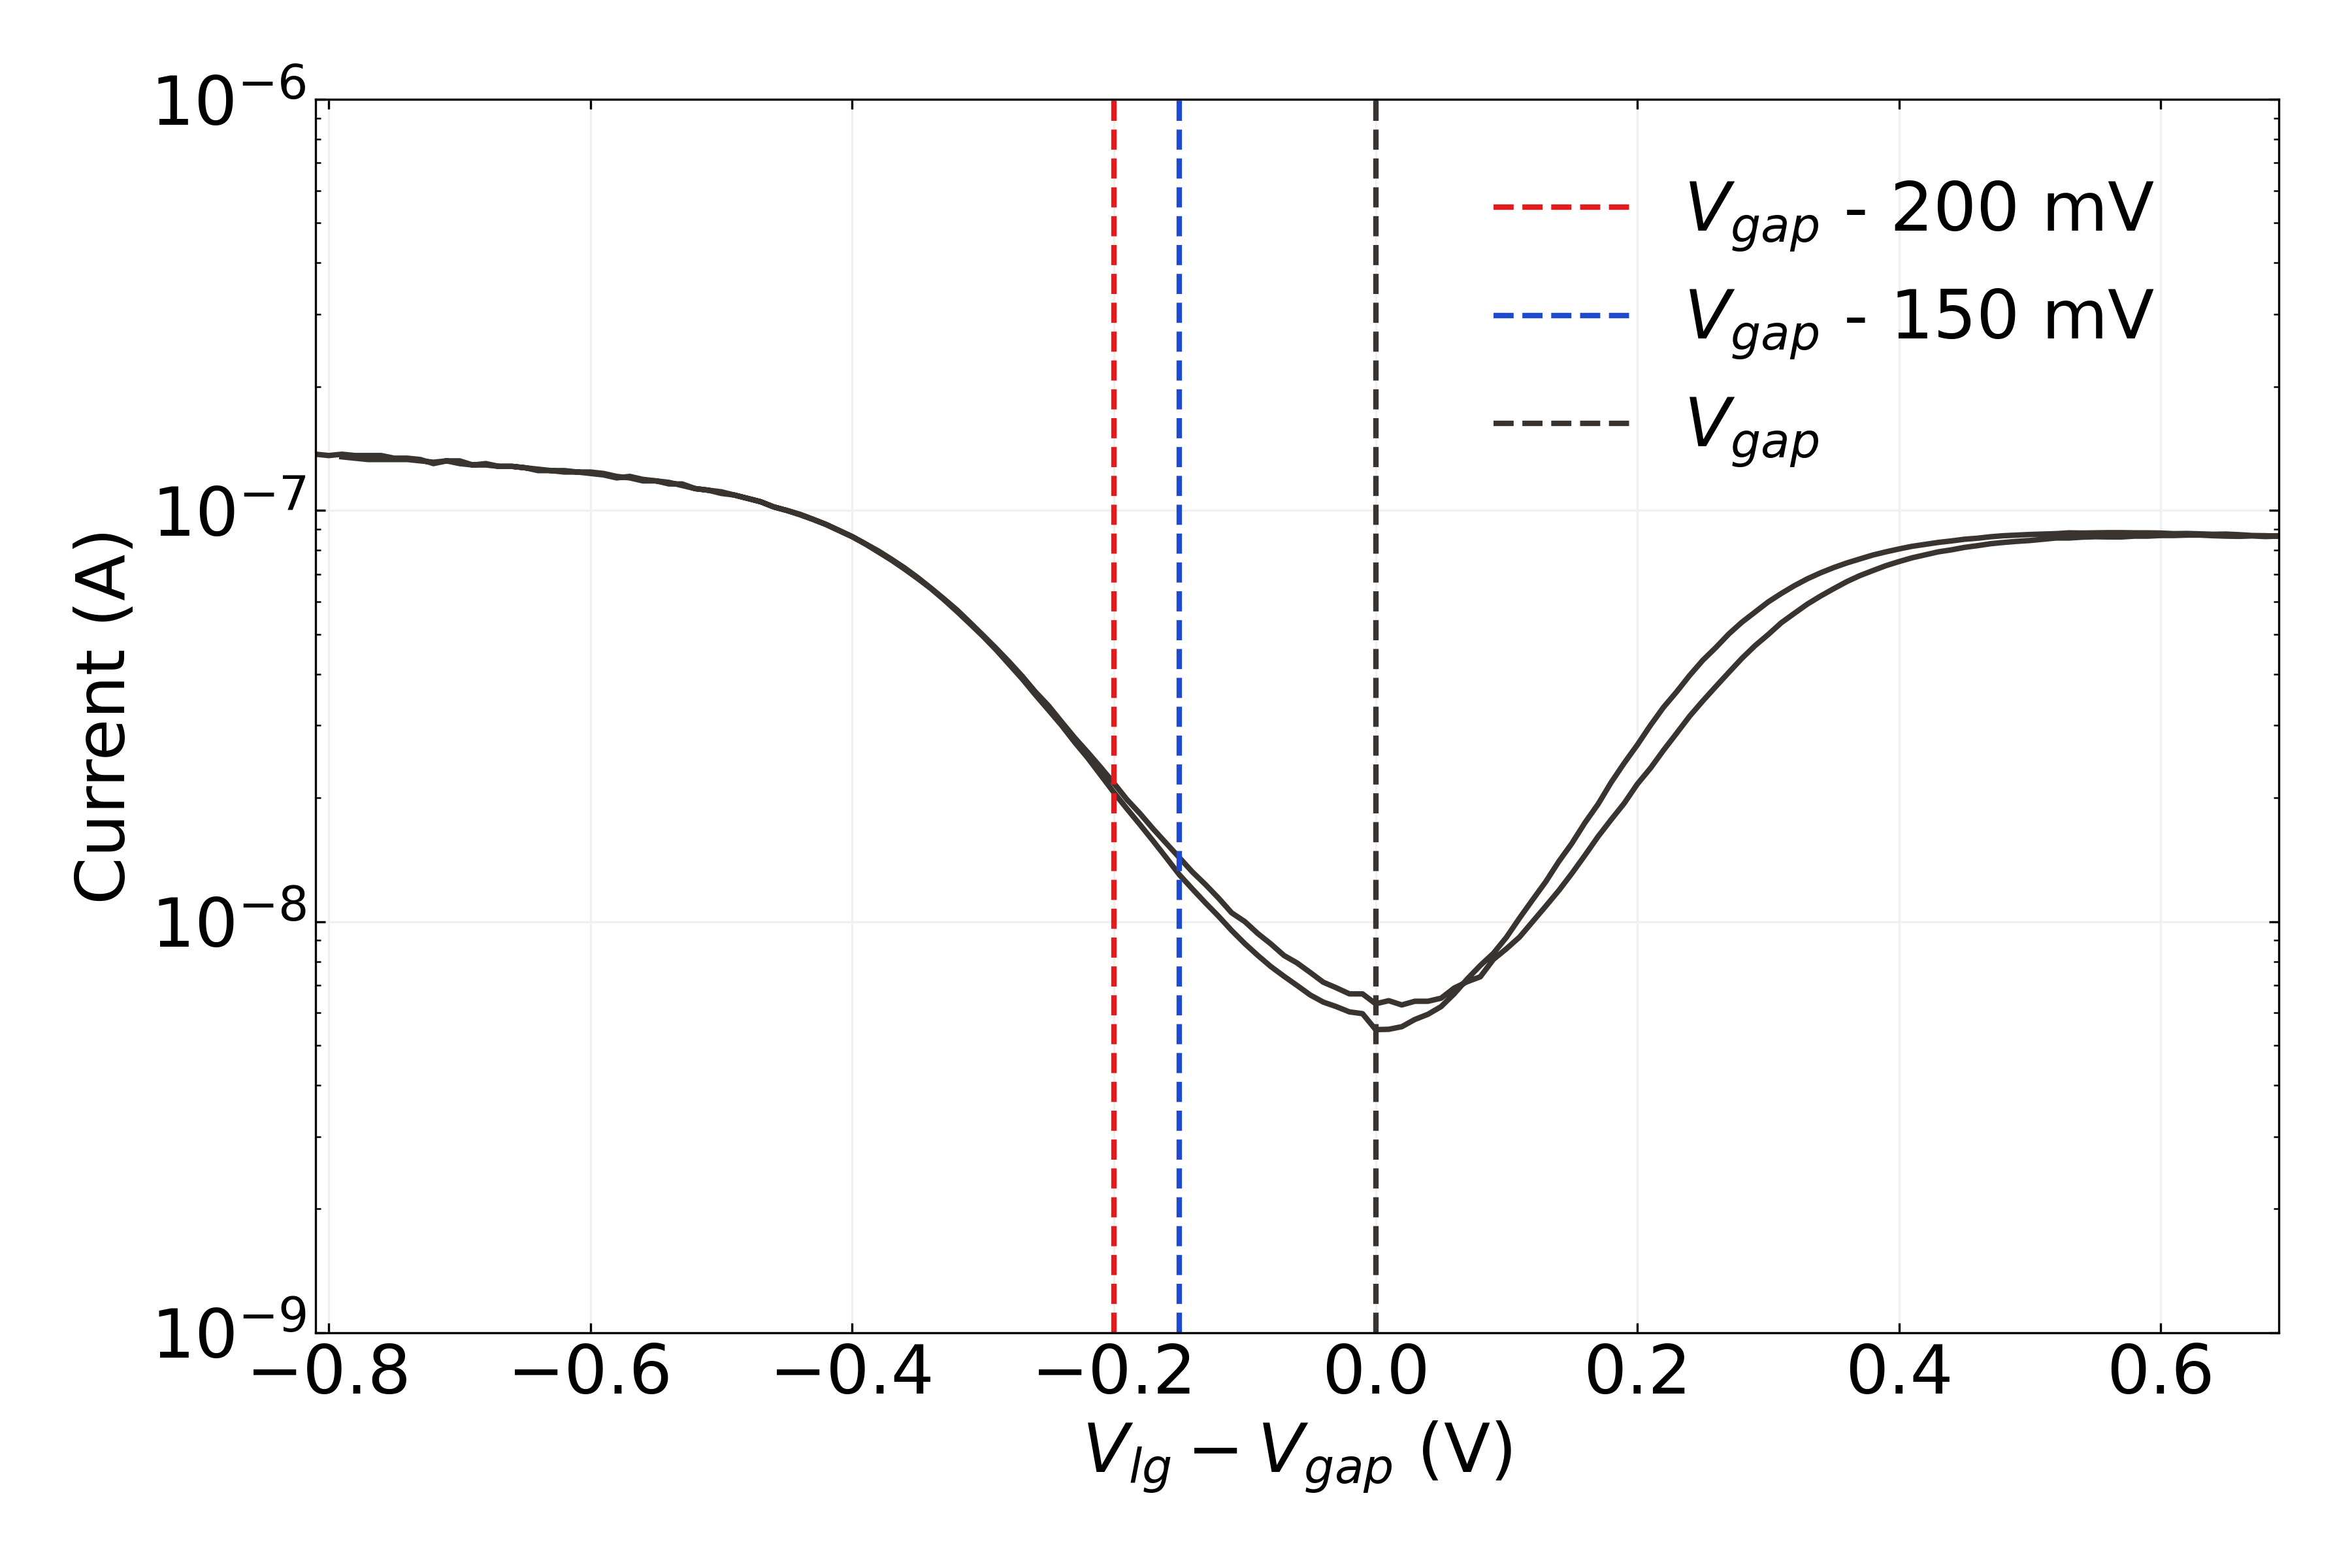
\includegraphics{figures/ch6/Q2C10ch8custom.png}

}

}

\subcaption{\label{fig-transfer-sweep-2}}
\end{minipage}%
%
\begin{minipage}[t]{0.05\linewidth}

{\centering 

~

}

\end{minipage}%
%
\begin{minipage}[t]{0.50\linewidth}

{\centering 

\raisebox{-\height}{

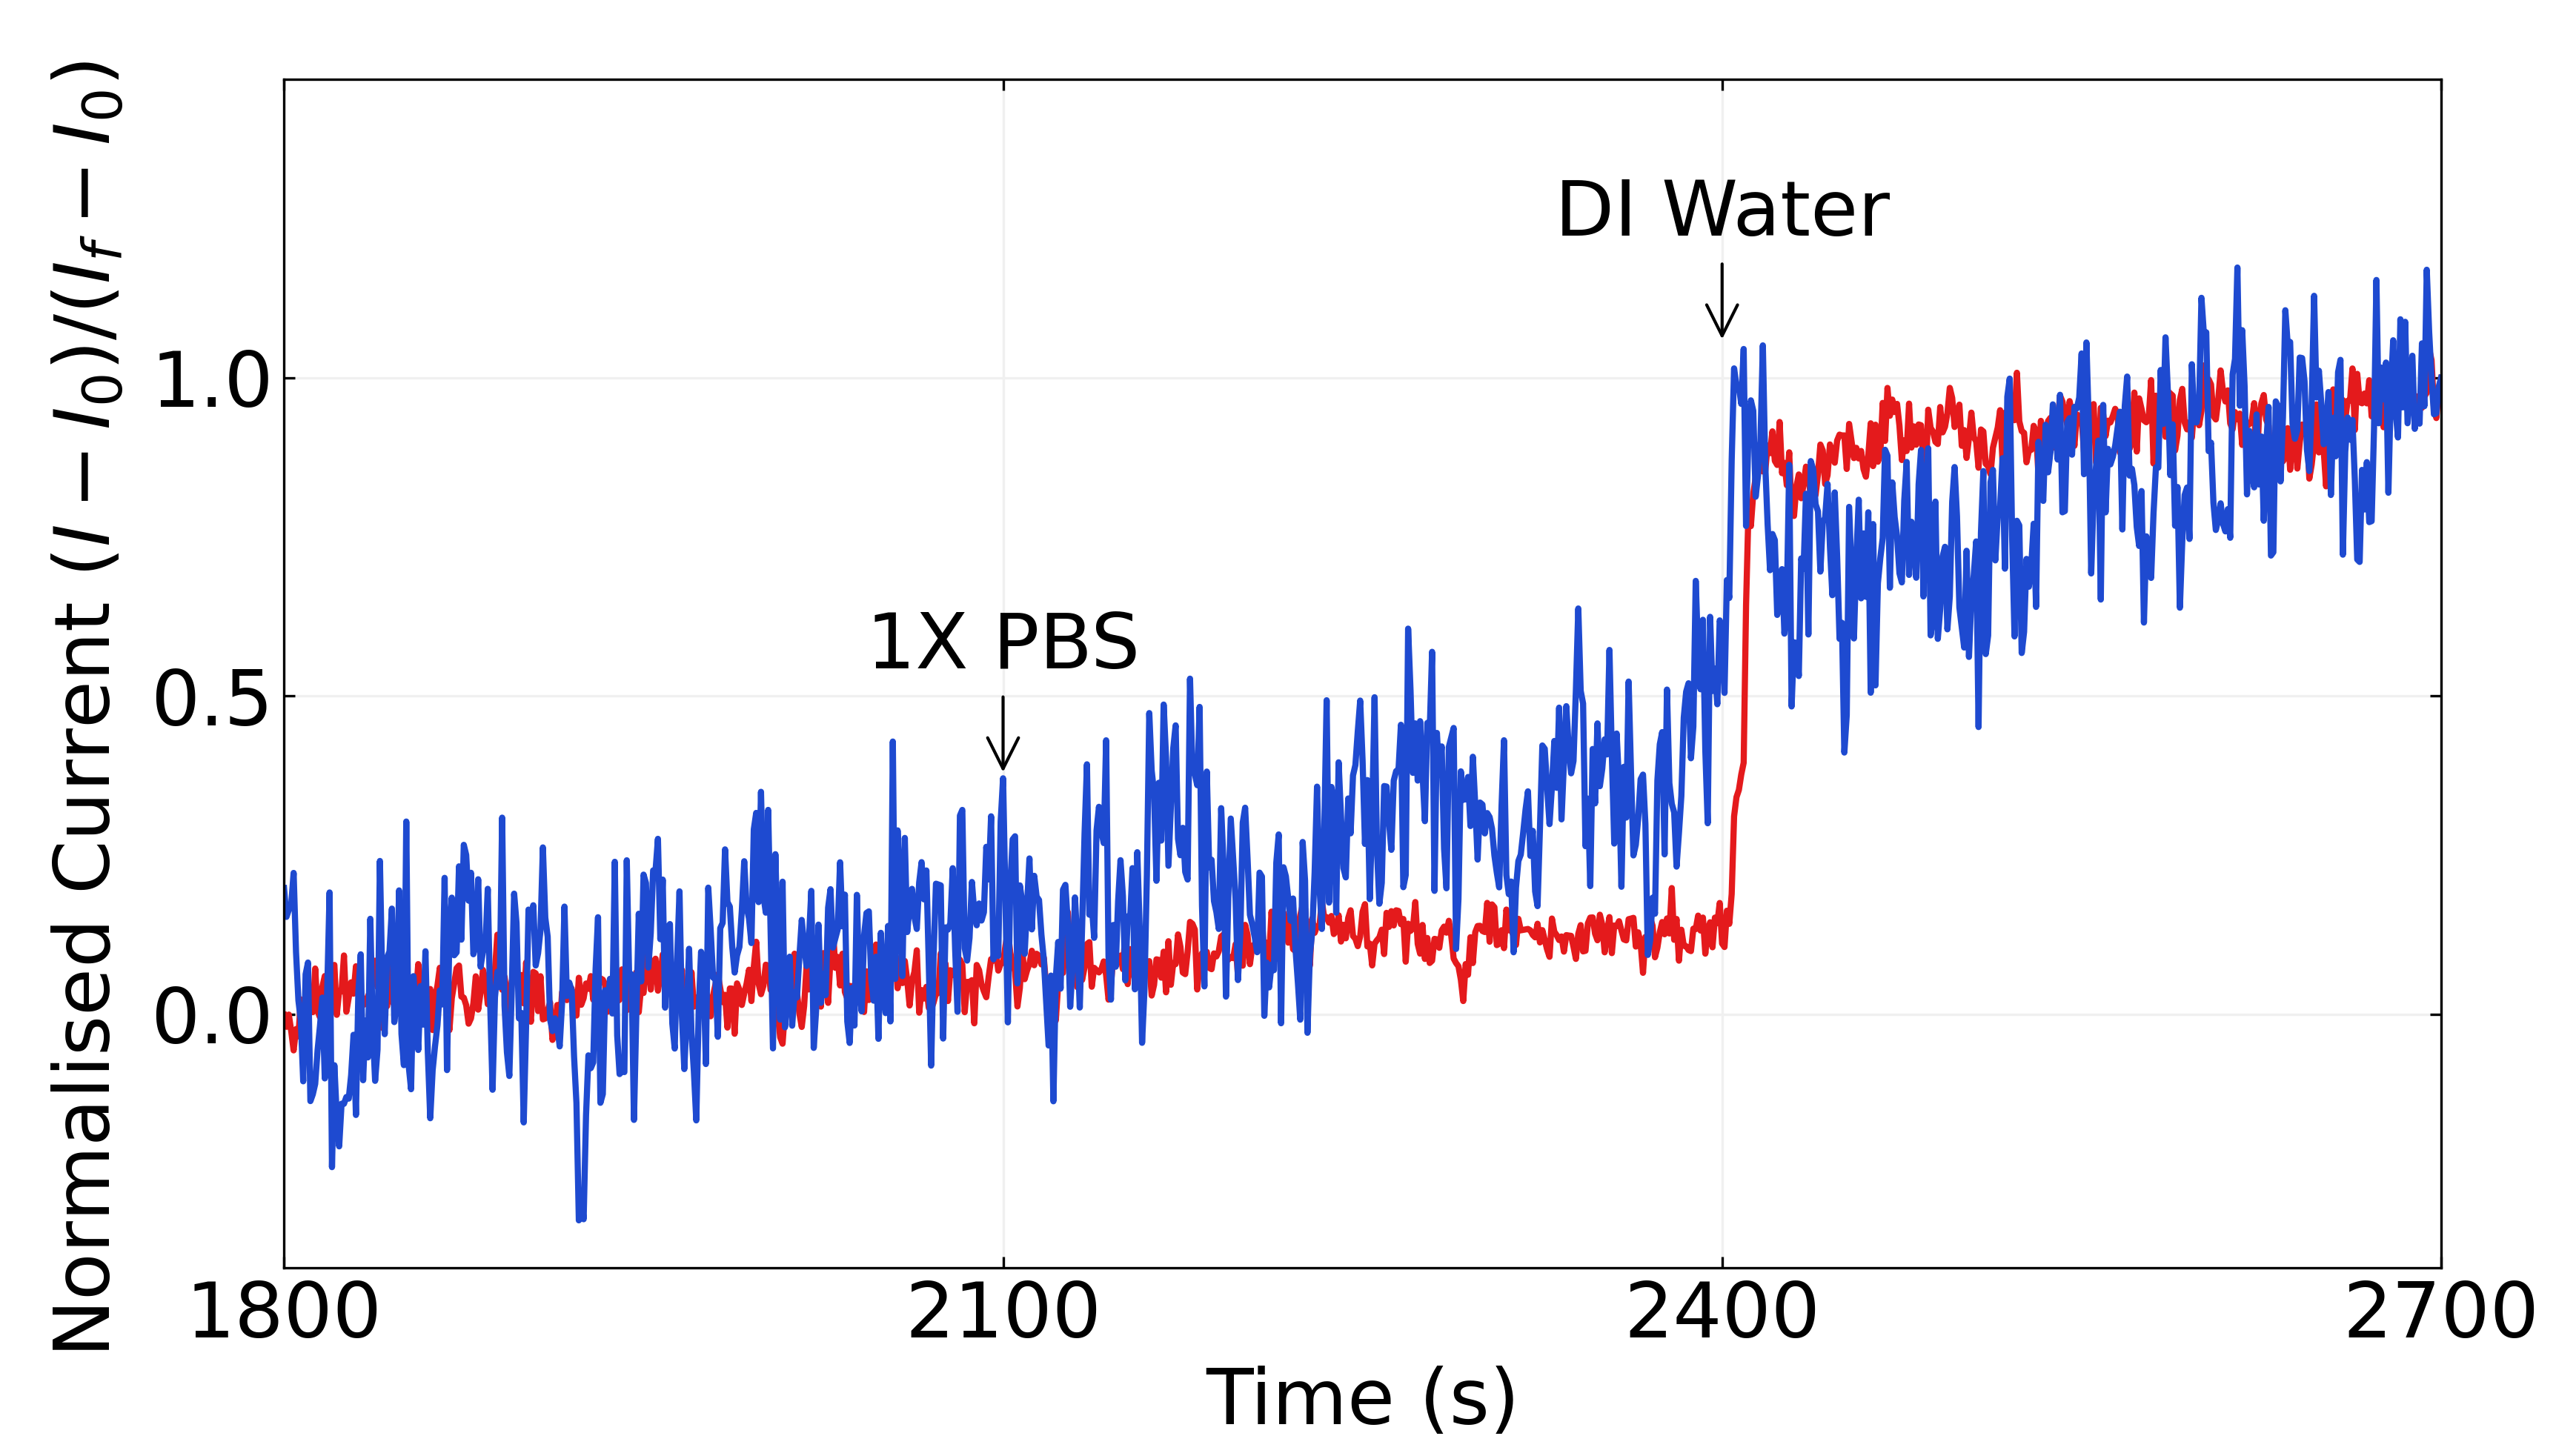
\includegraphics{figures/ch6/saltconc_initial_additions.png}

}

}

\subcaption{\label{fig-salt-conc-SNR}}
\end{minipage}%

\caption{\label{fig-salt-conc-SNR}The transfer characteristics of a
single steam-deposited carbon nanotube field-effect transistor channel
are shown in (a). V\(_{gap}\) is the gate voltage corresponding to the
center of the transistor bandgap, found at the minimum of the
characteristic curve. The signal-to-noise ratio of the channel response
to a deionised water addition after a suitable control series is shown
in (b). The blue current trace in (b) was performed gating the device
150 mV away from V\(_{gap}\), while the red current was performed gating
the device 200 mV away from V\(_{gap}\).}

\end{figure}

To understand the effect of gate voltages on signal-to-noise ratio, two
PBS control and salt concentration sensing series were performed with
the same channel at different gate voltages. The transfer
characteristics of this channel are shown in
Figure~\ref{fig-transfer-sweep-2}, with coloured dashed lines marking
the voltages used for gating the transistor during each sesning series.
Figure~\ref{fig-salt-conc-SNR} shows the initial PBS and DI water
additions made after 1800 s. Previous work on the signal-to-noise ratio
for liquid-gated, encapsulated carbon nanotube devices suggests that
gating devices close to \(V_{gap}\) should give the largest
signal-to-noise ratio for salt concentration additions
\autocite{Heller2009}. However, this was not what was observed for our
carbon nanotube field-effect transitor, as
Figure~\ref{fig-salt-conc-SNR} shows improved signal-to-noise ratio,
i.e.~the signal step can be more clearly distinguished, when gated at a
voltage further removed from \(V_{gap}\). This discrepancy could be a
result of the use of a network of carbon nanotubes rather than a single
nanotube; gating may have less of an impact on noise when a network
morphology is used. Alternatively, it could be a result of a lack of
mixing in our static well setup leading to inconsistent signal sizes
with concentration change. Heller \emph{et al.} used a flow cell during
their signal-to-ratio work \autocite{Heller2009}. By using a flow cell
with our devices, it would be possible to confirm whether this is the
case, and this might also help us reduce the size of unwanted transient
responses resulting from drop-wise additions.

\hypertarget{sec-pristine-EtHex}{%
\section{Vapour Sensing with Ethyl Hexanoate}\label{sec-pristine-EtHex}}

\hypertarget{sec-vapour-drift}{%
\subsection{Baseline Drift}\label{sec-vapour-drift}}

When sensing vapour in the vapour delivery system, devices have no
liquid gate and are instead backgated when taking measurements.
Therefore, the baseline drift of devices characterised in this manner
should be considered separately to those characterised in an
liquid-gated environment. Device baseline drift of a backgated device in
the vapour sensing chamber is therefore examined here in more detail. A
AZ\(^\circledR\) 1518 encapsulated carbon nanotube network device was
used in this discussion. The device was fabricated on a substrate with a
300 nm SiO\(_2\) layer, and the carbon nanotube film was deposited using
the steam-assisted surfactant method. Before measurements were taken,
the vapour system was purged of vapour, the total dilution flow into the
chamber was set at 200 sccm as read by the Tylan mass flow controller
and flow to the PID was set to 150 sccm on the flowmeter. The transfer
sweep of a channel on this device (channel 6) is shown in
Figure~\ref{fig-backgate-transfer}, measured using the B1500A
semiconductor device analyser.

\begin{figure}

{\centering \includegraphics[width=0.35\textwidth,height=\textheight]{figures/ch6/Q2C6_backgate_characterisation.png}

}

\caption{\label{fig-backgate-transfer}Transfer sweep of a
steam-deposited carbon nanotube network field-effect transistor,
backgated in the vapour delivery system device chamber.}

\end{figure}

\begin{figure}

\begin{minipage}[t]{0.15\linewidth}

{\centering 

~

}

\end{minipage}%
%
\begin{minipage}[t]{0.70\linewidth}

{\centering 

\includegraphics{figures/ch6/Q2C6_fitted_curves_edited.png} {}

}

\end{minipage}%
%
\begin{minipage}[t]{0.15\linewidth}

{\centering 

~

}

\end{minipage}%
\newline
\begin{minipage}[t]{0.15\linewidth}

{\centering 

~

}

\end{minipage}%
%
\begin{minipage}[t]{0.70\linewidth}

{\centering 

\includegraphics{figures/ch6/Q2C6_fitted_curves_exp_edited.png} {}

}

\end{minipage}%
%
\begin{minipage}[t]{0.15\linewidth}

{\centering 

~

}

\end{minipage}%

\caption{\label{fig-bg-baseline-drift}The source-drain and gate current
measured for a backgated device channel across 3600 s, where V\(_ds\) =
100 mV and V\(_g\) = 0 V is shown in (a). A linear fit to the data from
2400 s onwards has been indicated on (a) with a black dashed line. The
linear fit has then been subtracted from (a) to give the dataset shown
in (b). An exponential fit to the dataset in (b) is also shown in black.
The R-squared value for the linear fit in (a) was 0.998, while the
R-squared value for the exponential fit in (b) was 0.89.}

\end{figure}

Figure~\ref{fig-bg-baseline-drift} (a) shows 3600 s of baseline drift
from the same channel when the device was backgated at V\(_g\) = 0 V and
a source-drain voltage of V\(_{ds}\) = 100 mV was placed across the
channel. During this period of time, a 200 sccm nitrogen flow was placed
through the device chamber with the dilution mass flow controller. Gate
leakage current remains negligible across the entire control series. As
seen for the liquid-gated device in Section~\ref{sec-baseline-drift},
there is a period of rapid exponential decay followed by a period of
stable, approximately linear baseline drift. The baseline drift observed
here appears to be significantly lower than that seen by Noyce \emph{et
al.} \autocite{Noyce2019}. This observation suggests that the higher
magnitude of drift observed by Noyce \emph{et al.} is not a result of
backgating in air, as previously suggested, but instead due to the use
of a significantly different fabrication process for their devices.

A linear least-squares fit was performed on the samples taken between
2400 s \(-\) 3600 s, and the fit obtained had an R-squared value of
0.998. The constants obtained for the linear fit, where
\(I = c_1t + c_2\), were \(c_1 = -17.31\pm0.05\) pAs\(^{-1}\) and
\(c_2 = 0.779 \mu\)A. Both linear and constant terms are slightly higher
than that of the average liquid-gated device drift. The linear fit was
then subtracted from the raw data, and an exponential least-squares fit
was performed on the remaining dataset.
Figure~\ref{fig-bg-baseline-drift} (b) shows the exponential fit to this
remaining dataset from 0 s \(-\) 3600 s, where the R-squared value was
0.89. The constants obtained for the exponential fit
\(I = I_0exp(-t/\tau)\) were \(I_0 = 7.20 \pm 0.05\) nA and
\(\tau = 730 \pm 10\). The exponential term is very similar in size and
time constant to those of the liquid-gated device, which may indicate
this decay behaviour is independent of the type of transistor gating.
The large time constant indicates that 3600 s is just sufficient for the
exponential term to decay to approximately zero before starting a
sensing series for this channel.

This analysis indicates that the baseline drift for the backgated carbon
nanotube under nitrogen flow can be approximated as a combination of a
exponential, linear and constant term. Furthermore, while only measured
here for a single channel, it appears likely that we can expect
backgated baseline drift behaviour to be similar to the multiplexed
liquid-gated drifts observed in Section~\ref{sec-baseline-drift}. It
seems that the nature of baseline drift in these devices is largely a
result of the general nature of the carbon nanotube network, rather than
the type of gating used for device characterisation.

\hypertarget{sec-EtHex-series}{%
\subsection{Sensing Series}\label{sec-EtHex-series}}

Directly after the 3600 s control series, the device was exposed to four
intervals of ethyl hexanoate vapour flow from the carrier line. 5 mL of
ethyl hexanoate was placed into the analyte bottle on the carrier line
before testing for the sensing series. The same settings for the vapour
delivery system were kept from Section~\ref{sec-vapour-drift}. A total
flow of 200 sccm between the two mass flow controllers was kept through
the chamber at all times. During each interval 150 sccm flow was placed
through the carrier line. Apart for the duration of these intervals,
flow through the carrier line was kept at zero. The intervals were of
varying lengths to see how the carbon nanotube device responded to
various concentrations of vapour in the chamber as recorded by the PID.
A 1200 s recovery period was placed between each carrier flow interval,
where 200 sccm flow was placed into the chamber from the dilution line.
A separate test was also performed in an identical manner, except no
ethyl hexanoate was placed into the analyte bottle. The chamber
temperature was 22°C \(\pm\) 2°C for all measurements.

\begin{figure}

\begin{minipage}[t]{0.15\linewidth}

{\centering 

~

}

\end{minipage}%
%
\begin{minipage}[t]{0.70\linewidth}

{\centering 

\includegraphics{figures/ch6/Q2C6_Q3C2_detrend_trunc_arrows_normalised_edited.png}
{}

}

\end{minipage}%
%
\begin{minipage}[t]{0.15\linewidth}

{\centering 

~

}

\end{minipage}%
\newline
\begin{minipage}[t]{0.15\linewidth}

{\centering 

~

}

\end{minipage}%
%
\begin{minipage}[t]{0.70\linewidth}

{\centering 

\includegraphics{figures/ch6/Q2C6_Q3C2_mean_simple_difference_before_and_after_edited.png}
{}

}

\end{minipage}%
%
\begin{minipage}[t]{0.15\linewidth}

{\centering 

~

}

\end{minipage}%

\caption{\label{fig-EtHex-sampling}Device channel responses to intervals
of flow from the carrier line into the vapour delivery system chamber.
Intervals begin at 3600 s, 4850 s, 6150 s and 7500 s. The length of each
interval is indicated above the corresponding normalised current
responses in (a) for both ethyl hexanoate (EtHex) and for no analyte
present in the analyte bottle. The signal changes corresponding to the
current responses to each interval for both ethyl hexanoate and for no
analyte present are shown in (b).}

\end{figure}

Figure~\ref{fig-EtHex-sampling} shows the result of these interval
tests, both with and without ethyl hexanoate placed in the analyte
bottle. The data presented in Figure~\ref{fig-EtHex-sampling} (a) has
been normalised, despiked, filtered and corrected for baseline drift in
the manner described in both Section~\ref{sec-python-analysis} and
Section~\ref{sec-salt-conc-series}. Each interval of exposure to carrier
line flow corresponds to a current increase. These increases have been
labelled with the length of the corresponding interval used. When ethyl
hexanoate is present in the analyte bottle on the carrier line, the
response to each exposure interval is considerably larger than the
response when no analyte is present. It should be noted that some
response to carrier line flow is observed even when the analyte bottle
is empty. This is most likely to be the result residual analyte in the
carrier line being pumped into the chamber. It appears very low levels
of analyte persist in the line even after purging the system lines with
a roughing pump. Concentration measurements taken using the
photoionisation detector, shown in Figure~\ref{fig-EtHex-sampling-PID},
also indicate some low-level, residual vapour reaches the chamber during
each interval even when the analyte bottle is left empty.

\begin{figure}

{\centering \includegraphics[width=0.7\textwidth,height=\textheight]{figures/ch6/input_time_comparison.png}

}

\caption{\label{fig-EtHex-sampling-PID}Nominal concentration
measurements by the photoionisation detector taken from the device
chamber during device current sampling from 3600 s onwards, both with
and without ethyl hexanoate (EtHex) in the analyte bottle. The maximum
nominal concentration reached during each carrier flow interval is
indicated above each peak.}

\end{figure}

The signal response seen corresponds to a change in conductance of the
exposed carbon nanotubes within the device channel. These conductance
changes occur due to the molecular adsorption of ethyl hexanoate vapour
onto the external and internal surfaces of the nanotubes. The vapour can
dopes the semiconducting carbon nanotubes in the channel, causing a
shift in the channel threshold voltage, and can cause carrier scattering
when adsorped onto the metallic nanotubes present. Binding of analyte to
a gas sensing material can be reversible or irreversible. In general,
adsorption onto carbon nanotube sensors is irreversible. This
irreversibility means after a response to analyte, readings from the
sensor will not return to the original baseline within the same
timescale as the sensing response, even after stopping analyte flow to
the chamber \autocite{Agnihotri2005,Lee2005}. From
Figure~\ref{fig-EtHex-sampling}, it is clear that the carbon nanotube
sensor configuration used here is primarily irreversible, where the
current level does not return to baseline within a period of 1200 s
after analyte exposure.

\begin{figure}

{\centering \includegraphics[width=0.55\textwidth,height=\textheight]{figures/ch6/EtHex-ratio-comparison.png}

}

\caption{\label{fig-EtHex-ratio-comparison}Device response against
maximum concentration measurement corresponding to each interval of
carrier flow. The experimental results have been fitted with two
adsorption isotherm models. The chamber temperature was 22°C ± 2°C
across both datasets.}

\end{figure}

Assuming that the signal response is directly proportional to the degree
of surface coverage by adsorbed analyte on the carbon nanotube network
\autocite{Lee2005}, it should be possible to model the relationship
between signal response and concentration in the device chamber with an
adsorption isotherm \autocite{Agnihotri2005}.
Figure~\ref{fig-EtHex-ratio-comparison} shows the maximum nominal
concentration measured for every peak shown in
Figure~\ref{fig-EtHex-sampling-PID} plotted against the corresponding
signal responses shown in Figure~\ref{fig-EtHex-sampling} (b). The
Freundlich adsorption isotherm (Equation~\ref{eq-freundlich}) models
adsorption onto a heterogeneous surface. \(K_F\) is the adsorption
capacity and \(1/n\) is adsorption intensity. \(1/n\) can be used to
understand the heterogeneity of adsorbate sites
\autocite{Ayawei2017,Sabzehmeidani2021}. The vapour response factor is
denoted as \(k_{RF}\), which is equal to 1.6 for a 10.6 eV
photoionisation detector (PID). As the PID has been run uncalibrated, a
factor \(k_{D}\) has been included to account for linear span drift. As
span drift due to window contamination can cause concentration readings
to be reduced up to 30\% after six months of PID operation, it is
expected that \(k_{D}\) falls within the range of 0.2 \(-\) 1
\autocite{PIDmanual,Ionscience}.
\begin{equation}\protect\hypertarget{eq-freundlich}{}{
q_e = K_F(k_Dk_{RF}C_e)^{1/n}
}\label{eq-freundlich}\end{equation}

The isotherm has previously been used to model adsorption of volatile
organic molecules onto single-walled carbon nanotubes
\autocite{Agnihotri2005}. The best-fit Freundlich isotherm is also shown
in Figure~\ref{fig-EtHex-ratio-comparison}, fitted using linear
least-squares methods with an R-squared value of 0.921. This isotherm
had an \(n\) value of \(n = 2.1\pm1.1\).

\hypertarget{conclusion}{%
\section{Conclusion}\label{conclusion}}

To ensure fabricated transistors were suitable for biosensing purposes,
the morphology and electrical properties of the pristine carbon nanotube
and graphene transistors were investigated.

The morphology of the carbon nanotube networks were found to have a
significant impact on the electrical characteristics of the devices,
which was determined through comparison of the skew-normal height
profile of the carbon nanotube network and the key electrical parameters
of a range of carbon nanotube devices. When networks were highly bundled
(\(>90\)\%), there was a large range of carbon nanotube bundle diameters
present in the network. This large variation in the size of conducting
pathways resulted in a wide range of on-off ratios and threshold
voltages for the liquid-gated devices created using these carbon
nanotube films. In contrast, devices using films fabricated with a
relatively low percentage of bundling (\(<75\) \%) showed highly
consistent on-off ratios and threshold voltages, along with low
hysteresis, due to the relatively consistent bundle diameters and high
density of these networks. These low-bundling networks were found to
have a mean bundle distribution height of \(3.3 \pm 1.0\) nm. When
performing multiplexed sensing, consistent channel behaviour is highly
desirable since comparing sensing behaviour between channels is more
straightforward.

However, atomic force microscope imaging and Raman spectroscopy also
indicated that less bundled networks had the most surface contamination
present. Aggregated surfactant present on the surface had a height of
more than 4 nm, and introduced significant defects to the carbon
nanotube network. The introduction of \(p\)-dopants to the carbon
nanotubes by surfactant appears to have significantly increased the
threshold voltage of steam-assisted surfactant-deposited network devices
relative to steam-free surfactant-deposited network devices. Since the
presence of surfactant could negatively impact biosensing, techniques to
remove contaminants should be explored in more detail. Oxidation and
thermal annealing of carbon nanotube films at high temperatures could be
used to resolve this issue, and this is discussed further in
\textbf{?@sec-future-work}. The presence of electrolyte on the surface
of a backgated transistor for use in vapour sensing was also found to
significantly adversely affect its electrical characteristics.

Constant voltage real-time measurements of the carbon nanotube
field-effect transistor devices had a characteristic drift that could be
modelled using a exponential and linear term. The linear term of
baseline drift had a reasonably consistent gradient between device
channels, with a mean value of \(-6.1 \pm 1.2\), indicating that similar
drift behaviour should be reproducible between devices fabricated in the
same manner. The time constant of the exponential term ranged from
\(\tau = 330 \pm 20\) s to \(\tau = 800 \pm 750\) for the device
characterised. These results indicate that the PBS control series is
asuitable time length for minimising the effects of baseline drift on
sensing, since the range of time constants are all well below the total
timescale of the control series.

Salt concentration or PBS dilution sensing series indicated that the
carbon nanotube transistor devices were highly sensitive to
environmental changes and therefore suitable for sensing work.
Successive additions of deionised water to the 1XPBS present in the well
gave signal responses of up to 2.5 \% above the control response. The
signal response was found to be proportional to the logarithm of
concentration, giving a fit to the median response sizes with an
\(R^2 = 0.86\). Deviations from this trend can possibly be explained by
the enclosed sensing environment preventing sufficient mixing of
electrolyte concentrations within the PDMS well, which could possibly be
addressed by using a flow cell for sensing work. It was also seen that
the signal size relative to baseline drift was highly consistent between
channels. This is a promising result when it comes to ensuring
consistent multiplexing, but it cannot be guaranteed that this behaviour
carries over to sensing with biofunctionalised devices.

Graphene field-effect transistor devices were often found to possess a
double-minima feature, which appears to be the result of a lack of
doping from the metal contacts in the center of the device channels.
These double Dirac points are unlikely to have an significant effect on
the sensing behaviour of graphene devices. The graphene device
characteristics were found to be consistent after 1 hour exposure to 1X
PBS with minimal drift, with an on-off ratio of 5 and major Dirac point
voltage of 0.3 V. There was some indications from the transfer
characteristics that \(p\)-dopants were present on the graphene surface.
Salt concentration sensing with graphene FETs is not shown in this
thesis, but it is important to perform this experiment and use similar
analysis techniques if there are any concerns about the sensitivity of a
fabricated batch of graphene devices.

\cleardoublepage
\phantomsection
\addcontentsline{toc}{part}{Appendices}
\appendix

\hypertarget{sec-vapour-sensor-components}{%
\chapter{Vapour System Hardware}\label{sec-vapour-sensor-components}}

\hypertarget{tbl-vapour-sensor-components}{}
\begin{longtable}[t]{>{\raggedright\arraybackslash}p{5.5cm}>{\raggedright\arraybackslash}p{4.5cm}>{\raggedright\arraybackslash}p{3.75cm}}
\caption{\label{tbl-vapour-sensor-components}Major components used in construction of the vapour delivery system
described in this thesis. }\tabularnewline

\toprule
Description & Part No. & Manufacturer\\
\midrule
Mass flow controller, 20 sccm full scale & GE50A013201SBV020 & MKS Instruments\\
Mass flow controller, 200 sccm full scale & GE50A013202SBV020 & MKS Instruments\\
Mass flow controller, 500 sccm full scale & FC-2901V & Tylan\\
Analogue flowmeter, 240 sccm max. flow & 116261-30 & Dwyer\\
Micro diaphragm pump & P200-B3C5V-35000 & Xavitech\\
\addlinespace
Analogue flow controller, for micro diaphragm pump & X3000450 & Xavitech\\
10 mL Schott bottle & 218010802 & Duran\\
PTFE connection cap system & Z742273 & Duran\\
Baseline VOC-TRAQ flow cell, red & 043-951 & Mocon\\
Humidity and temperature sensor & T9602 & Telaire\\
\addlinespace
Enclosure, for humidity and temperature sensor & MC001189 & Multicomp Pro\\
\bottomrule
\end{longtable}

\hypertarget{sec-python}{%
\chapter{Python Code for Data Analysis}\label{sec-python}}

\hypertarget{code-repository}{%
\section{Code Repository}\label{code-repository}}

The code used for general analysis of field-effect transistor devices in
this thesis was written with Python 3.8.8. Contributors to the code used
include Erica Cassie, Erica Happe, Marissa Dierkes and Leo Browning. The
code is located on GitHub and the research group OneDrive, and is
available on request.

\hypertarget{sec-histogram-analysis}{%
\section{Atomic Force Microscope Histogram
Analysis}\label{sec-histogram-analysis}}

The purpose of this code is to analyse atomic force microscope (AFM)
images of carbon nanotube networks in .xyz format taken using an atomic
force microscope and processed in Gwyddion (see
\textbf{?@sec-afm-characterisation}). It was originally designed by
Erica Happe in Matlab, and adapted by Marissa Dierkes and myself for use
in Python. The code imports the .xyz data and sorts it into bins 0.15 nm
in size for processing. To perform skew-normal distribution fits, both
\emph{scipy.optimize.curve\_fit} and \emph{scipy.stats.skewnorm} modules
are used in this code.

\hypertarget{sec-raman-analysis}{%
\section{Raman Spectroscopy Analysis}\label{sec-raman-analysis}}

The purpose of this code is to analyse a series of Raman spectra taken
at different points on a single film (see
\textbf{?@sec-raman-characterisation}). Data is imported in a series of
tab-delimited text files, with the low wavenumber spectrum (100
cm\(^{-1} - 650\) cm\(^{-1}\)) and high wavenumber spectrum (1300
cm\(^{-1} - 1650\) cm\(^{-1}\)) imported in separate datafiles for each
scan location.

\hypertarget{sec-field-effect-transistor-analysis}{%
\section{Field-Effect Transistor
Analysis}\label{sec-field-effect-transistor-analysis}}

The purpose of this code is to analyse electrical measurements taken of
field-effect transistor (FET) devices. Electrical measurements were
either taken from the Keysight 4156C Semiconductor Parameter Analyser,
National Instruments NI-PXIe or Keysight B1500A Semiconductor Device
Analyser as discussed in \textbf{?@sec-electrical-characterisation}; the
code is able to analyse data in .csv format taken from all three
measurement setups. The main Python file in the code base consists of
three related but independent modules: the first analyses and plots
sensing data from the FET devices, the second analyses and plots
transfer characteristics from channels across a device, and the third
compares individual channel characteristics before and after a
modification or after each of several modifications. The code base also
features a separate config file and style sheet which govern the
behaviour of the main code. The code base was designed collaboratively
by myself and Erica Cassie over GitHub using the Sourcetree Git GUI.


\backmatter
\printbibliography


\end{document}
